%Ultimatives Tool zur Datierung:
%https://www.cc.kyoto-su.ac.jp/~yanom/pancanga/
%skp = ignored in edition
%skm = ignored in xml
%%%---2-DO---%%%:
% - add xml ids for cladistics
% - produce diplomatic transcripts for saktumiva
% - read Sarvangayogapradipika, Maya Burger! 
% - maybe add second ciritical edition of yogasvarodaya?!
% - grep-search alle Verse!!!!
% - Mss spreadsheet
% - additions to U2: make footnotes for the bahir mātrā-s: explaining the inventions of female deities and tell that this is "schwer interpretierbar"
% - Consider changing Lakṣya to Lakṣa
%%%%%%%%%%%%%%%%%%%%%%%%%%%%%%%%%%%%%%%%%
% Don't forget
% Siddhasiddhantapaddhati Yogic Body descriptions are followed by Rāmacandra
% Quotes of the Yogasvarodaya in the Yoga Karṇikā
% Rāmacandra more a compiler than an author!!!
% Identify quotes of YTB in Haṭhasanketacandrikā -- done :D
%%%%%%%%%%%%%%%%%%%%%%%%%%%%%%%%%%%%%%%%%%%
%MSS notes
%
%--B: i and ī are not differenciated
%--P: no punctuation no daṇdas nothing
%--U1: dot . serves as daṇḍa 
%--\L and \U2 very similar
%--figure out for U2: // ajapājapaḥ sahasra // 6000 //gha 0 16 pa 0 40// \U2?!?!?!?!?!?
%%%%%%%%%%%%%%%%%%%%%%%%%%%%%%%%%%%%%%%%%%
%
% Einleitung Ideen 
% - sprachliche Simplizität
% - Potenzial als Anfängertext
% - Großartige Einführung in die Textkritik -> Synoptische Edition 
% - Gelegenheit Yogasvarodaya und Yogatattvabindu zu edieren 
% - Historische Evidenz entweder für das königliche Leben in einer Maṭha in der Nähe von Benares während der Muslimischen Herrschaft, oder sogar Lehrtext für die Bildung junger Prinzen  
% - eines der raren Beispiele der engen Verknüfung mehrerer Texte 
% - eines der raren Beispiele der Prosaisierung eines metrischen Textes 
% - Anwendung rezenter Technologie! 
% - How the text was construed -> intermingling of Ysv and SSP
% - Martin Straube: "jeder kleine Dorfhäuptling kann Rāja genannt werden". 
%%%%%%%%%%%%%%%%%%%%%%%%%%%%%%%%%%%%%%%%%%%
\documentclass[10pt]{memoir}
\setstocksize{220mm}{155mm} 	        
\settrimmedsize{220mm}{155mm}{*}	
\settypeblocksize{170mm}{116mm}{*}	
\setlrmargins{18mm}{*}{*}
\setulmargins{*}{*}{1.2}
%\setlength{\headheight}{5pt}%
\checkandfixthelayout[lines]
\linespread{1.16}
\flushbottom

%%% Hyphenation settings
\usepackage[htt]{hyphenat}
\hyphenation{he-lio-trope opos-sum}
\tracingparagraphs=1
%Hyphenation in Devanāgarī of the edition still missing? Probably this needs to be modified in babel-iast package? 

%%% babel
\usepackage[english]{babel}
\usepackage{babel-iast/babel-iast}

\babelfont[iast]{rm}[Renderer=Harfbuzz, Scale=1.3]{AdishilaSan}%AdishilaSan}
\babelfont[english]{rm}{Adobe Text Pro}

%%% more functionality
\PassOptionsToPackage{hyphens}{url}
\usepackage{hyperref}
\usepackage{pdflscape}
\usepackage{cleveref}
\usepackage{url}
\usepackage{cleveref}
\usepackage{microtype}
\usepackage{lineno}

%\usepackage{bigfoot}
%%% more functions
\usepackage[dvipsnames]{xcolor}
%\usepackage[para,perpage]{footmisc}

%%%für den Counter von Kapiteln und Sätzen! 
\newcommand{\uproman}[1]{\uppercase\expandafter{\romannumeral#1}}
\newcommand{\lowroman}[1]{\romannumeral#1\relax}

\makeindex
\newfontfamily\sanskritfont[Script=Devanagari,Mapping=RomDev,Scale=1.1]{Sanskrit2003}
\usepackage{pifont,fourier-orns,lettrine,psvectorian,paralist,enumitem,pdfpages,wrapfig,tabulary,lettrine,longtable}
\setlist[enumerate]{itemsep=0mm}
\usepackage[autostyle]{csquotes}
\usepackage[defaultlines=2,all]{nowidow}
\usepackage{ellipsis,adforn,booktabs,longtable,url,tikz}
\lineskiplimit=-3pt          

\makechapterstyle{IeT}{%
  \chapterstyle{default}
  \renewcommand*{\printchapternonum}{\centering}
  \renewcommand*{\clearforchapter}{\cleartorecto} 
  \aliaspagestyle{chapter}{empty}}
\chapterstyle{IeT}
\setsecnumdepth{none}  \openright  \nouppercaseheads
\settocdepth{subsubsection}

%%%% test better pagebreaks
%\def\fussy{%
%  \emergencystretch\z@
%  \tolerance 200%
%  \hfuzz .1\p@
%  \vfuzz\hfuzz}

%\interfootnotelinepenalty=10000\relax

%\usepackage[maxfloats=256]{morefloats}

%\maxdeadcycles=500

%raggedbottomsectiontrue
%%\checkandfixthelayout


%%%%%%%  biblatex
%\newcommand{\noun}[1]{\textsc{#1}}    %  philosophy-verbose
\usepackage[backend=biber, sorting=nyt, style=verbose]{biblatex} %%%%ORIGINAL TiE
\renewcommand*{\mkbibnamefamily}[1]{\textsc{#1}}


\DeclareFieldFormat{url}{%
  \mkbibacro{URL}\addcolon\space
  \href{#1}{\nolinkurl{\thefield{urlraw}}}}

\DeclareFieldFormat{citeurl}{%
  \href{#1}{\nolinkurl{\thefield{urlraw}}}} 


\DeclareFieldFormat{postnote}{#1}
\renewcommand{\postnotedelim}{, }
\addbibresource{bindu.bib}

%%% ekdosis
\usepackage[teiexport=tidy,parnotes=true]{ekdosis}% =tidy cleans up HTML and XML documents by fixing markup errors and upgrading legacy code to modern standards. parnotes=footnotes below or above critical apparatus

\SetLineation{lineation=page, modulo} %lineation=page sets thenumbering to start afresh at the top of each page. =modulo makes every fifth line numbered. {lineation=page} makes every line numbered! 

\renewcommand{\linenumberfont}{\selectlanguage{english}\footnotesize} %sets language of lines to English

\SetTEIxmlExport{autopar=false} %autopar=falseinstructs ekdosis to ignore blank lines in the.tex sourcefile as markers for paragraph boundaries. As a result, each paragraph of the edition must be found within an environment associated with the xml <p> element

\SetHooks{
  lemmastyle=\bfseries,
  %refnumstyle=\selectlanguage{english}\bfseries,
  refnumstyle=\selectlanguage{english}\color{blue}\bfseries,
  appheight=0.8\textheight,
}

\newif\ifinapparatus
\DeclareApparatus{source}[
%bhook=\inapparatustrue,
lang=english,
notelang=english,
% bhook=\selectlanguage{english},
bhook=\selectlanguage{english}\textbf{Sources:},%
%maxentries=4, 
%ehook=.]
%sep={] },
%nosep,
]

\newif\ifinapparatus
\DeclareApparatus{testium}[
%bhook=\inapparatustrue,
lang=english,
notelang=english,
% bhook=\selectlanguage{english},
bhook=\selectlanguage{english}\textbf{Testimonia:},
%maxentries=4, 
%ehook=.]
%nosep, 
]

% Declare \ifinapparatus and set \inapparatustrue at the beginning of
% the apparatus criticus block. Also set the language.  
\newif\ifinapparatus
  \DeclareApparatus{default}[
  %bhook=\inapparatustrue, 
  lang=english,
  %maxentries=33,
  %bhook=\selectlanguage{english},
  sep = {] },
  delim=\hskip 0.75em,
  rule=\rule{0.7in}{0.4pt},
]

\newif\ifinapparatus
\DeclareApparatus{philcomm}[
%bhook=\inapparatustrue,
lang=english,
notelang=english,
bhook=\selectlanguage{english}\textbf{Philological Commentary:},
%bhook=\selectlanguage{english},
sep={: },
]

\ekdsetup{
showpagebreaks,
spbmk = \textcolor{blue}{spb},
hpbmk = \textcolor{red}{hpb}
}

%\usepackage{fnpos}
%\makeFNmid
%\makeFNbottom
\usepackage[bottom]{footmisc}
%%%%%%%%%%%%%%%%%%%%%%%%%%%
\makeatletter
\def\blfootnote{\gdef\@thefnmark{}\@footnotetext}
\makeatother
%%%%%%%%%%%%%%%%%%%%%%%%%


% Macros and Definitions for the Print of Sigla
\def\acpc#1#2#3{{#1}\rlap{\textrm{\textsuperscript{#3}}}\textsubscript{\textrm{#2}}\space}
\def\sigl#1#2{{{#1}}\textsubscript{\textrm{#2}}}
\def\None{{\sigl{N}{1}}} \def\Noneac{\acpc{N}{1}{ac}\,} \def\Nonepc{\acpc{N}{1}{pc}\,}
\def\Ntwo{{\sigl{N}{2}}} \def\Noneac{\acpc{N}{2}{ac}\,} \def\Nonepc{\acpc{N}{2}{pc}\,}
\def\Done{{\sigl{D}{1}}} \def\Doneac{\acpc{D}{1}{ac}\,} \def\Donepc{\acpc{D}{1}{pc}\,}
\def\Dtwo{{\sigl{D}{2}}} \def\Dtwoac{\acpc{D}{2}{ac}\,} \def\Dtwopc{\acpc{D}{2}{pc}\,}
\def\Uone{{\sigl{U}{1}}} \def\Uoneac{\acpc{U}{1}{ac}\,} \def\Uonepc{\acpc{U}{1}{pc}\,}                 
\def\Utwo{{\sigl{U}{2}}} \def\Utwoac{\acpc{U}{2}{ac}\,} \def\Utwopc{\acpc{U}{2}{pc}\,}

%%%%%%%%%%%%%% Tattvabinduyoga - List of Witnesses   %%%%%%%%%%%%%%%%%%%
\DeclareWitness{ceteri}{\selectlanguage{english}cett.}{ceteri}[]   
\DeclareWitness{E}{\selectlanguage{english}E}{Printed Edition}[]    
\DeclareWitness{P}{\selectlanguage{english}P}{Pune BORI 664}[]  
\DeclareWitness{B}{\selectlanguage{english}B}{Bodleian 485}[]       
\DeclareWitness{N1}{\selectlanguage{english}N\textsubscript{1}}{NGMPP 38/31}[]
\DeclareWitness{N2}{\selectlanguage{english}N\textsubscript{2}}{NGMPP B 38/35}[]
\DeclareWitness{L}{\selectlanguage{english}L}{LALCHAND 5876}[]  
\DeclareWitness{D}{\selectlanguage{english}D}{IGNCA 30019}[] 
%\DeclareWitness{D2}{\selectlanguage{english}D\textsubscript{2}}{IGNCA 30020}[]  
\DeclareWitness{U1}{\selectlanguage{english}U\textsubscript{1}}{SORI 1574}[] 
\DeclareWitness{U2}{\selectlanguage{english}U\textsubscript{2}}{SORI 6082}[]
%%%%%%%%%%%%%% Tattvabinduyoga - Groups of Witnesses   %%%%%%%%%%%%%%%%%%%
\DeclareWitness{X}{\selectlanguage{english}\alpha}{Alpha Group: D,N1,N2,U1}[]
\DeclareWitness{Y}{\selectlanguage{english}\beta}{Beta Group: B,E,L,P,U2}[]
%%%%%%%%%%%%% Testimonia
\DeclareWitness{Ysv}{\selectlanguage{english}Ysv}{Yogasvarodaya}[] %%%add infos!  

%%%%%%%%%%%%%%%%%%%%%%%%%%%%%%%%%%%%%%%%%%%
% Macro for Editing Abbrevs.
\def\om{\textrm{\footnotesize \textit{om.}\ }} %prints om. for omitted in apparatus
\def\korr{\textrm{\footnotesize \textit{em.}\ }} %prints em. for emended in apparatus
\def\conj{\textrm{\footnotesize \textit{conj.}\ }} %prints conj. for conjectured in apparatus

% \supplied{text} EDITORIAL ADDITION -> Within \lem oder \rdg
% \surplus{text} EDITORIAL DELETION -> Within \lem oder \rdg
% \sic{text} CRUX
% \gap{text} LACUNAE -> [reason=??, unit=??, quantity=??, extent=??]


%%%%%%%%%%%%%%%%%%%%%%%%%%%%%%%%%%%%%%%%%%% All macros of this list can be used in 
% Macro for Editing Abbrevs.
\def\eyeskip{\textrm{{ab.\,oc. }}}
\def\aberratio{\textrm{{ab.\,oc. }}}
\def\ad{\textrm{{ad}}}
\def\add{\textrm{{add.\ }}}
\def\ann{\textrm{{ann.\ }}}
\def\ante{\textrm{{ante }}} 
\def\post{\textrm{{post }}}
%\def\ceteri{cett.\,}                   
\def\codd{\textrm{{codd.\ }}}

\def\coni{\textrm{{coni.\ }}}
\def\contin{\textrm{{contin.\ }}}
\def\corr{\textrm{{corr.\ }}}
\def\del{\textrm{{del.\ }}}
\def\dub{\textrm{{ dub.\ }}}

\def\expl{\textrm{{explic.\ }}} 
\def\explica t{\textrm{{explic.\ }}}
\def\fol{\textrm{{fol.\ }}}
\def\foll{\textrm{{foll.\ }}}
\def\gloss{\textrm{{glossa ad }}}
\def\ins{\textrm{{ins.\ }}}      
\def\inseruit{\textrm{{ins.\ }}} 
\def\im{{\kern-.7pt\lower-1ex\hbox{\textrm{\tiny{\emph{i.m.}}}\kern0pt}}} %\textrm{\scriptsize{i.m.\ }}}      
\def\inmargine{{\kern-.7pt\lower-.7ex\hbox{\textrm{\tiny{\emph{i.m.}}}\kern0pt}}}%\textrm{\scriptsize{i.m.\ }}}      
\def\intextu{{\kern-.7pt\lower-.95ex\hbox{\textrm{\tiny{\emph{i.t.}}}\kern0pt}}}%\textrm{\scriptsize{i.t.\ }}}           
\def\indist{\textrm{{indis.\ }}}  
\def\indis{\textrm{{indis.\ }}}
\def\iteravit{\textrm{{iter.\ }}} 
\def\iter{\textrm{{iter.\ }}}
\def\lectio{\textrm{{lect.\ }}}   
\def\lec{\textrm{{lect.\ }}}
\def\leginequit{\textrm{{l.n. }}} 
\def\legn{\textrm{{l.n. }}}
\def\illeg{\textrm{{l.n. }}}

\def\primman{\textrm{{pr.m.}}}
\def\prob{\textrm{{prob.}}}
\def\rep{\textrm{{repetitio }}}
\def\secundamanu{\textrm{\scriptsize{s.m.}}}            \def\secm{{\kern-.6pt\lower-.91ex\hbox{\textrm{\tiny{\emph{s.m.}}}\kern0pt}}}%   \textrm{\scriptsize{s.m.}}}
\def\sequentia{\textrm{{seq.\,inv.\ }}}  
\def\seqinv{\textrm{{seq.\,inv.\ }}}
\def\order{\textrm{{seq.\,inv.\ }}}
\def\supralineam{{\kern-.7pt\lower-.91ex\hbox{\textrm{\tiny{\emph{s.l.}}}\kern0pt}}} %\textrm{\scriptsize{s.l.}}}
\def\interlineam{{\kern-.7pt\lower-.91ex\hbox{\textrm{\tiny{\emph{s.l.}}}\kern0pt}}}   %\textrm{\scriptsize{s.l.}}}
\def\vl{\textrm{v.l.}}   \def\varlec{\textrm{v.l.}} \def\varialectio{\textrm{v.l.}}
\def\vide{\textrm{{cf.\ }}}
\def\cf{\textrm{{cf.\ }}} 
\def\videtur{\textrm{{vid.\,ut}}}
\def\crux{\textup{[\ldots]} }
\def\cruxx{\textup{[\ldots]}}
\def\unm{\textit{unm.}}
%%%%%%%%%%%%%%%%%%%%%%%%%%%%%%%%%%%%

% List of Scholars
\DeclareScholar{ego}{ego}[
forename=Nils Jacob,
surname=Liersch]

% Persons:14\DeclareScholar{ego}{ego}[15forename=Robert,16surname=Alessi]17% Useful shorthands:18\DeclareShorthand{codd}{codd.}{V,I,R,H}19\DeclareShorthand{edd}{edd.}{Lit,Erm,Sm}20\DeclareShorthand{egoscr}{\emph{scripsi}}{ego}

%Useful shorthands:
%\DeclareShorthand{codd}{codd.}{V,I,R,H}
%\DeclareShorthand{edd}{edd.}{Lit,Erm,Sm}
\DeclareShorthand{egoscr}{em.}{ego}
\DeclareShorthand{egoscrconj}{conj.}{ego}
\DeclareShorthand{egomute}{\unskip}{ego}

\usepackage{xparse}

\NewDocumentEnvironment{tlg}{O{}O{}}{\setlength{\leftskip}{0pt}\vspace{-1ex}\begin{quotation}}{\hfill #1\ \vspace{-1ex}\end{quotation}\vspace{-1ex}} %verse environment
%\NewDocumentEnvironment{tlg}{O{}O{}}{\begin{verse}}{॥#1\hskip-4pt ॥\\ \end{verse}}
\NewDocumentCommand{\tl}{m}{{\selectlanguage{iast} #1}}

\NewDocumentCommand{\extra}{m}{{\textcolor{gray}{#1}}} %command for additions to U2
\NewDocumentCommand{\crazy}{m}{{\textcolor{red}{#1}}} %totally corrupted passage
\NewDocumentCommand{\coro}{m}{{\textcolor{violet}{#1}}} %colour for sentence counter! 

\NewDocumentEnvironment{prose}{O{}}{\begin{otherlanguage}{iast}}{\end{otherlanguage}}
% \NewDocumentEnvironment{padd}{O{}}{\begin{otherlanguage}{iast}}{\end{otherlanguage}}
\NewDocumentEnvironment{tlate}{O{}}
%\NewDocumentEnvironment{tadd}{O{}}

%Define two commands: \skp ("sanskrit plus"), to be ignored by TeX in
%the edition text, but processed in the TEI output. Conversely, \skm
%("sanskrit minus") is to be processed in the edition text, but
%ignored if found in the apparatus criticus and in the TEI output:

\NewDocumentCommand{\skp}{m}{}
\TeXtoTEIPat{\skp {#1}}{#1}

%\NewDocumentCommand{\skpp}{m}{}
%\TeXtoTEIPat{\skpp {#1}}{#1}

\NewDocumentCommand{\skm}{m}{\unless\ifinapparatus#1-\fi}
\TeXtoTEIPat{\skm {#1}}{}

% \NewDocumentCommand{\dd}{}{/\hskip-4pt/}
\NewDocumentCommand{\dd}{}{\mbox{/\hskip-4pt/}}
\TeXtoTEIPat{\dd {}}{//}


%%% modify environments and commands
%%% TEI mapping
\TeXtoTEIPat{\begin {tlg}}{<lg>} %lg=(Group of verse (s)) contains one or more verses or lines of verse that together form a formal unit (e.g. stanza, chorus).
\TeXtoTEIPat{\end {tlg}}{</lg>}

\TeXtoTEIPat{\begin {prose}}{<p>}
\TeXtoTEIPat{\end {prose}}{</p>}

\TeXtoTEIPat{\begin {tlate}}{<p>}
\TeXtoTEIPat{\end {tlate}}{</p>}

\TeXtoTEIPat{\\}{}
\TeXtoTEIPat{\linebreak}{<br/>}
\TeXtoTEIPat{\noindent}{}
%\TeXtoTEI{tl}{l}
\TeXtoTEI{emph}{hi}
\TeXtoTEI{bigskip}{}
\TeXtoTEI{None}{N1}
\TeXtoTEI{Ntwo}{N2}
\TeXtoTEI{Done}{D1}
\TeXtoTEI{Dtwo}{D2}
\TeXtoTEI{Uone}{U1}
\TeXtoTEI{Utwo}{U2}
%\TeXtoTEIPat{/}{ |}
%\TeXtoTEI{//}{ ||}
\TeXtoTEIPat{\korr}{em. }
\TeXtoTEIPat{\conj}{conj.}
\TeXtoTEIPat{\om}{om.}
\TeXtoTEIPat{english}{}
\TeXtoTEIPat{\hskip}{}
\TeXtoTEIPat{\hskip-4pt}{}
\TeXtoTEIPat{\hskip-2pt}{}
\TeXtoTEIPat{-}{ }
\TeXtoTEIPat{4pt}{}
\TeXtoTEIPat{2pt}{}
\TeXtoTEIPat{\textcolor {#1}{#2}}{<hi rend="#1">#2</hi>} 

% Nullify \selectlanguage in TEI as it has been used in
% \DeclareWitness but should be ignored in TEI.
\TeXtoTEI{selectlanguage}{}



\FormatDiv{1}{\begin{center}\Large}{\end{center}}
\FormatDiv{2}{\begin{center}\small}{\end{center}}
\FormatDiv{3}{\bfseries}{.}
\title{Yogatattvabindu of Rāmacandra\\ A Critical Edition and Annotated Translation\\ and a Comparative Analysis of the \\Complex Early Modern Yoga Yaxonomies }
\date{\today}

\parindent=15pt
\begin{document}

% Zitiermöglichkeiten:
%\footcite[See][p.\,1]{goldstein01:_tibet_englis_diction_moder_tibet}
%\footnote{\cite{goldstein01:_tibet_englis_diction_moder_tibet}.}

\frontmatter
\thispagestyle{empty}
\begin{center}
  {\Large \emph{The Yogatattvabindu}}\\[3mm]
\end{center}



\newpage

\

\thispagestyle{empty}



\normalsize


\newpage


\begin{center}
\thispagestyle{empty}

\

\vskip 2mm

\begin{otherlanguage}{iast}
\LARGE \sanskritfont{Yogatattvabindu}
\end{otherlanguage}

\vskip .4cm

\Huge Yogatattvabindu \\[7mm]
\Large Critical Edition\\
with annotated Translation\\
and a Comparative Analysis of the \\Complex Early Modern Yoga Yaxonomies 


\large

\vspace{3cm}

Von

Nils Jacob Liersch
\small
\vfill

\vfill

Indica et Tibetica Verlag \\ % $\cdot$ 
Marburg 2024

\vskip 6mm

\end{center}

\newpage
\newpage \ \thispagestyle{empty}
\small  \

\noindent

\
\vfill


\small
\noindent \textbf{Bibliographische Information Der Deutschen Bibliothek}

\noindent
Die Deutsche Bibliothek verzeichnet diese Publikation in der Deutschen Nationalbibliographie;
detaillierte bibliographische Informationen sind im Internet über http://dnb.ddb.de abrufbar.

\noindent
\textbf{Bibliographic information published by Die Deutschen Bibliothek}

\noindent
Die Deutsche Bibliothek lists this publication in the Deutsche Nationalbibliographie; detailed
bibliographic data is available in the Internet at http://dnb.ddb.de.  


\vskip 1cm

\noindent
\copyright\ Indica et Tibetica Verlag, Marburg 2024

\medskip

\noindent
Alle Rechte vorbehalten / All rights reserved

\medskip

\noindent
Ohne ausdrückliche Genehmigung des Verlages ist es nicht gestattet, das Werk oder einzelne Teile
daraus nachzudrucken, zu vervielfältigen oder auf Datenträger zu speichern.

\smallskip

\noindent
Apart from any fair dealing for the purpose of private study, research, criticism or review, no
part of this book may be reproduced or translated in any form, by print, photo form, microfilm, or
any other means without written permission. Enquiries should be made to the publishers.

\bigskip

\noindent
Satz: \ \ Nils Jacob Liersch \\
Herstellung: \ \ BoD – Books on Demand GmbH, Norderstedt  \\

\bigskip

\noindent
%\ISBN     

\normalsize

\newpage

%\maketitle
\clearpage
\tableofcontents
\addtocounter{page}{-1}
\thispagestyle{empty}
\clearpage


\mainmatter
\counterwithout{figure}{chapter}
\counterwithout{table}{chapter}
\setsecnumdepth{section}
\maxsecnumdepth{subsubsection}

\chapter{Introduction}
\cleardoublepage

\section{General remarks}
\label{generalremarks}
\lettrine[lines=2, lhang=0.2, loversize=0.25]{T}{he} \textit{Yogatattvabindu} is a premodern Sanskrit Yoga text on Rājayoga that was written in the first half of the seventeenth century\footnote{The dating of the text is discussed on p.\pageref{dating}.} in northern India.\footnote{The detailed discussion of the place of origin is found on p.\pageref{placeoforigin}.} The most salient feature of the work that makes it historically significant is its highly differentiated taxonomy of types of Yoga.\footnote{This is a remarkable increase in the number of proclaimed Yogas compared to the standard medieval tetrad of Mantrayoga, Layayoga, Haṭhayoga and Rājayoga.} In the \textit{Yogatattvabindu}'s introduction, most manuscripts name fifteen types of Yoga, presented as methods of Rājayoga. These are 1. Kriyāyoga, 2. Jñānayoga, 3. Caryāyoga, 4. Haṭhayoga, 5. Karmayoga, 6. Layayoga, 7. Dhyānayoga, 8. Mantrayoga, 9. Lakṣyayoga, 10. Vāsanāyoga, 11. Śivayoga, 12. Brahmayoga, 13. Advaitayoga, 14. Siddhayoga, and 15. Rājayoga itself. The text is a yogic compendium written in a mix of mainly prose and 41 verses in textbook-style, where its 59 topics are introduced in sections most of the time launched by recognizable phrases. Most sections deal with the methods of Rājayoga and their effects, but others also cover topics like yogic physiology, the importance of the guru, an innovative concept of the Āvadhūta, cosmogony and a \textit{yogarahasya}.  

The \textit{Yogatattvabindu} has basically not been discussed or considered in the secondary literature on Yoga. The only exception is \citeauthor{birch2014} (2014: 415–416) who briefly described its list of fifteen Yogas in the context of the ``fifteen medieval Yogas'' and noted that a similar taxonomy occurs in Nārāyaṇatīrtha’s \textit{Yogasiddhāntacandrikā} (17th century), a commentary on the \textit{Pātañjalayogaśāstra} that integrates fifteen medieval Yogas within its \textit{aṣṭāṅga} format. An incomplete account of the fifteen Yogas is found within the Sanskrit Yoga text \textit{Yogasvarodaya}, which is known only through quotations in the \textit{Prāṇatoṣinī}, \textit{Yogakarṇikā} and \emph{Śabdakalpadruma}.\footnote{Manuscripts under the name of \textit{Yogasvarodaya} seem to be lost. I was not able to allocate the manuscripts of the text in any manuscript catalogue at hand.} The \textit{Yogasvarodaya} provides a total of fifteen Yogas but names only eight of them in its introductory \textit{śloka}s. A complete account of the text is yet to be found and might be lost forever. The \textit{Yogasvarodaya} is the primary source and template for the compilation of the \textit{Yogatattvabindu}. Besides several authorial passages, Rāmacandra, in many instances, follows its content and structure by rewriting the \textit{Yogasvarodaya}’s \textit{śloka}s into prose or quoting them directly without attribution. Due to the incomplete transmission of the \textit{Yogasvarodaya}, Rāmacandra’s \textit{Yogatattvabindu} is a natural and valuable starting point for an unprecedented in-depth study of the complex early modern Yoga taxonomies, a phenomenon that can be narrowed down very precisely in terms of time and as I will show regarding its localisation. The other source text that Rāmacandra used is the \textit{Siddhasiddhāntapaddhati} whose content he draws on, particularly in the last third of his composition. Another text that includes a similar taxonomy of twelve Yogas divided into three tetrads is Sundardās’s \textit{Brājbhāṣa} Yoga text named \textit{Sarvāṅgayogapradīpikā} which not just shares most of the types of Yogas but also provides a different and valuable perspective on the addressed Yoga categories.\footnote{For a comparative table of the complex early modern Yoga taxonomies see table \ref{tab:complextaxonomies} on p. \pageref{tab:complextaxonomies}.}

These complex taxonomies that emerged during the 17th century crossed sectarian divides and were adapted to the specific needs of different authors and traditions. The \textit{Yogatattvabindu} thus encapsulates a large proportion of the diversity of Yoga types and teachings after the \textit{Haṭhapradīpikā} (15th century) that were adopted and practiced by a broad spectrum of religious traditions and strata of Indian society. In the particular case of the \textit{Yogatattvabindu}, there are various statements throughout the text that reveal a strategy to radically detach Yoga from its renunciate connotations and to enforce the supremacy and universality of Rājayoga as a practice that can yield the highest benefits even for practitioners who enjoy worldly pleasures and an extravagant lifestyle. Textual evidence suggests the possibility that \textit{Yogatattvabindu} may be a unique example of a Rājayoga text that was composed for warrior aristocracy and members of a royal court. 

%In addition, the analysis of the \textit{Yogatattvabindu} and the historical retracig of its teachings provides insight into a complex network of at least twenty texts,\footnote{This intertextual network which shares those specific teachings consists of the \textit{Netratantra}, \textit{Śāradatilakatantra}, \textit{Sarvadurgatipariśodhanatantra}, \textit{Ūrmikaulārṇavatantra}, \textit{Tantrāloka}, \textit{Manthanabhairavatantra}, \textit{Śārṅgadhārapaddhati}, \textit{Vivekamārtaṇḍa}, \textit{Śivayogapradīpikā}, (recensions of the \textit{Haṭhapradīpikā}), \textit{Amaraughaśāsana}, \textit{Yogasvarodaya}, \textit{Sarvāṅgayogapradīpikā}, \textit{Nityanāthapaddhati}, \textit{Siddhasiddhāntapaddhati}, \textit{Yogatattvabindu}, \textit{Yogacūḍāmaṇyupaniṣad}, \textit{Maṇḍalabrāhmaṇopaniṣat}, \textit{Haṭhatattvakaumudi} and \textit{Haṭhasaṃketacandrikā}.} all of which include one specific set of yoga theorems and practices with minor deviations - three to five \textit{cakra}s, sixteen \textit{ādhāra}s, two to five \textit{lakṣya}s, and five \textit{vyoma}s. This ancient Śaiva paradigm gave rise to an intertextual network that spans at least an entire millennium. It begins in early śivaite Tantras such as the \textit{Netratantra} and ends in the large late medieval Yoga compendiums like the \textit{Haṭhatattvakaumuḍī} and \textit{Haṭhasaṅketacandrikā}. The examination of this network provides insights into the history of the related yoga traditions and enables, for example, the reconstruction of the genesis of individual yoga categories mentioned in the fifteen Yogas, such as Lakṣyayoga, whose techniques were originally taught in early śivaite Tantras, but were only labeled as a separate type of yoga from the 16th century onwards.
One printed edition of the \textit{Yogatattvabindu} was published in 1905 with a Hindi translation and based on an unknown manuscript(s).\footnote{Beleg???} This publication has the title ``\textit{Binduyoga}'' confirmed by the printed text’s colophon. However, as I discuss in the course of the introduction, the text was likely known as \textit{Yogatattvabindu}. The consulted manuscripts contain significant discrepancies, structural differences and variant readings between them and the printed edition. Furthermore, the manuscripts are scattered over the northern Indian subcontinent and Nepal, which suggests that it was widely transmitted at some point. Lenghty passages of the \textit{Yogatattvabindu} are quoted without attribution in a text called \textit{Yogasaṃgraha} and Sundaradeva’s \textit{Haṭhasaṅketacandrikā}. A critical edition will undoubtedly improve on the published edition and shed further light on the transmission of this important work.

This dissertation contains an introduction, critical edition and annotated translation of the \textit{Yogatattvabindu}. Besides an overview of the manuscript evidence and the editorial policies underlying the edition, the introduction discusses provenance, authorship and the audience of the \textit{Yogatattvabindu}. Furthermore, an unprecedented systematic and comprehensive comparative analysis of the complex early modern Yoga taxonomies based on the new critical edition of the \textit{Yogatattvabindu} and a novel and up-to-date examination of the texts mentioned above with similarly complex Yoga taxonomies will determine their position within the broader history of Yoga and improve our knowledge of the development of Yoga traditions in the early modern period.

\section{Dating the \textit{Yogatattvabindu}}
\label{dating}
\lettrine[lines=2, lhang=0.2, loversize=0.25]{T}{he} oldest dated manuscript of the \textit{Yogatattvabindu} \getsiglum{N1}\footnote{For a description of the manuscript see  p.\pageref{n1description}.} was written in Nepal \textit{saṃvat} 837, which is 1716 CE. Since the text of this manuscript is missing a significant and lengthy passage (ca. 25\% of the entire text) and contains various corruptions, one can assume that some time had passed from the original composition for the transmission to deteriorate to this extent. Therefore, it is likely that the work was composed at least a few decades before the creation of this Nepalese manuscript, perhaps sometime in the 17th century. The discovery that Sundaradeva's \textit{Haṭhasaṅketacandrikā} quotes a lengthy passage of the \textit{Yogatattvabindu} without attribution confirms this suspicion. The passages quoted from the \textit{Yogatattvabindu} include the teachings on the sixteen \textit{ādhāra}s\footnote{\citetitle{hathasamketacandrikajodhpur} (ms. no. 2244, f. 95r l. 3 - f. 96r l. 4).} and the teachings on Lakṣyayoga and its subtypes.\footnote{\citetitle{hathasamketacandrikajodhpur} (ms. no. 2244, f. 124r l. 7 - f. 125r l. 3).} The dating of the \textit{Haṭhasaṅketacandrikā} just recently had to be revised due to the discovery that some first-hand notes surrounding the main text of the Ujjain \textit{Yogacintāmaṇi} were in all likelihood borrowed from Sundaradeva's \textit{Haṭhasaṅketacandrikā}.\footnote{Cf. \citeauthor[2024: 52-54]{birch2024}.} \citeauthor{birch2018proliferation} (2018) dated the Ujjain \textit{Yogacintāmaṇi} to 1659 CE.\footnote{Cf. \citeauthor[2018: 50, n. 111]{birch2018proliferation}.} Thus, the \textit{terminus ante quem} for the compilation of the \textit{Haṭhasaṅketacandrikā} is 1659 CE which automatically makes it also the \textit{terminus ante quem} for the \textit{Yogatattvabindu} and the \textit{Yogasvarodaya}, due to the fact that Sundaradeva quoted from the \textit{Yogatattvabindu} and Rāmacandra quoted from and rewrote the contents of the \textit{Yogasvarodaya}. Thus, we can safely assume that the \textit{Yogatattvabindu} was written in the course of the first half of the 17th century or earlier. Because of that Rāmancandra's main source text \textit{Yogasvarodaya} must have been written even earlier.

\subsection{Implications for the dating of the \textit{Yogasvarodaya} and the \textit{Siddhasiddhāntapaddhati}}
Furthermore, \citeauthor{mallinsononline2013}\footnote{Cf. \fullcite{mallinsononline2013}.} estimated the age of the \textit{Siddhasiddhāntapaddhati} to circa 1700. Due to the above-mentioned new date of the \textit{Haṭhasaṅketacandrikā} and because Rāmacandra extensively quotes from \textit{Siddhasiddhāntapaddhati} the new terminus \textit{terminus ante quem} for the dating of the \textit{Siddhasiddhāntapaddhati} likewise must be set to 1659 CE. Thus, the \textit{Siddhasiddhāntapaddhati} was also likely composed during the first half of the 17th century or even ealier.

\section{Synopsis of the \emph{Yogatattvabindu}'s contents}

\lettrine[lines=2, lhang=0.2, loversize=0.25]{R}{āmacandra's} \emph{Yogatattvabindu} can be divided into 59 sections. Many of these sections are brief, consisting of only a few sentences or lists of specific contents or concepts the author wishes to convey. However, some sections are significantly longer. Almost every section is introduced with clearly identifiable section markers. In these cases, a section begins with \textit{atha}, \textit{idānīm}, \textit{idam}, or \textit{tad anantaram}. Sometimes, the author, or a perhaps even a scribe in an early stage of the text's transmission forgot the section markers. Nevertheless, the thematic shifts were so significant that I, as the editor, felt obliged to mark these passages as separate sections.\footnote{This specifically pertains to sections \uproman{6}, \uproman{7}, \uproman{14}, \uproman{17}, and \uproman{41}.} The wording of the text remains entirely unchanged.

By far, the largest part of the text deals with explaining various Yogas. Of the fifteen Yogas, presented as methods of Rājayoga\footnote{See p. \pageref{into}.} mentioned in the introduction, Rāmacandra explains only eight in the course of the text. These are Rājayoga, Kriyāyoga, Siddhayoga, Mantrayoga, Lakṣyayoga, Haṭhayoga, and Jñānayoga. Surprisingly, there are also three additional Yogas not listed among the fifteen initially mentioned: Aṣṭāṅgayoga, Satyayoga, and Sahajayoga. The individual Yogas, both those explicitly described and those merely mentioned in the taxonomy, are thoroughly discussed in the chapter "Comparative analysis of the complex early modern Yoga taxonomies".\footnote{See p. \pageref{yogatax}.} This chapter analyses and compares them with the three other texts containing complex Yoga taxonomies, particularly to conclude the significance of the complex Yoga taxonomies in the history of Yoga.

Beyond the discussion of the fifteen Yogas, there are further contents. The other major subject is the yogic body. In sections \uproman{25}-\uproman{26}, Rāmacandra names, describes and explains the functions of the ten physical channels (\textit{nāḍī}s) and the ten vital winds (\textit{vāyu}s). In sections \uproman{32}-\uproman{41}, he postulates the identity of the universe (\textit{brahmāṇḍa}) and the body (\textit{piṇḍa}). Following this, Rāmacandra lists numerous macrocosmic elements within the body: the worlds (\textit{loka}s), rulers of the worlds (\textit{lokasvāmin}s), seven islands (\textit{dvīpa}s), seven oceans (\textit{samudra}s), nine regions (\textit{khaṇḍa}s), eight major mountains (\textit{parvata}s), nine rivers (\textit{nāḍī}s), twenty-seven constellations (\textit{nakṣatra}s), and so on. Structurally, Rāmacandra simply names the macrocosmic element and then locates it in the body. Finally, in sections \uproman{55}-\uproman{57}, Rāmacandra lists the digits (\textit{kalā}s) of the moon (\textit{candra}), sun (\textit{sūrya}), and fire (\textit{agni}). Another significant component of the \emph{Yogatattvabindu} is a variant of a set of teachings that can be traced back to an ancient Śaiva paradigm.\footnote{\emph{Yogatattvabindu} \uproman{28}.1: \textit{navacakraṃ kalādhāraṃ trilakṣyaṃ vyomapaṃcakaṃ} | \textit{svadehe yo na jānāti sa yogī nāmadhārakaḥ} || Variants of this verse are found in numerous Yoga texts with a Śaiva orientation and older Śaiva Tantras. I discuss this ancient Śaiva paradigm on p. \pageref{saivaparadigm}, n. \ref{saivaparadigm}.} This set consists of teachings on \textit{cakras},\footnote{A total of nine \textit{cakra}s, along with meditation instructions on these, are described in detail in sections \uproman{4}-\uproman{12}. In section \uproman{29}, nine \textit{cakra}s are listed again, but only with names and locations.} \textit{ādhāra}s,\footnote{The sixteen containers (\textit{ādhāra}s) are described in section \uproman{30}. These include specific locations suitable for meditation and \textit{bandha} techniques.} \textit{lakṣya}s,\footnote{The \emph{Yogatattvabindu} includes five meditative foci (\textit{lakṣya}s), which are collectively referred to as the Rājayoga method Lakṣyayoga. The chapters of the sub-variants are found in sections \uproman{13}-\uproman{15} and \uproman{23}-\uproman{24}.} and \textit{vyoma}s or \textit{ākāśa}s.\footnote{These are five meditative spaces that the Yogi can traverse, described in section \uproman{28}.}

Other topics include a description of the tamed Avadhūta,\footnote{The original archetype of the antinomian ascetic is tamed in \uproman{44}.} and a description of the division of the heart lotus (\textit{hṛdayakamala}), whose reception can be traced back to the teachings of the Śaiva exegetes of Kashmir.\footnote{See sections \uproman{45}-\uproman{47}.} Other sections discuss a pentadic cosmogony \footnote{See sections \uproman{48}-\uproman{54}.}, or the importance of the Guru for Yoga practice.\footnote{See sections \uproman{43}-\uproman{58}.} The work concludes with a lengthy section titled th e"Secret teaching of the scriptures of Yoga" (\textit{yogaśāstrarahasya}), which primarily concerns the ultimate sovereign (\textit{cakravartin}) among all Rājayogas, namely Sahajayoga. This Yoga enables the person to enjoy all the benefits of Yoga without the need to practice it. The following table provides an overview of all contents, arranged by sections:

\footnotesize
\begin{longtable}{p{0.08\textwidth} p{0.4\textwidth} p{0.52\textwidth}}
    \caption{Topics of the \emph{Yogatattvabindu}'s 59 sections} \\
    \toprule
    \textbf{Section} & \textbf{Topic in Sanskrit} & \textbf{Topic in IAST} \\
    \midrule
    \endfirsthead

    \caption[]{Topics of the \emph{Yogatattvabindu}'s 59 sections (continued)} \\
    \toprule
    \textbf{Section} & \textbf{Topic in Sanskrit} & \textbf{Topic in IAST} \\
    \midrule
    \endhead

    \uproman{1} & \textit{rājayogaprakāra} & Method of Rājayoga \\
    \uproman{2} & \textit{kriyāyogasya lakṣaṇam} & Characteristic of Kriyāyoga \\
    \uproman{3} & \textit{siddhakuṇḍalinīyoga mantrayogaḥ} & Siddhakuṇḍalinīyoga [and] Mantrayoga \\
    \uproman{4} & \textit{mūlacakram} & Cakra of the root \\
    \uproman{5} & \textit{svādhiṣṭhānacakram} & Svādhiṣṭānacakra \\
    \uproman{6} & \textit{nābhisthāne padmam} & Lotus within the place of the navel \\
    \uproman{7} & \textit{hṛdayamadhye kamalam} & Lotus within the heart \\
    \uproman{8} & \textit{kaṇṭhasthāne kamalam} & Lotus within the location of the throat \\
    \uproman{9} & \textit{ājñācakram} & Ājñācakra \\
    \uproman{10} & \textit{cakraṃ tālumadhye} & Cakra within the palate \\
    \uproman{11} & \textit{aṣṭamacakraṃ brahmarandhrasthāne} & Eighth cakra at the aperture of brahman \\
    \uproman{12} & \textit{mahāśūnyacakram} & Cakra of the great void \\
    \uproman{13} & \textit{lakṣyayogaḥ} & Lakṣyayoga \\
    \uproman{14} & \textit{ūrdhvalakṣyam} & The upper focus \\
    \uproman{15} & \textit{adholakṣyaḥ} & The lower focus \\
    \uproman{16} & \textit{rājayogayuktasya puruṣasya yac charīracihnam} & The physical sign of a person who is engaged in Rājayoga \\
    \uproman{17} & \textit{anyad rājayogasya cihnam} & Another sign of Rājayoga \\
    \uproman{18} & \textit{caryāyogaḥ} & Caryāyoga \\
    \uproman{19} & \textit{haṭhayogaḥ} & Haṭhayoga \\
    \uproman{20} & \textit{haṭhayogasya dvitīyo bhedaḥ} & Second type of Haṭhayoga \\
    \uproman{21} & \textit{jñānayogasya lakṣaṇam} & The characteristic of Jñānayoga \\
    \uproman{22} & \textit{svabhāvabhedam} & Distinction of the nature \\
    \uproman{23} & \textit{bāhyalakṣyam} & The outer focus \\
    \uproman{24} & \textit{antaralakṣyam} & The inner focus \\
    \uproman{25} & \textit{nāḍīnāṃ bhedāḥ} & Division of the channels \\
    \uproman{26} & \textit{śarīramadhye vāyavo} & The vital winds within the body \\
    \uproman{27} & \textit{madhyalakṣyam} & Central focus \\
    \uproman{28} & \textit{ākāśabhedāḥ} & Divisions of space \\
    \uproman{29} & \textit{cakrānām anukramaḥ} & Sequence of cakras \\
    \uproman{30} & \textit{ādhāracakrasya bhedāḥ} & Divisions of the wheels of support \\
    \uproman{31} & \textit{aṣṭāṅgayogasya vicāraḥ} & Procedure of Aṣṭāṅgayoga \\
    \uproman{32} & \textit{piṇḍabrahmāṇḍayor aikyam} & Identity of the universe and the body \\
    \uproman{33} & \textit{piṇḍamadhye lokatrayam} & Triad of worlds \\
    \uproman{34} & \textit{uparitanaṃ lokacatuṣkam} & Tetrad of the upper worlds \\
    \uproman{35} & \textit{catvāro lokasvāminaḥ} & Lords of the world \\
    \uproman{36} & \textit{saptadvīpāni piṇḍamadhye} & Seven continents within the body \\
    \uproman{37} & \textit{piṇḍamadhye saptasamudrāḥ} & Seven oceans within the body \\
    \uproman{38} & \textit{navadvāramadhye navakhaṇḍāni} & Nine regions within the nine Doors \\
    \uproman{39} & \textit{piṇḍamadhye 'ṣṭakulaparvatāḥ} & Eight major mountains within the body \\
    \uproman{40} & \textit{śarīre navanāḍyaḥ} & Nine rivers within the body \\
    \uproman{41} & \textit{saptaviṃśatinakṣatrāṇi \ldots} & Twenty-seven constellations \ldots \\
    \uproman{42} & \textit{rājayogāc charīre cihnāni} & Signs in the body as a result of Rājayoga \\
    \uproman{43} & \textit{gurubhakteḥ phalam} & Result of devotion towards the teacher \\
    \uproman{44} & \textit{avadhūtapuruṣasya lakṣaṇam} & Characteristic of an Avadhūta person \\
    \uproman{45} & \textit{kamalānāṃ saṃketam adbhutam} & Mysterious convention of the lotus flower \\
    \uproman{46} & \textit{ādhārakamalam} & Lotus of support \\
    \uproman{47} & \textit{hṛdayakamalasya bhedaḥ} & Division of the heart Lotus \\
    \uproman{48} & \textit{yogasiddhar anantaraṃ jñānam} & Knowledge through the accomplishment of Yoga \\
    \uproman{49} & \textit{piṇḍotpattiḥ} & Generation of the [cosmic] body \\
    \uproman{50} & \textit{śarīramadhye pañca mahābhūtāni} & Five great elements within the body \\
    \uproman{51} & \textit{pañcaprakārā antaḥkaraṇasya} & Five modes of the internal organ \\
    \uproman{52} & \textit{kulapañcakasya bhedāḥ} & Divisions of the pentad of the kula \\
    \uproman{53} & \textit{etādṛśam ekaṃ jñānam} & Such unique knowledge \\
    \uproman{54} & \textit{karma kāmaḥ candraḥ sūryaḥ agniḥ} & Karma, kāma, moon, sun and fire \\
    \uproman{55} & \textit{candrasya ṣoḍaśakalāḥ} & Sixteen digits of the moon \\
    \uproman{56} & \textit{sūryasya dvādaśakalāḥ} & Twelve digits of the sun \\
    \uproman{57} & \textit{agnisaṃbandhinyoḥ daśakalāḥ} & Ten digits related to fire \\
    \uproman{58} & \textit{yogasya māhātmyam} & Majesty of Yoga \\
    \uproman{59} & \textit{yogaśāstrarahasyam} & Secret teaching of the scriptures of Yoga \\
  \bottomrule
  \label{ytb-topics}
\end{longtable}
\normalsize

\section{Rāmacandra's audience}
\label{ytb-audience}

%%%%%%%%%%%%%%%%%%%%%%%%%
%%%%%%%%%%%%%%%%%%%%%%%%%%
%%%%%%%%%%%%%%%%%%%%%%%%%
%%%%%%%%%%%%%%%%%%%%%%%%%%
%%%%%%%%%%%%%%%%%%%%%%%%%%%
%%%%%%%%%%%%%%%%%%%%%%%%%
%% MALLINSON DATTATREYAYOGAŚĀSTRA ON RĀJAYOGA!! p.21!! ff.
%% Maṭha Kings!!!%%%
%%%%%%%%%%%%%%%%%%%%%%%%%%
%%%%%%%%%%%%%%%%%%%%%%%%%%
%%%%%%%%%%%%%%%%%%%%%%%%%%%
%%%%%%%%%%%%%%%%%%%%%%%%%%
%%%%%%%%%%%%%%%%%%%%%%%%%
%%%%%%%%%%%%%%%%%%%%%%%%%
%%%Also check Matthew Clark! 
%%%%%%%%%%%%%%%%%%%%%%%%%%
%%%%%%%%%%%%%%%%%%%%%%%%%%
%%%%%%%%%%%%%%%%%%%%%%%%%%%
%%%%%%%%%%%%%%%%%%%%%%%%%%
%%%%%%%%%%%%%%%%%%%%%%%%%
%%%%%%%%%%%%%%%%%%%%%%%%%
%
%
%\footnote{\textit{Guru} worship is deeply embedded in Hindu culture. If Rāmacandra served as the teacher of young princes at the royal court, it would have been in his best interest to ensure that his students attended his classes. Successful education was highly rewarded, often with "cows, towns, or even villages," cf. \citeauthor[1939: 20]{manasollasa}.}
%
%
%
%
%%%
%\subsection{Rāmacandra Paramahaṃsa}

% pay attention to particularly section 59!

%War ein Daśanāmī Saṃnyāsī
%Yogasvarodaya zitier in Prāṇatoṣiṇī = Bengalen
%Yogakarṇikā wahrscheinlich Varanasī
%śabdakalpadruma in Kalkutta = zitiert Yogasvarodaya
%Rāmacandra zitier SSP= verbreitet in Nordindien 

%\subsection{The audience of the \textit{Yogatattvabindu}}
%\label{ytbaudience}

%KOnzept von Karmayoga!

%puruṣasya nṛtyadarśanāt || gītaśravaṇāt || vallabhavastuno darśaṇāt || ya
%ānanda utpadyate saḥ svargalokaḥ kathyate | rogapīḍito durjanebhyaḥ pu-
%ruṣasya yad duḥkhaṃ utpadyate | tad bahutaraṃ narakaṃ kathyate | atha
%ca yatkarmakaraṇāt sarveṣāṃ lokānāṃ svamanasi ca śubhaṃ na bharete
%tat karma bandhanam ity ucyate | atha ca yatkarmakaraṇān manomadhye
%śaṅkā na bhavati tatkarma muktikāraṇam |
%Whatever bliss arises as a result of witnessing dance, listening to
%songs, [and] viewing beloved objects, that [bliss] is called heaven.
%The suffering which arises for a person afflicted by disease or by
%evil persons is considered the greatest hell. Moreover, as a result
%of performing actions that do not bring about happiness in all
%worlds and one’s mind, it is said that this [very] action is binding.
%Furthermore, from whatever action within the mind, concern does
%not arise; that action becomes the cause of liberation.


%\footnote{\citeauthor{mallinson2014} noted that the absence of \textit{ahiṃsa} and \textit{brahmacarya} favored the postulated \textit{kṣatriya} audience. \citeauthor{hanneder2006} noted that \textit{prāṇimātre samābuddhiḥ} is an important quality of a king. See \citeauthor{powell2023} 2023, pp. 194, 196 for comparative tables of \textit{yama}s and \textit{niyama}s.}e

%%%%Mit diesert Form des Yoga und der Beauftragung wollte man womöglich sicherstellen, dass der Nachwuchs nicht auf solch dumme Gedanken kommt, wie große Herrschersöhne vor ihm, beispielsweise der Buddha, der seine Thronfolge aufgab und sich dem Asketenpack anschloss.%%% 


%Seeing that the Yogavåsi‚†ha, which is a rewriting of the earlier
%Mok‚opåya, provides a doctrine of liberation for kings (Hanneder 2009:
%65), it is surprising that the term “råjayoga” did not appear in this text.
% 
%Dādūpanthı̄ Sundardās%
%
%The Rājayogabhāsya says that rājayoga is yoga fit for a king (p. 1: rājayogo rājña upayukto
% ̇
%yogas tathocyate) and Divākara, commenting on the Bodhasāra, says that rājayoga is so c%alled
%because kings can accomplish it even while remaining in their position (section 14, ver%se 1:
%rājayogo rājñām nrpānām svasthāne sthitvāpi sādhayitum śakyatvāt); see also Birch 2013:% 70,
% ̇  ̇  ̇  ̇
% ̇
% n. 269.%%
%
% (\citeauthor{mallinson2018vajrolimudra} 2018:195)%
%
 %In a similar fashion, in tantric traditions kings may be given special initiations that do not require them to carry out the time-consuming rituals and restrictive observances of other initiates, while still receiving the same rewards.43
%%
%
% Here lies the key to understanding vajrolı̄mudrā, and to understanding the
%history of Hatha Yoga as a whole. I have argued elsewhere that the physical
% ̇%
%ractices of Hatha Yoga developed within ascetic milieux, with records of some
% ̇
%perhaps going back as far as the time of the Buddha.44 The composition of the
%texts that make up the early Hatha corpus during the course of the eleventh to
% ̇
%fifteenth centuries CE brought these ascetic techniques, which had never pre-
%viously been codified, to a householder audience.%
%
%(\citeauthor{mallinson2018vajrolimudra} 2018:196)
%
%two early Hatha texts of the Siddha tradition (neither of which
% ̇
% teaches vajrolı̄), the Amrtasiddhi61 and Vivekamārtanda,62%
%%
%
%
%
%Like the asidhārāvrata, the hathayogic vajrolı̄mudrā most probably originated
% ̇
%in a celibate ascetic milieu. The yoga traditions associated with the early Hatha
% ̇
%texts were all celibate, even those that developed out of Kaula lineages which had
%practised ritual sex.68%
%
%(\citeauthor{mallinson2018vajrolimudra} 2018:201)
%%
%
%archetypal avadhūta yogi who can do what he wants.%
%
% See also the definition of rājyayoga in the th-century Gujarati Āgamaprakāśa as the% yoga of the Kaulas and
%the Yogaśikhopanis.ad’s definition of rājayoga as the union of rajas and retas, as note%d by B (:-).
%Cf. Hamsami
%t.t.hu’s designation of rājayoga as a śākta form of the rāsalīlā which involves sexual %rites (V
%.
%: )%
%
%e Dattātreyayogaśāstra follows its teachings
%on vajrolī by saying that it is the only way to bring about rājayoga (),
%and the Hatharatnāvalī
%(.) says that one becomes a rājayogī through
%.
%control of semen. e implication of the name rājayoga here is that one
%can live like a king, indulging oneself in sensory pleasures, yet still be a yogi,
%i.e. one need not renounce the world and become an ascetic.
%%
%
%on vajrolī by saying that it is the only way to bring about rājayoga (),
%and the Hatharatnāvalī
%(.) says that one becomes a rājayogī through
%.
%control of semen.
\newpage 
\section{Editorial matters}

\lettrine[lines=2, lhang=0.2, loversize=0.25]{T}{he} section ``Editorial Matters'' covers essential text-critical formalities. Following a description of the consulted and yet-to-be-consulted manuscripts, there is an initial discussion of the title. That is particularly relevant in the case of Rāmacandra's text, where an unusual scenario arises: the text is known by more than six different titles according to colophons, title pages, library cards, the printed edition, and citations. That phenomenon requires further discussion. Subsequently, the source texts and testimonies are briefly contextualized. Next, I will present a stemmatic analysis, a presentation of the text's stylistic peculiarities, and an outline of the conventions used in the critical edition.

\subsection{Description of the consulted manusscripts}
\vspace{0.25cm}
\begin{description}
\item[\textbf{Siglum:}] \Huge{\getsiglum{N1}} \nocite{ytbn1}
\item[\textbf{Catalogue:}] National Archives Kathmandu; microfilmed by the Nepalese German Manuscript Preservation Project (NGMPP) and catalogued by the Nepalese German Manuscript Cataloguing Project (NPMCP). 
\item[\textbf{Title:}] \emph{Tattvayogabindu} 
\item[\textbf{Ms. No.:}] B 38/31
\item[\textbf{Acc No.:}] NAK 5/2724
\item[\textbf{Dimensions:}] 26.5 x 8.5 cm x 13 folios 
\item[\textbf{Material:}] Paper
\item[\textbf{Language:}] Sanskrit
\item[\textbf{Script:}] Pracalita (Nepalākṣara)
\item[\textbf{Date:}] Nepal saṃvat 837 = 1716 CE
\item[\textbf{Condition:}] Incomplete (4 folios are missing)
\item[\textbf{Remarks:}] For now, this is the oldest dated surviving textual witness and often provides the best readings. After section \uproman{34}, there is a \textit{lacuna} until section \uproman{48}, approximately 23.50\% of the entire text is missing. 
\item[\textbf{Opening:}] \textit{śrīgaṇeśāya namaḥ} || \textit{śrī gurave namaḥ} || \textit{atha rājayogaprakāro  likhyate} ||
\item[\textbf{Final Colophon:}] \textit{iti śrī paramarahasyāṃ śrīrāmacaṃdraviracitāyāṃ tatvayogabiṃdu samāptaḥ} ||
\item[\textbf{Comments after Final Colophon:}] || \textit{śrī svasti} || || \textit{saṃvat 837} || \textit{vinā guru na siddhati} || \textbf{[Second hand adds adds in a mix of Nepālī and Newārī:]} \textit{eka vacana sosyā sālikaseṃ caudha bhuvana kā mola} || \textit{kahane soka haḍiyā avakyā vajāye ṃe ḍhola} || 1 || \textit{popoṣṭakaṃmā 10} | \textit{11} | \textit{12} | \textit{13} \textit{ja(m)mā 4 patra aghaḍiṣī ṭaṭāye .. ho} 
\end{description}
\newpage
\begin{description}
\item[\textbf{Siglum:}] \Huge{\getsiglum{N2}} \nocite{ytbn2}
\item[\textbf{Collection:}] National Archives Kathmandu; microfilmed by the Nepalese German Manuscript Preservation Project (NGMPP) and catalogued by the Nepalese German Manuscript Cataloguing Project (NPMCP).
\item[\textbf{Title:}] \emph{Tattvayogabindu} (The title folio reads: \textit{srī rājayogabinduprārambhaḥ}. The library card reads \textit{Rājayogatattvabindu}.)
\item[\textbf{Ms. No.:}] B 38/35
\item[\textbf{Acc No.:}] NAK 3/750
\item[\textbf{Dimensions:}] 33 x 16 cm x 11 folios   
\item[\textbf{Material:}] Paper \hspace{0.5cm} \textbf{Language:} Sanskrit \hspace{0.5cm} \textbf{Script:} Devanāgarī 
\item[\textbf{Date:}] not dated
\item[\textbf{Condition:}] Incomplete
\item[\textbf{Remarks:}] Manuscript \getsiglum{N2} has a \textit{lacuna} after section \uproman{34} up until section \uproman{48}. Approximately 23,50\% of the entire text is missing. The \textit{lacuna} is indicated on f.8 recto l.1. It stops at the same place where manuscript \getsiglum{N1} has missing folios. Thus, we have to assume that manuscript \getsiglum{N2} is a direct copy of manuscript \getsiglum{N1}. I decided to collate \getsiglum{N2} since it sometimes includes several different and sometimes better readings, which must be emendations and conjectures by the scribe. NGMCP catalogues another scan of the same manuscript under Ms. No. A 1327-14. However, the scan is poor.    
\item[\textbf{Opening:}] \textit{śrīgaṇeśāya namaḥ} || \textit{atha rājayogaprakāro  likhyate} ||
\item[\textbf{Final Colophon:}] \textit{iti śrī paramarahasye śrīrāmacaṃdraviracitāyāṃ tatvayogabindu samāptam} || 
\item[\textbf{Comments after Final Colophon:}] || \textit{śubham} || \textit{yad akṣarapadabhraṣṭaṃ mātrāhīnaṃ cayad bhavet} || \textit{tat sarvaṃ kṣamya tām eva prasīdaparameśvara} ||1|| \textit{sūrye turaṅge navacandraghasre jyeṣṭhākhyakṛṣṇe bhṛguvārayuktam} || \textit{tattvaprayogaḥ ṣaḍaharṣasaṃjñaṃ likhitaṃ suhetoḥ bhavatīha dehi} || \textit{bhūyāt} ||
\end{description}
\newpage
\begin{description}
\item[\textbf{Siglum:}] \Huge{\getsiglum{D}} \nocite{ytbd}
\item[\textbf{Collection:}] Indhira Gandhi National Centre for the Arts (IGNCA), cf. \citetitle{kaivalyadamanuscripts2005} of the Kaivalyadhama S.M.Y.M. Samiti (2005: 104-105). 
\item[\textbf{Title:}] \emph{Tattvayogabindu} 
\item[\textbf{Ms. No.:}] 30019
\item[\textbf{Dimensions:}] 21 x 10,3 cm x 16 folios   
\item[\textbf{Material:}] Paper
\item[\textbf{Language:}] Sanskrit
\item[\textbf{Script:}] Devanāgarī
\item[\textbf{Date:}] Vikram saṃvat 1841 = 1784 CE
\item[\textbf{Condition:}] Incomplete
\item[\textbf{Remarks:}] Folios 15 \& 16 are missing. The \textit{lacuna} of \getsiglum{D} strechtes from verse \uproman{44}.9 up to section \uproman{50}. The scan indicates that folio 19 is missing, too. However, the text is complete on folio 18.
\item[\textbf{Opening:}] \textit{śrīgaṇeśāya namaḥ} || \textit{śrī sarasvatyai namaḥ} || \textit{śrī nirañjanāya namaḥ} || \textit{atha rājayogaprakāro likhyate} || 
\item[\textbf{Final Colophon:}] \textit{iti paramahaṃsyāṃ śrī rāmacaṃdraviracitāyāṃ tatvayogabiṃdu samāptaḥ} || 
\item[\textbf{Comments after Final Colophon:}] \textit{śubham astu} | \textit{saṃvat 1841} || \textit{bhādau śudha 15 lī 0 ve sarva śake rā rāma rāma cha}
\end{description}
\newpage
\begin{description}
\item[\textbf{Siglum:}] \Huge{\getsiglum{U1}} \nocite{ytbu1}
\item[\textbf{Collection:}] Scindia Oriental Research Institute (SORI) Vikram University (Ujjain), cf. \citetitle{kaivalyadamanuscripts2005} of the Kaivalyadhama S.M.Y.M. Samiti (2005: 104-105, 246-247). 
\item[\textbf{Title:}] \emph{Tattvayogabindu} (The title folio reads: \textit{atha yogataprāraṃbhaḥ}.)
\item[\textbf{Ms. No.:}] 1574
\item[\textbf{Dimensions:}] 20 x 13 cm x 45 folios   
\item[\textbf{Material:}] Paper
\item[\textbf{Language:}] Sanskrit
\item[\textbf{Script:}] Devanāgarī
\item[\textbf{Date:}] not dated 
\item[\textbf{Condition:}] Incomplete
\item[\textbf{Remarks:}] Manuscript \getsiglum{U1} contains a \textit{lacuna} within section \uproman{57}. This comparatively large and important section is almost entirely absent in this manuscript. Especially during the great \textit{lacuna} in \getsiglum{N1} and \getsiglum{N2}, the readings of this manuscript became important for the constitution of the text.     
\item[\textbf{Opening:}] \textit{śrīgaṇeśāya namaḥ} || \textit{atha rājayoga likhyate} ||     
\item[\textbf{Final Colophon:}] \textit{iti śrī pāramahaṃsyāṃ śrī rāmacaṃdraviracitāyāṃ tatvayogaviduḥ samāptaḥ} 
\item[\textbf{Comments after Final Colophon:}] \textit{śubhaṃ bhūyāt} ||
\end{description}
\newpage
\begin{description}
\item[\textbf{Siglum:}] \Huge{\getsiglum{U2}} \nocite{ytbu2}
\item[\textbf{Collection:}] Scindia Oriental Research Institute (SORI) Vikram University (Ujjain), cf. \citetitle{kaivalyadamanuscripts2005} of the Kaivalyadhama S.M.Y.M. Samiti (2005: 394-395), here catalogued under the title \emph{Rājayoga}. 
\item[\textbf{Title:}] \emph{Tattvabinduyoga}. (The title folio reads: \textit{atha śrī rājayogaprāraṃbhaḥ} || \textit{śrīrāmavaracitena} ||)
\item[\textbf{Ms. No.:}] 6082
\item[\textbf{Dimensions:}] 21 x 11 cm x 37 folios   
\item[\textbf{Material:}] Paper \hspace{0.5cm}  \textbf{Language:} Sanskrit \hspace{0.5cm} \textbf{Script:} Devanāgarī
\item[\textbf{Scribe:}] Bābājī Rājadherakara   
\item[\textbf{Date:}] Śaka 1805, Vikram saṃvat 1940 = 1883 CE
\item[\textbf{Condition:}] Complete
\item[\textbf{Remarks:}] This manuscript contains additional information on the ninefold \textit{cakra} system in the sections \uproman{4}-\uproman{12}.       
\item[\textbf{Opening:}] \textit{śrīgaṇeśāya namaḥ} || \textit{śrī gurave namaḥ} || \textit{atha rājayogaprakāro likhyate} ||
\item[\textbf{Final Colophon:}] \textit{iti śrī rāmacaṃdraparamahaṃsaviracitas tatvabiṃduyogasamāptaḥ} ||
\item[\textbf{Comments after Final Colophon:}]  \textit{śrī śubhaṃ bhavatu} ||  \textit{śrīsītārāmārpaṇam astuḥ} ||  \textit{idaṃ pustakaṃ} ||  \textit{śake 1805} ||  \textit{vikramārka saṃmat} ||  \textit{1940} || \textit{jayanām asaṃvatsare} ||  \textit{udagayaṇe} ||  \textit{griṣmaṛtau}? ||  \textit{vaiśākhe māse} ||  \textit{kṛṣṇapakṣe} ||  \textit{tithau 23} ||  \textit{bhānuvāsare} ||  \textit{prathamayāmye} ||  \textit{śrīkṣetra avaṃtikāyāṃ} ||  \textit{śrī mahārudramahākālasaṃnidhāne na saṃpūrṇaṃ} ||  \textit{lekhanaṃ ānaṃt? suta? bābājī rājadherakareṇa likhyate} ||  \textit{yādṛśaṃ pustakaṃ dṛṣtvā tādṛsaṃ likhitaṃ mayā} ||  \textit{yadi śuddhaṃ aśuddho vā mama doṣo na dīyate} ||1|| \textit{śrīrāma} || cha ||
\end{description}
\newpage
\begin{description}
\item[\textbf{Siglum:}] \Huge{\getsiglum{B}} \nocite{ytbb}
\item[\textbf{Collection:}] Oxford Bodleian Library (OBL), Sanskrit Manuscripts of Candra Shum Shere (CSS), cf. \citetitle{kaivalyadamanuscripts2005} of the Kaivalyadhama S.M.Y.M. Samiti (2005: 102-103). 
\item[\textbf{Title:}] The title folio reads: \textit{tatvabiṃduyogaḥ}. 
\item[\textbf{Ms. No.:}] d. 458 (7) 
\item[\textbf{Dimensions:}] 15 folios 
\item[\textbf{Material:}] Paper
\item[\textbf{Language:}] Sanskrit
\item[\textbf{Script:}] Devanāgarī
\item[\textbf{Date:}] not dated
\item[\textbf{Condition:}] Incomplete
\item[\textbf{Remarks:}] First and last folio missing. Evidence of \getsiglum{B} starts at section \uproman{9}. This is one of the manuscripts donated by Shum Shere, Chandra Mahārāja Chandra Shamsher Jang Bahadur Rana in 1909. 
\item[\textbf{Opening:}] not available 
\item[\textbf{Final Colophon:}] not available 
\item[\textbf{Comments after Final Colophon:}] not available
\end{description}
\newpage
\begin{description}
\item[\textbf{Siglum:}] \Huge{\getsiglum{L}} \nocite{ytbl}
\item[\textbf{Collection:}] Lalchand Research Library Ancient Indian Manuscript Collection; \citetitle{srivastava2017lal} (2017: 251) = Hoshiarpur Vishveshvarananda Vedic Research Institute's (HVVRI) Ms. No. 5876 ``\emph{Tattvabindūyogaḥ} by Rāmacandra'', cf. \citetitle{kaivalyadamanuscripts2005} of the Kaivalyadhama S.M.Y.M. Samiti (2005: 102-103). All Manuscripts of HVVRI have been transferred to Chandigarh. 
\item[\textbf{Title:}] \emph{Tattvabinduyoga} 
\item[\textbf{Ms. No.:}] 5876
\item[\textbf{Dimensions:}] ?? x ?? cm x 43 folios 
\item[\textbf{Material:}] Paper
\item[\textbf{Language:}] Sanskrit
\item[\textbf{Script:}] Devanāgarī
\item[\textbf{Date:}] not dated
\item[\textbf{Condition:}] Complete 
\item[\textbf{Remarks:}] The manuscript is digitized and available online under \url{https://dav.splrarebooks.com/collection/view/tattvabinduyogah}
\item[\textbf{Opening:}] \textit{śrīgaṇeśāya namaḥ} | \textit{atha tattvabiṃduyogaprāraṃbhaḥ}
\item[\textbf{Final Colophon:}] \textit{iti rājamacaṃdraparahaṃsa viracites tatvabiṃduyogasamāptaṃ} || \textit{śrī kṛṣṇārpaṇam astu} || \textit{cha} ||
\item[\textbf{Comments after Final Colophon:}] not available  
\end{description}
\newpage
\begin{description}
\item[\textbf{Siglum:}] \Huge{\getsiglum{P}} \nocite{ytbp}
\item[\textbf{Collection:}] Bhandakar Oriental Research Institute (BORI), cf. \citetitle{kaivalyadamanuscripts2005} of the Kaivalyadhama S.M.Y.M. Samiti (2005: 394-395), here catalogued under the title \emph{Rājayoga}. 
\item[\textbf{Title:}] \emph{Tattvabinduyoga}. The library card reads \textit{Rājayoga} (\textit{Tattvabinduyoga}).  
\item[\textbf{Ms. No.:}] 644
\item[\textbf{Dimensions:}] 25 x 11,2 cm x 29 folios
\item[\textbf{Material:}] Paper 
\item[\textbf{Language:}] Sanskrit
\item[\textbf{Script:}] Devanāgarī
\item[\textbf{Date:}] Vikram saṃvat 1867 = 1810 CE
\item[\textbf{Condition:}] Complete
\item[\textbf{Remarks:}] 
\item[\textbf{Opening:}] \textit{śrīṇe ya maḥ} | \textit{atha rājayoga liṣyate}
\item[\textbf{Final Colophon:}] \textit{iti śrīrāmacaṃdraparamahaṃsa viracitas tatvabinduyogasamāptaḥ}
\item[\textbf{Comments after Final Colophon:}] \textit{saṃvat 1867 pauṣakṛṣṇaḥ 12 ravau śubham bhuyāt} || \textit{cha} || 
\end{description}
\newpage
\begin{description}
\item[\textbf{Siglum:}] \Huge{\getsiglum{E}} \nocite{ytbe}
\item[\textbf{Title:}] \emph{Binduyogaḥ with Bhāṣaṭīkā}
\item[\textbf{Collection:}] Kaivalyadhama Library
\item[\textbf{No.:}] 6387
\item[\textbf{Editors:}] Jvālāprasāda Miśra, son of the revered scholar Sukhānanda Miśra
\item[\textbf{Material:}] Paper
\item[\textbf{Language:}] Sanskrit and Hindi
\item[\textbf{Script:}] Devanāgarī
\item[\textbf{Date:}] 1905 CE
\item[\textbf{Condition:}] Contains \textit{lacuna}, Large section is transposed. Problematic passages of the unknown exemplar were emended or conjectured by the Pandit.  
\item[\textbf{Remarks:}] Printed Edition written in Mumbai together with Hindi Translation and \emph{Bhāṣaṭīkā} commentary. 
\item[\textbf{Opening:}] \textit{śrīgaṇeśāya namaḥ} | \textit{rājayogāntargataḥ} || \textit{binduyogaḥ} 
\item[\textbf{Final Colophon:}] \textit{iti rājayoge candraparamahaṃsaparipūrṇapīṭhamāhātmyaprakāśakaḥ binduyogaḥ samāptaḥ} || \textit{śubham astu} ||  
\item[\textbf{Comments after Final Colophon:}] \textit{iti śrīsarvaguṇasampannapaṃḍitasukhānandamiśrasūrisūnupaṇḍitajvālāprasādamiśrakṛtabhāṣāṭīkāsahito rājayoge binduyogaḥ samāptaḥ} || \textit{śubham astu} || \textit{śrīr astu} ||
\end{description}
\newpage

\subsection{Manuscripts not consulted}

The official commencement of this dissertation project on 15 March 2021 coincided with the numerous lockdowns and travel restrictions imposed due to the COVID-19 pandemic. Consequently, during the phase of the dissertation when additional manuscripts could have been collected, I was confined to my desk at home. The brief windows of opportunity for travel were further obstructed by pandemic-related familial complications. Although I have identified the following manuscripts in catalogues, I have regrettably been unable to consult them for this work thus far.

Update: Only a few weeks before the submission of this dissertation, I was able to locate additional manuscripts of this text in catalogues, listed under the title \textit{Rājayogaprakāra} in the NCC, which is why I had previously overlooked them. According to current knowledge, a total of seven manuscripts from the listed ones should be obtainable, and their consultation would be desirable. One of the seven is particularly promising, as it must belong to the \alpha-group, while four of them, judging by their title, belong to the \beta-group. Two of the manuscripts bear the title \textit{Rājayogaprakāra} and are yet to be classified. Another manuscript titled \textit{Rājayogaprakā} is reported in the catalogue to be extremely damaged, incomplete (only two folios remain), and quite recent. The whereabouts of two other catalogued manuscripts cannot be precisely determined at present. I will endeavour to consult these manuscripts and, if necessary, incorporate them into the final printed version of this work.

\subsubsection{Important:}

\begin{itemize}
\item Kolkata (former Calcutta) Sanskrit Library. NCC: CS. III. 65. = \citetitle[1900: 37]{calcutta1900}. Title: \emph{Tattvayogabinduḥ}. Author: Paramahaṃsa Rāmacandra. Material: Countrymade white paper. Dimensions 9x 3 inches x 22 folios. Date: Vikram Saṃvat 1847 (1790 CE). Condition: old, slightly worm-eaten, generally correct and complete. This manuscript is the most important among the unconsulted ones. The title indicates that it belongs to the \alpha-group. 
\item Royal Asiatic Society of Bengal (RASB). Kolkata. \nocite{newcataloguscatalogorum8} \nocite{newcataloguscatalogorum23} \citeauthor{hall1859} (1859: 14) reports a manuscript \uproman{25} in his catalogue called ``Tattva-bindu-yoga''. The entry says, ``Defining the divisions of Yoga. By Ramachandra Paramahansa. Leaves 18, \textit{śloka}s 440. F.E.H.''. The amount of \textit{śloka}s must approximate the amount of text and not the actual number of verses since the text mixes prose and verse but is mainly written in prose. The abbreviation ``F. E. H.'' indicates that this manuscript personally belonged to Fitzedward \citeauthor{hall1859}. The New Catalogus Catalogorum (NCC) (Vol. 8: 54) revealed: ``Tattvabindu(Yoga) - by Rāmacandra Paramahamsa. Ben. 66. IM. 5441 (inc.). Hall p. 14.''. The abbreviation ``IM'' indicates that the manuscript of \citeauthor{hall1859} should be deposited at the Royal Asiatic Society of Bengal (RASB). NCC (Vol. 23: 259) lists two manuscripts at the RASB: VIII. B. 6605. 6606. One of them should be the \citeauthor{hall1859} manuscript. The title of the manuscript indicates that it should belong to the \beta-group. 
\item Sanskrit Vidyāpeetham near Yamuna Kinare, Etawah (U.P). Title: \textit{Tattvabindūyogaḥ}. Author: Rāmacandraḥ. Script: Devanāgarī. Condition: incomplete. Ms. No: ESV 7 (P20), cf. \citetitle{kaivalyadamanuscripts2005} of the Kaivalyadhama S.M.Y.M. Samiti (2005: 102-103). The title of the manuscript indicates that it should belong to the \beta-group. 
\item  Nagpur University Library (NUL). \citetitle[1957:]{nagpur1957}. Ms. No. 6769. Title: \emph{Tattvabindūyogaḥ}. Author: Rāmacandra Paramahaṃsa. Material: Paper. Script: Devanāgarī. Judging by the title, this manuscript belongs to the \beta-group. 
\item Ānandāśrama Pune. Title: \emph{Rājayogaprakāra}. Ms. No.: 2872. Website: \url{https://www.aanandashram-sanstha.org/}
\item Baroda Oriental Institute. NCC (Vol. 23: 259) reports a manuscript in ``Baroda II. 10558''. This is \citetitle{baroda1950} (1950: 1238) reports it under the title \textit{Rājayogaprakāraḥ}. %%Harshal! 
\end{itemize}
  
\subsubsection{Damaged}
\begin{itemize}
\item Lucknow Sanskrit Parishad. \citetitle[2021: 224]{lucknow2021}. Title: \emph{Rājayoga Prakāraḥ?}. Author: Rāmacandra. Serial No.: 74. Accession No.: 1266. Condition: Incomplete. Only two folios. Condition and Age: Recent. 
\end{itemize}

\subsubsection{Probably unobtainable}
\begin{itemize}  
\item NCC: Darbhanga Raj 2146 (inc.). Probably: Descriptive Catalogue of Raj Manuscripts Preserved in Kameshwar Singh Sanskrit University, Darbhanga. Title=\emph{Rājayogaprakāra}. \url{https://lnmu.ac.in}. Unfortunately, I have no access to the catalogue.
\item CPB. (Ms. No.: 4579-80. \citetitle[1926: 408]{nagpur1926} (1926: 408). Title ``Rājayoga''. Author: Rāmacandra Paramahaṃsa. Subject: Yoga. Owner. (4579) Nārāyaṃ Purānī of Hardā (Hoshangābād district). (4580) Viśvambharnāth of Ratanpur (Bilāspur district). Comment: According to what I heard from my colleagues, these manuscripts might be hard to track down. Possibly, one of them ended up in the above-mentioned collection of the Nagpur University Library (NUL). 
\end{itemize}
  
\subsection{Discussion of the text's original title}
\label{titlediscussion}
It is striking that there is disagreement among the witnesses of Rāmacandra's text regarding the title. The relevant variants are: \emph{Tattvabinduyoga}, \emph{Yogatattvabindu}, \emph{Rājayogatattvabindu}, \emph{Binduyoga}, \emph{Rājayoga} and \emph{Rājayogaprakāra}. Four of the manuscripts of the \beta-group\footnote{See p. \pageref{stemma} for the stemmatic analysis of the manuscripts.} consulted in this critical edition—\getsiglum{B}, \getsiglum{L}, \getsiglum{P}, \getsiglum{U2}, and three additional yet unexamined manuscripts likely belonging to the \beta-group—bear the title \emph{Tattvabinduyoga} according to their colophons or cover pages. The printed edition \getsiglum{E} is titled \emph{Binduyogaḥ}. From a stemmatological perspective, the printed edition \getsiglum{E} must descend from a \beta-group manuscript. 

It is challenging to derive a convincing meaning from the title \emph{Tattvabinduyoga} and even \emph{Binduyoga}, especially considering the actual content of the work. The term \textit{bindu} does not appear even once in the entire text. Exploring various possible interpretations and translations of this compound, such as ``Yoga of the points [of reality],'' none seem satisfactory. If an interpretation of such a title were correct, one would expect an explanation of \textit{bindu} in the text. Although various Yoga practices involving concentration on specific bodily points are mentioned frequently, these are never referred to as \textit{bindu}s.

It is not apparent why Jvālāprasāda Miśra, the editor of the 1905 printed edition, made the editorial decision to discard the title of his exemplar and rename the text to \emph{Binduyoga} as it does not enhance the title's relevance to the work. The term \textit{binduyoga}, for example appearing in the \emph{Amṛtasiddi} (7.14), where \textit{binduyoga} designates its core Yoga practice\footnote{\emph{Amṛtasiddi} 7.14: \textit{binduyogaṃ parityajya yo mohād anyam icchati} | \textit{sa śākhoṭakavṛkṣeṣu mūḍho jāgarti niṣphalam} ||} is not applicable here, as Rāmacandra neither teaches \textit{mudrā}s nor practices involving sexual fluids.\footnote{On the contrary, Rāmacandra discredits the practice of \textit{mudrā}s in section \uproman{58}.} Nor does \textit{bindu} function as an ultimate \textit{tattva} within the 36-\textit{tattva} systems of Śaivism, since such a \textit{bindu} is not mentioned by Rāmacandra.\footnote{See \citeauthor[1996: 177]{gengnagel1996} for the 36 \textit{tattva}s of Śaivasiddhānta. Additionally, see \citeauthor[2016: 77 et seqq.]{goodall2016tattvas} for a discussion on the genesis of the Śaiva \textit{tattva} systems.} On the contrary, Rāmacandra's text teaches a tenfold \textit{tattva} system,\footnote{\emph{Yogatattvabindu} \uproman{22} l.4 mentions Earth (\textit{pṛthvī}), Water (\textit{āpa}), Fire (\textit{tejas}), Wind (\textit{vāyu}), Space (\textit{ākāśa}), Mind (\textit{manas}), Intellect (\textit{buddhi}), Illusion (\textit{māyā}), Transformations (\textit{vikāra}), and Form (\textit{rūpa}).} The only plausible, simple, and natural explanation is that Jvālāprasāda Miśra must have understood \emph{Binduyoga} as ``Yoga of the points [for concentration],'' given that larger chunks of the text teach \textit{cakra}s, \textit{lakṣya}s, and \textit{ādhāra}s for meditation. For these reasons, and notably because the term \textit{bindu} does not appear in the work, it is highly unlikely that Rāmacandra's text was originally titled \emph{Tattvabinduyoga}.

Instead, the title of the \beta-group manuscripts likely originated from those of the \alpha-group manuscripts, specifically \getsiglum{D}, \getsiglum{N1}, \getsiglum{N2}, \getsiglum{U1}, and an as-yet unexamined manuscript, all of which bear the title \emph{Tattvayogabindu} in their colophons. Given that the \alpha-group not only contains the oldest dated manuscript of the text but also frequently offers superior readings, it can be asserted with high confidence that the \beta-group title resulted from a metathesis of the two compound elements \textit{bindu} and \textit{yoga}.

Considering the aforementioned issues with the term \textit{bindu}, which appears only in the title and not within the text, this title makes a bit more sense. The term \textit{°bindu} is a common suffix in titles of various Sanskrit texts.\footnote{See, for example, \citetitle{stb1}\nocite{stb2} NGMPP, Ms. No. MA 905-3 and NGMPP, Ms. No. E 1189-13 (``Drops of the [supreme] reality of Siddhānta''); \emph{Nyāyabindu} (``Drops of reasoning''), cf. \nocite{newcataloguscatalogorum10} NCC Vol 10. (2007: 252); \emph{Nirṇayabindu} (``Drops of verdict''), NCC Vol 10. (2007: 146); \emph{Bhaktibindu} (``Drops of devotion''), NCC Vol 15. (2007: 148); \emph{Dharmabindu} (``Drops of law''), NCC Vol. 9 (2007: 257), etc.\nocite{newcataloguscatalogorum9}\nocite{newcataloguscatalogorum15}} The usage of the term \textit{°bindu} in the titles of these texts emphasises the idea of presenting crucial, fundamental points in a concise way to make complex topics more accessible and easier to understand. It suggests that each work aims to distil the essence of its subject into core teachings or principles. In the case of Rāmacandra's text, \textit{°bindu} understood in this way makes perfect sense.     

However, this title still leaves some doubts. Although the first part of the compound now makes sense, the remaining parts do not fit well. \emph{Tattvayogabindu} could be interpreted as ``Drops of the Yoga of reality'' or ``Drops of the Yoga of principles,'' but this again does not align with the text's content. Evidence suggesting that other recipients did not accept the titles of the \alpha- and \beta-groups appears in Sundaradeva's \emph{Haṭhasaṅketacandrikā}, which cites extensively from Rāmacandra's text\footnote{For references see p.\pageref{hathacandrika}.} but does so without citation, which is unusual since he typically references his sources. Another testimony, titled \emph{Yogasaṃgraha}, cites approximately 20\% of Rāmacandra's entire text.\footnote{For references see p.\pageref{yogasamgraha}.} Here, the author renames the text entirely to \emph{Tattvajñānapradīpikā}. Other titles also circulate, found both on manuscript cover pages and in manuscript catalogues. These titles, like \emph{Rājayoga} or \emph{Rājayogaprakāra}, attempt to capture the work's content better and may have been lent because the title available to them in the colophons appeared misleading. 

How can this be explained? Is it possible that even the title of the \alpha-group has succumbed to textual corruption? Could it be that the title of the \alpha-group is also a result of metathesis and that the three components of the title were confused by scribes early in the transmission? The following observation supports the possibility that no surviving manuscript preserves the title in its original form. Rāmacandra's text reads in section \uproman{58} ll. 1-8:

\begin{quote}
  \label{mahatmya}
  \textit{idānīṃ yogasya māhātmyaṃ kathyate} |
  \textit{guroranugrahāt} | \textit{śāstrasya paṭhanāt} | \textit{ācārakaraṇāt} | \textit{vedāntarahasya śravaṇāt} |
  \textit{dhyānakaraṇāt} | \textit{layasādhanāt} | \textit{upavāsakaraṇāt} | \textit{caturaśītyāsanasādhanāt} | \textit{vairāgyasyotpatteḥ} | \textit{vairāgyakaraṇāt} | \textit{haṭhayogasya karaṇāt} | \textit{iḍāpiṅgalayoḥ pavanadhāraṇāt} | \textit{mahāmudrādidaśamudrāsādhanāt} | \textit{maunakaraṇāt} | \textit{vanavāsāt} | \textit{bahutarakleśakaraṇāt} | \textit{bahutarakālaṃ} \textit{yantramantrādisādhanāt} | \textit{tapaḥkaraṇāt} | \textit{bahutarārthādānāt} | \textit{tīrthasevākaraṇāt} | \textit{āśramācārapālanāt} | \textit{saṃnyāsagrahaṇāt} | \textit{ṣaḍdarśanagrahaṇāt} | \textit{siromaṇḍanāt} | \textit{anyopāyakaraṇāt} | \textit{\textbf{yogatattvaṃ} na prāpyate} | \textit{sa tu yogo gurusevayā prāpyate} |
\end{quote}

\begin{quote}
  Now, the majesty of Yoga is taught.\\
  As a result of grace of the teacher, studying the teaching, execution of good conduct, hearing the secret of Vedānta, meditation, dissolution, fasting, practising 84 postures, generation of equanimity, executing equanimity, doing Haṭhayoga, holding the breath of the Iḍā- and Piṅgalā-channels,  practicing the ten seals [like] the great-seal etc., [the observation of] silence, dwelling in the forest, causing excessive distress, Mantra and Yantra, etc. for a long time, austerities, giving up a lot of possession, frequenting places of pilgrimage, protection of the habit of the stages of life, undertaking renunciation, grasping the six philosophies, shaving the head, the execution of other means, the reality of Yoga is not attained. The \textbf{reality of Yoga} is truly attained by frequenting the teacher.
  \end{quote}

The negation of these practices, associated with Yoga and even those previously taught by Rāmacandra himself, clearly illustrates that this passage forms the climax of the entire text. The word combination \textit{tattvayoga} is never found throughout the text, whereas \textit{yogatattva} appears only in this singular location. Given the centrality of this passage and the previously noted inconsistencies in the titles from the \alpha- and \beta-groups, it seems most likely that the work's original title was \emph{Yogatattvabindu}.

Considering the overall content of the text, the title \textit{Yogatattvabindu}, which can be translated as ``Drops of the [supreme] reality of Yoga,'' is convincing. Taking the \textit{bindu} as a plural even captures the great varietyof Yogas presented in the initial Yoga taxonomy. Another argument for this emendation is the frequency of this word combination in common e-text collections. In 6569 searched texts, many within the Yoga and Tantra genres, the combination \textit{tattvayoga} yields only 19 hits. None of these hits can be meaningfully applied to our text. In contrast, the combination \textit{yogatattva} appears 109 times with congruent meanings and is also frequently found in the titles of Yoga works.\footnote{For example, \emph{Yogatattva}, cf. NCC Vol. 22 (2007: 70); \emph{Yogatattvasamāsasūtra}, cf. NCC Vol. 22 (2007: 70) \nocite{newcataloguscatalogorum22}; \emph{Yogatattvaupaniṣad}, cf. \citetitle{yogatattvopanishad} (Ed. p. 363-388); \emph{Yogatattvadīpikā}, cf. \citetitle{kaivalyadamanuscripts2005} (2005: 232); \emph{Yogatattvopaniṣaddīpikā}, cf. \citetitle{kaivalyadamanuscripts2005} (2005: 232), etc.} In favour, we note that manuscript \getsiglum{N2}'s library card reads \textit{Rājayogatattvabindu} and the title page of manuscript \getsiglum{U1} introduces the text with \textit{atha yogata[ttva?]prāraṃbhaḥ}. 

The existence of so many variants of the title in the colophons, cover pages of manuscripts, and catalogue entries can ultimately only be attributed to an early scribal error in the text's transmission—a metathesis of entire words, which early on transformed the compound of the work's title from \textit{yogatattva°} into \textit{tattvayoga°}. Subsequent scribes or editors either caused another metathesis, attempted to correct the inappropriate title, replaced it entirely, or omitted it altogether.

  \begin{figure}[h!]
    \centering
    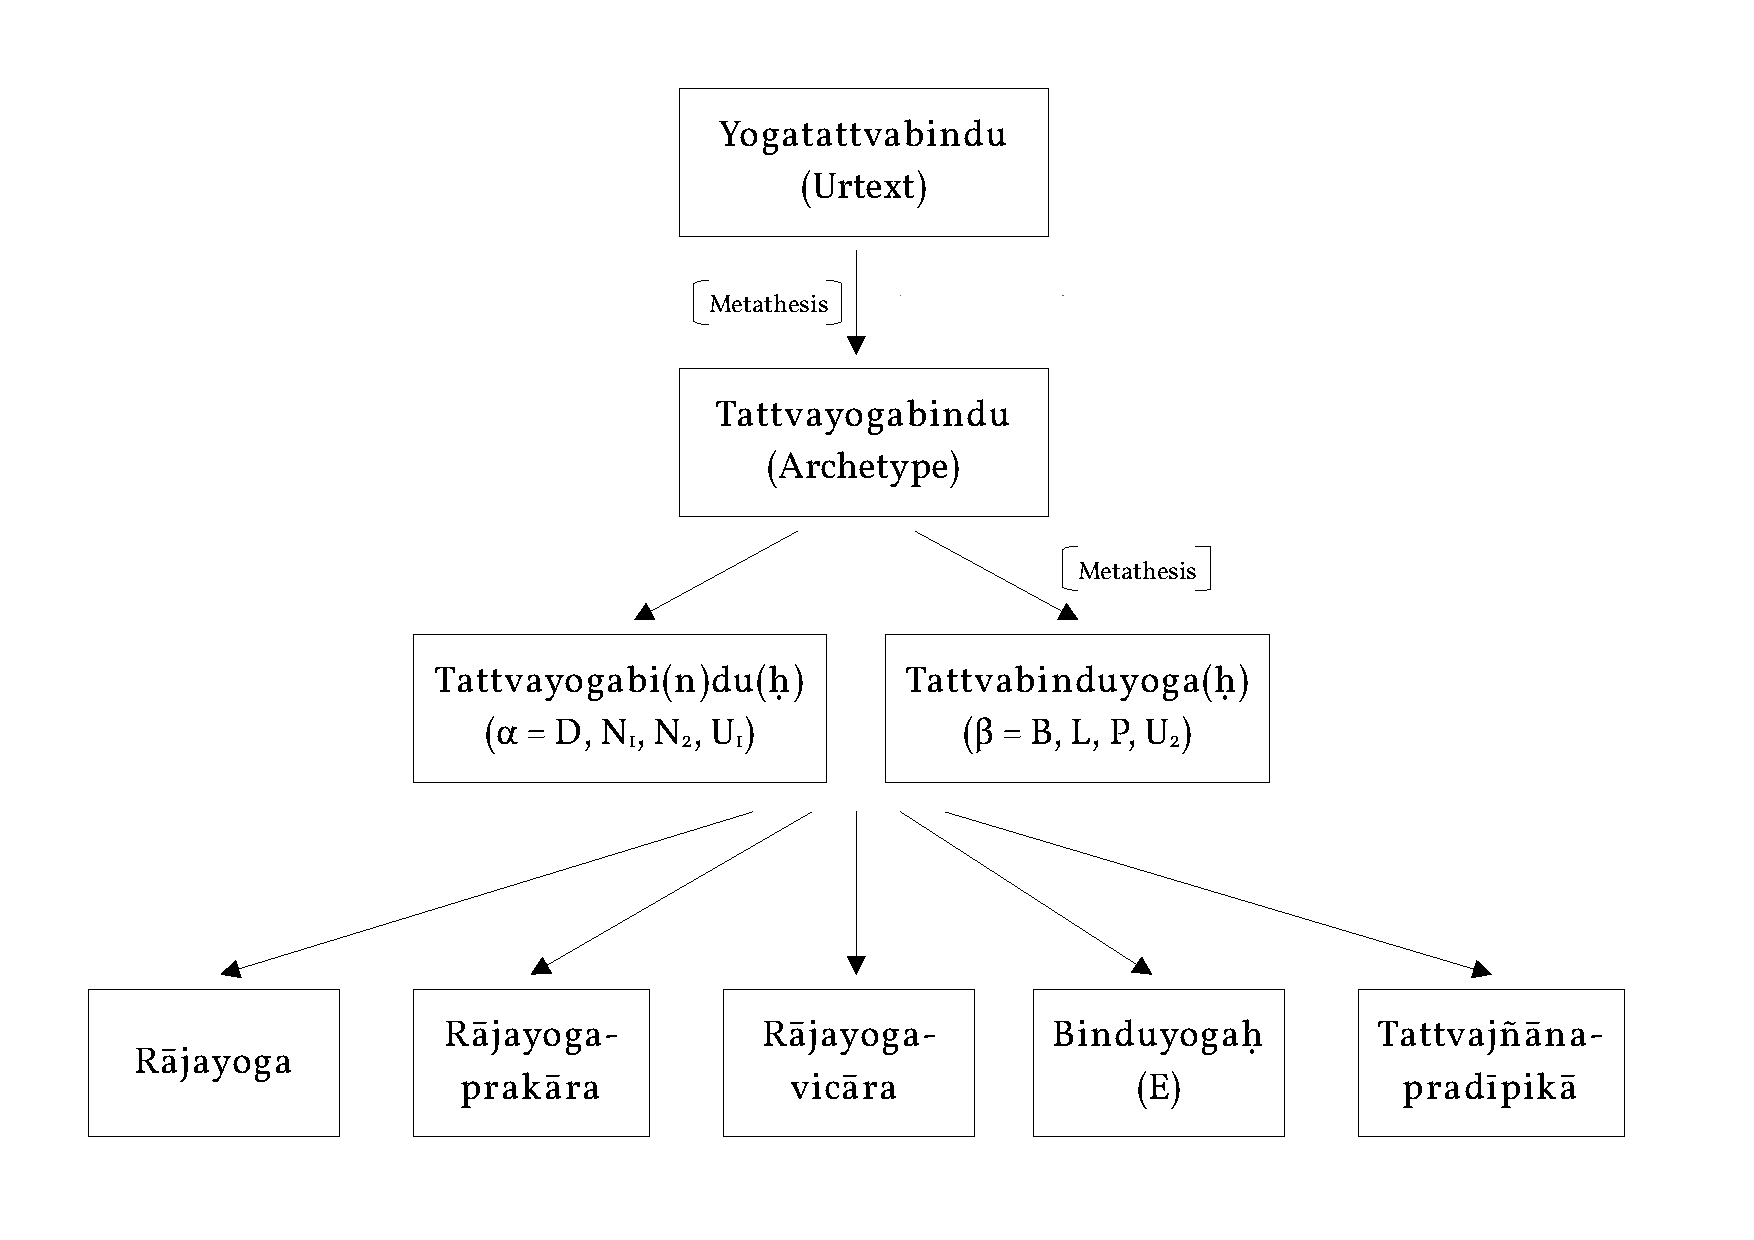
\includegraphics[width=1\textwidth]{pics/titel-hypothese.pdf} % Passe die Breite nach Bedarf an
    \caption{The hypothesis of the genesis of the transmission of the text's title.}
    \label{fig:titel-hypothese}
\end{figure}

\subsection{Description of the sources}

\subsubsection{Yogasvarodaya}

The \emph{Yogasvarodaya} (YSv) will be described in detail in the chapter ``Description of the sources''. Another treatment would be redundant.\footnote{See p. \pageref{yogasvarodayadescription}} The \emph{Yogasvarodaya} is a text known solely through quotations found in the \emph{Prāṇatoṣiṇī} and \emph{Yogakaṇikā}, which will be described below.

\subsubsection{Prāṇatoṣiṇī}

The \textit{Prāṇatoṣiṇī} (PT) by Rāmatoṣaṇa\footnote{Although the printed editions identify Rāmatoṣaṇa as the author of this work, sometimes bearing the titles Vidyālaṃkāra or Bhaṭṭācārya, \citeauthor{shastri1905} (1905: 2) mentions another name: ``Babu Prāṇakṛṣṇa Visvās of Khaṛhadaha, within ten miles of Calcutta, collected in the beginning of the nineteenth century a large number of Tantra, Purāṇa and Smṛti MSS., for the purpose of compiling Prāṇatoṣiṇī, Prāṇakṛṣṇā Kriyāmbudhi and other encyclopaedic works on Hindu ritual and worship.''

Since the \textit{Prāṇatoṣiṇī} is frequently cited in recent secondary literature on tantric studies but lacks detailed studies, critical editions, or complete translations into Western languages, this discrepancy remains unresolved.} is a Tantra compendium (\textit{nibandha}) from the 19th century, compiled by the author in Bengal. This extensive compendium addresses creation, the four \textit{puruṣārthas}, and devotion. The \textit{Prāṇatoṣiṇī} is divided into six major \textit{kāṇḍa}s (``sections''): 1. \textit{sargakāṇḍa} (subject: the creation of the universe and cosmogony), 2. \textit{dharmakhaṇḍa} (subject: rituals and Dharma of the twice-born), 3. \textit{arthakāṇḍa} (subject: daily routine, deity worship, purification practices, rites, offerings, etc.), 4. \textit{kāmyakāṇḍa} (subject: wish-fulfilment practices, protective mantras, etc.), 5. \textit{bhaktikāṇḍa} (subject: performance of devotional deity worship), and 6. \textit{jñānakāṇḍa} (subject: Mokṣa, Yoga, etc.). The author draws from a multitude of texts circulating in this region during the 19th century.

Additional topics of the \textit{Prāṇatoṣiṇī} range from \textit{mantras}, \textit{yantras}, and their meanings\footnote{See \citeauthor[2010: 69-70]{slouber2010}.} to meditations, religious stories, legends, and deity worship,\footnote{See \citeauthor[1997: 149-150]{kinsley1997}.} the six acts of magic, tantric rituals including sexual rites, and various areas of tantric philosophy.\footnote{See \citeauthor[2010: 100]{urban2010}.}

The \textit{Prāṇatoṣiṇī} incorporates a total of 304 verses from the \textit{Yogasvarodaya} in its \textit{jñānakāṇḍa}.\footnote{\emph{Prāṇatoṣiṇī}, 1898: 831-848.} All verses are cited with the reference \textit{yogasvarodaye}. These verses are quoted in a largely coherent sequence, giving the reader the impression of having the complete transmission of the text. However, this is not the case. Many additional verses of the \emph{Yogasvarodaya} can be found in the \emph{Yogakarṇikā} described below. There are numerous overlaps between the quotations. The main difference lies in the fact that, unlike the \textit{Prāṇatoṣiṇī}, the \emph{Yogakarṇikā} primarily includes practical instructions from the \textit{Yogasvarodaya}, such as instructions for \textit{prāṇāyāma}-, \textit{kumbhaka}-, or \textit{mudrā} techniques.

\subsubsection{Yogakaṇikā}

\subsubsection{Amarakośa}

\subsubsection{Siddhasiddhāntapaddhati}

\subsection{Description of the testimonia}

\subsubsection{Yogasaṃgraha}
\label{yogasamgraha}
\subsubsection{Haṭhasaṅketacandrikā}
\label{hathacandrika}
Hall S. 17 (catalogues) 

\subsection{Notes on the analogia}

\subsubsection{Amaraughaśāsana}
\subsubsection{Amanaska}

- Yogasiddhāntacandrikā
- Vivekamartanda
- yogabija
- yogacintamanu
- hathatattvakaumudi
- saubhagyalaksmiupanishad
- netratantra
- tantraloka
-manthanabharavatantra
- urmikaularnavatantra
- yogatarangini
- hathattatvakaumudi
- fausta 1967
- yogacudamani
- mandalabrahmaopanishad
- hathapradipika 

\section{Stemmatic analysis}
\label{stemma}
\footnote{Paolo Trovato and others explain the very high rate of lost archetypes and two-branched stemmata by ``the high (90\%) rate of extinction of individual copies'' \parencite[86]{trovato2017}.}

\section{Stylistic Particularities}

\section{Conventions for the critical edition}

\subsection{Guide to the apparatus}

\subsection{Conventions and Abbreviations}
\begin{itemize}
\item[Ed.] = Edition
\item[Ibid.] = Ibidem
\end{itemize}

\subsection{Sigla in the Critical Apparatus}

\begin{itemize}
\item E : Printed Edition
\item P : Pune BORI 664
\item L : Lalchand Research Library LRL5876
\item B : Bodleian Oxford D 4587
‚\item \None : NGMPP B 38-31
\item \Ntwo : NGMPP B 38-35 / A 1327-14
\item \Done : IGNCA 30019
\item \Uone : SORI 1574
\item \Utwo : SORI 6082
\end{itemize}



\chapter{Comparative analysis of the complex early modern Yoga taxonomies}
\label{yogas_list}
\label{yogatax}
\clearpage

%\section{The texts of the complex Yoga taxonomies}

%\subsection{Yogasiddhāntacandrikā}

%Versucht alle 15 Yogas im Samādhipāda des Pātañjalayogaśāstra unterzubringen.
%Siehe auch Powell 2023. 

%The Yogasiddhāntacandrikā is an ambitious work that attempts to unify a vast array of doctrines within the
%framework of the Yogasūtras of Patañjali. In particular, Nārāyaṇatīrtha attempts to synthesize fifteen
%different systems of yoga within the first chapter (pāda). All of these are believed to result in the state of
%Rājayoga, which Nārāyaṇatīrtha understands as synonymous with the nididhyāsana of Vedānta and
%the asaṃprajñātasamādhi of Pātañjalayoga.111


%\section{Comparative analysis of the complex Yoga taxonomies}
%\label{yogatax}

%%%%%%
%%%%%%hier adden das man sich von Rāmacandra gewünscht hätte, eine enzyklopädische Abhandlung der fünfzehn Yogas vorzufinden. Leider enttäuscht, strukturelle Probleme, bla bla ... aus diesem Grund "if you see a job its yours" 
%%%%%%
%%%%%%
\noindent
\lettrine[lines=2, lhang=0.2, loversize=0.25]{T}{he} similarities between the Yoga taxonomies of Rāmacandra's \textit{Yogatattvabindu}, his source text, the \textit{Yogasvarodaya} as well as the taxonomies laid out by Nārāyaṇatīrtha in his \textit{Yogasiddhāntacandrikā} and Sundardās' \textit{Sarvāṅgayogadīpikā} which all emerged within the 17th century have been initially observed and discussed briefly by \citeauthor{birch2014} (2014).\footnote{See \citeauthor[2014: 415-416]{birch2014}.} I would like to call this specific literary phenomenon the ``complex early modern Yoga taxonomies of the medieval Yogas'' or simply ``complex Yoga taxonomies''.

\begin{table}[H]
    \centering
    \begin{tabularx}{\textwidth}{>{\raggedright\arraybackslash}p{0.05\textwidth}XXXX}
        \toprule
        No. & \textit{Yogatattvabindu} & \textit{Yogasvarodaya} & \textit{Yogasiddhāntacandrikā} & \textit{Sarvāṅgayogadīpikā} \\
        \midrule
        1. & \textit{kriyāyoga} & \textit{kriyāyoga} & \textit{kriyāyoga} & \textit{\textbf{bhaktiyoga}} \\
        2. & \textit{jñānayoga} & \textit{jñānayoga} & \textit{caryāyoga} & \textit{mantrayoga} \\
        3. & \textit{caryāyoga} & \textit{karmayoga} & \textit{karmayoga} & \textit{layayoga} \\
        4. & \textit{haṭhayoga} & \textit{haṭhayoga} & \textit{haṭhayoga} & \textit{carcāyoga} \\
        5. & \textit{karmayoga} & \textit{dhyānayoga} & \textit{mantrayoga} & \textit{\textbf{haṭhayoga}} \\
        6. & \textit{layayoga}  & \textit{mantrayoga} & \textit{jñānayoga} & \textit{rājayoga} \\
        7. & \textit{dhyānayoga} & \textit{urayoga}   & \textit{advaitayoga} & \textit{lakṣayoga} \\
        8. & \textit{mantrayoga} & \textit{vāsanāyoga} & \textit{lakṣyayoga} & \textit{aṣṭāṅgayoga} \\
        9. & \textit{lakṣyayoga} & -                   & \textit{brahmayoga} & \textit{\textbf{sāṃkhyayoga}} \\
        10. & \textit{vāsanāyoga} & -                   & \textit{śivayoga} & \textit{jñānayoga} \\
        11. & \textit{śivayoga} & -                    & \textit{siddhiyoga} & \textit{brahmayoga} \\
        12. & \textit{brahmayoga} & -                  & \textit{vāsanāyoga} & \textit{advaitayoga} \\
        13. & \textit{advaitayoga} & -                 & \textit{layayoga} & - \\
        14. & \textit{siddhayoga} & -                  & \textit{dhyānayoga} & - \\
        15. & \textit{rājayoga} & - [\textit{rājayoga}]& \textit{premabhaktiyoga} & - \\
        16. & - & - & [\textit{rājayoga}] & - \\
        \bottomrule
    \end{tabularx}
    \caption{Comparative table of the four complex Yoga taxonomies 17th century}
    \label{tab:complextaxonomies}
\end{table}

The phenomenon of complex Yoga taxonomies raises various questions.
\begin{enumerate}
\item How are the individual Yoga categories used and classified in the four texts?
  \item Do the four texts use and understand the single Yogas in the same way, or are there differences?
  \item Furthermore, what conclusions can be drawn from answering the previous question in terms of the individual Yoga category and in the context of each text?
  \item Is there a direct historical connection between all the texts with complex Yoga taxonomies, or did they all arise independently?
  \item How can the phenomenon of ``complex early modern Yoga taxonomies of the medieval Yogas'' be situated within the broader context of the history of Yoga?
  \item Is it possible to explain why they did emerge? 
\end{enumerate}

To answer or at least approach these questions, the complex Yoga taxonomies and their single categories of Yoga are examined within a comparative analysis. The results will be linked with the recent findings of Yoga research.

This chapter will conduct an empirical comparative grounded in the hermeneutics of difference.\footnote{The term ``hermeneutics of difference'' should be understood in the context of the German concept ``Differenzhermeneutik'' as employed by the culturally oriented Heidelberg School of Religious Studies. Here, Differenzhermeneutik refers to an interpretative method, particularly in the comparative study of religions, that seeks to understand and analyze the diversity and distinctiveness of religious expressions. This approach emphasizes the context, cultural background, and the differences that shape a religious phenomenon. Instead of searching for universal principles, the focus is on the differences between various religious traditions and practices. Religious phenomena are examined within their specific cultural, historical, and social contexts, thus revealing the particular conditions and circumstances, as well as the internal logic and significance in their emic context, as viewed from an etic perspective. This etic perspective is critically reflected upon, so that the biases and assumptions of the researcher are taken into account. Researchers are encouraged to become aware of their own cultural and religious perspectives and to reflect on their impact on the understanding process.} It first historicizes the objects of comparison—the early modern Yoga texts \emph{Yogatattvabindu}, \emph{Yogasvarodaya}, \emph{Yogasiddhāntacandrikā}, and \emph{Sarvāṅgayogapradīpikā}—by placing them in their specific historical and religious contexts. It then instrumentalizes the empirically derived concept of ``complex early modern Yoga taxonomies of the medieval Yogas''\footnote{The metalinguistic capturing of this phenomenon, which appears in the mentioned texts, serves to delineate a specific religious-historical phenomenon observed in the 17th century on the Indian subcontinent in certain Yoga texts written in Sanskrit and Brājbhāṣa from different traditions. In this comparative study, it serves as the \textit{tertium comparationis}. ``Complex'' refers to a double-digit number of different Yoga categories in an early modern Yoga text, compared to the more widespread, less complex medieval Yoga taxonomies that describe a single-digit number of Yogas.} for the intended comparison. This aims to capture the structural and functional similarities and differences between the complex Yoga taxonomies and the individual Yoga taxa, considering the specific signatures of the texts. The results derived from this will be applied to the questions mentioned above.

The comparison will broaden and clarify our understanding of the respective spectrum of meanings of the individual Yoga categories in the discursive field of the authors of the texts containing the taxonomies. Furthermore, the comparison results in the documentation of the discursive web\footnote{Spoiler alert: There are astonishing differences!} of word usage of various Yoga categories in the 17th century. Additionally, contrasting the single Yoga categories used across traditions will sharpen our understanding of the categories themselves, as multiperspectivity will naturally reveal new aspects previously hidden to the eye. Individual Yoga categories that do not appear in the list of the \textit{Yogatattvabindu} but are listed in the other texts with complex taxonomies will also be covered and outlined. In addition, Yoga categories that do not appear in any of the analysed lists but are nevertheless mentioned in the texts will also be covered. Thus, this comparative study will display the overall picture of all Yoga categories used during the period under consideration in an encyclopedic fashion and will serve scholars as a comprehensive reference. However, it is essential to emphasise that the comparison of Yoga categories is limited to those texts that contain the complex Yoga taxonomies. Although the analysis and comparison of the Yoga categories can be extended to other Yoga texts, locations, and periods if necessary or valuable, for example, to provide the required context, the restriction on the complex Yoga taxonomies is generally maintained to prevent this complex endeavour from going \textit{ad absurdum}.\footnote{The historical tracing and analysis of developments in the reception history of the Yoga categories presented in the complex taxonomies can be used to generate valuable insights, as I have demonstrated by the example of the development of the early modern forms of Kriyāyoga into the modern forms of Kriyāyoga, beginning with the lineage of the world-famous Paramahaṃsa Yogānanda due to personal interest. See the chapter \textit{Excursus: Popularisation of a new Kriyāyoga in a global context} on p.\pageref{excursus} et seqq. Unfortunately, this example made me realise that it is beyond this work's scope to extend this analysis to the history of the reception of each Yoga category and term throughout the entire history of Yoga, particularly the transition from the early modern to the modern period. Fortunately, other scholars have already done great work in the last decade. A groundbreaking example of the history of Rājayoga is \citeauthor{birch2014} (2014), \citetitle{birch2014}. Even single yogic techniques can be extremely complex. For an outstanding article on the history of the haṭhayogic \textit{vajrolīmudrā} see for example \citeauthor{mallinson2018vajrolimudra} (2018), \citetitle{mallinson2018vajrolimudra}.} Ultimately, the comparative analysis of the texts, the authors and their multiple Yoga categories will help to formulate a new concise hypothesis as to why and under what circumstances the complex Yoga taxonomies emerged across traditions and largely independently of each other.

In striving to avoid the issues highlighted by Jonathan Z. \citeauthor{smith1982} in his revolutionary essay for the theoretical development of comparative religious studies titled \textit{In Comparison a Magic Dwells} (1982),\footnote{\citeauthor[1982]{smith1982}.} this work fundamentally follows the approach and methodology of Barbara A. \citeauthor{holdrege1994}. Her comparative model, presented in her essay \textit{Comparative Religion with a Difference} (1994), effectively addresses all the problems of comparative work criticized by Smith.\footnote{Cf. \citeauthor[1994: 804-805]{holdrege1994}.} This work adheres to her method, undergoing modifications tailored to this study in its three phases of analysis.\footnote{Cf. ibid. 1994: 806-812.} These phases are:
\begin{enumerate}
\item Historical-religious\footnote{The originally termed historical-cultural contextualization and content characterization is adapted here to historical-religious contextualization and content characterization, as this study deals with texts from the same culture but belonging to different religious streams within that culture. The specific tradition from which each text emerges is highly relevant to this comparative study.} contextualization and content characterization. Holdrege's first step, the ``Historical Interpretation,'' is adjusted to suit the present topic. In this first step, the comparative objects, i.e., the individual texts, are embedded in their historical and religious contexts, providing an overview of the significant contents. The primary focus is on the individual taxa of the Yoga taxonomies in the four texts. The necessary concepts and complexes of ideas for an adequate description and an immanent understanding of the Yoga category in each text are considered here. That will be achieved by analysing each individual Yoga of each individual text separately.  

\item The comparative analysis. Here, the differences and similarities of the ``complex early modern Yoga taxonomies of the medieval Yogas'' for each taxon will be highlighted. Within this framework, the constitutive concepts of each text and their tradition, which form the basis for each complex Yoga taxonomy, are contrasted.

\item The interpretation of the results. In this final step, the results are applied to the questions posed in the introduction. The significance of the differences and similarities is examined and reflected upon in the context of the introductory questions. That is initially done at the level of individual Yogas and finally at the overarching level, considering the results of the comparative analysis phase of all individual Yogas.
\end{enumerate}

In summary, this means the following: After describing and contextualising the four texts, the three analysis phases will be conducted for each Yoga category mentioned in these texts. The comparative analysis will follow the structure of the individual Yogas (the taxa) outlined in the \textit{Yogatattvabindu}. Each Yoga will initially be analysed in its context. The order is based on the order of the list in the \textit{Yogatattvabindu}. That is phase one. The results of the descriptions of each Yoga will be compared with each other. Some Yogas only appear in the taxonomies of \textit{Yogatattvabindu} and \textit{Yogasvarodaya} but are not explicitly dealt with in the text. At these points, reference is made to this fact, and the analysis is continued based on the explanations of the other taxonomies that describe these Yogas. Some Yogas only occur in one\footnote{In this case, a comparison is impossible. However, they are nonetheless described for an encyclopedic overview.} or two texts. They will be described, too, and compared if more than one text contains them. The third analysis phase is conducted for each Yoga category, which has more than one occurrence in the four texts. This part of the comparison will allow us to answer the questions 1-3 mentioned above. In a concluding step, an overarching third phase of analysis (the conclusion), the overall results of the analysis of the individual Yoga categories are summarised, interpreted, and applied to this comparative study's remaining significant questions (4-6 mentioned above). 

\section{Contextualising the four texts with complex Yoga taxonomies}

This section describes the four texts that contain the four known complex Yoga taxonomies. The focus will be on characterizing the historical and religious background of the texts and their authors. Additionally, an overview of the contents will be presented, along with other relevant facts for this comparison. Finally, the role of the complex Yoga taxonomies within each respective text will be highlighted. The analysis of the individual Yogas in each text, which follows this section, is always conducted within the specific religious, historical, and social context of the respective text. 

\subsection{\emph{Yogatattvabindu}}

The \emph{Yogatattvabindu} has already been extensively contextualized and in the introduction of this dissertation und critically edited for the first time.\footnote{For a more detailed discussion of the \emph{Yogatattvabindu}, see p. \pageref{generalremarks}.} It has been established that the \emph{Yogatattvabindu} was composed before 1659\footnote{The dating of the \emph{Yogatattvabindu} is discussed on p. \pageref{dating}.} and that it was most likely written somewhere in northern India. Much about the author remains unknown. Rāmacandra Paramahaṃsa, the author of the \emph{Yogatattvabindu}, held the title \textit{paramahaṃsa}, suggesting his initiation as a Daśanāmī Saṃnyāsī. Despite the Śaiva roots of his \textit{sampradāya}, he propagated a religious universalism as an Advaita Vedāntin. As outlined in the chapter \textit{Rāmacandra's audience},\footnote{See p. \pageref{ytb-audience} et. seqq.} the \emph{Yogatattvabindu} was certainly aimed at affluent segments of the population. Due to numerous text-immanent statements, it is even plausible that this Yogaśāstra was composed at an unknown royal court to educate young princes. If this is true, we must assume that Rāmacandra was employed as a Yoga teacher at the royal court. At the very beginning of the text, a complete list of fifteen Yogas, presented as methods of Rājayoga, is provided.\footnote{See p. \pageref{intro} and especially Table \ref{tab:complextaxonomies} on p. \pageref{tab:complextaxonomies} for an overview.} Rāmacandra places Rājayoga at the top of the taxonomy to highlight its overarching position, presenting Rājayoga as a universal category encompassing all other Yoga methods. Rāmacandra presents the following taxonomy: 1. Kriyāyoga, 2. Jñānayoga, 3. Caryāyoga, 4. Haṭhayoga, 5. Karmayoga, 6. Layayoga, 7. Dhyānayoga, 8. Mantrayoga, 9. Lakṣyayoga, 10. Vāsanāyoga, 11. Śivayoga, 12. Brahmayoga, 13. Advaitayoga, 14. Siddhayoga, and 15. Rājayoga itself.    

\subsection{\emph{Yogasvarodaya}}
\label{yogasvarodayadescription}
The \emph{Yogasvarodaya} is a Sanskrit Yoga text of the Rājayoga genre with a distinct Śaiva orientation, which was possibly written in central or south India.\footnote{The \emph{Yogasvarodaya} mentions the rivers Godāvarī and Kāverī. I discuss the role of the rivers of the \emph{Yogasvarodaya}, \emph{Siddhasiddhāntapaddhati} and \emph{Yogasvarodaya} on p. \pageref{riversrivers}, n. \ref{riversrivers}.} 
As the \emph{Yogasvarodaya} was the primary source for the compilation of Rāmacandra's \emph{Yogatattvabindu}, the \textit{terminus ante quem} for this work can also be set at 1659 CE.\footnote{The dating of the \emph{Yogatattvabindu} is discussed on p.\pageref{dating}.} Manuscripts of this text have yet to be discovered. We know of its existence only from quotations in other texts. These include primarily the \emph{Prāṇatoṣiṇī}, which cites 304 verses and a half verse from the \emph{Yogasvarodaya} with reference (\textit{yogasvarodaye})\footnote{Cf. \emph{Prāṇatoṣiṇī} Ed. pp. 831-848.}. The \emph{Yogakaṛnikā} cites a total of 137 verses with reference (\textit{yogasvarodaye}) and at least four additional verses without reference.\footnote{The four verses without reference are found in the first chapter of the \emph{Yogakaṛnikā}. In this chapter, many verses are not attributed to any text. That is noteworthy since the author Nath Aghorānanda consistently attributes verses in all other chapters. Additional verses from the \emph{Yogasvarodaya} might be found here.} The \citetitle{shabdakalpadruma} (Ed. p. 501) quotes seven verses of the \emph{Yogasvarodaya} with reference (\textit{iti yogasvarodayaḥ}), which form its entry for the term \emph{haṭhayoga}. There are numerous correspondences between the verses from the \emph{Yogasvarodaya} quoted in the \emph{Prāṇatoṣiṇī} and the \emph{Yogakaṛnikā}. It is, however, very noticeable that many verses attributed to the \emph{Yogasvarodaya} in the \emph{Yogakaṛnikā} containing practical instructions for \textit{kumbhaka}s or purification techniques (\textit{karma}s) are not found in the quotations of the \emph{Prāṇatoṣiṇī}. These same verses are also absent in the \emph{Yogatattvabindu}.\footnote{This suggests the existence of different recensions of the \textit{Yogasvarodaya} - one shorter version without practical instructions for physical techniques and another including them. If this is the case, Rāmacandra used the former as the template for the \emph{Yogatattvabindu}.} The texts that quote the \emph{Yogasvarodaya} are good indicators that the \emph{Yogasvarodaya} circulated in India's north-east.\footnote{The \textit{Prāṇatoṣinī}, written near Calcutta, cf. \citeauthor{shastri1905} (1905). The origin of the \emph{Yogakarṇikā} is unknown. The only available printed edition of the \emph{Yogakarṇikā} by \citeauthor{yogakarnika} (2004) is based on a manuscript presumably from Benares, cf. \citeauthor{yogakarnika} 2004: \lowroman{6}. Radhakanta Deva (1784-1867) compiled the \citetitle{shabdakalpadruma} in Calcutta. Thus, it can be inferred that northeastern India was a significant area for the circulation of the \textit{Yogasvarodaya}.}

The \emph{Yogasvarodaya} was probably addressing non-celibate householders.\footnote{Cf. \citeauthor[2018: 201]{mallinson2018vajrolimudra}.} However, some quotations of the \emph{Yogasvarodaya}, particularly one in the \emph{Yogakaṛnikā}, suggests that the \emph{Yogasvarodaya} might have had enthusiastic ascetics among it is readers.\footnote{Based on an understanding of \textit{śaktināḍī} as a ``powerful channel'' or ``mighty intestine'', the inclusion of the practice described here may have been way too extreme for householders and could only be aimed an enthusiastic ascetic audience. That technique is called \textit{nāḍikṣālanam} and described in the \emph{Yogakaṛnikā} with reference to \textit{yogasvarodaye}. \emph{Yogakaṛnikā} 4.73-77 (Ed. pp. 58-59; \approx \citetitle{gherandasamhita} 1.21-24; \approx \citetitle{hathayogasamhita1921} 2.11-15) reads: \textit{nāḍīkṣālanam} | \textit{kākīmudrāṃ sādhayitvā pūrayed udaraṃ marut} (\textit{marutodaram} \citetitle{hathayogasamhita1921} 2.11) | \textit{dhārayed ardhaṃ yāmāntaṃ cālayed ardhavartmanā} || 73 || \textit{nābhilagnajale sthitvā śaktināḍīṃ visarjayet} | \textit{karābhyāṃ kṣālayen nāḍīṃ yāvan malavisarjanam} || 74 || \textit{tāvat prakṣālya nāḍīṃ ca udare veśayet punaḥ} || 75 || \textit{idaṃ prakṣālanaṃ gopyaṃ devānām api durlabham} || 76 || \textit{kevalaṃ dhautimātreṇa devadeho bhaved dhruvam} | \textit{yāmārddhaṃ dhāraṇāśaktiṃ yāvan no dhārayen naraḥ} | \textit{bahiṣkṛtaṃ mahādhautaṃ tāvan naiva ca kārayet} || 77 || ``(73) Having cultivated the crow-seal, fill the stomach with air, hold it for an hour and a half, then move by the midway [path]. (74) Standing in water up to the navel, draw out the mighty intestine \textit{śaktināḍī}. Wash out the intestine with both hands until all dirt is gone. (75) Having thoroughly washed the intestine, return it to the stomach. (76) This cleansing is so secret that even gods find it difficult to obtain. (77) By this cleansing alone, one certainly achieves the divine body. As long as a man is not able to hold the breath for an hour and a half, he is not capable of performing the externalised great wash (\textit{mahādhauta}).'' Further research revealed that this interpretation of \textit{śaktināḍī} is common among Indian scholars, as it is also found in \citeauthor{pureyoga} (1992: 46-47) and additionally in \citeauthor{sahai1972} (1972: 123). This is reinforced by a reading in \citetitle{hathayogasamhita1921} 2.11, which reads \textit{gudavartmanā} instead of \textit{ardhavartmanā} in the context of the preliminary practice called Kākīmudrā.}

Large parts of the content and the content's structure are similar to those of the \emph{Yogatattvabindu}, except for the few passages where Rāmacandra exclusively relies on the \emph{Siddhasiddhāntapaddhati}.\footnote{In particular, this concerns \textit{Yogatattvabindu} \uproman{43} on the topic of \textit{avadhūtapuruṣa}, as well as individual passages of cosmogony, such as sections \uproman{48}, \uproman{53}, \uproman{54}, \uproman{55}, \uproman{56}, and \uproman{57}.} Furthermore, only the quotations in the \emph{Yogakarṇikā} attest that the \emph{Yogasvarodaya} also taught various physical practices not present in the quotations of the \emph{Prāṇatoṣiṇī}: detailed description of the \textit{ṣaṭkarma}s (4.40-49, 4.67-80), \textit{kevalakumbhaka} and \textit{pratyāhāra} (6.23-34), instructions for \textit{kumbhaka} (7.1-10, 7.23-28, 7.67-72), and instruction on \textit{khecarimudrā} (8.136-141). Thus, we can assume that these descriptions were much more numerous in the original \emph{Yogasvarodaya}.

The \emph{Yogasvarodaya} presents the five Yogas immediately at the beginning of its text. The fifteen Yogas are understood, just like in the \emph{Yogatattvabindu}, as equivalent methods of Rājayoga. Of the total fifteen announced Yogas, only eight methods of Rājayoga are named in this introduction according to the quotation from the \emph{Prāṇatoṣiṇī}. \emph{Prāṇatoṣiṇī} (Ed. p. 831) reads:

\begin{quote}
  \textit{atha rājayogaḥ} || \textit{yogasvarodaye} | \\
  \textit{īśvara uvāca} |\\
  \textit{rājayogaṃ pravakṣyāmi śṛṇu sarvatra siddhidam} | \\
  \textit{guhyād guhyataraṃ devi nānādharmaṃ parāt param} || \\
  \textit{rājayogena deveśi nṛpapūjyo bhaven naraḥ} |\\
  \textit{rājayogī cirāyuś ca aṣṭaiśvaryamayo bhavet} || \\
  \textit{pañcadaśaprakāro'yaṃ rājayogaḥ} ||\\
  \textit{kriyāyogo jñānayogaḥ karmayogo haṭhas tathā} |\\
  \textit{dhyānayogo mantrayoga urayogaś ca vāsanā} |\\
  \textit{rājaty etad brahmavaśīva ebhiś ca pañcadaśadhā} |
\end{quote}
\begin{quote}
Now Rājayoga. [As described] in the Yogasvarodaya. 
God said: ``I will teach Rājayoga, listen! In every case, it bestows completion. 
[It is] more secret than secret, oh Goddess, [its] nature is manifold, [and it is] higher than the highest. 
By means of Rājayoga, oh Goddess, the person is to be praised like a king.
The Rājayogin may have a long life, and he may be equipped with the eight [supernatural] powers.
This Rājayoga has fifteen varieties:
Kriyāyoga, Jñānayoga, Karmayoga, Haṭha[yoga], 
Dhyānayoga, Mantrayoga, Urayoga and Vāsanā[yoga]. 
By [means of] these fifteen [yogas], this [person] who is resting in Brahman shines [like a king].''
\end{quote}

Not all of the eight Yogas mentioned in the introduction are explained in the course of the text. The Yogas treated in the text are: Kriyāyoga, Jñānayoga, Lakṣyayoga, which was not mentioned in the introductory verses, Rājayoga, Haṭhayoga, another form of Jñānayoga, and Aṣṭāṅgayoga, which was also not mentioned in the introduction. Since there is still no complete transmission of the \emph{Yogasvarodaya}, it remains uncertain whether the text ever contained a more comprehensive description of the Yogas.

\subsection{\emph{Yogasiddhāntacandrikā}}

The \emph{Yogasiddhāntacandrikā} is an important commentary on Patañjali's \emph{Yogasūtra}. Nārāyaṇatīrtha was a Brāhmaṇa, a devotee of Kṛṣṇa, a \textit{saṃnyāsa}, a renowned intellectual\footnote{Later authors like Brahmānanda considered Nārāyaṇatīrtha an authority in the field of yoga, as evidenced by his citation in the \citetitle{jyotsna} (Ed. p. 6).} and a prolific author\footnote{Nārāyaṇatīrtha composed several commentaries on the \emph{Yogsūtra} and other works in different literary genres. See \citeauthor[2004: 20-21]{penna2004}.} Studies suggest that Nārāyaṇatīrtha flourished between 1600 and 1699.\footnote{Cf. \citeauthor[1993: 56]{endo1993}.} Nārāyaṇatīrtha spent a considerable amount of time in Benares, though the exact period of his stay is unclear.\footnote{See especially \citeauthor[2004: 24]{penna2004}. A comprehensive study on the life and works of Nārāyaṇatīrtha can be found in Endo \citeauthor{endo1993}'s \citetitle{endo1993} (1993). All excerpts of the \emph{Yogasiddhāntacandrikā} used in this dissertation are based on the following edition: \fullcite{yogacandrika}.}
As \citeauthor{birch2014} (2014: 414) noted, in his \emph{Yogasiddhāntacandrikā}, Nārāyaṇatīrtha is likely the first author to integrate the teachings of Haṭhayoga with Pātañjalayoga.\footnote{The \emph{Yogasiddhāntacandrikā} is also the first text in the commentary tradition of Pātañjalayoga to document a proliferation of \textit{āsanas}. In his commentary on \emph{Yogasūtra} 2.46, Nārāyaṇatīrtha lists and describes a total of 38 \textit{āsanas}. A detailed discussion of Haṭhayoga in the \emph{Yogasiddhāntacandrikā} can be found on p. \pageref{hathacandrika} et. seqq.} At the beginning of his commentary (1.1), he even enumerates fifteen different Yogas, which he locates throughout his commentary, particularly in the first two chapters of the \emph{Yogasūtra}. These Yogas are as follows: Kriyāyoga, Caryāyoga, Karmayoga, Haṭhayoga, Mantrayoga, Jñānayoga, Advaitayoga, Lakṣyayoga, Brahmayoga, Śivayoga, Siddhiyoga, Vāsanāyoga, Layayoga, Dhyānayoga, and Premabhaktiyoga. Nārāyaṇatīrtha conceptualizes all fifteen Yogas as valid methods for achieving the overarching goal of Pātañjalayoga, namely \textit{asaṃprajñātasamādhi}, which he equates with Rājayoga in his commentary on 1.20.\footnote{See p. \pageref{rajacandrika} for the passages and a detailed discussion of Rājayoga in the \emph{Yogasiddhāntacandrikā}.}

\subsection{\emph{Sarvāṅgayogapradīpikā}}

Sant Sundardās (1596–1689) was a prominent 17th-century poet and scholar who, as a follower of the Dādūpanth, a religious group named after its founder Dādū, was deeply rooted in the Vaiṣṇava bhakti tradition.\footnote{For a comprehensive account of Dādū and the Dādūpanth (1544–1603), see \citeauthor[2023: 71–77]{horstmann2023shrine}.} Born in the Būsar line of the Khandelval merchant caste (\textit{Vaiśya}), Sundardās met Dādū at a young age, probably shortly before 1600, and became his disciple.\footnote{Cf. \citeauthor[2023: 86]{horstmann2023shrine}.}.

Together with other Dādūpanthīs, he studied from the age of eleven in Benares under the initial guidance of Jagīvandās, a Brāhmaṇa disciple of Dādū, who maintained an ashram near Sundardā's birthplace in Dausa. During this time, he mastered Sanskrit, poetry (\textit{kāvya}) and the prevailing knowledge systems of his time. Sundardās is recognised as the best educated Dādūpanthī of his time.

After completing his education, Sundardās moved to Fatehpur in Rajasthan. He was known as a Sant poet and wrote numerous works\footnote{A selection of Sundardās' works has been translated by \citeauthor{horstmann2023shrine} in the book \citetitle[2023: 151-182]{horstmann2023shrine}.}, and his scholarly activities extended to various disciplines.

Sundardās commissioned most of his works and transcribed them into a single manuscript in 1685 A.D., just a few years before he died in 1689. This manuscript, known as the \emph{Granthāvalī}, comprises three volumes, with the \emph{Sarvāṅgayogapradīpikā} in the second volume. This collection contains 38 texts of varying lengths dealing with topics such as \textit{jñāna}, Yoga, and the Guru.\footnote{Cf. \citeauthor[2014: 685]{burger2014sarvangayogapradipika}.}

The \emph{Sarvāṅgayogapradīpikā} or ``Light on the Yoga of all Limbs'', written in \textit{Brajbhāṣā}, is a seminal historical document that systematically categorises twelve different Yogas. Sundardā's text aims to present Yoga as a cohesive, progressive system and reflects his comprehensive understanding of the discipline, which has undoubtedly influenced many contemporary Sants.

The Yoga system in the \emph{Sarvāṅgayogapradīpikā} is divided into three main categories comprising twelve different Yogas. Each tetrad consists of four Yogas, including the main category which Sundardās presents as an individual Yoga itself.  The first main category is Bhaktiyoga (2.1-51), including Bhaktiyoga (2.1-15), Mantrayoga (2.16-27), Layayoga (2.28-39), and Carcāyoga (2.40-51). The second category is Haṭhayoga (3.1-52), consisting of Haṭhayoga (3.1-12), Rājayoga (3.13-24), Lakṣayoga (3.25-36), and Aṣṭāṅgayoga (3.37-52). The last category is Sāṃkhyayoga (4.1-50), which includes Sāṃkhyayoga (4.1-12), Jñānayoga (4.13-24), Brahmayoga (4.25-30) and Advaitayoga (4.31-50). Each Yoga is assigned approximately the same number of verses, with each main category receiving about fifty stanzas.

Sundardās' system emphasises the interconnectedness and complementarity of these Yogas, which all converge towards his ultimate goal of Advaitayoga, his system's final limb (\textit{aṅga}).  

Sundardās also describes practices that he rejects (1.12-49). He emphasises his disdain for the six philosophical schools (1.11). In other verses, he shows a strong anti-ritualistic attitude and mocks ritual practices, ascetic performances, Jain rites and quacks. He criticises groups such as the \textit{kāpālikā}s, \textit{paśupata}s and other ascetics and denounces their extreme behaviour.\footnote{For example, Sundardās writes in \emph{Sarvāṅgayogapradīpikā} 1.34 Sundardās writes: 
\textit{kecit kaṃda mūla khani khāhīṃ, ekāeka rahaiṃ bana māhīṃ} \textit{kecit kāsāyadika pahiraiṃ, japahiṃ jāpa paiṭhahiṃ jala gaharaiṃ}|| ``Some dig up roots and bulbs and eat them, and live alone in the forest. Others wear saffron robes, recite mantras and sit in deep water.'' Similarly, in \emph{Sarvāṅgayogapradīpikā} 1.40, he remarks: \textit{kecit meghāḍambara baiṭhaiṃ, śīta kāla jalasāī paiṭhaiṃ} | \textit{kecit dhūma pāna kari bhūlaiṃ, auṃdhe hoi bṛccha sauṃ jhūlaiṃ} || ``Some sit on mountain peaks like clouds, in the cold season they lie in the water. Some breath smoke [and] digress, [some are] hanging upside down from trees.''} He never explains the practices of the latter groups as Yogas but as doctrines (\textit{mata}s).

Sundardās recognises and distances himself from what he considers heretical and glorifies the teachings of his master, Dādū. His adoration for the Guru is evident in his writings, which are imbued with personal devotion.

\section{Comparison of the individual Yoga categories in the four texts of the compley Yoga taxonomies}

We have observed that although the complex Yoga taxonomies are situated in very different texts and religious contexts, they show remarkable similarities. As previously announced, the individual Yoga categories of the four Yoga taxonomies will be compared in the following section. This comparison will elucidate the spectrum of meanings of the individual Yoga categories, expanding our understanding of the discursive web of negotiations surrounding these yogas in the 17th century. The contrast of the individual yoga categories across traditions will sharpen our understanding of the categories themselves.

\section{Kriyāyoga}

Kriyāyoga, ``the Yoga of action'', is the first method of Rājayoga within the list of fifteen Yogas presented by Rāmacandra and his source text \textit{Yogasvarodaya}. Remarkably, Nārāyaṇatīrtha also positions Kriyāyoga at the first position within the list of fifteen Yogas in his \textit{Yogasiddhāntacandrikā}. Sundardās, on the other hand, omits Kriyāyoga altogether. 

\subsection{Kriyāyoga in the \textit{Yogatattvabindu}}
\label{kriyaintro}
Since Rāmacandra refers to all fifteen Yogas as variants of Rājayoga in his initial definition of Yoga, and no explicit hierarchy is recognisable from his formulations in the text, all variants of Rājayoga appear to have been regarded by him as equally effective. All Yogas aim towards the same goal: long-term durability of the body (\textit{bahutarakālaṃ śarīrasthitiḥ}). The positioning of Kriyāyoga does not initially provide any information about the efficiency or the assignment of differently talented practitioners to a particular type of Yoga, as was the case in i.e. the widespread fourfold taxonomies.\footnote{According to \citetitle{amaraugha2024}\textit{prabodha} 18-24, Mantrayoga is best suited for the weak, Layayoga for the average, Haṭhayoga for the talented and Rājayoga for the exceptionally talented practitioner. In \citetitle{datta2024} 14, one finds the statement that the lowest practitioner should perform Mantrayoga, which is then also referred to as the lowest Yoga. \citetitle{mallinson2007} 12-28 expands this fourfold scheme of Yogas and practitioners with a temporal dimension. The weak practitioner needs twelve years to succeed with Mantrayoga, the average practitioner needs eight years with Laya, the able practitioner six years with Haṭha and the exceptional practitioner three years with Rājayoga.} Implicit hierarchical aspects are nevertheless present - although all Yoga types are a type of Rājayoga, Rāmacandra nonetheless places Rājayoga in the final and topmost position of his taxonomy.
The only apparent reason why Rāmacandra specifies Kriyāyoga as the first Yoga seems to be that his primary source text, whose content structure he largely follows, specifies this type of Yoga as the first.

The passage on Kriyāyoga in the \textit{Yogatattvabindu} is relatively short. The four verses presented by Rāmacandra are quoted without attribution from the \textit{Yogasvarodaya}. A prose section repeats the content of the verses. By definition, Kriyāyoga in the \textit{Yogatattvabindu} is ``liberation through [mental] action'' (\textit{kriyāmuktir ayaṃ yogaḥ}). In contrast to Rāmacandra's worldly definition of Rājayoga and its subcategories, here, liberation (\textit{mukti}) overrides this initial goal. In addition, the practitioner achieves ``success in one's own body'' (\textit{svapiṇḍe siddhidāyakaḥ}). The method of Kriyāyoga involves restraining any [mental] wave before an action. This restraint consists of reducing negative [mind-]waves and cultivating positive ones. Noticeably, the number of negative waves significantly exceeds the number of positive waves.

\begin{table}[H]
    \centering
    \begin{tabularx}{\textwidth}{XX}
        \toprule
        \textbf{Mental waves to be cultivated} & \textbf{Mental waves to be reduced} \\
        \midrule
        Patience (\textit{kṣamā}) & Envy (\textit{matsārya}) \\
        Discrimination (\textit{viveka}) & Selfishness(\textit{mamatā})\\
        Equanimity (\textit{vairāgya}) & Cheating (\textit{māyā})\\
        Peace (\textit{śānti}) & Violence (\textit{hiṃsā})\\
        Modesty (\textit{santoṣa}) & Intoxication (\textit{mada})\\
        Desirelessness (\textit{niṣpṛha}) & Pride (\textit{garvata})\\
        & Lust (\textit{kāma}) \\
        & Anger (\textit{krodha}) \\
        & Fear (\textit{bhaya})\\
        & Laziness (\textit{lajjā})\\
        & Greed (\textit{lobha})\\
        & Error (\textit{moha})\\
        & Impurity (\textit{aśuci})\\
        & Attachment and aversion (\textit{rāgadveśau}) \\
        & Disgust and laziness (\textit{ghṛṇālasya})\\
        & error (\textit{bhrānti})\\
        & Deceit (\textit{daṃbha})\\
        & Envy (repeatedly) (\textit{akṣama})\\
        & Confusion (\textit{bhrama})\\
        \bottomrule
    \end{tabularx}
    \caption{Mental waves to be cultivated and reduced in Rāmacandra's Kriyāyoga}
    \label{tab:waves}
\end{table}

The one who cultivates positive [mind-]waves and reduces the negative is called a \textit{kriyāyogī}. In the prose passage of the section, the term \textit{bahukriyāyogi} is used. The term is unprecedented in the rest of Yoga literature and presumably intends to express the great amount of reduced and cultivated [mind-]waves.\footnote{Cf. section \uproman{2} of the \textit{Yogatattvabindu} for its text on the subject Kriyāyoga.} 

\subsection{Kriyāyoga in the \textit{Yogasvarodaya}}
A closer examination of the Kriyāyoga section in the \textit{Yogasvarodaya} reveals Rāmancandra's reductionism since he excludes significant aspects of the original concept of the \textit{Yogasvarodaya}'s Kriyāyoga.

%YK 1.214-216

\begin{quote}
  \begin{ekdosis}
\textit{dhyānapūjādānayajñajapahomādikāḥ kriyāḥ} |\\
\textit{kriyāmuktimayo yogaḥ\app{\lem[wit={YTB}]{svapiṇḍe siddhidāyakaḥ}
  \rdg[wit={PT}]{sapiṇḍisiddhidāyakaḥ}
  \rdg[wit={YK}]{sapiṇḍisiddhidāyakaḥ}}} || 1 ||

(1) Actions are meditation, ritual veneration, donation, recitation, fire sacrifice, etc. 
The Yoga made of liberation through action[s] bestows success in one's own body. 

\textit{yat karomīti saṅkalpaṃ kāryārambhe manaḥ sadā} |\\
\textit{tat sāṅgācaraṇaṃ kurvan kriyāyogarato bhavet} || 2 ||

(2) When the mind, when starting an activity, performs the definite intention ``I am acting''
together with its auxilliaries, then one is devoted to Kriyāyoga. 

\textit{kṣamāvivekavairāgyaśāntisantoṣanispṛhāḥ} |\\
\textit{etad yuktiyuto yo 'sau kriyāyogo nigadyate} || 3 ||

(3) Patience, discrimination, equanimity, peace, modesty, desirelessness:
The one endowed with these means is said to be a Kriyāyogī.

\textit{mātsaryaṃ mamatā māyā hiṃsā ca madagarvitā} |\\
\textit{kāmaḥ krodho bhayaṃ lajjā lobho mohas tathā 'śuciḥ} || 4 ||

(4) Envy, selfishness, cheating, violence, intoxication and pride,
lust, anger, fear, laziness, greed, error, and impurity.

\textit{rāgadveṣau ghṛṇālasyaśrāntidambhakṣamābhramāḥ} |\\
\textit{yasyaitāni na vidyante kriyāyogī sa ucyate} || 5 ||

(5) Attachment and aversion, disgust and laziness, error, deceit, envy [and] confusion:
Whoever does not experience these is called a Kriyāyogī.

\textit{sa eva muktaḥ sa jñānī caṇḍināśena īśvaraḥ} |\\
\textit{kriyāmuktikaro yo'sau rājayogaḥ sa muktidaḥ} || 6 || (om. YK)

(6) He alone, the wise one, the lord, through the destruction of impetuous [behaviour]
who performs the liberation through action[s] is liberated. This Rājayoga is the bestower of liberation.

\textit{yāvan mano layaṃ yāti kṛṣṇe svātmani cinmaye} | \\ 
\textit{bhaved iṣṭamanā mantrī japahomau samabhyaset} || 7 ||\footnote{7ab \approx \citetitle{rudrayamala1937} 38.58cd.} (om. YSv) 

(7) Until the mind enters absorption into Kṛṣṇa, in one's own self, into consciousness,
the mantra practitioner (\textit{mantrin}) should practise recitation and fire sacrifice with an aspiring mind. 

\textit{vidite paratattve tu samastair niyamair alam} |\\
\textit{tālavṛntena kiṃ kāryaṃ lavdhe malayamārute} || 8 ||\footnote{\approx \citetitle{kularnavatantra} 9.28 \& \citetitle{yuktabhavadeva} 1.80.} (om. YSv) 

(8) When the highest principle has been realised through all the \textit {niyama}s, as is proper,
why should one wave the palm frond when the wind from the Himalayas has already reached?

\textit{tāvat karmmāṇi kurvanti yāvajjñānaṃ na vidyate} |\\ 
\textit{jñāne jāte pareśāni karmākarma na vidyate} || 9 || (om. YSv) 

(9) As long as [regular?] actions are performed, so long realisation is unknown.
When knowledge ensues, oh, Supreme Goddess, neither action nor non-action is known.
\end{ekdosis}
\end{quote}

These verses\footnote{The numbering used here was introduced by me for practical reasons and does not correspond to the original numbering of the verses in the citations of the source texts. The \textit{Prāṇatoṣiṇī} does not number the verses at all. The verses can be found in the printed edition of the \textit{Prāṇatoṣiṇī} on p. 831. The verses here are in the \textit{Yogakarṇikā} with the numbering 1.209-216 and can be found in the edition on p. 17.} stem from the only two currently available sources of the \textit{Yogasvarodaya}, namely the quotations from the \textit{Prāṇatoṣiṇī}\footnote{A considerable part of the \textit{Yogasvarodaya} is quoted with source reference (\textit{yogasvarodaye}).} and the \textit{Yogakarṇikā}.\footnote{Normally the \textit{Yogakarṇikā} quotes its sources. This passage is one of the few exceptional cases in which the verses have been taken from the \textit{Yogasvarodaya} without citing the source. However, this passage ends after verse 1.216 with ``\textit{iti yogasaṅketāḥ} |''.} The quotations of both texts essentially correspond, but the last verses of the passage differ. It cannot be ruled out that the last three verses of the \textit{Yogakarṇikā} in particular come from a different source and were not present within the \textit{Yogasvarodaya}. However, their content is so closely interwoven with the preceding verses that this scenario can be considered unlikely.

The main difference to the Kriyāyoga that Rāmacandra has constructed from these verses is the definition of the actions (\textit{kriyāḥ}) mentioned immediately at the beginning of the verses, of which the actions (\textit{kriyā}s) of Kriyāyoga is then predominantly composed, namely of (1) meditation, (2) ritual worship of God, (3) offerings, (4) recitation and (5) fire sacrifice, etc. Furthermore, while Rāmacandra declares the elements mentioned in the table \ref{tab:waves} as waves (\textit{kallola}) of the mind which are either required to be cultivated or reduced before any action is executed, the same elements are conceptualised in the \textit{Yogasvarodaya} as the intentions (\textit{saṅkalpa}) preceding the previously defined actions (\textit{kriyā}s), which should be observed.

In the three verses concluding this section, which are only handed down in the \textit{Yogakarṇikā}, the practitioner is referred to as \textit{mantrin} and should perform recitation and fire offerings until entering absorption (\textit{laya}).

A possible historical link, particularly in front of the Vaiṣṇava background, is the model of Kriyāyoga as found in the \textit{Uddhavagīta}\footnote{See i.e., \citeauthor[2007]{uddhavagita2007}.} which is a part of the famous \textit{Bhāgavatapurāṇa}\footnote{See i.e., \citeauthor[1950]{bhagavata}.}. Here, in chapter XXII.1-55 Kṛṣṇa describes a Vaiṣṇava form of Kriyāyoga in response to a request by his disciple Uddhava. The practice entails a very complex and devotional ceremonial veneration of the deity through offerings such as flowers and food, accompanied by the recitation of prescribed mantras, meditation, and the ritual consecration of the deity, among other rites. According to the text, this type of Yoga is the most beneficial for women and the working class (22.4) and is considered a means for liberation from the fetters of Karma (22.5). The Kriyāyoga described here is presented to be in line with both the Vedas and the Tantras, considering enjoyment (\textit{bhukti}) and liberation (\textit{mukti}) and is promised to bestow perfection in both this life and the next, by the Lord's grace (22.49).  

Furthermore, this concept of Kriyāyoga in the \textit{Yogasvarodaya} might be linked to the \textit{kriyāpāda}\footnote{See e.g. \citeauthor{ganesan2016saiva} (2016) and \citetitle{mrgendragama} (1962), Ed. pp. 1-205.} of the Śaiva \textit{āgama}s. The Śaiva \textit{āgama}s are collections of various tantric traditions, written in Sanskrit or Tamil, in which cosmology, epistemology, philosophical teachings, various practices such as meditation or Yoga, mantra recitation, worship of the gods, etc. are described. These texts\footnote{The fourfold division of \textit{pāda}s is only present in a limited number of Āgamas: \textit{Kiraṇa}, \textit{Suprabheda}, \textit{Mṛgendra} and \textit{Mataṅgaparameśvara} (as Upāgamas), see \citeauthor[1993: 225-461]{brunner1994place} for an overview.} usually consist of four sections (\textit{pāda}s): The \textit{jñānapāda} (knowledge section), \textit{kriyāpāda} (action section), \textit{caryāpāda} (behaviour section) and the \textit{yogapāda} (yoga section).\footnote{The order or the \textit{pāda}s varies, but the \textit{yogapāda} is always at the final position.} It can be no coincidence that \textit{jñāna°}, \textit{kriyā°} and \textit{caryā°} were each integrated as a separate Yoga category within the taxonomy of the fifteen Yogas\footnote{see p.\pageref{intro}.}. The \textit{kriyāpāda} is the section of a Śaiva \textit{āgama} that describes rules and practices for the performance of various rituals such as the significant initiation (\textit{dīkṣa}), ceremonies and worship of the gods. Additionally, \textit{prāṇāyāma} techniques and meditations are often found as parts of these rituals. There are also explanations of the nature of \textit{mudrā}s, \textit{maṇḍala}s and \textit{mantra}s. Furthermore, various characteristics of different types of Śaiva initiates\footnote{These are \textit{samayin, putraka, sādhaka, ācārya,} and \textit{astrābhiṣeka}.} can be found here.\footnote{See \citeauthor{ganesan2016saiva} (2016) for a general overview of the four \textit{pāda}s. One of the few Śaiva \textit{āgama}s that has been edited and translated into a Western language (French) is the \citetitle{mrgendragama}. For this see \citeauthor{mrgendragama}'s \citetitle{mrgendragama} (1962) \& \citeauthor{mrgendragamabrunner}'s \citetitle{mrgendragamabrunner} (1985).} The \textit{kriyā}s mentioned at the beginning of the \textit{Yogasvarodaya} - meditation, ritual veneration, donation, recitation, fire sacrifice, etc. have hardly deniable parallels to the \textit{kriyāpāda}s of the Śaiva \textit{āgama}s and thus could have their reception-historical roots precisely there. The other part, however, which describes the cultivation or reduction of certain mental configurations preceding all actions (\textit{saṅkalpa}) or [mental] waves (\textit{kallola}), I have not yet been able to locate in the Śaiva \textit{āgama}s, but they seem to be a simplyfied rendering of the Pātañjalean model of Kriyāyoga that was passend on in hitherto unknown traditions that practiced this type of Kriyāyoga.

\subsection{Kriyāyoga in the \textit{Yogasiddhāntacandrikā}}

The Kriyāyoga in Nārāyaṇatīrtha's commentary on \textit{Pātañjalayogaśāstra} entitled \textit{Yogasiddhāntacandrikā} presents Kriyāyoga as the first of his fifteen Yogas, which he locates in Pātañjalayoga.\footnote{For an earlier brief discussion of Kriyāyoga in Nārāyaṇatīrtha's \citetitle{yogacandrika} see \citeauthor[2004: 62-66]{penna2004}.} The term Kriyāyoga occurs in \textit{Pātañjalayogaśāstra} 2.1. According to the introduction to this \textit{sūtra}, in the \textit{bhāṣya}-part of the \textit{Pātañjalayogaśāstra}, Kriyāyoga is the means by which someone with a distracted mind can also attain Yoga (\textit{vyutthitacitto 'pi yogayuktaḥ}). In \citetitle{yogasutra} 2.1, Kriyāyoga is defined as follows:
\begin{quote}  
  \textit{tapaḥsvādhyāyeśvarapraṇidhānāni kriyāyogaḥ} |
\end{quote}
\begin{quote}
The Yoga of action consists of auterity, the self-study and devotion to the supreme lord. 
\end{quote}

Kriyāyoga, or ``yoga of action'', is the action oriented method of Yoga consisting of three elements. Namely, austerity (\textit{tapas}), which according to the \textit{bhāṣya} should be practised both mentally and physically, the repetition of \textit{mantra}s or the study of sacred literature (\textit{svadhyāya}) and devotion to the supreme lord (\textit{īśvarapraṇidhāna}).
According to \citetitle{yogasutra} 2.2, these three elements of Kriyāyoga should lead the practitioner to attain \textit{samādhi} by reducing the so-called \textit{kleśa}s. This explanatory model is picked up by Nārāyaṇatīrtha.\footnote{\citeauthor[2000: 71]{yogacandrika}.} The five \textit{kleśa}s consist of ignorance (\textit{avidyā}), self-centredness (\textit{asmitā}), attachment (\textit{rāga}), aversion (\textit{dveṣa}) and fear of death (\textit{abhiniveśa}). 
All three main components of Patañjali's Kriyāyoga are not mentioned in the \textit{Yogatattvabindu} and \textit{Yogasvarodaya}. Nevertheless, a practice similar to the reduction of the \textit{kleśa}s can also be found here. Although the specific fear of death (\textit{abhiniveśa}) is not mentioned, the more general term for fear (\textit{bhaya}) is cited.\footnote{The details of Nārāyaṇatīrtha's understanding of Kriyāyoga have already be discussed by \citeauthor{penna2004} (2004: 62-66) and will therefore not be covered here again.}
The Kriyāyoga in \textit{Yogatattvabindu} and \textit{Yogasvarodaya} could, therefore, be perhaps regarded as a degenerated or simplified variant of the Pātañjalean model, which restricts itself predominantly to the aspect of the reduction of negative waves of the mind, which is comparable to the reduction of \textit{kleśa}s and adds the aspect of cultivating positive mind waves to be mix. In both systems, Kriyāyoga is a means for liberation.\footnote{The Kriyāyoga of the \citetitle{yogasutra} will not be dealt with in detail here, as this has already been done in countless academic and informal publications. For the \textit{sūtra}s related to Kriyāyoga and Patañjali's autocommentary in Sanskrit with English translation, see \citeauthor[1983: 113 et seqq.]{yogasutra}. For a comprehensible and more accessible overview, see \citeauthor[2009: 170 et seqq.]{bryant2009}.}

\subsection{Kriyāyoga in the complex early modern Yoga taxonomies}

The comparative analysis of Kriyāyoga within the complex Yoga taxonomies shows two distinct models. One is Nārāyaṇatīrtha's model, which draws directly on the Kriyāyoga of \textit{Pātañjalayogaśāstra}. Additional Śaiva influences characterise the other model of Kriyāyoga that seems to have been locally prominent in the 17th century. The precisely defined \textit{kriyā}s of the \textit{Yogasvarodaya} must be historically linked to the \textit{kriyāpāda}s of the Śaiva \textit{āgama}s, whereby the core practice of reducing and cultivating specific mental configurations before any action is loosely associated with the Kriyāyoga of the \textit{Pātañjalayogaśāstra}. The observation that the \textit{kriyā}-, \textit{caryā-}, and \textit{jñānayoga}s, are an allusion to the \textit{kriyā}-, \textit{caryā-}, \textit{jñāna-} and \textit{yogapāda}s of the Śaiva \textit{āgama}s, shows that Nārāyaṇatīrtha, as a proponent of the \textit{Pātañjalayoga}, was most likely not the originator of the fifteenfold taxonomy, but rather that the taxonomy of the fifteen Yogas originated in local discourses around the authors and had achieved such local popularity at the time that Nārāyaṇatīrtha forced the fifteenfold taxonomy into Patañjali's \textit{Yogaśāstra} in order to show that the Yogaśāstra \textit{par excellence} and all those varieties of Yogas that were discussed in his sphere are in truth just single aspects of the superior ``classical'' system of Patañjali.

\subsection{Excursus: Popularisation of a new Kriyāyoga in a global context}
\label{excursus}
\footnote{This excursus was created primarily for my personal research interest and is irrelevant to the comparative analysis conducted here. One can safely ignore this passage if one is not interested in this topic. Since Paramahaṃsa Yogānanda's \textit{Autobiography of a Yogi} was one of the first books I read on the subject of Yoga, I became interested in how exactly Yogānanda's Kriyāyoga is historically located and whether there is a historical connection between the early modern forms of Kriyāyoga and the modern forms of Kriyāyoga.}The comparatively unique treatises on Kriyāyoga, which can only be found in the Yoga literature of the 17th-century\footnote{The terminus \textit{ad quem} for the \textit{Yogasvarodaya} and \textit{Yogatattvabindu} is 1659 CE, see p.\pageref{dating} for the details.} in \textit{Yogasvarodaya} and Rāmacandra's \textit{Yogatattvabindu}, which deviate from the Pātañjala model, albeit not entirely, and, as shown, show clear influences of tantric origin, can be regarded as marginal phenomena for the time being. The briefly touched upon model of \textit{Uddhavagītā}, which describes a Kriyāyoga method for \textit{mukti} and \textit{bhukti} through ritual worship of god, is also comparatively rare in the literature. The overwhelming majority of the Sanskrit yoga texts written in the second millennium CE, as in the case of Nārāyaṇatīrtha's \textit{Yogasiddhāntacandrikā}, are based on the model of Kriyāyoga propagated in the \textit{Pātañjalayogaśāstra} and the commentary literature. Accordingly, it was above all the publication of the \textit{Yogasūtra} in the West, beginning with the translation by Henry Thomas Colebrooke in 1805\footnote{See \cite{colebrooke2014} for a detailed discussion.} which ensured that the concept of Kriyāyoga contained therein also dominated the understanding of the term in academic and informal discourse in the West for a long time. 

The Western discourse only changed with the global success and popularity of Paramahaṃsa Yogānanda (1893-1952) and the \textit{Self Realisation Fellowship} he founded in 1920, which, measured against the predecessor models forms of Kriyāyoga outlined above, spread an innovative Yoga practice under the generic term Kriyāyoga. The influence of Yogānanda and others significantly changed and expanded the range of meanings of the term Kriyāyoga. In addition to various books published by Yogānanda, it was above all, the book \citetitle{autobioyogi}, the autobiography of Yogānanda himself, published in 1946, which paved the way for Yogānanda's success. To this day, this work is considered a classic in popular Yoga literature, has been in print for over seventy years and has been translated into more than 50 languages.\footnote{Cf. \cite{yoganandawebsite}.} It also has a large global following to this day. Yogānanda, his books, his followers and the numerous books written by his followers have popularised this innovative and new form of Kriyāyoga beyond the Indian subcontinent. The term Kriyāyoga was allegedly already defined by Yogānanda's predecessors, namely Lahiḍi Mahāśaya (1828-1895) and Śrī Yukteśvar Giri (1855-1936), as the central generic term for the Yoga practice of this specific lineage.\footnote{Cf. \citeauthor[2010: 51-52]{govindan2010}.} 

One of Yogānanda's contemporaries was Svāmī Śivānanda Sarasvatī (1887-1963), who similarly propagated a new form of Kriyāyoga. Although his Kriyāyoga was initially based mainly on the Pātañjalayoga model, it was expanded under the same umbrella term with Haṭhayoga practices and possibly influenced by Yogānanda's model. This expansion and integration of new practices under the umbrella term Kriyāyoga was continued excessively by his students, above all Svāmī Satyānanda Sarasvatī (1923-2009), the founder of the famous \textit{Bihar School of Yoga} (since 1962).

The resulting popularity of Kriyāyoga triggered a global wave and inspired others, who in turn developed similar but sometimes differently nuanced Kriyāyoga systems. One example is S.A.A. Ramaiah, who founded the \textit{Kriya Babaji Yoga Sangam} in 1952. In this case, too, there is a global following.\footnote{Cf. \cite{kriyababajiyoga}}.

It was the actors mentioned above, above all Yogānanda, who ensured the global popularisation of this new form of Kriyāyoga so that their concepts are at least as well known in recent public discourse, if not better known, than the Kriyāyoga of the \textit{Pātañjalayogaśāstra}.

These new forms of Kriyāyoga, which can only be traced from the beginning of the 19th century, are, as will be shown, a reservoir for innovative combinations and further developments of numerous practices already codified in Yoga texts in the medieval to pre-colonial period, which were integrated into seemingly coherent practice systems by actors such as Yogānanda, Śivānanda, Ramaiah, etc. The statements made by their traditions about the historicity of their Yoga practice utilise established narratives to lend this form of Kriyāyoga a tradition and historical legitimacy.\footnote{For example, tracing back Yoga traditions to a legendary founding figure, the master's stay in the Himalayas, lost writings that suddenly reappear and legitimise the Yoga practices can also be found in similar forms in other traditions. For example, in the lineage of T. Krishnamarcharya. See \citeauthor[2013: 81-121]{singleton2013gurus}.}

\subsection{The Kriyāyogas of the lineages of Paramahaṃsa Yogānanda, Svāmī Śivānanda Sarasvatī and Ramaiah}

So what constitutes these new forms of Kriyāyoga? To answer this question, recent publications on this topic were consulted.\footnote{This list is certainly not exhaustive. Nevertheless, I have consulted a wide range of these publications available to me. 1. For the Yogānanda model: \citeauthor{autobioyogi}'s \citetitle{autobioyogi} (1949); \citeauthor{kriyayogalowenstein}'s \citetitle{kriyayogalowenstein} (2021); \citeauthor{kriyayogasarasvati1981}'s \citetitle{kriyayogasarasvati1981} (1981); \citeauthor{hariharananda1989}'s \citetitle{hariharananda1989} (1989); \citeauthor{kriyayogaupanishad1993}'s \citetitle{kriyayogaupanishad1993} (1993) and \citeauthor{kriyayogasturgess2015}'s \citetitle{kriyayogasturgess2015} (2015). 2. For the Śivānanda model: \citeauthor{shivanandakriya1982}'s \citetitle{shivanandakriya1982} (1955) and \citeauthor{kriyayoganityananda2013}'s \citetitle{kriyayoganityananda2013} (2013). 3. For the Ramaiah model: \citeauthor{govindan2010}'s \citetitle{govindan2010} (2010).} The following is a brief outline of the main features of the Yogānanda, Śivānanda and Ramaiah models of Kriyāyoga without claiming to be exhaustive. To my knowledge, a comprehensive and complete historical study of Kriyāyoga has not yet been carried out and cannot be done within this framework. This attempt is an outline and should be understood as a first approach to the topic in order to differentiate between the models circulating in public discourse on the one hand and, on the other, to formulate a hypothesis on the transition from the older models to the newer models, as these are very close in time.  

\subsubsection{Definitions}

The publications consulted contain various creative etymologies and explanations of the term Kriyāyoga. \citeauthor{hariharananda1989}, a Kriyāyoga teacher authorised by Yogānanda\footnote{Cf. \citeauthor[1989: 16]{hariharananda1989}.} himself explains in his book \citetitle{hariharananda1989} (1989): \begin{quote} 'Kriya Yoga' are Sanskrit words, a combination of two root words. One is Kriya and the other is yoga. In the word Kriya there are two syllables: kri and ya. Kri means to pursue your work in daily life and ya means to be ever aware of the invisible God who is abiding in you and is directing and accomplishing work through you. \ldots  The second word, 'yoga,' literally means union of the visible body with the invisible body. This union is always present in everyone.\footnote{See \citeauthor[1989: 83]{hariharananda1989}.}\end{quote}
Another etymology of the term \textit{kriyā} can be found in the book \citetitle{kriyayogalowenstein} (2021): \begin{quote} \ldots kri meaning ``work'' and ya meaning ``soul'' or ``breath'' = The Work to be done with the Souls breath.\footnote{\citeauthor[2021: 91]{kriyayogalowenstein}.}\end{quote}
The most complex explanation of the term can be found in the book \citetitle{kriyayoganityananda2013} of \citeauthor{kriyayoganityananda2013}, who also situates himself in the Yogānanda tradition: \begin{quote}
  The word \textit{kriyā} is composed of the letters \textit{k}, \textit{r}, \textit{i}, \textit{y}, and \textit{ā}. The letter -\textit{k} (or \textit{ka}), \textit{ka-kāra}, represents the Lord, \textit{Īśvara}. The Transcendental Lord, \textit{Parama Śiva}, when he manifests Himself in the suble world and makes Himself ready for creation He becomes \textit{Īśvara}. The letter-\textit{r} (or \textit{ra}), \textit{ra-kāra}, represents fire, light and manifestation. Creation is not seen by us with the ether and air elements since these are subtle elements. We are able to see manifestation from the fire element onwards. The letter -\textit{i}, \textit{i-kāra}, represents energy or \textit{śakti}. So \textit{kri} is the activating power of the Lord manifested in creation. The activating power is called \textit{prāṇa} or vital force. The letter -\textit{y} (or \textit{ya}), \textit{ya-kāra}, represents the air element and the letter -\textit{ā}, \textit{ā-kāra}, represents form. For the manifestations to take a form, \textit{ākāra}, the Lord acts with the air element. With the ether element there is no form. The air element or gaseous state is the first created form although we only see the forms from the fire element onwards. Through the action of air the whole universe is manifested. This is the action of the Life-force, \textit{prāṇakarma}, of the Lord. The word \textit{kriyā} normally means action, but this is the action of god. We are made with the same principle God is. Our identification with the physical body makes us separate from God and this is the state of ignorance. We have to eradicate this ignorance by the action of God, i.e., the action of the breath, \textit{prāṇakarma}. Our mind is the result of ignorance and is responsible for the wrong identification. Breath-practice, \textit{prāṇakarma}, absorbs the mind into the vital force. This action of God reverses the process and leads us from body to God. This is why it is so necessary to perform that action. That is our spiritual practice. Then that action, \textit{kriyā}, becomes yoga.\footnote{\citeauthor[2013: 2-3]{kriyayoganityananda2013}.}\end{quote}
\citeauthor{kriyayogasarasvati1981} Sarasvati, an important proponent of the Śivānanda model, defines Kriyāyoga in his book \citetitle{kriyayogasarasvati1981} (1981) as follows: \begin{quote} The Sanskrit word \textit{kriya} means `action' or `movement'. \textit{Kriya Yoga} is so called because it is a system where one intentionally rotates one's attention along fixed pathways. This movement of awareness is done, however with control. Also kriya yoga is so called because one moves the body into specific mudras, bandhas and asanas according to a fixed scheme of practice. The word \textit{kriya} is often translated as meaning `practical'. This is indeed a good definition, for kriya yoga is indeed practical. It is concerned solely with practice, without the slightest philosophical speculation. The system is designed to bring results, not merely to talk about them. Sometimes the word \textit{kriya} is translated as `preliminary'. This too is a good definition, for kriya yoga is a preliminary practice that leads first to dharana and then eventually to the transcendental state of dhyana (meditation) and yoga (union). It is a technique which has been designed to lead to that state of being which is beyond all techniques. Finally, the word \textit{kriya} is used to describe each individual practice. Thus the process of kriya yoga consists of a number of kriyas each being done one after the other in a fixed sequence.\footnote{\citeauthor[1981: 699]{kriyayogasarasvati1981}.}\end{quote}
In the book \citetitle{govindan2010} (2010), Govindan, a student of Ramaiah, offers a simple explanation of the term: \begin{quote} Kriyā is an activity performed with mindfulness.\footnote{\citeauthor[2010: 214]{govindan2010}.}\end{quote}

As different as the concepts presented here may seem, they have in common that they are about consciously performed actions or practices that connect people with God or are intended to bring about a transcendent state, a state of Yoga. In his definition, Nityānanda already mentions the central action (\textit{kriyā}) that should lead to a connection with God, namely breathing practice (\textit{prāṇakarma}). In addition, Satyānanda also mentions other practices such as directing attention, \textit{mūdra}s, \textit{bandha}s and \textit{āsana}s.  

Further definitions can be found in the consulted texts. However, these are sufficient for the purposes here, as they illustrate the basic idea of the new models of Kriyāyoga on the one hand and show the fundamental diversity and openness of the model, which permeates all areas of these new forms of Kriyāyoga, on the other.  

\subsubsection{Histories of the new forms of Kriyāyoga from an emic perspective}

\citeauthor{kriyayoganityananda2013}, who places himself in the lineage of Yogānanda, explains that Kriyāyoga is an eternal tradition that stands at the beginning of human history. He explains that this is why many of the scriptures, such as the \textit{Śivasūtrā}, the \textit{Āgama}s and the writings of the Siddhas, teach the techniques and principles of Kriyāyoga in many different ways. Moreover, remnants of this primal Kriyāyoga can be found in almost all philosophies, be it Buddhism, Jainism, Sāṅkhya, Vaiśeṣika, Nyāya, Mīmāṃsā or Vedānta.\footnote{Cf. \citeauthor[2013: 2-7]{kriyayoganityananda2013}.}

Satyānanda, the founder of the \textit{Bihar school of Yoga}, explains that there is no history of Kriyāyoga and that its origins and development have been lost.\footnote{\citeauthor[1981: 699]{kriyayogasarasvati1981}.} Furthermore, the system of Kriyāyoga was so secret that there is not even a myth to explain its origin. Furthermore, he describes that parts of the Kriyāyoga taught by him are contained in the texts of Haṭhayoga, such as \textit{āsana}s, \textit{mudrā}s and \textit{bandha}s, but that these are not ``integrated together''. Furthermore, he speculates that Kriyāyoga must have been known in China, as he sees strong parallels to practices in \textit{Tai Chi Chuan}. He clearly distances himself from the Kriyāyoga of the \textit{Yogasūtra}, which has nothing to do with the Kriyāyoga of his book \citetitle{kriyayogasarasvati1981} and serves solely as a preparation for Rājayoga. However, the only definitive historical statement he can commit himself to is the following: \begin{quote} Of history, all we will say is that kriya yoga was passed on by Swami Sivananda of Rishikesh. \end{quote} Surprisingly, this same Śivānanda of Rishikesh in his book \citetitle{shivanandakriya1982} (1955) explicitly traces the Kriyāyoga he taught back to \textit{Yogasūtra} 2.1. Śivānanda uses the Kriyāyoga of the \textit{Yogasūtra} as the overarching framework of his teaching, which also integrates \textit{ṣatkarma} and breathing exercises from Haṭhayoga into it.\footnote{Cf. \citeauthor[1982: 168-182]{shivanandakriya1982}.}

It is important to emphasise that Satyānanda recognises that the traditional lineage of Yogānanda also practises the same Kriyāyoga he teaches. However, he explicitly distances himself from their narrative: \begin{quote} Of course, there are various other groups of people in India who have practiced and taught kriya yoga. For example, Swami Yogananda, Yukteshwar Giri, Lahiri Mahasaya, Mahatma Gandhi and so forth practiced kriya yoga. In fact, a thriving organization still propagates it throughout the world. They also do now know the origin of kriya yoga, but they say that it was reintroduced by the great yogi Babaji as the ideal practice for sincere seekers of wisdom in the present Kali Yuga (Dark Age).\footnote{\citeauthor[1981: 699]{kriyayogasarasvati1981}.}\end{quote}

This narrative is by far the most widespread explanation of the origins of the new Kriyāyoga and is adopted not only in the tradition of Yogānanda, but also in the tradition of Ramaiah. In his book \citetitle{govindan2010} (2010: 31-64), Govindan, a disciple of Ramaiah, has compiled this narrative in detail, which I would now like to summarise in a nutshell.

Mahāvātara Babajī, who according to Govindan is considered an incarnation of the Buddha, was born in 203 CE in Parangipetta in Tamil Nadu under the name Najaraj into a Brahmin family, joined a group of wandering Saṃnyāsins at a young age and studied the holy scriptures. His path soon led him to Śrī Laṅka in Katirkāma (now Kataragama), where he became a disciple of Siddha Boganathar and was initiated by him into various \textit{kriyā}s such as \textit{dhyāna}, \textit{āsana}, \textit{mantra} and \textit{bhaktiyoga}. Bhoganathar later sent Babajī to another teacher, namely Siddha Agastya in Courtallam in the Pothihai hills of Tamil Nadu, located in today's Tinneveley district. He learnt the particularly important \textit{kriyā} called \textit{kuṇḍalinīprāṇāyāma} from him. Agastya then sent Babajī to Badrinath in the Himalayas, where he practised for many months and finally attained \textit{samādhi}. After his enlightenment and attaining immortality at the tender age of 16, Babajī set himself the task of helping suffering humanity in its search for God-realisation. As an immortal, Babajī initiated great personalities such as Śaṅkarācārya (788-820) and Kabīr (1440-1518) into the techniques of Kriyāyoga over the centuries. Finally, in 1861, he initiated Lahiḍi Mahāśaya (1828-1895) into Kriyāyoga and gave him the task of passing it on to serious seekers. At this point, Govindan quotes the autobiography of Yogānanda,\footnote{Cf. \citeauthor[1949: 244]{autobioyogi}.} which states that Babajī explained to Lahiḍi Mahāśaya that Kṛṣṇa had once passed on Kriyāyoga to Arjuna and that not only Patañjali knew it, but also Jesus Christ, who in turn had passed it on to John, Paul and other disciples. Among Lahiḍi Mahāśaya's 100 disciples was Śrī Yukteśvar (1855-1936), to whom Babajī is also said to have appeared three times. On one of these occasions, Babajī decided that he should send his disciple Yogānanda (1893-1952) to America to spread Kriyāyoga, which he did, gaining global fame and founding the \textit{Self Realisation Fellowship} in 1920, which is still very active today.

\subsubsection{The practice of the new Kriyāyoga}

In the following, the practices of the new Kriyāyoga are presented in outline based on the publications mentioned and consulted above.\footnote{A comprehensive presentation and comparative analysis of the practices in the various traditions of the new Kriyāyoga would be too far-reaching for this chapter. The most detailed written practice instructions that I have consulted can be found for the Śivānanda/Satyānanda model in \citeauthor[1981: 697-952]{kriyayogasarasvati1981}, and for the Yogānanda model in \citeauthor[2013: 249-340]{kriyayoganityananda2013}.} The words of \citeauthor{hariharananda1989} (1989: 144) are surprisingly apt to give an essential first impression of this complex phenomenon: \begin{quote} Kriya Yoga is the essence and synthesis of all yoga techniques taught in the world.  \end{quote} 
\citeauthor{kriyayogasarasvati1981} (1981: 703) explains that each Kriyā consists of a certain number of subordinate techniques. These always consist of a combination of the following six tools: \textit{āsana}, \textit{mudrā}, \textit{bandha}, \textit{mantra}, \textit{prāṇāyāma} and, as he calls it, ``psychic passage awareness.'' This last point includes a group of exercises mainly involving ``circulating awareness through the \textit{cakra}s in an ascending and descending way'' or similar. A single Kriyā is an exercise unit comprising individual exercises from the six categories mentioned. However, these are not arbitrary but are integrated into a specific, and, as the protagonists of this tradition say ``scientific way'' in order to induce the process of concentration (\textit{dhāraṇa}), meditation (\textit{dhyāna}) and meditative absorption (\textit{samādhi}). The main distinguishing feature from other yoga systems is the innovative and specific combination of the individual techniques into a practical and particularly effective sequence of exercises, referred to here as ``Kriyā''.

In every model the individual exercises are drawn from the vast body of Yoga literature but primarily from the exercises taught in the medieval to pre-colonial texts of the Haṭha- and Rājayoga genres. This always takes place against the background of tantric and medieval concepts of the yogic body, such as \textit{cakra}, \textit{nāḍī} and \textit{vāyu} systems. A common phenomenon in the new Kriyāyoga literature is scientific explanatory models that are used as a means of legitimisation. For example, certain \textit{nāḍī}s are located in schematic sketches of the brain\footnote{\citeauthor[2013: 215]{kriyayoganityananda2013}.}, or positive effects of Kriyāyoga practice are legitimised with evolutionary biology theories, such as the polyvagal theory\footnote{\citeauthor[2021: 188]{kriyayogalowenstein}.}

\citeauthor{govindan2010} (2010: 216-225) distinguishes a total of seven main categories of Kriyāyoga. The first category he mentions is \textit{Kriya Hatha Yoga}. According to him, this is the starting point for every student of Kriya Yoga. This includes eighteen basic relaxation postures (\textit{āsana}s), muscle blocks (\textit{bandha}s), certain gestures (\textit{mudrā}s) and the sun salutation (\textit{sūryanamaskāra}) defined by Babajī.

The second main category is what \citeauthor{govindan2010} calls \textit{Kriya Kundalini Pranayama}. According to him, this practice is the art and science of mastering the breath and is considered to be the most essential and effective tool in Babajī's Kriyāyoga. This is not only meant to awaken the \textit{kuṇḍaliṇī} but with regular practice, the student awakens all \textit{cakra}s and the associated levels of consciousness, which is supposed to ultimately lead to the breathless state of \textit{samādhi} and self-realisation.

The third main category is \textit{Kriya Dhyana Yoga}, which is intended to include meditation techniques that are not explained in detail but are supposed to awaken the mind's hidden faculties.

The fourth main category is \textit{Kriya Mantra Yoga}. This involves the recitation or murmuring (\textit{japa}) of mantras discovered by the Siddhas. The recitation of mantras must take place with faith, love and concentration.

\citeauthor{govindan2010} specifies the fifth category as \textit{Kriya Bhakti Yoga}, the Yoga of love and devotion. In \citeauthor{govindan2010}'s words, this is the ``turbojet'' of self-realisation. This type of Kriyāyoga includes devotional love, chanting, ritual worship and pilgrimages to holy places.

Furthermore, \textit{Kriya Karma Yoga} is presented as the sixth category. In this case he refers to \citetitle{kaushik1993} (2.47 et seqq.) and thus defines this subtype as selfless service that is performed consciously. All actions are supposed to be performed without the expectation of receiving anything in return, free from anger, selfishness, greed and personal desires. Thus, the practitioner is meant to examine his motivation before every action and is always supposed to act without selfish motives.

The seventh and final category is \textit{Kriya Tantra Yoga}. According to this, the followers of Kriyāyoga, just like the Siddhas, lead a family life. This subtype of Kriyāyoga involves retaining the energy normally wasted during sexual activity and transporting it to the higher \textit{cakra}s. The partner is supposed to be loved as an embodiment of the divine.

A similar system is taught by \citeauthor{kriyayogalowenstein}. This initially includes a total of twelve \textit{āsana}s and the five Tibetans, as well as typical \textit{prāṇāyāma} techniques, \textit{ujjāyi}, \textit{kapalabhāti}, various \textit{bandha} techniques such as \textit{uḍḍīyānabandha} or \textit{mahābandha}, various \textit{mūdrā} techniques such as \textit{mahāmudrā}, \textit{śāmbhavīmudrā}, \textit{yonimudrā}, or the so-called \textit{Kriya Breath}. \textit{Kriya Breath} is referred to as \textit{kevalakumbhaka}. In addition, classical gymnastic exercises are also added\footnote{\citeauthor[2021: 118-124]{kriyayogalowenstein}. Gymnastic exercises can also be found in \citeauthor[2015: 447-458]{kriyayogasturgess2015}.} In addition to the \textit{āsana}s of Haṭhayoga, \citeauthor{kriyayogalowenstein} also recommends \textit{Tai Chi}, \textit{Qigong}, physiotherapy or a personal trainer to stay fit. Now and then, a biblical quotation is used. For example, in the case of the \textit{Third Eye Gazing} practice, he quotes Matthew (6.22). Furthermore, \citeauthor{kriyayogalowenstein} emphasise the practice of \textit{Hong Sau} as an important element of the practice. For \citeauthor{kriyayoganityananda2013}, \textit{Hong Sau}, or in this case the indologically correct transliteration \textit{haṃsa}, is also referred to by him as \textit{Haṃsa Sādhanā},\footnote{The \textit{ajapājapa}, recitation of the non-recitation of the \textit{haṃsa} mantra.} ``the very foundation'' of Kriyāyoga.\\

As indicated at the beginning of this section, it is clear that the term Kriyāyoga has given rise to a proliferation of different Yoga techniques from earlier Yoga traditions, which are integrated into innovative exercise systems and attempted to be historically legitimised in different ways. Depending on the lineage and the teacher, individual characteristics and different explanatory models exist.\footnote{In these books, one repeatedly comes across pseudo-scientific explanatory models and stumbles across parallels drawn here and there to other religions, such as Christianity, Buddhism, or esoteric traditions to emphasise the effectiveness and importance of certain practices and views. Particularly in the more recent publications, it can be seen that, depending on the author, typically individual expressions of the ideal type of postmodern spirituality and religiosity are expressed, which \citeauthor{bochinger2009} have labelled ``spiritueller Wanderer'', cf. \citeauthor[2009: 33-49]{bochinger2009}.}\\

One last exemplary publication is \citetitle{kriyayogaupanishad1993} (1993) by \citeauthor{kriyayogaupanishad1993}. This book offers translations of ten well-known \textit{Yoga Upaniṣads} and one \textit{Kriya Yoga Upanishad}. The translator claims that the name of the author of this Sanskrit Yoga Upaniṣad was lost in the course of history. His book has no bibliography, nor are the sources of the translations mentioned. Further searches for a verifiable source text of the \textit{Kriya Yoga Upanishad} remain unsuccessful. The \textit{Kriya Yoga Upanishad} is neither to be found in the known publications and translations of the \textit{Yoga Upaniṣads},\footnote{See \emph{Yoga Upaniṣads} (1938).} nor in publications of previously unpublished Upaniṣads.\footnote{Cf. \citetitle{upanishads1938} (1938).} Searching through various catalogues of Sanskrit manuscripts was also unsuccessful.\footnote{In \citetitle{kaivalyadamanuscripts2005} (2005: 50), two manuscripts with the title \textit{Kriyāyoga} (AGJ 665/1 and TSM 6716) are listed, which, unfortunately, I was unable to consult. Neither manuscript is dated. AGJ 665/1 (Ganganath Jha Kendriya Sanskrit Vidyapitha, Allahabad) is a Devanāgarī manuscript on paper, and TSM 6716 (Sanskrit Mss. at the Tanjore Palace) is a Telugu manuscript on palm leaf. The author of the latter is named Venkaṭayogin. I suspect these manuscripts are probably later works that were created in the 18th century at the earliest. For now, however, no definitive statement can be made on this. However, their consultation could shed further light on the historical development of Kriyāyoga.} Furthermore, it is striking that the \textit{Kriya Yoga Upanishad} is not mentioned in any other publications on Kriyāyoga consulted. For the time being, therefore, the possibility must be considered that \citeauthor{kriyayogaupanishad1993} is not only the translator of the \textit{Kriya Yoga Upanishad} but also the secret author. Perhaps he wrote this supposedly ancient source text in order to legitimise his own Kriyāyoga doctrine.

Goswami \citeauthor{kriyayogaupanishad1993} learnt Kriyāyoga from his teacher Shelly Trimmer, who, according to the official website of the \textit{Temple of Kriya Yoga}\footnote{\cite{goswamikriyananda}.} founded by \citeauthor{kriyayogaupanishad1993}, was a guru, yogi, kabbalist and direct disciple of Yogānanda. \citeauthor{kriyayogaupanishad1993} studied philosophy for four years at the University of Illinois and then embarked on a business career. Whether \citeauthor{kriyayogaupanishad1993} would have acquired the qualifications to translate a Sanskrit source text remains to be seen. Possibly, he was a gifted autodidact.

In the \textit{Kriya Yoga Upanishad}, the disciple Sanskriti asks the guru Dattatreya to teach him the doctrine of Kriyāyoga. The latter agrees and explains Kriyāyoga in a total of ten chapters. The framework is formed by the eight-limbed Yoga system presented in 1.5, similar to the eight limbs of the Pātañjala scheme. The first chapter (1.6-25) presents the \textit{Ten Spiritual Restraints}. Dattatreya explains the \textit{Ten Spiritual Observances} in the second chapter (2.1-16). Chapter three, \textit{The Nine Postures} (3.1-13), deals with nine \textit{āsana}s with six sitting postures, one standing posture and one complex posture. The fourth chapter (4.1-63) discusses what \citeauthor{kriyayogaupanishad1993} calls \textit{Mystical Anatomy}. Here, six \textit{cakra}s named after the planets (i.e. the \textit{mūlādhāracakra} is called the ``Saturn mass-energy converter \textit{cakra}''), fourteen primary \textit{nāḍī}s and \textit{Kriya Kundalini}, which covers the `divine creative channel' with its mouth, are taught. The fifth chapter (5.1-14) is entitled \textit{Inner Purification} and contains \textit{prāṇāyāma} techniques such as \textit{sūryabhedana} and \textit{candrabhedana}. Chapter six (6.1-39), entitled \textit{Breath Control}, instructs another breathing exercise in combination with meditation on the three \textit{akṣara}s that constitute the sacred syllable \textit{auṃ}. During the inhalation (\textit{pūraka}), the yogi is supposed to meditate on \textit{a}, during the breath retention on \textit{u} and during the exhalation on \textit{ṃ}. In addition, the breathing technique \textit{śītalī} (6.25) and a technique called \textit{yonimudrā} (6.33-34) are presented. Chapter seven (7.1-10) is about \textit{Withdrawal of the Senses}. The practitioner is instructed to let the breath move through the body in a specific order. The eighth chapter (8.1-9) is entitled \textit{Concentration}. Here, the yogin is meant to inhale and hold the breath at specific bodily locations (not the \textit{cakra}s), which are associated with the five elements and the syllables \textit{ya, ra, va, la} and \textit {ha}, as well as specific deities. The even shorter ninth chapter, \textit{Meditation} (9.1-6), basically only states that the practice of concentration leads to meditation after a while. The tenth chapter, \textit{Samadhi} (10.1-12), then describes the final state of Yoga, which is defined as the ``deep conscious trance in which the yogi experiences Absolute Wisdom''.

\subsubsection{Hypothesis on the transition from the late medieval models to the modern models of Kriyāyoga}

The \textit{Yogasvarodaya} and Rāmacandra's \textit{Yogatattvabindu} were written before 1659 CE. Nārāyaṇatīrtha must have lived between 1600 and 1690 CE., and because of that, his \textit{Yogasiddhāntacandrikā} was also written in this timeframe. Sant Sundardās, the author of the \textit{Sarvāṅgayogapradīpikā} lived from 1596 to 1689. Interestingly, Nārāyaṇatīrtha and Sundardās lived in Benares.\footnote{See \citeauthor[2014: 684]{burger2014sarvangayogapradipika} for dating and location of Sundardās and \citeauthor[2004: 24]{penna2004} for dating and location of Nārāyaṇatīrtha.} Thus, we can safely assume that the complex taxonomies of twelve-fifteen Yogas were part of the local discourse of 17th-century Benares. One might speculate that Rāmacandra might also have lived in these surroundings, but this remains uncertain. Lahiḍi Mahāśaya, the person to whom the new forms of Kriyāyoga seem to go back, lived more than a century later, from 1828 to 1895 CE. Interestingly, Lahiḍi Mahāśaya is also said to have spent much of his life in Benares. It is, of course, utterly unclear whether Lahiḍi Mahāśaya ever read any of the works mentioned above. At least we know that he not only enjoyed an education in philosophy in Benares but also learnt English and Sanskrit.\footnote{\citeauthor[2008: 255-256]{jones2008encyclopedia}.} However, it is likely that the local discourse regarding the religious-spiritual marketplace within Benares did not change abruptly. Lahiḍi Mahāśaya lived as a family man and householder,\footnote{See \citeauthor[1946: ch. 34,35]{autobioyogi}.} no sectarian affiliations are known so that the whole variety of religious-spiritual market of his time were open to him. He was able to combine them freely. As can be seen from the Yoga texts examined in this book, there was no lack of different Yoga categories in Benares between the 17th and 19th centuries CE. Although these were still labelled differently, they were without a doubt freely combined in practice by everyone. Moreover, given the plethora of Yoga practices from different Yoga traditions and Yoga texts presented in the previous chapter and evident in the publications of the new Kriyāyoga consulted, it is not only credible but also plausible that this phenomenon already began with Lahiḍi Mahāśaya, as Yogānanda claims in his autobiography. However, why Lahiḍi Mahāśaya chose the category of Kriyāyoga as the generic term for his Yoga system cannot be answered conclusively. However, I would like to offer an educated guess.

I hypothesize that the term Kriyāyoga, as the generic term for his system of Yoga, was a strategic decision of Lahiḍi Mahāśaya. It is unlikely, and there is no clear evidence that Lahiḍi Mahāśaya knew the \textit{Yogasvarodaya}, \textit{Yogatattvabindu} or \textit{Yogasiddhāntacandrikā}. It is impossible to determine if there ever was any influence of these texts on Lahiḍi Mahāśaya and his new Kriyāyoga system. But if there was, only the fact that all three texts that mention Kriyāyoga as the very first item in their taxonomies could have influenced his decision to unite all possible Yogas and their techniques under the term Kriyāyoga. Another factor could have been that he was consciously or unconsciously driven by the emerging Yogasūtra hype in the West, which triggered a wave of enthusiasm in India. One wonders why he did not choose the term Rājayoga to integrate many systems as others have done before him. Maybe because the term Rājayoga was already used as a generic term for Pātañjalayoga by then.\footnote{See \citeauthor[2014]{birch2014}.} In comparison to all other known terms for categories of Yoga,\footnote{Cf. p. \pageref{comparisonconclusion} for a list of the twenty-three early modern categories of Yoga.} the term Kriyāyoga had the advantage that it not only formed a link to the popular and hyped \textit{Yogasūtra}, but also provided a basic framework that was open to interpretation due to the three constitutional practices \textit{tapas}, \textit{svādhyāya} and \textit{īśvarapraṇidhāna}. Thus, the term opened up the possibility to integrate the variety of post-Pātañjalean physical and non-physical Yoga practices from the Tantras and texts of Haṭha- and Rājayoga through a literal interpretation of the compound prefix \textit{kriyā°} in the sense of ``action''. This was likely the crucial aspect. As \citeauthor{birch2020} (2020: 471-472) demonstrated in his groundbreaking article ``\textit{Haṭhayoga’s Floruit on the Eve of Colonialism}'', the popularity of medieval Haṭhayoga practices reached an unprecedented peak across India during this period. What could be more logical than reducing the complex diversity of circulating Yogas to a simple, practice-oriented umbrella term? This apparently aligned with the \textit{Zeitgeist}. The formation of a new Hindu identity, which began in the 16th century, also culminated during the lifetime of Lahiḍi Mahāśaya. Therefore, it is not surprising that in creating his Kriyāyoga, he operated in line with the ``\textit{identifikatorischer Habitus}'' that Axel \citeauthor{michaels1998} (1998: 19-27) described as a characteristic mode of thinking in Hindu religion and Paul \citeauthor{hacker1979}'s (1979) concept of ``Inklusivismus''.\footnote{``Inklusivismus'' refers to the inclination of a religion or religious tradition to integrate other religious doctrines and practices into its own system and to view them as partial aspects of its own truth. The idea is not to see other religions as fundamentally false or opposing, but to integrate them into one's own worldview and recognise them as partially true. In the context of Hinduism, ``Inklusivismus'' means that different religious concepts, deities and rituals of other traditions are regarded as acceptable and valid expressions of one's own beliefs. This stance allows a variety of beliefs and practices to be harmonised and seen as complementary paths to the same ultimate truth.} Whether his thoughts consciously or unconsciously went in a similar direction must of cource remain open. However, we must assume that the discursive environment of Benares at his time certainly played its part in encouraging Lahiḍi Mahāśaya to integrate the various Yogas and basically all Yoga practices circulating in the local discourse of his time under this specific term.

\section{Jñānayoga}
\label{jnanayogaintro}

Jñānāyoga,\footnote{See section \uproman{21} and \uproman{22} on p.\pageref{jnanayogastart}-\pageref{endsvabhava}}, the ``Yoga of gnosis'', is the second method of Rājayoga in Rāmacandra's list of the fifteen yogas as well as in his source text, the \textit{Yogasvarodaya}. In Nārāyaṇatīrtha's list of the fifteen Yogas presented within the \textit{Yogasiddhāntacandrikā}, Jñānayoga takes sixth place. In the \textit{Sarvāṅgayogapradīpikā} Sundardās presents Jñānayoga as a form of Sāṃkhyayoga. It is the second among the four types of Sāṅkhyayoga together with Brahmayoga and Advaitayoga.  

\subsection{Jñānayoga in the \textit{Yogatattvabindu}}
\label{Jnanayogaintro2}
Jñānayoga occupies the second place in Rāmacandra's taxonomy of the fifteen Yogas but is not described according to this order in his text.\footnote{The description of Jñānayoga is preceded by Siddhakuṇḍalinīyoga and Mantrayoga (\uproman{3}-\uproman{12}), Lakṣyayoga (\uproman{13}-\uproman{15}), Rājayoga (\uproman{16}-\uproman{17}), Caryāyoga (\uproman{18}) and Haṭhayoga (\uproman{19}-\uproman{20}).} The description is given from section \uproman{21}-\uproman{22}. The overarching goal of Rāmacandra's Jñānayoga is the long-term durability of the body (\textit{bahutarakālaṃ śarīrasthitiḥ}) already mentioned in the introduction (section \uproman{1}), which is expressed here once again with other words: ``From the execution of this [Jñānayoga], time does not bring about the destruction of the body.'' (\textit{tasya kāraṇāt kālaḥ śarīranāśaṃ na karoti}). Simultaneously, Rāmacandra's Jñānayoga leads to the attainment of the ``reality of Śambhu'' (\textit{śāṃbhavīsattā}).\footnote{This refers to the highest reality and the state of Rājayoga. See p.\pageref{jnanayogatrans1} in the edition for a discussion of the term.} This Jñānayoga can be practised in two ways. The first method (\uproman{21}.1) arises through the application of ``non-dualistic thinking'' (\textit{avikalpatayā yuktyā}), and the second method (\uproman{21}.2) arises ``through the realisation that the entire world consists of all knowledge'' (\ldots \textit{sarvajñānamayaṃ jagat} | \textit{ya evaṃ vetti bodhena} \ldots). However, the text primarily deals with the first method. This method consists of viewing the world as a unity that is enlightened by the highest self (\textit{viśvātman}). If one perceives this unity, one finds oneself in the ``reality of Śaṃbhu''. However, this supreme reality cannot be recognised without further ado since it does not show itself as the desired unity but as a tenfold multiplicity (\uproman{21}.4ab). He compares this relationship to a seed from which a whole tree with its parts grows (\uproman{21}.4-\uproman{21}.5). The seed stands for the invisible unity of world and self. The tree, with its various parts, stands for the multiplicity of the visible world. The fundamental unity of the world is like the seed from which a whole tree has grown. It is no longer visible and is not perceived. However, what is perceived is a world consisting of a multiplicity. In the case of the seed, a tree with its branches, leaves, etc. In the case of the world ten basic principles (\textit{tattva}s): Five [gross] elements (\textit{pañcatattva}), thinking mind (\textit{manas}), intellect (\textit{buddhi}), illusion (\textit{māya}), individuation (\textit{ahaṃkāra}), and modifications (\textit{vikriyā}).\footnote{For a discussion of the tenfold \textit{tattva} system, see n. \ref{tentattvas} on p. \pageref{tentattvas}} Jñānayoga is supposed to produce the realisation of oneness (\uproman{21}.7). In order to realise this, the practitioner is supposed to apply the view of unity (\textit{aikyena darśanam}) to recognise the identity between the visible world of multiplicity\footnote{This is also referred to by Rāmacandra as \textit{saṃsāra} (\uproman{21} ll. 7-9).}, and the invisible self (\textit{viśvātma}). Through Jñānayoga, the practitioner then realises that the self is one with the world\footnote{Cf. \textit{Yogatattvabindu} \uproman{22} \pageref{svabhava1} l. 5: `Because of the power of Jñānayoga, there arises the conviction that the self is truly one (\textit{jñānayogaprabhāvād eka eva ātmā iti niścayo bhavati})} and the changing forms of the worlds material appearance are empty.\footnote{Cf. \textit{Yogatattvabindu} \uproman{22} p.\pageref{svabhava2} l.3: `Through Jñānayoga he realises the emptiness of the mutability of form.' (\textit{jñānayogād vikārarūparahito jñāyate} |)}

\subsection{Jñānayoga in the \textit{Yogasvarodaya}}
\label{svarodayajnana}
If we assume a correct transmission of the \textit{Yogasvarodaya} in the \textit{Prāṇatoṣiṇī}, then the text, in fact, describes two different types of Jñānayoga. 

The Jñānayoga of the first passage\footnote{Cf. \textit{Prāṇatoṣiṇī}, Ed. p. 831-833.} contains a description of the major components of the yogic body which the yogin is supposed to know. Gaining knowledge about the body is the aim of this Jñānayoga.\footnote{Cf. \textit{Prāṇatoṣiṇī} Ed. p. 831 (\textit{jñānayogam pravakṣyāmi tajjñānī śivatāṃ vrajet} | \textit{paṭhanāt smaraṇād vyānān maṇḍanāt brahmasādhakaḥ}) | \textit{tadbhedasyaikasandhānam aṣṭaiśvaryamayo bhavet} | \textit{tritīrthaṃ yatra nāḍī ca tripuṇyaṃ parameśvari} | \textit{svadehe yo na jānāti sa yogī nāmadhārakaḥ} | \textit{navacakraṃ kalādhāraṃ trilakṣaṃ vyomapañcakam} | \textit{svadehe yo na jānāti sa yogī nāmadhārakaḥ}).} In particular, the knowledge of the three primary channels (\textit{nāḍī}s)\footnote{The left lunar channel (\textit{iḍā}), the right solar channel (\textit{piṅgalā}) and the central channel (\textit{suṣūmnā}).}, as well as a system with a total of nine \textit{cakra}s is mandatory. These elements are described in detail. The introduction to this first form of Jñānayoga mentions other things the yogin should know, such as the three targets [for fixing the mind] (\textit{lakṣya}s),\footnote{In the sections on Lakṣyayoga in the \textit{Yogasvarodaya} and \textit{Yogatattvabindu} five targets (\textit{lakṣya}s) are described in total. This is one of many inconsistencies in the \textit{Yogasvarodaya} and the \textit{Yogattvabindu}.} sixteen containers [for holding mind and often breath in the context of this type of yogic practice] (\textit{ādhāra}s) and the five [meditative] spaces (\textit{vyoman}s) through which the yogin progresses on the path to the highest state of Yoga. 

This first form of Jñānayoga in the \textit{Yogasvarodaya}, like much of its content and its overall structure, is adopted by Rāmacandra in his \textit{Yogatattvabindu}. Surprisingly, he presents the first form of Jñānayoga under a different name for unknown reasons.\footnote{Perhaps, the designation \textit{jñānayoga} in this context is a result of textual corruption, as the second Jñānayoga presented later on in the text lives up to its name much better. However, without further textual evidence, this remains unproven.} Instead of Jñānayoga, Rāmacandra calls it Siddhakuṇḍaliniyoga and Mantrayoga. It is unclear why Rāmacandra made this change. Perhaps Rāmacandra did not want to teach two different forms of Jñānayoga, or he was convinced that Siddhakuṇḍaliniyoga and Mantrayoga were the more appropriate terms for this type of Yoga. There is also the possibility that Rāmacandra knew Nārāyaṇatīrtha's \emph{Yogasiddhāntacandrikā}, because he classifies Jñānayoga as a form of Mantrayoga, as will be shown in the next subsection. However, apart from similarities between the complex Yoga taxonomies, there are no other noticeable overlaps or even citations. A detailed discussion of Siddhakuṇḍalinīyoga and Mantrayoga in Rāmacandra's \textit{Yogatattvabindu} can be found on p.\pageref{siddhayogaintro}.

The second type of Jñānayoga of the \emph{Yogasvarodaya}\footnote{\textit{Prāṇatoṣiṇī}, Ed. p. 835-837.} is largely identical with Rāmacandra's Jñānayoga. Rāmacandra borrows most of the verses verbatim from the \textit{Yogasvarodaya}. There are minor details that Rāmcandra modifies, but they do not change the overall concept and aim of this type Jñānayoga. For this reason, it will not be repeated here. The passage is reproduced in its entirety in the first layer of the critical apparatus in section \uproman{21} on p. \pageref{jnanayogastart} of the critical edition of the \textit{Yogatattvabindu} and can be consulted there.   

\subsection{Jñānayoga in the \textit{Yogasiddhāntacandrikā}}
\label{jnanayogaintrocandrika}
Nārāyaṇatīrtha situates his Jñānayoga \footnote{For an earlier brief discussion of Jñānayoga in Nārāyaṇatīrtha's \textit{yogacandrika} see \citeauthor[2004: 76]{penna2004}.} in the context of \citetitle{yogasutra}'s \textit{sūtra} 1.28, which says:
\begin{quote} \textit{taj japas tadarthabhāvanam} || 28 || \end{quote}
\begin{quote} It's low-voice muttering; contemplation of its meaning. \end{quote}

This is the last \textit{sūtra} of an extensive section (1.23 - 1.28) in the \citetitle{yogasutra}\footnote{An entire monograph entitled \citetitle{harimoto2014} is dedicated to this section by \citeauthor{harimoto2014} (2014). It provides an edition, translation and detailed discussion of this critical passage in the \textit{Pātañjalayogaśāstravivaraṇa}.}, which is entirely dedicated to one of the means of attaining \textit{samādhi}, namely \textit{īśvarapraṇidhāna}, devotion to Īśvara, the Supreme Lord.

Īśvara is most aptly represented by the sacred syllable \textit{oṃ}. The above \textit{sūtra} instructs the quiet murmuring of this syllable while contemplating its meaning (\textit{tadarthabhāvanam}) as a practical method of \textit{īśvarapraṇidhāna} to attain the highest state of Yoga, which is called Rājayoga or \textit{asaṃprajñātasamādhi}.

In this context, Nārāyaṇatīrtha explains that in this \textit{sūtra}, the term \textit{japa} (``low-voice muttering'') refers to the practice of Mantrayoga. The term \textit{arthabhavana} (``contemplating its meaning'') refers to Jñānayoga as a form of practice that cultivates discriminating knowledge (see previous paragraph). Furthermore, Nārāyaṇatīrtha refers to Advaitayoga, also associated with this \textit{sūtra}, which is a form of Yoga characterised by the view of the non-differentiation of the individual self and the supreme self. The \textit{Yogasiddhāntacandrikā} (Ed. p. 46) reads:
\begin{quote}
  \textit{kiñca japa ity anena mantrayogaḥ arthabhāvanam ity anena vivekajñānā 'bhyāsarūpo jñānayogaḥ abhedabhāvarūpo 'dvaitayogaś ca saṃgṛhītaḥ} |
\end{quote}
\begin{quote}
Furthermore, by the term \textit{japa}, the practice of Mantrayoga is indicated; by \textit{arthabhavana}, the knowledge of discrimination, the form of practice [called] Jñānayoga, and Advaitayoga is the form of cultivating non-differentiation.
\end{quote}

Nārāyaṇatīrtha, thus, offers two alternatives about the specific performance of the contemplation. Either, while quietly murmuring the \textit{praṇava} syllable, which symbolises Īśvara and his qualities, the mind shall be focused on the distinction between consciousness (\textit{puruṣa}) and primordial nature (\textit{prakṛti}) including its effects (\textit{tatkārya}).\footnote{Cf. \textit{Yogasiddhāntacandrikā} (Ed. p. 45): \textit{tasya praṇavasya japaḥ vidhivad uccāraṇaṃ, tadarthasya praṇavārthasya acintyaiśvaryaśaktiyuktasya paramātmano bhāvanaṃ prakṛtitatkāryapuruṣebhyo vivekenānusaṃdhānam} \ldots ``The low-voice muttering of \textit{praṇava} [and] pronunciation according to the rules [along with] the contemplation of the meaning of that \textit{praṇava}, [being associated with] the Supreme Self endowed with inconceivable power and supremacy, is the fixation of the attention with discernment from the individual self and nature with its effects.''} This is Nārāyaṇatīrtha's Jñānayoga.\label{advaitayogaintrocandrika} Alternatively, one is supposed to reflect on the non-difference between the highest self (\textit{paramātman}) and the individual self (\textit{jīva}).\footnote{Ibid. (Ed. p. 45): \textit{athavā tadarthasya paramātmanaḥ pūrṇasya bhāvanaṃ jīvābhedena punaḥ punaś cetasi niveśanam} | ``Alternatively, its meaning is the repeated memorization in the mind of the non-distinction between the individual self and the total supreme self.''} This is Nārāyaṇatīrtha's Advaitayoga.

\subsection{Jñānayoga in the \textit{Sarvāṅgayogapradīpikā}}

The Jñānayoga of Dādūpanthı̄ Sundardās (\emph{Sarvāṅgayogpradīpikā} 4.13-24) is strikingly similar to the Jñānayoga of Rāmacandras \textit{Yogatattvabindu} and the \textit{Yogasvarodaya}. Jñānayoga is the first subcategory of Sāṃkhyayoga.\footnote{Sundardās Sāṃkhyayoga is discussed on p.\pageref{samkhyayoga}.} Brahmayoga\footnote{Sundardās Brahmayoga is discussed on p.\pageref{sundarbrahma}.} and Advaitayoga\footnote{Sundardās Advaitayoga is discussed on p.\pageref{sundaradvaita}.} follow it. While Sundardās introduces Sāṃkhyayoga to teach how to distinguish the self (\textit{ātman}) from the not-self (\textit{anātman}) by differentiating twenty-four \textit{tattva}s of the world, Jñānayoga goes one step further and conveys the gnosis (\textit{jñāna}) that the world and the self nevertheless form an inseparable unity. As a result of this gnosis, Brahmayoga arises. Brahmayoga is a specific form of contemplation or state in which the yogin experiences himself as one with the Absolute and the entire universe within himself. Finally, this sequence culminates in Advaitayoga, by which the practitioner finally overcomes the state of duality and conceptualisation. Jñānayoga is the second step of the four-stage Sāṃkhyayoga.

This Jñānayoga emphasizes the recognition of the unity of the self and the universe.\footnote{See \citeauthor{burger2014sarvangayogapradipika} (2014: 702) for an earlier brief discussion of Sundardās's Jñānayoga in French.} According to Sundardās, the self is the cause, and the whole universe is the effect.\footnote{\citetitle{sarvangayoga} 4.13: \textit{jñāna yoga aba esaiṃ jānaiṃ} | \textit{kāraṇa aru kāraya pahicānaiṃ} | \textit{kāraṇa ātama āhi akhāṃḍā} | \textit{kāraya bhayau sakala brahmaṇḍā} || 13 || ``Now understand Jñānayoga. Recognize the cause and effect. The cause is the indivisible soul. The effect is the whole universe.''} To illustrate the relationship of cause and effect between self and universe, Sundardās presents the same metaphor of the seed and the tree as Rāmacandra in \uproman{21}.4-5.\footnote{\citetitle{sarvangayoga} 4.14: \textit{jyauṃ aṃkuru teṃ taru vistārā} | \textit{bahuta bhāṃti kari nikasī ḍārā} | \textit{śāṣā patra aura pharaphulā} | \textit{yauṃ ātamā viśva kau mūlā} || 14 || ``Just as the tree [grows] out of the seed, bringing forth countless branches, leaves, fruits and flowers, in the same way the self is the root of the universe.''} The rest of the section consists of different comparisons, which are supposed to illustrate the non-difference between the self and the whole or the universe.\footnote{For example \citetitle{sarvangayoga} 4.20: \textit{jyauṃ kuñcana ke bhūṣana nānā} | \textit{bhinna bhinna kari nāṃva baṣaṇā} | \textit{gāre sarba eka hi huvā} | \textit{yaiṃ ātamā biśva nahiṃ juvā} || 20 || ``Just like various ornaments made of gold, are worn with different names and forms. However, in essence, all become one in the melting pot. In the same way, the self is not separate from the universe.''} 

\subsection{Jñānayoga in the complex early modern Yoga taxonomies}

The comparative analysis of Jñānayoga within the intricate and multifaceted texts of the early modern Yoga taxonomies unveils four distinct models.  

The most pervasive model is the application of non-dualistic thinking, a profound concept that allows one to perceive the unity of the self and the world. This model, with a few nuanced variations, can be found in the \textit{Yogatattvabindu}, the \textit{Yogasvarodaya}, and the \textit{Sarvāṅgayogapradīpikā}. The most notable difference is that the former two texts classify Jñānayoga as a method of Rājayoga, whereas the \textit{Sarvāṅgayogapradīpikā} categorises Jñānayoga as a subtype of Sāṃkhyayoga. 
The model of Jñānayoga presented by Nārāyaṇatīrtha in his \textit{Yogasiddhāntacandrikā} is in stark contrast to the dominant model. Jñānayoga here is a form of Mantrayoga. During \textit{praṇavajapa}, the yogin should contemplate the distinction between consciousness or self (\textit{puruṣa}) and the primordial nature (\textit{prakṛti} and its effects (\textit{tatkārya}).    

The \textit{Yogatattvabindu} suggests an alternative model, which is not described further and involves contemplation aimed at realising that the world consists of all knowledge. The \textit{Yogasvarodaya} describes a further type of Jñānayoga. This consists of acquiring knowledge about the yogic body and the yogic paradigms (\textit{lakṣya}s, \textit{cakra}s and \textit{vyoma}s). Both methods are also subspecies of Rājayoga.

%Notes:
%Chapter 15 - Trikāṇḍa-Yoga: Bhakti Surpasses
%Knowledge and Detachment
%(1) Śrī Uddhava said: 'The Vedic literature of Your Lordship, oh Lotus-eyed One,
%that pays attention to the injunctions concerning actions and prohibitions, deals with
%the good and bad sides of karma [akarma and vikarma]. (2) They also discuss the dif-
%ferences within the varṇāśrama system wherein the father may be of a higher [anulo-
%ma] or a lower [pratiloma] class than the mother, they are about heaven and hell and
%expound on the subjects of having possessions, one's age, place and time [see also 4.8:
%54 and *]. (3) How can human beings without Your prohibitive and regulatory words
%concerning final beatitude, tell the difference between virtue and vice [compare 11.19:
%40-45]? (4) The Vedic knowledge emanating from You offers the forefathers, the gods as
%72Uddhava Gītā
%also the human beings a superior eye upon the - not for everyone that evident - meaning
%of life, what would be the goal, and how we may achieve. (5) The difference between
%virtue and vice one can see with the help of Your Vedic knowledge and that insight does
%not arise by itself, but the Vedas also nullify such a difference and thus clearly confuse
%the issue....'
%(6) The Supreme Lord said: 'The three ways of yoga I described in My desire to
%grant human beings the perfection, are the path of philosophy [jñāna], the path of work
%[karma] and the path of devotion [bhakti]; no other means can be found [for one's
%emancipation. See also B.G. contents and trikāṇḍa].

\section{Caryāyoga}
\label{caryayogaintro}

Caryāyoga, ``the Yoga of conduct'' occupies third place in Rāmcandra's list of the methods of Rājayoga. However, it is absent in the \textit{Yogasvarodaya}, mentioned as the second method in Nārāyaṇatīrtha's fifteen Yogas. It is absent in Sundardās \textit{Sarvāṅgayogapradīpikā}. However, Sundardās describes a Yoga with the almost homophonic name Carcāyoga. Carcāyoga is considered the fourth and final method of Bhaktiyoga after Mantrayoga and Layayoga. 

\subsection{Caryāyoga in the \textit{Yogatattvabindu}}

Rāmacandra keeps the section on Caryāyoga (section \uproman{18}) extremely short, with only eight prose sentences. After characterising the self as 'formless, permanent, immovable and indivisible', Rāmacandra lets the reader know that by stabilising the mind in such a self, the self does not come into contact with sin and merit. When the mind is absorbed into the formless [self], this is Cāryayoga. That is all that Rāmacandra has to say on this subject. The brevity of the passage and the fact that the testimony of the \textit{Yogasvarodaya} does not contain this type of Yoga, but Rāmacandra clearly constructs its description on the basis of a passage on Rājayoga of the \textit{Yogasvarodaya},\footnote{Cf. \textit{Yogatattvabindu} \uproman{18}, p. \pageref{caryayoga}} suggests that Rāmacandra did not understand Caryāyoga and merely wanted to do justice to his taxonomy mentioned at the beginning of his text.\footnote{One could argue that Rāmacandra may not have done so, since not all fifteen Yogas announced at the beginning are described in the course of his text anyway. I suspect that this may nevertheless have been his original intention but that Rāmacandra discarded this intention while writing his text, perhaps due to inconsistencies in his source text} It is puzzling why this particular Yoga with this particular description bears the name Caryāyoga. The apparent association of the first four Yogas in Rāmacandra's and \textit{Yogasvarodaya}'s list with the four \textit{pāda}s of the Śaiva Āgamas (\textit{kriyā}-, \textit{jñāna}-, \textit{caryā}- and \textit{yogapāda}) does not offer a convincing solution in this case, as \textit{caryā°} in this context has nothing to do with the original ritual discipline or day-to-day conduct of the śaivite practices, as would be the case in the \textit{caryāpada} of a Śaiva Āgamas. It seems, therefore, unlikely that any Yoga practitioners back then practised a Caryāyoga according to Rāmacandra's concept. 

\subsection{Caryāyoga in the \textit{Yogasvarodaya}}

The term Caryāyoga does not appear in the sources of the \textit{Yogasvarodaya}, namely the \textit{Prāṇatoṣinī} and \textit{Yogakarṇikā}. Thus, the term is absent from its Yoga taxonomy\footnote{\textit{Prāṇatoṣiṇī} Ed. p. 831.} Although the verses postulate a total of fifteen Yogas, only eight are mentioned. Whether Caryāyoga is one of the seven unnamed ones is unclear. However, its presence in the taxonomies of the \textit{Yogatattvabindu}\footnote{\textit{Yogatattvabindu} I. ll. 1-4.} and the \textit{Yogasiddhāntacandrikā}\footnote{\textit{Yogasiddhāntacandrikā} Ed. p. 2.} would support this. For this reason, Caryāyoga was possibly a member of the \textit{Yogasvarodaya}'s fifteen-fold Yoga taxonomy. The original appearance and structure of the \textit{Yogasvarodaya} remains conjectural. While it almost appears that the entirety of the \textit{Yogasvarodaya} has been preserved in the \textit{Prāṇatoṣiṇī}, the \textit{Yogakarṇikā} includes several verses attributed to the \textit{Yogasvarodaya} not found in the \textit{Prāṇatoṣinī}.\footnote{It is striking that Rāmacandra's prosaisation is based almost exclusively on the verses of the \textit{Yogasvarodaya} quoted by the \textit{Prāṇatoṣiṇī}. Is it possible that this was the very recension that Rāmacandra used for his \emph{Yogatattvabindu}? Or, was he even the creator of this very recension found in the \textit{Prāṇatoṣiṇī}?} Hence, it is plausible that the text was more extensive and may have included a transmission of Caryāyoga.

The \textit{Yogakarṇikā} provides detailed descriptions of daily ritual conduct for the Yoga practitioner under the heading \textit{dinacaryā} (``daily [ritual] conduct'') in verses 1.23-61. It is notable that for a significant portion of the first chapter (1.1-168), the source(s) of the verses are not indicated, which is surprising given that the remainder of the first chapter and all other chapters of the text primarily consist of compilations of verses from other texts on typical yogic topics quoted with reference. Thus, throughout the \textit{Yogakarṇikā}, larger sections of the \textit{Yogasvarodaya} are repeatedly but not always quoted with reference. Is it possible that Nāth Aghorānanda, the compiler of the \textit{Yogakarṇikā}, also drew on verses from the \textit{Yogasvarodaya} here?

In the second part of the first chapter of the \textit{Yogakarṇikā} (verses 1.169-280), 37 verses (1.244-280) are quoted from the \textit{Yogasvarodaya} with reference, alongside at least four verses (1.210-213) of the \textit{Yogasvarodaya} without reference.\footnote{The verses lacking attribution were identified as originating from the \textit{Yogasvarodaya} due to their presence in the \textit{Prāṇatoṣiṇī}.}

The possibility of further verses from the \textit{Yogasvarodaya} within the first 168 verses of the \textit{Yogakarṇikā} cannot be definitively addressed without a close examination of manuscripts of the \textit{Yogasvarodaya} and \textit{Yogakarṇikā}. However, it remains one of the most plausible scenarios that the original Caryāyoga within the taxonomy of the fifteen Yogas of the \textit{Yogasvarodaya} resembles the content of the \textit{dinacaryā} section of the \textit{Yogakarṇikā}. This section delineates daily ritual ablutions, mantra recitation, visualisation, and meditation (1.23-36), as well as other ritual acts such as dressing, applying sectarian markings (\textit{tilaka}), including tying the hair into a knot (1.38), offerings, and the devotional performance of prostrations in front of one's own \textit{iṣṭadevatā} (1.39-61). As they are part of the daily Yoga practices, presenting them as a yogic discipline would seem natural.\footnote{As discussed in more detail on p. \pageref{sivayogaintro} the \textit{Śivayogapradīpikā} contains numerous similarities in content with the \textit{Yogatattvabindu}, the \textit{Yogasvarodaya} and the \textit{Siddhasiddhāntapaddhati}. With ten Yogas described in total, the \textit{Śivayogapradīpikā} even comes very close to the numbers of Yogas within the late medieval Yoga taxonomies. These parallels strongly suggest a close connection in terms of reception history. There may not be a direct connection, but all these texts likely drew on the same intertextual network when compiling their own texts. In his dissertation on the \textit{Śivayogapradīpikā}, \citeauthor{powell2023} (2023: 115) presents excerpts from a translation of a Kannada commentary on the \textit{Śivayogapradīpikā} (\textit{ṭike}) by the commentator Basavārādhya. Basavārādhya precedes his commentary with the following praise of the author of the \textit{Śivayogapradīpikā}: \begin{quote} ``The \textit{ācārya} called Cennasadāśivayoginsadāśivayogīśvara, who was skilled in the \textit{jñāna}, \textit{kriyā}, \textit{caryā} and \textit{yoga} [\textit{pāda}s] of the Śivāgamas, which are the means of personal liberation, who had the intellect capable of grasping the Veda and Vedānta, who was not caught up in the confusion of the many Śāstras such as the Sāṅkhya and Pātañjala, who was accomplished in the eternal true yoga, who could visualise the many worlds such as \textit{bindu} and \textit{nāda} in the middle of his body (\textit{piṇḍa}), who was an expert in \textit{mantra}, whose mind was absorbed in \textit{laya}, who was devoted to \textit{haṭha}, who was worthy of worship in Rājayoga, who was an expert practitioner and who was knowledgeable in many branches of learning such as Tāraka and the teachings on Brahman (\textit{brahmopadeśa}), engaging in creating the Yogaśāstra called the \textit{Śivayogapradīpikā} in order to illuminate the inner soul of those desirous of liberation.'' \end{quote} This eulogy not only suggests the great variety of different Yoga teachings of the \textit{Śivayogapradīpikā}, it also confirms that authors like Cennasadāśivayogin were familiar with the Śaiva Āgamas in this intertextual network, which also influenced the \textit{Yogatattvabindu} and \textit{Yogasvarodaya}. On the one hand, this confirms my assumption that the first three Yogas in the taxonomy of the fifteen must have been derived from \textit{pāda}s of the Śaiva Āgamas, and on the other hand, that the original Caryāyoga was most likely a name for a Yoga that included day-to-day ritual conduct.}

\subsection{Caryāyoga in the \textit{Yogasiddhāntacandrikā}}

In his \citetitle{yogacandrika}\footnote{\citetitle{yogacandrika}, Ed. pp. 2, 52-53, 100-101, 150.} Nārāyaṇatīrtha presents Caryāyoga\footnote{For an earlier brief discussion of Caryāyoga in Nārāyaṇatīrtha's \textit{yogacandrika} see \citeauthor[2004: 66-67]{penna2004}.} in the context of Yogasūtra 1.33 (\textit{Yogasiddhāntacandrikā}, Ed. p. 52):

\begin{quote}
  \textit{tasya cittasyāsūyādimalavato yogāsambhavāt tannirāsopāyaṃ caryāyogam āha}-\\
    \textit{maitrīkaruṇāmuditopekṣāṇāṃ sukhaduḥkhapuṇyāpuṇyaviṣayāṇāṃ bhāvanātaś cittaprasādanam} || 33 ||
  \end{quote}
\begin{quote}
  Due to impurities of the mind like jealousy, etc., preventing the attainment of Yoga, the method of removing them is Caryāyoga -\\
  Purity of the mind arises through the cultivation of friendliness, compassion, joy and equanimity in circumstances of happiness, suffering, virtue and vice. 
  \end{quote}
  
Caryāyoga is to cultivate kindness towards those in fortunate circumstances to prevent jealousy. Towards those who are in sorrowful circumstances, compassion is supposed to be cultivated to prevent ill-will. Towards those who act virtuously, one is supposed to cultivate joy to prevent aversion; and towards those who act unvirtuously, one is supposed to cultivate equanimity to prevent anger.\footnote{Cf. \textit{Yogasiddhāntacandrikā} (Ed. p. 52): \textit{tathā ca sukhiteṣu maitrīṃ sauhārdam īrṣyākāluṣyanivarttakaṃ, duḥkhiṣu karuṇāṃ dayāmasūyākāluṣyanivarttikāṃ, puṇyavṛttiṣu harṣaṃ dveṣanivarttakam, apuṇyaśabditapāpiṣu upekṣām amarṣakāluṣyanivarttikāṃ bhāvayet} |}        

 With this practice of Caryāyoga, which gradually purifies the mind, the sattvic nature of the mind is brought forth. This leads to a clear and serene mind.\footnote{Cf. \citetitle{yogacandrika} (Ed. pp. 52-53): \textit{tad evaṃ caryāyogena cittamalanirāsakena mukhyādiṣu yathākramamuktabhāvanārūpeṇa sāttviko dharmo jāyate} | \textit{tena ca śuklena dharmeṇa cittaṃ prasannaṃ bhavati} | \textit{prasāde ca sthitipadaṃ labhate} | \textit{etac ca puṣkalaṃ viraktasyaiva sambhavatīti mukhyacaryāyogo vairāgyameveti saṃkṣepaḥ} || 33 ||}

 Since the word \textit{caryā°} in this context refers to purposeful behaviour designed to give rise to the sattvic nature of the mind, the Caryāyoga of the \textit{Yogasiddhāntacandrikā} can be meaningfully translated as ``Yoga of [beneficial] behaviour''.  

\subsection{Carcāyoga in the \textit{Sarvāṅgayogapradīpikā}}
\label{carcasarvanga}
Within \citetitle{sarvangayoga} (2.40-51), Sundardās describes Cārcāyoga as one of the three subtypes of Bhaktiyoga which is \textit{bhakti} towards unmanifest consciousness (\textit{avyakta puruṣa}) in delightful devotion.\footnote{See \citeauthor{burger2014sarvangayogapradipika} (2014: 694-695) for an earlier brief discussion of Sundardās's Carcāyoga in French} He extensively describes the unmanifest consciousness (\textit{avyakta puruṣa}) as being formless and eternal and so on (40), as beginningless and endless, and so on (41). Next, Sundardās describes the various layers of creation emanating from \textit{oṃ} (42-45). He says the unmanifest consciousness illuminates every corner of existence (46), being the inner knower of all (47). Then, Sundardās expresses the importance of deep awe towards the infinite, divine, all-knowing and incomprehensible (48-49) unmanifest consciousness.

The entire passage on Carcāyoga is characterised by a discussion and description of the unmanifest consciousness (\textit{avyakta puruṣa}). This aspect is the core of this type of Yoga. Unlimited unmanifested consciousness can be put into limiting words only, and yet the practitioner is confronted with the question of how it is supposed to be defined and determined.\footnote{Cf. \citetitle{sarvangayoga} 2.41ab: \textit{avyakta puruṣa agama apārā} | \textit{kaisaiṃ kai kariye nirddhārā} |} And this is precisely the practice of Carcāyoga. The term \textit{carcā°} here refers to ``discussing'' or ``putting into words'' and emphasising individual details of unmanifest consciousness to generate deep reverence for the cultivation of Bhaktiyoga, the Yoga of devotional worship of \textit{avyakta puruṣa}. \textit{Sarvāṅgayogapradīpikā} 2.47 illustrates this:
\begin{quote}
  \textit{carcā karaiṃ kahāṃ laga svamī} | \textit{tum saba hī ke antarjāmī} | \\
  \textit{sṛṣṭi kahat kachu anta na āvai} | \textit{terā pāra kaiṃna dhaiṃ pāvai} || 47 ||
  \end{quote}
\begin{quote}
How to discuss, where to find you, O Lord? You are the inner knower of everything. There is no end to describing creation. Your limit cannot be reached by any means.
\end{quote}

Thus, it is clear that no direct conceptual connection exists between the Caryāyogas described above and Carcāyoga. A meaningful explanation for the conspicuous homophony of both terms cannot be offered for the time being.  

\subsection{Caryāyoga in the complex early modern Yoga taxonomies}

The comparative analysis of Caryāyoga within the intricate and multifaceted texts of early modern Yoga taxonomies reveals two distinct models. Additionally, the initial question regarding any connection between Caryāyogas and Carcāyoga was addressed, and a hypothesis was formulated on the original form of Caryāyoga.

In the \textit{Yogatattvabindu}, Caryāyoga is described as stabilizing the mind in the self. This rather banal description was likely an attempt to define Caryāyoga as mentioned in the initial list. It is plausible that Rāmacandra invented this description without any real understanding of Caryāyoga, as it seems to be derived from a description of Rājayoga in his source text. It appears highly unlikely that this form of Caryāyoga was ever practiced by anyone.

Caryāyoga is absent from the testimony of the \textit{Yogasvarodaya} and is not listed therein. However, the \textit{Yogakarṇikā}, which extensively quotes the \textit{Yogasvarodaya}, suggests that Caryāyoga was originally closely related to the practices within the \textit{caryāpāda}s of the Śaiva Āgamas, and thus consisted of daily ritual conduct as part of the yogic routine.

Furthermore, the comparison of Caryāyogas with Carcāyoga in Sundardās’s work showed that they are entirely unrelated. In this context, Carcāyoga represents the final method of Bhaktiyoga, which aims to articulate the unmanifest consciousness in order to generate the profound awe necessary for progress on the yogic path, as presented by Sundardās in his \textit{Sarvāṅgayogapradīpikā}.

\section{Haṭhayoga}
\label{hathayogaintro}

Haṭhayoga, ``the Yoga of force'', appears without exception in all complex late medieval yoga taxonomies. In the taxonomies with fifteen Yogas of the \textit{Yogatattvabindu}, the \textit{Yogasvarodaya} and the \textit{Yogasiddhāntacandrikā}, it occupies the fourth position. In the Yogataxonomy of Sundardā's \textit{Sarvāṅgayogapradīpikā}, it is the second main type of Yoga. Haṭhayoga is a category in itself and the superordinate category for the three subsequent Yogas described by Sundardās, namely Rāja-, Lakṣa- and Aṣṭāṅgayoga which are all considered to be methods of Haṭhayoga. 

\subsection{Haṭhayoga in the \textit{Yogatattvabindu} and \textit{Yogasvarodaya}}

Both texts consider Haṭhayoga as another method of Rājayoga. In section \uproman{19}-\uproman{20} of the \textit{Yogatattvabindu}, two categories of Haṭhayoga are distinguished. Both are based on the explanations of the \textit{Yogasvarodaya}, differ only slightly in formulation, and can, therefore, be considered together.\footnote{See \citetitle{ramatosana} (Ed. p. 835) and \citetitle{shabdakalpadruma} (Ed. p. 501). These passages contain quotations from the \textit{Yogasvarodaya} of both types of Haṭhayoga. See also \citetitle{yogakarnika} 12.23-26. Here, verses of the second category of Haṭhayoga are reproduced} Both passages in these two texts are characterized by their brevity. 

The first type of Haṭhayoga described teaches the control of the breath through exhalation (\textit{recaka}), inhalation (\textit{pūraka}) and breath retention (\textit{kumbhaka}) etc. With the term ``etc.'' (\textit{°ādi°}), the text probably refers to other known practices of \textit{Haṭhayoga}. In addition to other breathing exercises, this could also refer to the other known basic building blocks of Haṭhayoga, which have been associated with Haṭhayoga since Svātmarāma's \textit{Haṭhapradīpikā}: \textit{āsana}, \textit{mudrā} and \textit{nādānusandhāna}. At least \textit{āsana} is explicitly mentioned in the \textit{Yogasvarodaya}, but not in the \textit{Yogatattvabindu}.\footnote{Cf. \emph{Yogasvarodaya} (PT p. 835): \textit{kṛtvāsanaṃ pavanāśaṃ śarīre rogahārakam} |} Both texts mention the six actions that purify the body (\textit{ṣatkarma}) next. Then Rāmacandra states that when the full breath dwells within the solar channel (\textit{sūryanāḍi}), the mind becomes immobile. Through the immobility of the mind, bliss arises, and the mind is absorbed into emptiness (\textit{śūnya}). The resulting state leads to the delay of the time of death (\textit{kālaḥ samīpe nāgachati}). The naming of the sun channel is striking in this context. The \textit{Yogasvarodaya} is no concrete help here, as it merely speaks of an unspecified \textit{nāḍī},\footnote{Since the YSv mentions no specific \textit{nāḍī}, it is likely that it is the \textit{nāḍī} \textit{par excellance}, the \textit{suṣūmnā}} in which, triggered by the preceding practice, the fullness of breath is established.\footnote{Cf. \emph{Yogasvarodaya} (PT p. 835): \textit{etan nāḍyān tu deveśi vāyupūrṇaṃ pratiṣṭhitam} | \textit{tato mano niścalaṃ syāt tata ānanda eva hi} |} The majority of texts in the Haṭhayoga genre would certainly specify \textit{suṣūmnā}, the central channel, in the context of the ``immobility of the mind'', a central characteristic of the \textit{samādhi} state. They would not specify the right channel associated with the sun, called \textit{piṅgalā}. The occurrence of the Yoga state, or \textit{samādhi}, is generally associated with the entry of the breath into the central channel.\footnote{This is already evident, for example, in the oldest written testimony of the Haṭhyoga genre, the \textit{Amṛtasiddhi} 26.1-2: \textit{yo 'sau siddhimayo vāyur madhyamāpadaniścalaḥ} | \textit{tadānandamayaṃ cittam ekarūpaṃ nabhaḥsamam} || 26.1 || \textit{yadānandamayaṃ cittaṃ bāhyakleśāvivarjitam} | \textit{bhavaduḥkhāni saṃhṛtya samādhir jāyate tadā} || 26.2 || \citeauthor{asiddhi} translate: (1) ``When Breath is perfected and fixed in the place of the Goddess of the Centre, then consciousness has the nature of bliss, uniform like the sky.'' (2) ``When consciousness has the nature of bliss, free from external afflictions, then, having the sorrows of existence, Samādhi arises.'' This idea, which can be found in this genre from the 11th century at the latest, subsequently permeates the entire genre.} Either the term \textit{sūryanāḍi} is to be understood here as an unfortunate synonym,\footnote{In the sense of being ambiguous and overlapping with the \textit{piṅgalā} channel.} or the text is corrupt.\footnote{A conjecture of \textit{sūryanāḍī} to \textit{śūnyanāḍī} would be obvious. In \textit{Jyotsnā} 4.10, Brahmānanda understands ``the void'' (\textit{śūnya}) as the central channel. In \textit{Haṭhapradīpikā} 3.4, \textit{śūnyapādavī} is a synonym of \textit{suṣumnā}.} Another possibility would be to assume a practice associated with the \textit{piṅgalā} channel. The term \textit{sūryanāḍī} is found in the \textit{Siddhasiddhāntapaddhati}, a text that also served as a model for Rāmacandra.\footnote{Cf. \textit{Siddhasiddhāntapaddhati} 2.5: \textit{pañcamaṃ kaṇṭhacakraṃ caturaṅgulaṃ tatra vāme iḍā candranāḍī dakṣiṇe piṅgalā sūryanāḍī tanmadhye suṣumnāṃ dhyāyet saivānāhatakalā anāhatasiddhir bhavati} |}

The second type of Haṭhayoga in \textit{Yogatattvabindu} instructs the yogin to contemplate a non-specific form (\textit{kiṃcidrūpā}) in the colours white, yellow, blue and red equal to the radiance of ten million suns in one's own body from head to toe (\textit{cintyate}). This is supposed to burn away all diseases of the body and prolong life. In the \textit{Yogasvarodaya}, there is no mention of an unspecific form. Instead, these colours and the sun's radiance are meant to be contemplated in the area of the tip of the nose.\footnote{Cf. \emph{Yogasvarodaya} (PT p. 835): \textit{ākāśe nāsikāgre tu sūryakoṭisamaṃ smaret} | \textit{śvetaṃ raktaṃ tathā pītaṃ kṛṣṇam ity ādirūpataḥ} |} Rāmacandra and the \textit{Yogasvarodaya} describe the second type of Haṭhayoga so briefly and vaguely that the reader is denied a clearer picture. It should be noted at this point that the formulation is very reminiscent of Bāhyalakṣya's explanations in section \uproman{23}\footnote{Cf. p. \pageref{bahya}}. Interestingly, in Sundardā's \citetitle{sarvangayoga}, Lakṣ(y)ayoga is a subcategory, i.e. a partial practice, of Haṭhayoga. Is this hinting the source for this differentiation? Further parallels to practices of other texts of Haṭhayoga involving coloured or non-coloured light exist but are still conceptually too distant to convincingly assign Rāmacandra's second type,\footnote{see p.\pageref{bahyatrans} for the parallel passages} and thus remain enigmatic for the time being.

\subsection{Haṭhayoga in the \textit{Yogasiddhāntacandrikā}}
\label{hathacandrika}
In the \textit{Yogasiddhāntacandrikā}, the discussion and description of Nārāyaṇatīrthas Haṭhayoga is spread over several \textit{sūtra}s of the first two chapters, the \textit{samādhipāda} (1.34) and the \textit{sādhanapāda} (2.46-52). The commentary by Nārāyaṇatīrtha is particularly extensive and detailed here.\footnote{For an earlier, short discussion of Haṭhyoga in Nārāyaṇatīrtha's \textit{yogacandrika} see \citeauthor[2004: 76]{penna2004}.}

Initially, Nārāyaṇatīrtha locates Haṭhayoga in the context of \textit{sūtra} 1.34. This \textit{sūtra} is one of several options (1.32-40) that can be applied to overcome the distractions described in \textit{sūtra}s 1.30-31, which hinder the attainment of the final state of yoga (\textit{asaṃprajnātasamādhi}, \textit{nirbījasamādhi}, or \textit{kaivalya}):\footnote{This final state of yoga is called \textit{rājayoga} by Nārāyaṇatīrtha.} 
\begin{quote} \textit{pracchardanavidhāraṇābhyāṃ vā prāṇasya} || 34 || \end{quote}
\begin{quote} Or, through exhaling and restraining of the breath. \end{quote}

This method thus serves to establish a clear mind. This is referred to by Nārāyaṇatīrtha as Haṭhayoga. In his commentary, Nārāyaṇatīrtha explains that the term \textit{pracchardana} means the slow outward emptying of the breath of the abdomen through one of the two nostrils in measured quantities.\footnote{\citetitle{yogacandrika} 1.34 (Ed. p. 53): \textit{kauṣṭhyasya vāyoḥ pracchardanam, ekataranāsāpuṭena mātrāpramāṇena śanaiḥ śanair bāhar niḥsāraṇam} |} The term \textit{vidhārana} is the external continuous breath-holding of exhaled air.\footnote{Ibid. 1.34 (Ed. p. 53): \textit{vidhāraṇaṃ recitasya vāyor bahir eva sthāpanaṃ kumbhakaṃ} |} Furthermore, Nārāyaṇatīrtha specifies this method of breath retention as \textit{recitakumbhaka}. It is the first of a total of seven breath retentions (\textit{saptakumbhaka}) and is considered particularly praiseworthy, as hardly any rules need to be observed for this type. However, this group of seven \textit{kumbhaka}s - \textit{recita}, \textit{pūrita}, \textit{śānta}, \textit{pratyāhāra}, \textit{uttara}, \textit{ādhāra}, and \textit{sama} - is specified later on in the second chapter, in the context of the fourth limb of \textit{aṣṭāṅgayoga}, known as \textit{prāṇāyāma} (2.49-53). The seven \textit{kumbhaka}s are discussed alongside seven out of the eight \textit{kumbhaka}s of the \textit{Haṭhapradīpikā}.\footnote{Ibid. 1.34 (Ed. p. 53): \textit{tathā cātra pūrakavarjanād recitapūritaśāntapratyāhārottarādhārasamabhedena saptakumbhakeṣu madhye recitakumbhako 'yaṃ prathamābhyāse 'nekaniyamānapekṣatayā praśastaḥ} | \textit{sarvam etad agre prāṇāyāmaprakaraṇe sphuṭī bhaviṣyati} |}

According to Nārāyaṇatīrtha, the mastery of the breath and the mastery of the mind are intrinsically linked. At the same time, \textit{prāṇāyāma} has the power to eradicate all sins, which enables the mind to concentrate and stabilize on a meditative focal point or goal (\textit{lakṣya}).\footnote{\citetitle{yogacandrika} 1.34 (Ed. p. 53): \textit{tad etābhyāṃ prāṇajaye cittajayas tayor avinābhāvāt prāṇāyāmasya sarvapāpanāśakatvāt pāpanivṛttyā ca cittam ekatra lakṣye sthiraṃ bhavati} |}

Finally, Nārāyaṇatīrtha authenticates the linking of \textit{prāṇāyāma} and Haṭhayoga (\textit{prāṇāyāmasya haṭhayogatvam uktaṃ smṛtau}) with the famous verse of \citetitle{yogabija} (148cd-149ab), in which the syllable ``\textit{ha}'' is linked to the sun and the syllable ``\textit{ṭha}'' to the moon. Thus, \textit{haṭha} is understood as the union of sun and moon. \footnote{Ibid. 1.34 (Ed. p. 53): \textit{hakāreṇa tu sūryo 'sau ṭhakāreṇendur ucyate} | \textit{sūryācandramasor aikyaṃ haṭha ity abhidhīyate} || The context suggests here, that Nārāyaṇatīrtha associates the sun and moon with the \textit{piṅgalānāḍī} (representing the sun) and \textit{iḍānāḍī} (representing the moon). Their union would then be the inhalation through these channels with a subsequent breath retention.}\\

The next section of the \textit{Yogasiddhāntacandrikā}, which discusses aspects of Haṭhayoga, is only found in the context of the third limb of the \textit{aṣṭāṅgayoga}, which is described beginning with \textit{sūtra} 2.46.

\begin{quote} \textit{itaḥ paraṃ sakalarogādinivṛttidvārā haṭhayogasyopāyam āsanam āha- \\
sthirasukham āsanam} || 46 || \end{quote}
\begin{quote} From here on, postures, being the means of Haṭhayoga, are said to be the gateways to preventing all diseases etc. \\
A comfortable and steady position.
\end{quote}

Nārāyaṇatīrtha then presents various \textit{āsana}s. Of a total of 84 \textit{āsana}s, he describes 38 in detail. \citeauthor{birch2018proliferation} (2018) observed\footnote{Cf. \citeauthor[2018: 105, n. 9]{birch2018proliferation}.} that Nārāyaṇatīrtha's descriptions of the \textit{āsana}s were borrowed from earlier yoga texts, such as the \textit{Haṭhapradīpikā} (which Nārāyanatı̄rtha refers to as \textit{Yogapradīpa}), the \citetitle{vasisthasamhita2017} and the \textit{Dharmaputrikā}.\footnote{A list of the 38 of 84 \textit{āsana}s can be found in \citetitle{yogacandrika} 2.46 (Ed. p. 107-108): \textit{tac ca padma-siddha-bhadra-vīra-svastika-siṃha-daṇḍa-sopāśraya-paryaṅka-mayūra-kukkuṭa-uttānakukkuṭa-paścimatāna-matsyendrapīṭha-cakra-gomukha-karma-dhanu-mṛgasvastika-arddhacandra-añjalika-pīṭha-vajra-mukta-candra-arddhaprasāritaśava-kapāla-guruḍa-arddhāsana-kamala-krauñcaniṣadana-hastiniṣadana-uṣṭraniṣadanakapiniṣadana-yogāsana-yonyāsana-samasthāna-ādibhedena caturāśītiprakāram} | \textit{eteṣāṃ lakṣaṇāni yogapradīpādāv uktāni} | The detailed descriptions of the 38 \textit{āsana}s can be found immediately following on p. 108-114.}\footnote{\citeauthor{penna2004} (2004: 207-209) has briefly discussed the \textit{āsana}s of the \textit{Yogasiddhāntacandrikā}.}

In 2.47-48, Nārāyaṇatīrtha provides additional details on the execution of the Yoga postures, which will not be elaborated upon here.\footnote{A detailled sketch of the \textit{prāṇāyāma}-system of Nārāyaṇatīrtha's \textit{Yogasiddhāntacandrikā} can be found in \citeauthor[2004: 209-18]{penna2004}.} Far more important for the determination of Nārāyaṇatīrtha's Haṭhayoga is 2.49-51. In addition to a detailed discussion of the three basic elements of \textit{prāṇāyāma} - exhalation (\textit{recaka}), inhalation (\textit{pūraka}) and breath retention (\textit{kumbhaka}) as well as their specifics in the commentary to 2.49-50, Nārāyaṇatīrtha then discusses \textit{kevalakumbhaka}, the fourth aspect of \textit{prāṇāyāma}, the overarching goal and ultimate result of breath retention.\footnote{Cf. \citetitle{yogacandrika} 1.34 (Ed. p. 116): \textit{asya ca lakṣaṇaṃ yājñavalkya āha- recakaṃ pūrakaṃ tyaktvā yat sukhaṃ vāyudhāraṇam} | \textit{prāṇāyāmo 'yam ity uktaḥ sa vai kevalakumbhakaḥ} || ``Yājñavalkya declares its characteristic as follows - Having abandoned inhalation and exhalation, that comfortable restraint of breath is breath-control. This indeed is indeed taught as `isolated retention'.''}\footnote{See \citetitle{hathapradipika2024} 2.72-80 for the \textit{locus classicus} of all descriptions of \textit{kevalakumbhaka}.} 

This \textit{kevalakumbhaka} is achieved in a lengthy process with gradually more subtle advances through the practice of ordinary \textit{kumbhaka}, which is specified as \textit{sahitakumbhaka}.\footnote{This \textit{kumbhaka} is ``accompanied'' (\textit{sahita}) because, unlike \textit{kevalakumbhaka}, it is still accompanied by inhalation and exhalation. Cf. \citetitle{hathapradipika2024} 2.73.} Only when the bodily channels have been purified through practice, and the movements of exhalation and inhalation have entirely ceased does \textit{kevalakumbhaka} arise. An appropriate translation is ``isolated breath retention'', as it is isolated from the inhalation and exhalation.\footnote{Cf. \citetitle{yogacandrika} 2.51: \textit{evambhūta ubhayoḥ śvāsapraśvāsayor gativicchedaś caturthaḥ prāṇāyāma ity arthaḥ} | \textit{etena sahitakumbhakābhyāsa evāsyā 'sādhāraṇam} | \textit{yadā nāḍīviśuddhiḥ syād yoginastattvadarśinaḥ} | \textit{tadā vidhvastadoṣasya bhavet kevalasambhavaḥ} ||}

The yogin who masters \textit{kevalakumbhaka} can hold the breath for an indefinite period.\footnote{Cf. \citetitle{hathapradipika2024} 2.76.} Nārāyaṇatīrtha then quotes seven of the eight \textit{kumbhaka}s\footnote{\citetitle{yogacandrika} 2.51, Ed. p. 118-121. The seven \textit{kumbhaka}s mentioned by Nārāyaṇatīrtha are: 1. \textit{sūryabhedana}; 2. \textit{ujjāyī}; 3. \textit{sītkā(ra)}; 4. \textit{śītalī}; 5. \textit{brahmarī}; 6.\textit{mūrchā}; and 7. \textit{bhastrikā}.} of \citetitle{hathapradipika2024} (except \textit{plāvanī}, cf. \citetitle{hathapradipika2024} 2.71).\footnote{Cf. \citetitle{hathapradipika2024} 2.48-71.} Then the other seven \textit{kumbhaka}s already mentioned in the commentary to 1.54 are explained in more detail.\footnote{\textit{Yogasiddhāntacandrikā} 2.51, p. 121: \textit{kumbhaḥ saptavidho jñeyo recitādiprabhedataḥ} | \textit{recitaṃ pūratiḥ śāntaḥ pratyāhārottaro'dharaḥ} || \textit{samaśceti vinirdiṣṭaḥ kumbhakaḥ saptabhedataḥ} \textit{iti eteṣāṃ lakṣaṇāni cāha-} \textit{recitasya bahistambho vāyo recitakumbhakaḥ} \\textit{pūrakeṇa vinā samyag yogo 'yaṃ sukhado nṛṇām} || 1 || \textit{pūritasyodare rodhaḥ paścādrecakasaṃyutaḥ} | \textit{nāḍīśuddhikaraḥ samyak proktaḥ pūritakumbhakaḥ} || 2 || \textit{kāyasyāntarbahir vyāptir yā sa syāc chāntakumbhakaḥ} || 3 || \textit{sthānayorantare rodhaḥ pratyāhārākhyakumbhakaḥ} || 4 || \textit{āpūrayet kramādūrdhvam ūrdhvarodho hṛdādiṣu} || 5 || \textit{uttaraḥ kumbhakaḥ sa syādadho 'dho mūrddhato 'dharaḥ} || 6 || \textit{recanāpūraṇe tyaktvā manasā maruto dhṛtiḥ} | \textit{yā nābhyādpradeśeṣu samaḥ kumbhaḥ prakīrttitaḥ} || 7 ||} The commentary to 2.50 then quotes further explanations from various texts, such as \textit{Yogabhāskara}, \textit{Nandipurāṇa} and \textit{Mārkaṇḍeyapurāṇa} on the subject of \textit{prāṇāyāma}. In addition, the four stages (\textit{avasthā}) of yoga practice - \textit{ārambha}, \textit{ghāṭa}, \textit{paricaya} and \textit{niṣpatti} are introduced,\footnote{See \citetitle{asiddhi} \textit{viveka} 19,21,29 and 31 for the oldest account of the four stages. Also cf. \citetitle{hathapradipika2024} 4.16-25.} etc.\footnote{For example, the yogic dietary guidelines and the dwelling of the yogin based on the explanations of the first chapter of \citetitle{hathapradipika2024}.}

The Haṭhayoga of Nārāyaṇatīrtha thus consists primarily of two of the four main classical categories of Haṭhayoga according to the \citetitle{hathapradipika2024}\footnote{Cf. \citetitle{hathapradipika2024} 1.56.} - \textit{āsana} and \textit{kumbhaka}, which are located in Pātañjalayoga. The third main category of Haṭhayoga after the \citetitle{hathapradipika2024}, namely \textit{mudrā}, is also found in the \textit{Yogasiddhāntacandrikā}. However, surprisingly, the \textit{mudrā}s, together with the \textit{ṣatkarma}s, are only taught in the context of Karmayoga. Surprisingly, because \textit{mudrā} and \textit{ṣaṭkarma} are the elements of Haṭhayoga that form the main distinguishing feature from other Yoga systems. Nārāyaṇatīrtha is not unaware of this. At the end of his section on Karmayoga, he mentions them belonging to Haṭhayoga, but nonetheless decides to present them in the context of Karmayoga. These will, therefore, only be dealt with in the corresponding sub-chapter of this work. The fourth main category of the \citetitle{hathapradipika2024}, \textit{nādānusandhāna}, is not found in the \textit{Yogasiddhāntacandrikā}. Concerning his concept of Haṭhayoga, Nārāyaṇatīrtha makes a significant point at the end of his commentary on \textit{sūtra} 2.28. There, he informs us that the results of Haṭhayoga are limited to bodily perfection. Therefore, they do not directly pertain to Rājayoga.\footnote{\emph{Yogasiddhāntacandrikā} (Ed. p. 98): \textit{etac ca sarvaṃ yogāṅgānuṣṭhānāditi sūtre sūtritamapi haṭhayogāṅgatvena deha siddhamātraphalatvena sākṣādrājayogā 'naṅgatvāt kaṇṭharaveṇa sūtrakṛtā noktam iti mantavyam iti saṃkṣepaḥ} || 28 ||}

\subsection{Haṭhayoga in the \textit{Sarvāṅgayogapradīpikā}}

Sundardās traces his Haṭhayoga back to Ādināth, Matsyendra, Gorakṣa, Carpaṭa, Kāṇerī and Cauraṅga.\footnote{Cf. \textit{Sarvāṅgayogapradīpikā} 1.4: \textit{ādinātha matsyeṃdra aru, goraṣa carpaṭa mīna} | \textit{kāṇerī cauraṃga puni, haṭha su yoga ini kīnā} || 4 ||} In the \textit{Sarvāṅgayogapradīpikā} (3.1-52), Haṭhayoga is both an individual category (3.1-12) and a superordinate category. In the following, Haṭhayoga is primarily discussed as the individual category. As a superordinate category, it subsumes three other Yogas, namely Rājayoga (3.13-24), Lakṣayoga (3.25-36) and Aṣṭāṅgayoga (3.37-52). These subcategories will be only briefly characterised in this chapter. They are then discussed in detail in the respective chapter according to the order of the list of the fifteen Yogas of the \textit{Yogatattvabindu}.\footnote{A French description of Haṭhayoga in the \textit{Sarvāṅgayogapradīpikā} can be found in \citeauthor[2014: 701-709]{burger2014sarvangayogapradipika}.}

Sundardās initially locates Haṭhayoga within the Āditnātha tradition and specifies the union of sun and moon as its definition.\footnote{\citetitle{sarvangayoga} 3.1: \textit{abahi hahūṃ haṭhayoga sunāī} | \textit{ādinātha ke bandaiṃ pāī} | \textit{ravi śaśi doū eka milāvai} | \textit{yāhī teṃ haṭhayoga kahāvai} || 1 ||}

This is followed by describing the ideal environment for Yoga practice, short practice instructions and dietary rules (3.2-8). These are very reminiscent of the explanations in the first chapter of the \textit{Haṭhapradipikā}.\footnote{See \citetitle{hathapradipika2024} 1.57-60.} The chapter concludes with the naming of the six actions (\textit{ṣaṭkarma}s). Due to the lack of details in his descriptions, it is hardly comprehensible to perform the practices without a teacher or other instructive texts. Sundardās could not have conceived his chapter on Haṭhayoga as an instruction manual. Instead, his primary aim must have been to characterise it and integrate Haṭhayoga into the overall context of his successive sequence of Yogas.  

The ideal environment for Haṭhayoga is in a well-governed country where justice prevails. Here, the yogin is supposed to build a hut (\textit{maṭhikā}) with a small door and no holes. The yogin shall smear the hut with cow dung for this purpose. A small well is dug into the ground next to the hut.\footnote{Ibid. 3.2-3ab: \textit{prathama sudharma deśa kahuṃ tākai} | \textit{bhalau rājya kachu deṣala na jākai} | \textit{tāhāṃ jāī kai maṭhikā karī} | \textit{alpa dvāra aru chidra su bharaī} || 2 || \textit{lipta karai cahūṃ ora sugandhā} | \textit{kūpa sahita maṭha ihīṃ bidhi baṃdhā} |}\footnote{Cf. \citetitle{hathapradipika2024} 1.12-13.}

The yogin is supposed to sit in the hut, devote himself to Haṭhayoga and regulate the breath.\footnote{\textit{Sarvāṅgayogapradīpikā} 3.3cd: \textit{tāmahiṃ paiṭhi karai abhyāsā | gutu gami haṭha kari jātai svāsā} || 3 ||} Accordingly, for Sundardās, as in all texts with complex Yoga taxonomies without exception, breath cultivation is the central element of Haṭhayoga. In the following, he specifies the practice of Yoga postures (\textit{āsana}).\footnote{\textit{Sarvāṅgayogapradīpikā} 3.5ab: \textit{haṭhi kari āsana sādhaiṃ bhāī} \textit{hatha kari nidrā tajatau jāīī} |} Furthermore, Sundardās recommends ritual washing and god worship in the morning.\footnote{Ibid. 3.7b: \textit{prāta sanāna upāsana koī} | What this might have looked like is described in great detail within the first chapter of the \textit{Yogakarṇikā}.} The diet is supposed to be regulated.\footnote{Ibid. 3.5c: \textit{haṭha hī kari āhāra ghaṭāvai} |} For Sundardās, this means avoiding hot, spicy and sour foods. Specifically mustard, sesame, alcohol, meat, green vegetables, ginger and garlic, shall be avoided, too.\footnote{Ibid. 3.6: \textit{haṭha kari tīkṣaṇa kaṭuka sutyāgai} | \textit{sarasoṃ tila mada māṃsa na māṃgai} | \textit{harita śāka kabahū nahiṃ ṣaī} | \textit{hiṃgu lasanu saba deśa bahāī} || 6 ||} A diet of rice, milk,\footnote{Ibid. 3.7c: \textit{gohūṃ śāli su karai ahārā} |} ghee, honey and gourd vegetables is recommenced. Furthermore, clear water is supposed to be ingested.\footnote{Ibid. 3.8ab: \textit{ṣīra ṣāṃḍa ghṛta madhi puni sāṃnī} \textit{sūṃṭhi paṭola nirmala ati pāṃnī} |} When the haṭhayogin eats in this way, his body is freed from disease.\footnote{Ibid. 3.8cd: \textit{yahu bhojana su karai haṭha yogī} \textit{dina dina kāyā hoī nirogī} || 8 ||}

Verses 3.9-11 mention the six actions (\textit{ṣaṭkarma}s) - \textit{dhauti}, \textit{basti}, \textit{netī}, \textit{trāṭaka}, \textit{naulī} and \textit{kapālabhātī}. They are supposed to to purify the channels,\footnote{Ibid. 3.9b: \textit{nāḍī śuddha hoṃhi mala ṭalai} |} and lead to success.\footnote{Ibid. 3.10c: \textit{ye ṣaṭa karma siddhi ke dātā} |} In the last verse of this section, we learn that the power of Haṭhayoga leads to bliss.\footnote{Ibid. 3.12a: \textit{yā haṭha yoga prabhāva teṃ, pragaṭa hoī ānanda} |}

As already mentioned at the beginning, Sundardās also subsumes Rājayoga (3.13-24), Lakṣayoga (3.25-36) and Aṣṭāṅgayoga (3.37-52) under the superordinate category Haṭhayoga. Sundardā's Rājayoga practice is that what is commonly known as \textit{vajrolīmudrā}.\footnote{The verses do not specify the term, but the practice is identical.} Lakṣ(y)ayoga, a practice found in all complex late medieval taxonomies, is the fixation of the gaze (\textit{dṛṣṭi}) on differently located focal points or objects inside or outside the body. In the context of Aṣṭāṅgayoga, the generally known eight limbs are then discussed individually. Similar to Nārāyaṇatīrtha, characteristic practices of Haṭhayoga such as \textit{āsana}s, \textit{kumbhaka}s, \textit{mudrā}s and \textit{bandha}s are assigned to the individual limbs. A detailed comparative discussion of the subcategories takes place in the following chapters.

\subsection{Haṭhayoga in the complex early modern Yoga taxonomies}

The comparative analysis of Haṭhayoga within the complex Yoga taxonomies revealed several interesting nuances across the texts. In this case, the authors of the texts are largely in agreement as to which practices Haṭhayoga consists of. The major differences are based on the categorical attributions and categorisations in the texts' respective superordinate systemic approaches.

\emph{Yogatattabindu} and \textit{Yogasvarodaya} present a remarkable categorisation of Haṭhayoga into two main categories. The first category names \textit{prāṇāyāma} and the \textit{ṣaṭkarma}s as characteristic practices. The second category mentions contemplation on coloured light as a characteristic practice. Both texts understand Haṭhayoga as a method of Rājayoga.

In the \textit{Yogasiddhāntacandrikā}, Haṭhayoga is primarily defined via \textit{prāṇāyāma} and \textit{āsana}. Nārāyaṇatīrtha, however, subordinates the \textit{ṣaṭkarma}s and \textit{mudrā}s to Karmayoga. For him, Haṭhayoga is merely a means to physical perfection but cannot lead directly to Rājayoga.

For Sundardās, Rājayoga is, in turn, subordinate to Haṭhayoga, whereby he does not understand Rājayoga as \textit{samādhi}, but as a synonym for \textit{vajrolīmudrā}. For him, Haṭhayoga also consists primarily of \textit{prāṇāyāma}, \textit{āsana}s and the \textit{ṣaṭkarma}s. However, the \textit{mudrā}s and \textit{bandha}s can then be found in the last subcategory of \textit{Haṭhayoga}, the \textit{Aṣṭāṅgayoga}. Sundardās does not regard all twelve Yogas as alternatives but as interrelated limbs that lead to the final state of Yoga, which he calls Advaitayoga. In his three main categories, 1. Bhaktiyoga, 2. Haṭhayoga and 3. Sāṃkhyayoga, he sees Haṭhayoga as the central practical component of his path to the final Yoga state. At the same time, Bhaktiyoga covers the devotional and Sāṃkhyayoga, the mysto-philosophical aspect of his twelve-limbed Yoga path. 

\section{Karmayoga}
\label{karmayogaintro}

In formal discourse, the term Karmayoga, the ``Yoga of deeds'', is particularly known from the \citetitle{kaushik1993}\footnote{Cf. for example \citetitle{kaushik1993} 2.47-49, 3.1-7, \& 4.20. Here, Karmayoga is a path (\textit{marga}) to liberation (\textit{mokṣa}) through action (\textit{karma}) without attachment to one's deeds.}. The concept of the Karmayoga of the \citetitle{kaushik1993} is absent in our four complex early modern taxonomies of Yogas. Instead, other concepts of Karmayoga emerged. Rāmacandra lists Karmayoga as the fifth method of Rājayoga within the Yoga taxonomy of the \textit{Yogatattvabindu}. Karmayoga is the third Yoga mentioned in the Yoga taxonomy of the \textit{Yogasvarodaya} and \textit{Yogasiddhāntacandrikā}. The \textit{Sarvāṅgayogapradīpikā} does not mention Karmayoga at all.  

\subsection{Karmayoga in the \textit{Yogatattvabindu} and \textit{Yogasvarodaya}}

Both texts mention Karmayoga in their taxonomies but do not explicitly describe it in the course of the text, unlike other Yoga categories. The absence surprises the reader, as the initial list of fifteen Yogas and the subsequent description of Kriyāyoga, as the first entry in the list, is immediately treated first within a separate section of the text. The expectation is reinforced by the subsequent sections that more or less follow the order provided by the initial taxonomy. However, this expected structure fades away as the text progresses. This results in at least three possible explanations. Either the list merely served to illustrate the diversity of the different categories of Yoga, and it was never the authors' intention to cover all the Yogas in the text, or the transmission of the text has fallen victim to corruption. The third possibility is that some Yogas are present not explicitly but only implicitly in the text. Regarding the latter possibility, there exists one passage in both texts that could hypothetically cover the Karmayoga aspect of the text.

The passage under consideration belongs to section \uproman{41}. Like the previous sections, starting with \uproman{32}, this section deals with the microcosmic equivalents of the macrocosm in the yogic body. In particular, it deals with the listing of various macrocosmic contents which are situated in specific bodily locations, such as twenty-seven stars, twelve signs of the zodiac, nine planets, etc. At the very end of this topic, in both, the \textit{Yogatattvabindu} and the \textit{Yogasvarodaya}, a passage appears that speaks of liberation (\textit{mukti}) through a specific action (\textit{karma}).

The \textit{Yogasvarodaya} (PT, Ed. pp. 843-844) reads:

\begin{ekdosis}
\begin{quote}
  \textit{samagradarśanān muktaḥ svargabhogañ ca matsukham} | \\
  \textit{tad etac cintayā yāti rogaśokavivarjjitaḥ} ||\\
  \textit{yat karmā karmaṇā śaṅkā manomadhye bhaved \app{\lem[type=emendation, resp=egoscr]{bahiḥ}\rdg[wit={PT}]{vahiḥ}}} |\\
  \textit{tat \app{\lem[type=emendation, resp=egoscr]{karmā karaṇaṃ}
      \rdg[wit={PT}]{karmakaraṇaṃ}}} \textit{muktir ity āha bhagavān śivaḥ} ||
\end{quote}
\end{ekdosis}

\begin{quote}
Freed as a result of complete vision,\footnote{The formulation \textit{samagradarśanāt} refers back to the previously mentioned microcosmic contents of the macrocosm.} [there is] heavenly pleasure and my bliss.\footnote{Since Śiva is speaking, \textit{matsukham} must refer to Śiva's bliss.} By contemplating that, one becomes free from sorrow and disease. That action which causes doubt in the mind should be abandoned. Performing such an action leads to liberation, says the exalted Śiva.
\end{quote}

Thus, the specific action which leads to liberation is initiated by the complete vision of the contents of the yogic body, resulting in pleasure and bliss. One is supposed to contemplate the contents of the yogic body and abandon doubt. It is this very action (\textit{karma}) which leads to liberation \textit{mukti} in the \emph{Yogasvarodaya}.   

\begin{quote}
  \textit{puruṣasya nṛtyadarśanāt} || \textit{gītaśravaṇāt} || \textit{vallabhavastuno darśaṇāt} || \textit{ya ānanda utpadyate saḥ svargalokaḥ kathyate} | \textit{rogapīḍādurjanebhyaḥ puruṣasya yad duḥkhaṃ utpadyate} | \textit{tad bahutaraṃ narakaṃ kathyate} | \textit{atha ca yatkarmakaraṇāt sarveṣāṃ lokānāṃ svamanasi ca śubhaṃ na bharate tat karma bandhanam ity ucyate} | \textit{atha ca yatkarmakaraṇān manomadhye śaṅkā na bhavati tatkarma muktikāraṇam} | 
\end{quote}
\begin{quote}
The person's bliss that is generated as a result of seeing dance, listening to songs, [and] viewing beloved objects, that is called heaven. The person's suffering that arises as a result of the pain caused by disease, and wicked people, that great [suffering] is called hell. Moreover, an action that does not bring goodness to all people and one's own mind, that action is said to be bondage. Furthermore, an action that does not create fear in the mind, that action is the cause of liberation.
  \end{quote}

  Rāmacandra's reformulations paint a different picture. Da es ihm nicht gelingt den thematischen Bezug auszudrücken, wirkt diese Passage displatziert. Darüber hinaus gelangt er zu einer zu einer anderen Grundaussage, die wohl bemerkt, an dieser Stelle vielmehr der \emph{Siddhasiddhāntapaddhati} ähnelt, der es ebenfalls nicht so recht gelingenwill den thematischen Bezug zu verdeutlichen. Rāmacandra sagt schlicht, dass Taten die zu nichts Gutem führen den Menschen binden und das Taten die keinen Schrecken im Geiste führen die Ursache für Befreiung sind.
  
Thus, even though both texts do not introduce Karmayoga as a separate topic, both texts at least present a path to liberation through action (\textit{karma}). In the \textit{Yogasvarodaya}, the action is the contemplation of the yogic body without doubt. Whereas in the \textit{Yogatattvabindu}, it is the cultivation of all actions that bring goodness and the renunciation of actions that lead to dread. 

\subsection{Karmayoga in the \textit{Yogasiddhāntacandrikā}}

Nārāyaṇatīrtha situates his Karmayoga\footnote{See \citeauthor{penna2004} (2004: 67-20) for an earlier discussion of Karmayoga in the \textit{Yogasiddhāntacandrikā}.} in the context of his commentary on \textit{sūtra} 2.28:\footnote{Cf. \textit{Yogasiddhāntacandrikā}, Ed. pp. 92-98.}

\begin{quote}
  \textit{yogāṅgānuṣṭhānād aśuddhikṣaye jñānadīptir āvivekakhyāteḥ} || 28 ||
\end{quote}
\begin{quote}
As a result of the practice of the limbs of Yoga upon the destruction of impurities, the lamp of knowledge up to the realisation of discrimination arises.
\end{quote}

This \textit{sūtra} introduces a description of the eight well-known limbs of Pātañjalayoga. Nārāyaṇatīrtha explains that the practice of the eight limbs leads to the realisation of the overarching goal of Yoga, the discriminating knowledge of \textit{puruṣa} and \textit{prakṛti}, thereby removing ignorance (\textit{vidyā}) and manifesting liberation. He then presents Karmayoga as an alternative to attaining the lamp of knowledge:\footnote{This differentiation inevitably awakens the association with the differentiation of the eight-fold yoga according to Yajñavalkya and the Haṭhayoga with \textit{mudrā}s etc. of Kapila already stated in \citetitle{datta2024} 29.}
\begin{quote}
\textit{athavā yogāṅgānāṃ dhautīvastītyādiṣaṭkarmaṇāṃ mahāmudrādīnāṃ ca anuṣṭhānād dṛḍhābhyāsāj jñānadīptiḥ} | \textit{jñāyate 'neneti jñānaṃ karaṇavargaḥ} | \textit{tasya dīptiḥ rogādyanabhighātena tejasvitā dṛḍhatā ca, āvivekakhyāteḥ vivekakhyātiparyantaṃ bhavatīty arthaḥ} | \textit{rogādinā jñānasya kuṇṭhabhāvas tu prasiddha eva} | \textit{sa caiteṣv aṅgeṣv anuṣṭhiteṣu rogapratibandhān na bhavatīty arthaḥ} | \textit{tathā ca karaṇadārḍhyadvārā samādhidārḍhyārthārthakarmayogo 'pi prathamato 'nuṣṭheyo rogabhīruṇeti bhāvaḥ} | \textit{sa ca karmayogaḥ ṣaṭkarmarūpo mudrārūpaś ceti dvividho nirūpita ākare yathā} | 
\end{quote}
\begin{quote}
Alternatively, as a result of executing consistent practice of the limbs of yoga, [particularly] of the six actions like Dhautī, Vastī etc. and the great seal etc., the lamp of knowledge arises. By this [word] ``\textit{jñāna} (knowledge)'', the group of sense organs is understood. Its ``\textit{dīpti} (lamp)'' becomes brilliant and robust without damage through diseases, etc. The meaning of [the word] ``\textit{āvivekakhyāteḥ} (up to the realisation of discrimination)'' extends as far as the realisation of discrimination. Through diseases, etc., the state of the inefficiency of the sense organs (\textit{jñāna}) is thus established. Furthermore, the meaning of ``after having practised these limbs'' is [that] there are no obstacles from diseases. And thus, Karmayoga is the means for acquiring resilience of the sense organs for the steadfastness of \textit{samādhi}, which shall be practised first so that one does not become afraid of disease. And that Karmayoga, having the nature of the six actions and having the nature of the seals is discussed twofold accordingly.
\end{quote}

Next, Nārāyaṇatīrtha simply lists the \textit{ṣatkarma}s and nine \textit{mudrā}s: 
\begin{quote}
\textit{dhāutī vastī tathā neti trāṭakaṃ naulikaṃ tathā} |
\textit{kapālabhātī caitāni ṣaṭ karmāṇi pracakṣate} ||
\textit{karmaṣaṭkam idaṃ gopyaṃ dehaśodhanakārakam iti} |
\textit{mahāmudrā mahābandho mahāvedhaś ca khecarī} ||
\textit{śakticālo mūlabandha uḍḍīyānaṃ tataḥ param} |
\textit{jālandharābhidho yogo viparītakṛtis tatheti} ||
\textit{lakṣaṇāni ca tatraivoktāni} |
\end{quote}
\begin{quote}
  Dhautī, Vastī, as well as Neti, Trāṭaka and Nauli,
  and also Kapālabhāti - these six actions are being told.
  This hexade of action is to be kept secret as it produces the purification of the body.
  The great seal, the great lock, the great piercing and Khecarī,
  the stimulation of the goddess, the root lock, Uḍḍīyāṇa [and] thereafter
  [that] Yoga [practice which is] known as Jālandhara as well as the act of inversion.
  The characteristics are described there [in the following]. 
  \end{quote}

After that, Nārāyaṇatirtha presents verses containing instructive descriptions of every practice borrowed from earlier Yoga texts.\footnote{The section on the \textit{ṣaṭkarma}s is based on \textit{Haṭhapradipikā} 2.24-26, whereas the descriptions of the \textit{mudrā}s are primarily taken from the \textit{Yogacintāmanī}, Ed. p. 132 et seqq.} Even though Nārāyaṇatīrtha situates the \textit{ṣaṭkarma}s and \textit{mudrā}s within his Karmayoga, at the very end of the section on Karmayoga he notes that they are part of the practice of Haṭhayoga.\footnote{Cf. \textit{Yogasiddhāntacadrikā} (Ed. p. 98): \textit{etac ca sarvaṃ yogāṅgānuṣṭhānāditi sūtre sūtritam api haṭhayogāṅgatvena deha siddhamātraphalatvena sākṣādrājayogā 'naṅgatvāt kaṇṭharaveṇa sūtrakṛtā noktam iti mantavyam iti saṃkṣepaḥ} || 28 ||}

\subsection{Karmayoga in the complex early modern Yoga taxonomies}

The comparative analysis of Karmayoga within the complex Yoga taxonomies contained some surprising findings. Although three texts with complex Yoga taxonomies list Karmayoga, only one of them contains a concrete description of a Yoga method labelled as such.

Karmayoga is explicitly mentioned in the Yoga taxonomies of \textit{Yogatattvabindu} and \textit{Yogasvarodaya}, but is not introduced in a separate section and dedicated description. Nevertheless, both texts contain passages that describe liberation (\textit{mukti}) through action (\textit{karma}). Thus, even though both texts do not introduce Karmayoga as a separate topic, both texts at least present a path to liberation through action (\textit{karma}). In the \textit{Yogasvarodaya}, the action (\textit{karma}) is the contemplation of the yogic body without doubt. Whereas in the \textit{Yogatattvabindu}, it is the cultivation of actions (\textit{karma}s) that bring goodness and the renunciation of actions that lead to dread. 

In Nārāyaṇatīrtha's \emph{Yogasiddhāntacandrikā}, the action (\textit{karma}) of his Karmayoga is the practice of the \textit{ṣaṭkarma}s and nine \textit{mudrā}s. As a highly educated Kṛṣṇa devotee and intellectual, Nārāyaṇatīrtha should have known the Karmayoga of the \emph{Bhagavadgītā} well. However, there is not trace of that at all. His concept of Karmayoga is, therefore, all the more unusual and innovative.   

\section{Layayoga}
\label{layayogaintro}

The term Layayoga, the ``Yoga of absorption'', was frequently discussed in recent academic discourse primarily due to the increased popularity of academic research on the early texts of Haṭhayoga and the publication of critical editions of those texts. 

The Layayoga of \citetitle{datta2024} (15-26) is a state of mind that one reaches through fifteen million secret methods called \textit{saṃketa}s. From this methodological variety, Dattātreya describes a total of seven, e.g. permanent meditation on the \textit{śūnya}, i.e. day and night while sitting still, moving, sleeping and eating\footnote{Cf. \emph{Dattātrayayogaśāstra} 21: \textit{tiṣṭan gacchan svapan bhunñjan dhyāyec chūnyam aharniśam} | \textit{ayam eko hi saṃketa ādhināthena bhāṣitaḥ} || 21 ||}, staring at the region between the eyebrows,\footnote{Cf. ibid. 23: \textit{bhrūmadhyadṛṣṭimātreṇa paraḥ saṃketa ucyate} | \textit{līlā vibhūtilepaś ca uttamaḥ parikīrtitaḥ} || 23 ||} or fixation of the gaze on the big toe of the right foot.\footnote{Cf. ibid. 24ab: \textit{svasya dakṣiṇapādasya aṅguṣṭhe laya uttamaḥ} |}

In the \citetitle{amaraugha2024} (18-19) only one method of Layayoga is mentioned. The method consists of visualising dripping nectar in the body and then meditating in Kāmarūpa, the exact location of which is not specified, on Śiva in the form of a \textit{liṅga} that shines like a jewel.\footnote{Cf. \citetitle{amaraugha2024} 18: \textit{kāmarūpe sitaṃ devaṃ liṅgabhaṃ maṇisannibham } | \textit{dravantaṃ cāmṛtaṃ prekṣya yo dhyāyen nijavigrahe} || 18 ||}

A text that in terms of content is particularly close to the \textit{Yogatattvabindu} and \textit{Yogasvarodaya} is the fifteenth century \emph{Śivayogapradīpikā}.\footnote{See p. \pageref{sivayogaintro2} for a discussion.} Here, a \textit{layayogin} is someone who has succeeded in dissolving their mind, together with their inner organ and breath, in the object of meditation, or inner resonance.\footnote{Cf. \emph{Śivayogapradīpikā} 1.6: \textit{yasya cittaṃ nijadhyeye manasā marutā saha} | \textit{līnaṃ bhavati nāde vā layayogogī sa eva hi} || 6 ||} 

 The term \textit{laya}, in these texts, thus refers to the ``dissolution'' of the mind through specific methods. In other contexts, the term \textit{laya} is also used as a synonym for \textit{samādhi}. There are even Buddhist and Vedic texts in which the term \textit{laya} even has negative connotations and is regarded as an obstacle to meditation or gnosis, but these views are absent from the texts of the complex Yoga taxonomies.\footnote{See \citeauthor{amaraugha2024} (2024: 35-37) for the detailed documentation of the complex reception-historical scope of the term \textit{layayoga} based on evidence from numerous texts of Yoga's relevant subgenres.}

 Layayoga occupies fifth place in the taxonomy of the \textit{Yogatattvabindu}'s methods of Rājayoga but is not listed in the verses on the fifteen Yogas of the \textit{Yogasvarodaya}. Ultimately, however, an explicit description of Layayoga is missing in both texts.

 The reason for omitting a separate section for the topic of Layayoga could perhaps be the thematic overlap with certain teachings of the text. According to \citeauthor{amaraugha2024} (2024: 37, n. 86), the fourteenth century \citetitle{peterson1888} (4350-63) contains perhaps the oldest tradition of Layayoga. The section is introduced with the words ``\textit{atha layayoga} ||'' and states that Kṛṣṇadvaipāyana and others attained the state called \textit{laya} by performing \textit{laya} over the nine \textit{cakra}s.\footnote{Cf. \citetitle{peterson1888} 4350: \textit{kṛṣṇadvaipāyanādyais tu sādhito layasaṃjñitaḥ} | \textit{navasv eva hi cakreṣu layaṃ kṛtvā mahātmabhiḥ} ||4||} Just as in the \textit{Yogasvarodaya} (PT pp. 832-833) and \textit{Yogatattvabindu} (section \uproman{4} - \uproman{12}), \citetitle{peterson1888} presents a  description of the nine \textit{cakra}s together with instructions and results of the respective meditation on every single \textit{cakra}. Other ``classical'' methods of Layayoga from earlier texts can also be found scattered in the \textit{Yogasvarodaya} or \textit{Yogatattvabindu}, such as the fixation of the gaze on the big toe\footnote{Cf. \textit{Yogasvarodaya} (PT p. 839; YK 2.16) as well as \textit{Yogatattvabindu} section \uproman{30}.} or the centre of the eyebrows.\footnote{Cf. \textit{Yogasvarodaya} (PT p. 839; YK 2.35) and \textit{Yogatattvabindu} section \uproman{30}.} To summarise, the \textit{Yogatattvabindu} and the \textit{Yogasvarodaya} actually do include many practices typically associated with Layayoga, but these are not referred to as Layayoga when presented in the text. 
 
In the taxonomy of the \textit{Yogasiddhāntcandrikā}, Layayoga occupies the thirteenth place. In Sundardā's \textit{Sarvāṅgayogapradīpikā}, Layayoga is presented as one of the methods of Bhaktiyoga.

\subsection{Layayoga in the \textit{Yogasiddhāntacandrikā}}

Nārāyaṇatīrtha places his discussion of Layayoga\footnote{For an earlier discussion see \citeauthor[2004: 85-89]{penna2004}.} in the context of his commentary of \textit{sūtra} 1.41:\footnote{\textit{Yogasiddhāntacandrikā} Ed. p. 64.} 

\begin{quote}
\textit{samprajñātasya viṣayaṃ pradarśayan na samprajñātāpararyāyaṃ layayogam āha}-\\
\textit{kṣīṇavṛtter abhijātasyeva maṇer grahītṛgrahaṇagrāhyeṣu tatsthatadañjanatā samāpattiḥ} || 41 ||
\end{quote}
\begin{quote}
Pointing out the object of [the] \textit{saṃprajñāta}[-type of \textit{samādhi}], it is said that Layayoga is for nothing other than [the] \textit{saṃprajñāta}[-type of \textit{samādhi}] - 
\textit{Samāpatti}, the state of complete absorption of the mind when it is devoid of its mental fluctuations, happens when the mind becomes like a transparent jewel that takes the form of the object placed before it, whether it is the knower, the instrument of knowing, or that which is to be known.
\end{quote}

After the previous \textit{sūtra}s introduced various objects that can support the mind in meditation, this \textit{sūtra} now continues the analysis of different stages within the state of meditation, regardless of its object.\footnote{This analysis already began in \textit{Pātañjalayogaśāstra} I.17.} When the \textit{vṛtti}s of the mind fade, the mind becomes more and more like a crystal (\textit{maṇi}). Just as a crystal takes on the colouring (\textit{añjanatā}) of any object placed in front of it, the clear mind focusing on any object also takes on the colouring of that very object. \footnote{\textit{Yogasiddhāntacandrikā} 1.34 (Ed. p. 64): \textit{uparāgeṇa tadākāratāyāṃ dṛṣṭāntam āha- abhijātasyeva maṇer iti} | \textit{nirmalasya sphaṭikāder yathā japākusumādy uparāgeṇa raktādyākāratā tathety arthaḥ} |} With regard to the objects that serve absorption, the \textit{sūtra} specifies here the hierarchical sequence of the knower (\textit{grahītṛ}), the instrument of knowledge (\textit{grahaṇa}) and that what is to be known (\textit{grahyā}). For Nārāyaṇatīrtha, the knower is \textit{puruṣa}. The instrument of knowledge is the sense organs, and what is to be known is the object that can be grasped by the mind.\footnote{Ibid. 1.34 (Ed. p. 64): \textit{kṣīṇavṛtter iti} | \textit{abhyāsavairāgyābhyām apagamavṛttyantarasya cittasya grahītṛgrahaṇagrāhyeṣu, grahītā puruṣaḥ sthūlasūkṣmabhedena, grahaṇaṃ gṛhyate 'rtho 'nenetīndriyam, evaṃ grāhyaṃ ca grahītṛgrahaṇagrāhyāni} |} Depending on which object the mind focuses on, it takes on its colour and nature. The term \textit{samāpatti} refers to the complete identification of the mind with the object of meditation. Nārāyaṇatīrtha (\textit{Yogasiddhāntacandrikā}, Ed. p. 64) then equates the term \textit{samāpatti} with \textit{laya}:

\begin{quote}
\textit{teṣu yā tatsthatadañjanatā tatsthena uparāgeṇa tadañjanatā tanmayatā samyak tadākāratā samāpattiḥ samyagāpattir layaḥ samprajñātalakṣaṇo yogo bhavatīty arthaḥ} |
\end{quote}
\begin{quote}
In those [objects] which are ``coloured by that which resides there'', by colouring, that [state of] colouration, being absorbed in it, thoroughly being in the state of that form, is absorption (\textit{samāpatti}), the total entering into [that] state is Laya, being a Yoga characterized as \textit{samprajñāta}. This is the meaning.
\end{quote}

For Nārāyaṇatīrtha, Layayoga is therefore a synonym for the state of \textit{samāpatti} and is attributed to the \textit{samprajñāta} form of \textit{samādhi}, in which the consciousness is still focussed on one of the aforementioned objects. \textit{Samprajñātasamādhi} is also known as ``\textit{samādhi} with discrimination'', as the meditator retains awareness of the distinction between the meditator, the meditation object and the process of meditation itself. It is therefore a \textit{samādhi} in which there is still a minimal remainder of \textit{vṛtti}s, in contrast to the final \textit{asaṃprajñāta} form of \textit{samādhi} in which the last \textit{vṛtti} also expires and final liberation and \textit{kaivalya} occur.\footnote{See \citetitle{yogasutra} 1.17-22 for more detailed explanations of the \textit{samprajñāta} and \textit{asaṃprajñāta} forms of \textit{samādhi}.}

\subsection{Layayoga in the \textit{Sarvāṅgayogapradīpikā}}
\label{layaintrosarvanga}
For Sundardās, Layayoga (2.28-39) is a subcategory of Bhaktiyoga.\footnote{A description of Layayoga in French can be found in \citeauthor[2014: 693-94]{burger2014sarvangayogapradipika}.}\footnote{See p.\pageref{bhaktiyogaintro} for a discussion of Bhaktiyoga in the complex Yoga taxonomies.} He describes it as a method for the liberation from the cycle of birth and death.\footnote{Cf. \textit{Sarvāṅgayogapradīpikā} 2.28c: \textit{laya binu janma marana nahīṃ chūṭai} |} Sundardās emphasises that Layayoga is an incomparable method and therefore attaches great importance to it among the Yoga methods he presents.\footnote{Cf. ibid. 2.29a: \textit{laya samāna nahīṃ aura upāī} |} Layayoga dispels all illusion,\footnote{Cf. ibid. 2.29c: \textit{āvāgamana sakala bhrama bhāgai} || 29 ||} makes one attain the highest state,\footnote{Cf. ibid. 2.30d: \textit{parama sthāna samāvai soī} || 30 ||} dispels anger and difficulties,\footnote{Cf. ibid. 2.32cd: \textit{esī laya jo koī lāvai} | \textit{jonī saṃkaṭa bahuri na āvai} || 32 ||} and makes one equal to Brahman.\footnote{Cf. ibid. 2.31a: \textit{yaha laya yoga anupa hai karai brahma samāna} |} The main emphasis of the practice is the continuous absorption of the mind into a specific goal, which he defines as Rāma\footnote{Cf. ibid. 2.29b: \textit{jo jana rahai rāma laya lāī} |} or Hari.\footnote{Cf. ibid. 2.38ab: \textit{sa saṃprakāra hari sauṃ lavai} | \textit{koī videha parama pada pāvai} |} This absorption is supposed to be continued throughout day and night.\footnote{Cf. ibid. 2.29c: \textit{niśi vāsara esaiṃ lai lāgai} |} To illustrate how exactly this practice is to be carried out, he draws various comparisons. For example, \textit{Sarvāṅgayogapradīpikā} reads 2.35: 

\begin{quote}
\textit{jaisaiṃ gāu jaṃgala kauṃ dhāvai} | \textit{pānī pivai ghāsa cari āvai} |\\ 
\textit{citta rahai bacharā kai pāsā} | \textit{aisī laya lāvai haridāsā} || 2.35 ||
\end{quote}
\begin{quote}
  Just as a cow walks towards the forest, drinks water, and grazes, but its mind remains near the calf, in such a way, Haridāsā practices Laya.
\end{quote}

Another example is \textit{Sarvāṅgayogapradīpikā} 2.36:

\begin{quote}
\textit{jyauṃ jananī gṛha kāja karāī} | \textit{putra piṃghrau pauḍhata bhāī} |\\
\textit{ura apnai taiṃ kṣaṇ na na bisārai} | \textit{aisī laya jana kauṃ nistārai} || 36 ||
\end{quote}
\begin{quote}
Just as a mother does the housework while her son plays or crawls nearby and never for a moment forgets him in her heart, Laya liberates the person who practices it.
\end{quote}

These comparisons illustrate Sundardā's concept of Layayoga. Layayoga is the continuous absorption or centring of the mind on Rāma or Hari while performing the necessary daily activities. The examples of the cow and the mother emphasise that this is supposed to be done in a way that resembles the tireless love and attention of a mother towards her child.

\subsection{Layayoga in the complex early modern Yoga taxonomies}

The comparative analysis of Layayoga within the complex Yoga taxonomies displays the full range of historical meanings of Layayoga. While the \textit{Yogatattvabindu} and \textit{Yogasvarodaya} mention Layayoga in their taxonomies, they do not dedicate specific sections to the subject, likely because many of the techniques they teach overlap with practices described in medieval Haṭhayoga texts. In contrast, the \textit{Yogasiddhāntacandrikā} and \textit{Sarvāṅgayogapradīpikā} propagate differing concepts.

For Nārāyaṇatīrtha, Layayoga is a synonym for the state of \textit{samāpatti} and is attributed to the \textit{samprajñāta} form of \textit{samādhi}. His concept of \textit{laya} closely aligns with those of earlier commentators on the \textit{Yogasūtra}, such as Bhojadeva in his \citetitle{rajamartanda},\footnote{\citetitle{rajamartanda} 1.2: \textit{tāsāṃ nirodho [...] svakāraṇe layo yoga ity ākhyāyate} | \citeauthor{amaraugha2024} translates: ``The cessation of those [mental activities, that is to say,] the dissolution [of them] in their own cause is known as yoga.''} or Vijñānabhikṣu in his \citetitle{patanjalabhasyavartika},\footnote{\citetitle{patanjalabhasyavartika} 1.2 reads: [\ldots] \textit{vṛttayas tāsāṃ nirodhas tāsāṃ layākhyo} [\ldots] ``Their mental fluctuations are restrained; this restraint is called absorption.''} who use \textit{laya} in the sense of \textit{nirodha}, or Śivananda's \citetitle{yogacintamani},\footnote{\emph{Yogacintāmaṇi} (Ed. p. 11) reads: \textit{layaḥ samprajñātaḥ}. ``Laya is \textit{saṃprajñāta}.''} for whom \textit{laya} is equated with \textit{samprajñāta}.

For Sundardās, Layayoga belongs to the Bhaktiyoga branch of Yoga. It is the continuous absorption or centring of the mind on Rāma or Hari while performing the necessary daily activities. Remarkably, this concept resembles the \textit{saṃketa} described above in \emph{Dattātreyayogaśāstra} 21,\footnote{A technique strikingly similar to the \textit{saṃketa} of \emph{Dattātreyayogaśāstra} 21 is the practice of \textit{antarlakṣya} within the \textit{Yogasvarodaya}, cf. \textit{Yogasvarodaya} (PT p. 824) and \textit{Yogakarṇikā} 2.8-13. The passage is translated and discussed on p.\pageref{antarsvayotrans}.} which prescribes meditation on \textit{śūnya} day and night while sitting still, moving, sleeping, and eating. Basically, the fixation of the mind on \textit{śūnya} is replaced by Rāma or Hari. A distant historical connection between these practices is plausible, as both texts originate from the Vaiṣṇava milieu. The observed shift in practice reflects the central position \textit{bhakti} among Sants like Sundardās.

\section{Dhyānayoga}
\label{dhyānayogaintro}

Rāmacandra positions Dhyānayoga, the ``Yoga of meditation'', at the seventh place in his taxonomy of fifteen methods of Rājayoga. In the \textit{Yogasvarodaya}, Dhyānayoga is to be found at the fifth position. In both cases, Dhyānayoga as a single subcategory and method of Rājayoga is not discussed explicitly in the remainder of the text. Nevertheless, in the case of Dhyānayoga, the situation in these two texts seems to be similar to the treatment of Layayoga analysed above. Even if not explicitly labelled as Dhyānayoga, both texts inherently contain many specific techniques that could be assigned to this term and are labelled as \textit{dhyāna}s. As will be shown, it seems plausible that Rāmacandra and the author of the \emph{Yogasvarodaya} did not dedicate a separate section to Dhyānayoga, as they might have been aware of the various categorical overlaps and wanted to avoid redundancy.

In the \textit{Yogasiddhāntacandrikā}, Dhyānayoga is the fourteenth method of Rājayoga he presents, and as with all other Yogas, he locates this method within the framework of the \emph{Yogasūtra}.

Sundardās, in his taxonomy of the three Yoga tetrads presented in the \textit{Sarvāṅgayogapradīpikā}, does not list Dhyānayoga at all.

Thus, the only explicit description of Dhyānayoga within the texts of the complex Yoga taxonomies occurs in the \textit{Yogasiddhāntacandrikā}. For this reason I decided to discuss it first. Interestingly, Nārāyaṇatīrtha's description parallels various \textit{dhyāna}-related contents of the \textit{Yogatattvabindu} and \textit{Yogasvarodaya}.      

\subsection{Dhyānayoga in the \textit{Yogasiddhāntacandrikā}}

Nārāyaṇatīrtha situates Dhyānayoga in the context of his comparatively extensive commentary on \textit{Yogasūtra} 1.39:\footnote{Cf. \emph{Yogasiddhāntacandrikā}, Ed. pp. 56-63.}

\begin{quote}
\textit{dhyānayogam āha} - \\
\textit{yathā 'bhimatadhyānād vā} || 39 ||
\end{quote}
\begin{quote}
[With regard to] Dhyānayoga, it is said - \\
 Or as a result of meditation on what one favours.
\end{quote}

Below, Nārāyaṇtīrtha's commentary explains the various possibilities of Dhyānayoga: 

\begin{quote}
  \textit{yatheti} | \textit{kim bahunā, harirāmādirūpaṃ parameśvaraṃ bāhyaṃ candrasūryādijyotir vā yad eveṣṭaṃ tad eva dhyāyet} | \textit{tasmād api dhyānāl labdhasthitikasya cittasya sādhanāntaraṃ vināpi kevale paramātmani sthitau yogyatā bhavatīty arthaḥ} | \textit{ayam eva dhyānayoga ukto yogagrantheṣu} |  
  \textit{vinā deśādibandhena vṛttir yā 'bhimate sthirā} |\\
  \textit{dhyānayogo bhaved eva cittacāñcalyanāśakaḥ} ||\\
    \textit{ity ādinā} | 
\end{quote}

\begin{quote}
  [Regarding the term] ``yathā''. Why [say] more? One should meditate on the supreme lord in the form of Hari, Rāma, etc., or on an external light such as the moon, sun, etc. [or] just to what is favoured. Because of that, as a result of meditation alone, the stability of the mind is attained without the need for any other means, enabling one to reside in the supreme self. This is the meaning. This very Dhyānayoga is taught in the texts of Yoga; [for example] in quotations such as: 

  Without being confined by place, etc., the fluctuations of the mind become stable in the preferred [object]. In fact, Dhyānayoga is the destroyer of the fickleness of the mind.\footnote{I am yet to identify the source of this \textit{śloka}.}\\
  
\end{quote}

In this part of his commentary, Nārāyaṇatīrthas addresses common objects for meditation that will lead to the reduction of fluctuations in the mind. Another set of meditation objects he presents in the following lines:

\begin{quote}
\textit{yad vā yathābhimatānāṃ tīrthadevalokavarṇatattvādīnāṃ yathābhimateṣu svadehādiṣu dhyānād bhāvanāviśeṣān manasaḥ sthitir bhavatīty arthaḥ} | \textit{tatra yady api brahmavido brahmamayatvādinā sarvam eva tīrthaṃ pratilomakūpaṃ ca tīrthāni bhavantīti tathāpi yuñjānena cittaśuddhy arthaṃ prathamatas tīrthādikam avaśyaṃ bhāvanīyam} |
\end{quote}
\begin{quote}
What it may be, the stability of the mind arises from a specific application of meditation onto favoured [objects] like, for example, sacred sites, deities, worlds, letters, principles, etc., with regard to favoured locations within one's own body. In that case, it is stated, although the knowers of Brahman assert that because of the pervasiveness of Brahman, everything indeed is a sacred place, and even the pores of the skin become places of pilgrimage. Nevertheless, the yogin (\textit{yuñjāna}) who is aiming at the purification of the mind, must inevitably contemplate sacred places, etc. in the beginning [of pracitce].   
  \end{quote}

  Nārāyaṇatīrtha differentiates an alternative form of Dhyānayoga that is suitable particularly for beginners in meditation practice. Nārāyaṇatīrtha devotes the rest of his commentary on \textit{sūtra} 1.39 to this type of meditation, which is aimed at objects located inside the body. He first specifies \textit{tīrthabhāvanā},\footnote{Cf. \emph{Yogasiddhāntacandrikā} Ed. p. 57-59} the meditation on sacred places, in which the practitioner is supposed to meditate on various sacred places of the Indian subcontinent in different body parts. Then, he specifies \textit{devabhāvanā},\footnote{Cf. ibid. Ed. p. 59.} the meditation of different deities, which are located in body parts, and \textit{lokabhāvanā},\footnote{Cf. ibid. Ed. p. 59.} the meditation on the worlds in the body and \textit{varṇabhāvanā},\footnote{Cf. ibid. Ed. p. 59.} the meditation on letters in the body. These letters are situated in one of six \textit{cakra}s.\footnote{Cf. ibid. Ed. p. 59-61}. Finally, Nārāyaṇatīrtha describes \textit{tattvabhāvana}, the meditation on the principles.\footnote{Cf. ibid. Ed. p. 61-63} The commentary concludes by discussing manipulating air currents through the nostrils for beneficial results, such as in heat or cold exposure, intercourse, travelling, etc. A useful summary of the details of this part of Nārāyaṇatīrtha's commentary has already been sufficiently worked out by \citeauthor{penna2004} (2004: 91-97). Thus, it is not necessary to repeat it here.
  
\subsection{Dhyānayoga in the \textit{Yogatattvabindu} and \textit{Yogasvarodaya}}
\label{ramacandradhyana}
Dhyānayoga is mentioned in the taxonomies of both texts\footnote{The list of mentions of \textit{dhyāna} is based on the sections of the \textit{Yogatattvabindu}. The corresponding passages of the \textit{Yogasvarodaya} can be taken from the critical apparatus of the present edition of the text.} but is does treated as an individual topic. However, various \textit{dhyāna} practices can be found throughout the texts. As the \textit{Yogatattvabindu} and \textit{Yogasvarodaya}, particularly with regards to the \textit{dhyāna}-related pracitces share the concepts and even the order in which they occur, they are treated together. The respective references for \textit{Yogasvarodaya} are noted within the first layer of the critical Edition of this work.\footnote{The critical Edition starts on p. \pageref{intro}.} 

The first mention of the term \textit{dhyāna} occurs in the context of nine \textit{cakra}s in the sections \uproman{4}-\uproman{12}. Rāmacandra and the unknown author of the \textit{Yogasvarodaya} instruct \textit{dhyāna} on the respective \textit{cakra}, or a \textit{mūrti} located within the \textit{cakra}. The scribe-author of manuscript \getsiglum{U2} even adds more precise instructions on the duration of the meditations on the respective \textit{cakra}s. However, as we discover in section \uproman{3}, this meditation practice is attributed to Siddhakuṇḍalinīyoga or Mantrayoga and not to Dhyānayoga.

Next, we encounter the term \textit{dhyāna} in the description of \textit{adholakṣya} in section \uproman{15}, in the second subtype of Haṭhayoga in section \uproman{20}, in the description of \textit{bāhylākṣya} in section \uproman{23}, as well as within \textit{antaralakṣya} in section \uproman{24}. Another mention can be detected within the list and the eight limbs of Aṣṭāṅgayoga in section \uproman{31}. Here, Rāmacandra states that \textit{dhyāna} will not be discussed in this context, as this has happened many times before.\footnote{Cf. \textit{Yogatattvabindu} section \uproman{31}: \textit{dhyānaṃ ca bahutaraṃ prāg uktaṃ tenātra cocyate} | This instance demonstrates Rāmacandra's attitude towards redundancy. It is likely that this approach extends to his treatment of certain Yoga methods that he initially mentions but does not elaborate on in separate sections of his text, unlike his treatment of other Yogas.} Im Kontext der Beschreibung von Aṣṭāṅgayoga beschreibt das \emph{Yogasvarodaya} \textit{dhyāna} völlig unterschiedlich. Der unbekannte Autor nennt zwei Arten von \textit{dhyāna}, eine grobe und eine feine Art. Die grobe Form is mit Mantras assoziiert, die feine Form ist ohne Mantras.\footnote{Cf. \emph{Yogasvarodaya} (PT p. 841 = YK 7.8): \textit{dhyānan tu dvividhaṃ proktaṃ sthūlasūkṣmavibhedataḥ} | \textit{sthūlaṃ mantramayaṃ viddhi sūkṣman tu mantravarjjitam} |} The text does not provide any further details in this regard.

In \textit{Yogatattvabindu} \uproman{32}-\uproman{41} the identity of the external universe with the body is taught. Microcosmic equivalents of various contents, such as the fourteen worlds, mountains and rivers, etc., are located in the body, similar to what we have observed in the \textit{Yogasiddhāntacandrikā}. However, Rāmacandra does not specify a concrete reason for listing these physical equivalents of the external universe in the body. The same is true for the parallel passages of the \textit{Yogasvarodaya}. Is it possible that the components of the yogic body are listed not only for purely informal reasons, but for the purpose of meditation?\footnote{In the case of \textit{Siddhasiddhāntapaddhati}, this question cannot be answered positively. In \textit{Siddhasiddhāntapaddhati} 3.1 it says: \textit{piṇḍamadhye carācaraṃ yo jānāti sa yogī piṇḍasaṃvittir bhavati} || 1 || ``The yogin who knows the whole world as being in his body, he is one for whom realisation of the body arises.''} 

In section \uproman{48}, in the context of the divisions of the lotus in the heart, meditation on this heart lotus is precribed. This meditation is supposed to lead to the illumination of the self and enhance vitality. Therefore, I conclude that although Dhyānayoga is not provided with its own section in either text, it is at least implicitly present in both texts and the generic term of meditation (\textit{dhyāna}) is nevertheless a central theme. 

\subsection{Dhyānayoga in the complex early modern Yoga taxonomies}

The comparative analysis of Dhyānayoga within the complex Yoga taxonomies presented in the three aforementioned texts positions Dhyānayoga invariably as a method of Rājayoga. Nārāyaṇatīrtha specifies Dhyānayoga as a means to counteract the instability of the mind. His description suggests that the meditation techniques fall into two categories: a general category that includes meditations on the supreme deity in various forms, light, etc., and a category of techniques particularly suitable for beginners. The latter category includes \textit{tīrthabhāvanā} (meditation on microcosmic sacred places), \textit{devabhāvanā} (meditation on deities), \textit{lokabhāvanā} (meditation on worlds situated in the microcosm of the body), \textit{varṇabhāvanā} (meditation on letters within \textit{cakra}s), and \textit{tattvabhāvanā} (meditation on fundamental principles).

Dhyānayoga is mentioned in the taxonomies of both the \textit{Yogatattvabindu} and the \textit{Yogasvarodaya}, but it is not treated as an individual topic. Nonetheless, various meditation practices are found throughout these texts. Various forms of \textit{dhyāna} are mentioned, such as meditation on \textit{cakra}s, \textit{lakṣya}s (targets or focal points), and various bodily locations. In the context of Aṣṭāṅgayoga, the \textit{Yogasvarodaya} describes two types of \textit{dhyāna}: a gross form associated with mantras and a subtle form without mantras. Although Dhyānayoga does not have a dedicated section in either text, it is implicitly present throughout. Meditation remains one of the most central themes in the discussions within both texts. It seems that Rāmacandra and the unknown author of the \emph{Yogasvarodaya} did not introduce Dhyānayoga as a separate section, as \textit{dhyāna} is a topic that permeates almost all other methods of Rājayoga, and he wanted to avoid redundancy.  

\section{Mantrayoga}
\label{dhyānayogaintro}
Mantrayoga, the ``Yoga of mantra'', appears without exception in all complex early modern Yoga taxonomies under consideration. Similarly, in earlier basic fourfold Yoga taxonomies, Mantrayoga is always one of the four representatives. In the Vaiṣṇava text called \emph{Dattātrayayogaśāstra} (13th century), Mantrayoga, succeeded by Layayoga, Haṭhayoga and Rājayoga, is the first Yoga in the scheme. In this text, the four Yogas follow a clearly defined hierarchical order. Mantrayoga is considered the method for the lowest yogis, those with low intellect. With a duration of twelve years, the goal of this Mantrayoga, namely supernatural abilities (\textit{siddhi}s), is achieved after a relatively long time. This practice consists of reciting a single mantra after installing the letters of the alphabet on one's body.\footnote{Cf. \emph{Dattātrayayogaśāstra} 12-14.} 

The \emph{Amararaugha} (12th century) was composed within a Śaiva milieu and describes the same yogas, albeit in a different order. The scheme begins with Laya- and Haṭha-, followed by Mantra- and Rājayoga. This shows a different form of hierarchy. All yogas are subordinated here only to Rājayoga, although the relatively low status of Mantrayoga is implied as well.\footnote{Cf. \citetitle{amaraugha2024} 6: \textit{nityaṃ mantraparo labheta bhavatāṃ naivādhipatyaṃ tathā divyastrīnavasaṅgamo ‘py anudinaṃ na dhyāyato labhyate} | \textit{hastinyas turagāḥ kareṇukarabhāḥ śālyān nadā gopradā jāyante haṭhayoginas tu vaśagā naitat prasādaṃ vinā} || 3 || \citeauthor{amaraugha2024} translates: ``One devoted to [reciting] mantras would never obtain śivahood and sovereignty; on emeditating every day does not obtain even the first union with divine women, and a \textit{haṭhayogī} cannot control cow elephants, horses, bull elephants, camels, givers of gruel and givers of cows without the serenity of [Rājayoga].''} The practice here consists of meditation on the \textit{oṃ} mantra, followed by meditation on a white deity and a mantra beginning with \textit{oṃ} in the heart and then in a \textit{maṇḍala}. After one hundred thousand repetitions and a fire offering (\textit{homa}) after every tenth repetition, this seemingly arduous practice can not only liberate from suffering and death but also ultimately leads to Rājayoga.\footnote{For an exhaustive discussion of Mantrayoga in the \emph{Amaraugha}, see \citeauthor[2024: 34-35]{amaraugha2024}.} However, this implicit or explicit hierarchical view which manifested itself within the early medieval texts with basic taxonomies changed a few centuries later in certain discourses. In our complex early modern Yoga taxonomies, different perspectives on Mantrayoga dominate.     

Mantrayoga occupies the eighth position in the taxonomy of the Rājayoga methods within the \textit{Yogatattvabindu}. It occupies the sixth position in the \textit{Yogasvarodaya}. In both texts, all Yogas are considered equally valuable forms of Rājayoga. However, the identification of practices involving mantras is tricky in both texts. As I will argue, the \textit{Yogatattvabindu}, or, at least some of its recipients, might have taught the repetition of \textit{so 'ham} which sometimes is called the \textit{ajapā} mantra.\footnote{Repitition of \textit{so 'ham} or \textit{ajapā} mantra are e.g. attested in \emph{Yogabīja} 106-107 and \emph{Vivekamārtaṇḍa} 29-31.} In the available textual evidence of the \emph{Yogasvarodaya}, a description of Mantrayoga is absent. In Nārāyaṇatīrtha's \textit{Yogasiddhāntacandrikā} Mantrayoga is the fifth method for his Pātañjala based model of Rājayoga. His innovation is in directly integrating Mantrayoga with Jñānayoga and Advaitayoga. Among the sequence of Yogas in Sundardās's \textit{Sarvāṅgayogapradīpikā} Mantrayoga is considered to be one of the four methods of Bhaktiyoga. 

 In none of these texts exists an implicit or explicit statement that the practices of Mantrayoga are an inferior form of Yoga practice to be performed by remarkably untalented people, or that they would take a comparatively long time to achieve the overarching yogic goals. This observation suggests that practices labelled Mantrayoga were regaining popularity despite the disparaging voices of earlier texts. Alternatively, new audiences for Yoga practices, which increasingly no longer consisted only of ascetics but permeated broader strata of society, appreciated Mantrayoga due to its relative simplicity and ease.  

\subsection{Mantrayoga in the \textit{Yogatattvabindu} and \textit{Yogasvarodaya}}
\label{bindumantra}
Apart from the mention of Mantrayoga in the initial verses quoted from the \textit{Yogasvarodaya} in the \textit{Prāṇatoṣinī}\footnote{See \emph{Prāṇatoṣinī} (Ed. p. 831) quoted with reference \textit{yogasvarodaye}.}, the quotations we have do not contain a dedicated description of Mantrayoga, similar to the case with Layayoga and Dhyānayoga. However, in the context of the \emph{Yogasvarodaya}'s description of Aṣṭāṅgayoga\footnote{Cf. \emph{Yogasvarodaya} PT p. 841.} a practice involving \textit{mantra}s is mentioned in passing. The unknown author distinguishes two types of \textit{dhyāna} - one is said to be gross and the other subtle. The gross type is associated with \textit{mantra}s, while the subtle type is devoid of  \textit{mantra}s. The available testimonies of the \emph{Yogasvarodaya} do not provide further details.  

In the \textit{Yogatattvabindu}, however, the term Mantrayoga appears again in section \uproman{3}:

\begin{quote}
  \textit{idānīṃ rājayogasya bhedāḥ kathyante} | \textit{ke te} | \textit{ekaḥ siddhakuṇḍalinīyogaḥ mantrayogaḥ amū rājayogau kathyete} |
\end{quote}
\begin{quote}
  Now, varieties of Rājayoga are described. Which are these? One is Siddhakuṇḍalinīyoga and one is Mantrayoga. These two Rājayogas are described [in the following].
\end{quote}

After that, Rāmacandra discusses the three primary channels of the yogic body: Iḍā, Piṅgalā and Suṣumnā. The section concludes with the assertion that the practitioner becomes omniscient once knowledge about the central channel is generated. The subsequent sections (\uproman{4}-\uproman{12}), present a system consisting of nine \textit{cakra}s.

This passage is problematic from a text-critical perspective. Rāmancandra is very much orientated towards his textual source, the \textit{Yogasvarodaya}, in terms of structure and content, particularly in the first half of his text. However, the \textit{Yogasvarodaya} specifies \textit{jñānayoga} instead of \textit{siddhakuṇḍalinīyoga mantrayogaḥ}. As usual, the remainder of the section is very similar in content to the \textit{Yogasvarodaya}. Nevertheless, the manuscripts offer no alternatives for the conspicuous passage, so that the text must be accepted for the time being. Another reason is the seemingly strange sentence construction, which is ultimately unsurprising if one knows the rest of the text and can be accepted. Right after the term \textit{mantrayogaḥ}, the reader would have wished for a \textit{ca} (``and''). Only the manuscript \getsiglum{L} omits the term \textit{mantrayogaḥ} but preserves the following dual forms, so this is not a solution either.    

The first \textit{cakra} named \textit{mūlacakra} is provided with the following introduction:

\begin{quote}
  \textit{idānīṃ suṣumṇāyāḥ jñānotpattāv upāyāḥ kathyante} | \textit{ādau caturdalaṃ mūlacakraṃ vartate} | 
\end{quote}
\begin{quote}
  Now, the means for the genesis of knowledge of the central channel is described. At the beginning [of the central channel] exists the four-petalled root-cakra.
  \end{quote}

Based on this description which promises the genesis of knowledge, against the background that the \emph{Yogasvarodaya} teaches Jñānayoga here, one is forced to infer that Rāmacandra assigns the sections \uproman{4}-\uproman{12}, which describe the nine \textit{cakra}s, to Siddhakuṇḍalinīyoga and Mantrayoga. However, almost all manuscripts, with the exception of \getsiglum{U2}, do not provide any conclusive evidence for a practice that could be classified as Mantrayoga.

Manuscript \getsiglum{U2} contains detailed additional passages that address this issue and describes a practice that can be identified as Mantrayoga. For each \textit{cakra}, all manuscripts instruct \textit{dhyāna} (meditation) on the respective \textit{cakra}. Manuscript \getsiglum{U2}, in addition to various supplementary details, always includes an indication of the duration of the meditation, measured in \textit{ajapājapa}s (``the recitations of the non-recited'').\footnote{The \textit{cakra}s additionally receive the same time indication measured in \textit{ghaṭi}s, \textit{pala}s and \textit{akṣara}s. Instructions for the duration of the practice of meditation are in most of the additions of U\textsubscript{2} for each \textit{cakra}, except the seventh \textit{cakra} at the palate and the ninth \textit{cakra} named \textit{mahāśūnyacakra}. For example, manuscript \getsiglum{U2} instructs a total of 600 \textit{ajapājapa}s as the duration of meditation onto the \textit{mūlacakra}. This refers to the duration of the voiceless uttering of the natural \textit{mantra} of the breath: \textit{so 'haṃ} (``he is I'') - \textit{haṃ sa} (``I am him''). As in many other Yoga texts, the total amount of \textit{ajapājapa} per day is declared to be 21600 (cf. section \uproman{11}. on p.\pageref{cakra8}, l.7). If 21600 \textit{ajapājapa} equals 24 hours, then 600 \textit{ajapājapa} would equal 40 minutes. In the additions of U\textsubscript{2}, one finds the same numbers of \textit{ajapājapa} as in the instructions for meditation onto the seven \textit{cakra}-system of Jayatarāma (cf. \citeauthor[2006: 163]{jogpradipyaka} and \citetitle{jogpradipyaka} 889-912). The redactor of the text as found in U\textsubscript{2} applied the system of the durations for seven \textit{cakra}s to the ninefold \textit{cakra} system of Rāmacandra. Next, the duration that was mentioned before as 600 \textit{ajapājapa} is repeated in another scheme by stating ``\textit{ghaṭi} 1 \textit{palāni} 40''. One \textit{ghaṭi} equals 1/60 of a day (cf. \citeauthor[1966: 114]{sircar1966}), which is 24 minutes. One \textit{pala} equals 1/60 of a \textit{ghaṭi}, which is 24 seconds (cf. \citeauthor[1858: 4]{petersburger4}). The \textit{Amanaska} in 1.35 (cf. \citeauthor[2013: 231]{birch2013}) uses the same concept. For a more detailed tracing of the usage of the system in yogic and tantric literature, see \citeauthor[2013: 265, n. 46]{birch2013}. In our case, the 24 minutes of the one \textit{ghaṭi} plus the 16 minutes (40x24 seconds) of 40 \textit{pala}s once more sums up to 40 minutes for the instructed duration of meditation onto the first \textit{cakra}. Other systems are less specific. \citetitle{kumbhaka} 208, i.e. states: \textit{ṣaṇṇimeṣo bhavat prāṇaḥ ṣaḍbhiḥ prāṇaiḥ palaṃ smṛtaṃ} | \textit{palaiḥ ṣaṣṭibhir eva syād ghaṭikākālasammitā} || ``Six winkings are one \textit{prāṇa}, six \textit{prāṇa}s make up one \textit{pala}. Sixty \textit{pala}s equal the time-period of a \textit{ghaṭikā}.''According to \citeauthor{birch2013} (2013) the time unit \textit{akṣara} appears in Bhāskara's \citetitle{siddharoma} (17cd − 18ab of the \textit{Kālamānādhyāya} in the \textit{Madhyamādhikāra}): \textit{gurvakṣaraiḥ khendumitair asus taiḥ} | \textit{ṣaḍbhiḥ palaṃ tair ghaṭikā khaṣaḍbhiḥ} || \textit{syād vā ghaṭīṣaṣṭir ahaḥ kharāmair māso dinaistair dvikubhiś ca varṣam} | \citeauthor[2013: 265, n. 46]{birch2013} translates: ``A breath is ten long syllables, and a Pala is six breaths, sixty Palas is one Ghaṭikā, sixty Ghaṭikās is a day, thirty days is a month, and twelve months is a year.'' If one assumes an \textit{akṣara} to be 1/10 of a breath and 21600 breaths per day, one hour would have 900 breaths, one minute would equal 16 breaths, one breath would equal 4 seconds, and one \textit{akṣara} would be 0,4 seconds or 400 milliseconds.\label{ghatinote}} Finally, the additional material in section \uproman{11} of manuscript \getsiglum{U2} makes it clear that the so-called \textit{ajapā mantra} or \textit{haṃsa mantra} must be meant here:\footnote{Probably first taught in the Yoga literature in \citetitle{vivekamartandaolda} 28-30}.
    
  \begin{quote}
    \textit{sakāreṇa bahir yāti hakāreṇa viśet punaḥ} |\\  
    \textit{haṃsaḥ so 'haṃ tato mantraṃ jīvo japati sarvadā} ||
    \end{quote}
  \begin{quote}
With the sound ``sa'', he exhales. With the sound ``ha'', he inhales again: ``I am he, he is I''. Because of that, the embodied soul constantly utters the Mantra.
\end{quote}

The \textit{ajapā mantra} (``unmuttered mantra'') consists of the two syllables \textit{haṃ} and \textit{saḥ} according to the phonological association with the sound of inhalation and exhalation. Because all living beings inhale and exhale, they recite the \textit{ajapā mantra} continuously day and night. At the same time, \textit{haṃsa}, most often translated as ``swan'' or ``goose'' in English, is a famous and ancient metaphor for the soul travelling through the wheel of Brahman or Saṃsāra.\footnote{See \citetitle{hauschild1927} 1.6 and 3.18.} Sometimes this mantra is also specified as \textit{ajapā gāyatrī}.\footnote{The \textit{ajapā} can be seen as a yogic appropriation of the Vedic \textit{gāyatrīmantra}, cf. \citeauthor[2017: 134]{rootsofyoga2017}.}  

Manuscript \getsiglum{U2} explains that the total daily number of all silent recitations of the \textit{haṃsa mantra} is 21600.\footnote{The number of total breaths is based on the assumption of an average breath duration of four seconds. Each day has 86400 seconds. If one divides this total number by four, one gets the 21600 breaths of the \textit{ajapā mantra}. \citeauthor{birch2013} (2013: 265, n. 46) argues that this assumption comes from \citetitle{svacchandatantra} 7.54-55. In addition to the \getsiglum{U2} manuscript of \textit{Yogatattvabindu}, this yogic axiom is widely used in Sanskrit Yoga literature. See for example \textit{Amaraughaprabodha} 58, Hemacandra's \citetitle{hemacandras} 5.232, \textit{Vivekamārtaṇḍa} 46, \textit{Gheraṇḍasaṃhitā} 5.79, \textit{Dhyānabindūpaniṣad} 62ab-63ab or \citetitle{jogpradipyaka} 913.} The association of the term Mantrayoga with the practice of \textit{haṃsa mantra} is widespread in Sanskrit Yoga literature.\footnote{See e.g. \citetitle{yogabija} 147; \citetitle{shivayogapradipika} 2.26-27 and 2.29-32. \citeauthor{powell2023} (2023: 205) explains that in his text ``mantra is reframed and interiorised within a \textit{prāṇāyāma} environment, specifically in the form of the \textit{ajapā}, the `unuttered' mantra''); \citetitle{yogacintamani} (Ed. p. 12); \citetitle{hathatattvakaumudi} 55.28; and \citetitle{yogasikhopanisad} 132.}

From a text-critical perspective, there is ambivalent evidence regarding the authenticity of the passages under discussion. All manuscripts mention Mantrayoga in the above passage. We must, therefore, assume that Mantrayoga was originally and perhaps even deliberately specified here by Rāmacandra, even if, or precisely because, he reads the source text differently. But why?\footnote{Mantrayoga, which in the \textit{Yogatattvabindu} \uproman{3} is introduced within the context of an explanation of the channels, followed by a description of the \textit{cakra}s could make sense in this context if we apply a perspective similar to \emph{Śivayogapradīpikā} 2.34: \textit{so 'haṃ kṛtvātmamantraṃ svapadaparapadaṃ vyaktavarṇadvayaṃ tad vyālumped vyañjane dve punar api racayed divyam oṃkāramantram} | \textit{kṛtvānusvārayuktaṃ sakalamanuvaraṃ brahmanāḍīṃ nayed yaḥ pūrṇānandaḥ sa kuṇḍalyanubhavavikalaḥ karmaṇo muktim eti} || 34 || \citeauthor{powell2023} (2023: 322) translates: ``Having made \textit{so ’ham} one’s personal mantra—in which the two syllables are expressed as one's self and the Supreme—[the yogin] should take away the two consonants and refashion it as the divine mantra \textit{oṃ}. Having joined it with the nasal sound (\textit{anusvāra}), it is the best of all mantras. He who leads it to the \textit{brahmanāḍī} (i.e. \textit{suṣumṇā}) is full of bliss, [even if] deprived of the experience of Kuṇḍalinī. He attains release from [all] \textit{karma}.''} 

The fact that only the manuscript \getsiglum{U2} explicitly teaches a Mantrayoga must make one suspicious. This manuscript only contains additional material in the sections \uproman{4}-\uproman{12}. The most likely scenario is that the scribe of the manuscript \getsiglum{U2} made these additions to provide the missing explanations on Mantrayoga.\footnote{The connection between Siddhakuṇḍalinīyoga and Mantrayoga established in \getsiglum{U2} is found in a similar form in \citetitle{sarada} 25.37ab: ``The \textit{kuṇḍalī} Śakti abides in the \textit{haṃsaḥ} [and] supports the [individual] Self.'' (\textit{bibharti kuṇḍalī śaktir ātmānaṃ haṃsaṃ āśritā} |), see \citeauthor{saradatilakafull} 2011: 218, 228.} Manuscript \getsiglum{U2} belongs to the \beta-group of manuscripts, which often contains poorer readings in a large part of the text than the \alpha-group with the oldest manuscript \getsiglum{N1}. This also makes the other scenario seem far less likely at first, namely that \getsiglum{U2}, despite its later dating, transmits a more original text than all other textual witnesses. However, the oldest manuscript \getsiglum{N1} has immense gaps, at least in the last third of the text. On the other hand, manuscript \getsiglum{U2} and some other menauscripts of the \beta-group are complete. Furthermore, only manuscript \getsiglum{U2} preserves the correct variant of the sentence \begin{quote} \textit{bhuktimuktidā śivarūpiṇī suṣumṇānāḍī pravartate} | \textit{asyā jñānotpattau satyāṃ puruṣaḥ sarvajño bhavati} | \end{quote} in section \uproman{3}. On one hand, because \getsiglum{U2} resolves substantive issues in the text, and on the other hand, because the additions are of interest from a reception history perspective, the supplementary material from \getsiglum{U2} has been included in greyscale in the edition and not relegated to a footnote. However, the stemma of the \textit{Yogatattvabindu} suggests that manuscript \getsiglum{U2} most likely provides additional material. This material, it seems was added by the scribe due to the the otherwise doubtful mention of Mantrayoga by Rāmacandra. The current factual situation does not allow any conclusion other than that Mantrayoga may have stood at this point in the original text. The only reasonable explanation for this is that Rāmacandra had a concept of Mantrayoga regarding the \textit{cakra}s in mind with this choice of words, but that he ultimately did not reflect it in his final formulations. This idea was probably very close to that of the manuscript \getsiglum{U2}, or \emph{Śivayogapradīpikā} 2.34. This conclusion aligns with several other inconsistencies encountered throughout the text.  

\subsection{Mantrayoga in the \textit{Yogasiddhāntacandrikā}}
\label{mantrayogaintrocandrika}
Nārāyaṇatīrtha locates Mantrayoga, like Jñānayoga before it, in the context of \textit{Yogasūtra} 1.28.\footnote{For an up-to-date discussion of meditation on \textit{praṇava} in the \emph{Pātañjalayogaśāstra}, see \citeauthor[2009: 276-280]{maas2009}.} This \textit{sūtra} and the corresponding commentary by Nārāyatīrtha have already been discussed in the chapter on Jñānayoga in the \textit{Yogasiddhāntacandrikā} (p.\pageref{jnanayogaintrocandrika} et seqq.) and therefore need not be repeated here.\footnote{For another discussion of Mantrayoga in the \textit{Yogasiddhāntacandrikā} see \citeauthor[2004: 71-76]{penna2004}.} Mantrayoga in the \textit{Yogasiddhāntacandrikā} is \textit{japa} (``low-voice muttering'') of \textit{praṇava} (``sacred syllable \textit{oṃ}''), which can be performed in two alternative ways, as Jñānayoga\footnote{I discuss the concept of Jñānayoga in the \textit{Yogasiddhāntacandrikā} on p. \pageref{jnanayogaintrocandrika}.} or Advaitayoga.\footnote{I discuss the concept of Advaitayoga in the \textit{Yogasiddhāntacandrikā} on p.\pageref{advaitayogaintrocandrika}.}      
%\begin{quote}
%\textit{taj japas tadarthabhāvanam} || 28 ||
%\end{quote}
%\begin{quote}
%Its low-voice muttering; contemplation of its meaning. || 28 ||
%\end{quote}
%Dieses \textit{sūtra} gehört zu den \textit{sūtra}s des \textit{Pātañjalayogaśāstra}, welches verschiedene Methoden erläutern \textit{samādhi} zu erlangen. \textit{Sūtra} 1.28 gehört zu einer Gruppe von \textit{sūtra}s (1.23-1.28), welche als ``hingebungsvolle Verehrung des höchsten Gottes'' (\textit{īśvarapraṇidhāna}) bezeichnet wird. Während 1.24-26 das Konzept von \textit{īśvara} erläutern, erklärt 1.27 das dessen Bezeichnung (\textit{vācaka}) die Silbe \textit{auṃ} ist, die hier mit \textit{praṇava} bezeichnet wird. 
%Nārāyaṇatīrtha erklärt zu 1.28, dass sich \textit{taj japas} (``its low-voice muttering'') auf die stille Rezitation von \textit{praṇava} bezieht. Gleichzeitig solle dessen Bedeutung, nämlich \textit{īśvara} kontempliert werden. Hierfür richtet der Übende dieser Kontemplation richtet seinen Geist auf das höchste Selbst, also \textit{īśvara}, welches mit unbegreiflich oberherrlicher Macht versehen ist. Diese Kontemplation führe zur unterscheidenen Erkenntnis zwischen der Urnatur (\textit{prakṛti}, dessen Effekten\footnote{Für eine Übersicht siehe \citeauthor{bryant2009}, 2009, pp. xlvii-liii.} und dem Selbst (\textit{puruṣa}.\footnote{\textit{Yogasiddhāntacandrikā} (Ed. p. 45): \textit{taj japa iti} | \textit{tasya praṇavasya japaḥ vidhivaduccāraṇaṃ, tadarthasya praṇavārthasya acintyaiśvaryaśaktiyuktasya paramātmano bhāvanaṃ prakṛtitatkāryapuruṣebhyo vivekenānusaṃdhānam} |} Insbesondere soll der Übende das eigene Selbst mit dem höchsten Brahman\footnote{Hier explizit als das höchste Selbst (\textit{puruṣa}) gedacht.} identifizieren, so wie unteilbare Natur von einer Qualität von dessen Substanz. Bei der kontemplativen Rezitation von \textit{praṇava} wrid eben dieses in drei Teile geteilt, denen je eine Bedeutung zugewiesen wird. Das \textit{a} (\textit{akāra} steht für das eigene Selbst, das \textit{m} (\textit{makāra}) für Brahman (das höchste Selbst) und \textit{u} (\textit{ukāra}) für Zweifelslosigkeit (\textit{avicikitsita}).\footnote{ibid. (Ed. p. 45): \textit{tam etam ātmānaṃ ūm̐mati brahmaṇaikīkṛtya brahma vātmanomityekīkṛtya} | \textit{iti śruteḥ} | \textit{vastutas tu} - \textit{akāreṇa mamātmānamanviṣya makāreṇa brahmaṇā 'nusaṃdadhyāt ukāreṇā 'vicikitsitaḥ} | ity ādiśrutes tadarthasya jīvaparamātmanor abhedasyaitanmate dravyaguṇayor ivāvinābhāvarūpasya bhāvena cintanamityarthaḥ | japapūrvakaṃ bhāvanaṃ karttavyam |}                                                    
%
%Am Ende des Kommentares zu 1.28 baut Nārayaṇatīrtha dann Assoziationen mit insgesamt dreien seiner fünfzehn Yogas auf, unter anderem auch das hier im Fokus stehende Mantrayoga:
% \begin{quote}
%\textit{kiñ ca japa ity anena mantrayogaḥ arthabhāvanam ity anena vivekajñānā 'bhyāsarūpo jñānayogaḥ abhedabhāvarūpo 'dvaitayogaś ca saṃgṛhītaḥ} |
%\end{quote}
%\begin{quote}
%Furthermore, by \textit{japa} (``low-voice muttering''), Mantrayoga is implied; by \textit{arthabhāvanam} (``contemplation of its meaning,'') Jñānayoga is implied, which is characterized by the practice of discriminative knowledge; and [additionally] Advaitayoga is implied, which has the nature of non-difference.
%\end{quote}

\subsection{Mantrayoga in the \textit{Sarvāṅgayogapradīpikā}}
\label{mantrayogaintrosarva}

Sundardās introduces his Mantrayoga (2.16-27) with the question of how the formless and featureless highest reality can be described.\footnote{\textit{Sarvāṅgayogapradīpikā} 2.16cd: \textit{jākai kachū rūpa nahiṃ reṣā} \textit{kauna prakāra jāī so deṣā} || 16 ||} For without naming it, one cannot refer to it.\footnote{Ibid. 2.17b: \textit{nāma binā nahiṃ lagai piyārā} |} A personal surrender, a devotion to the highest reality, is the basic prerequisite for Bhaktiyoga, the superordinate category of Sundardā's Mantrayoga. The best, or verbatim the crown of all names for the highest reality, is \textit{rāma}.\footnote{Ibid. 2.19cd: \textit{rāma mantra sabakai siramaurā} \textit{tāhi na koī pūjata aurā} || 19 ||} After verses of praise of the \textit{rāma mantra} Sundardās explains that the \textit{rāma mantra} has to be learnt from the Guru. At the beginning of Mantrayoga practice, one is supposed to recite the \textit{rāma mantra} with the tongue, i.e. audibly.\footnote{Ibid. 2.23cd: \textit{prathama ..vana suni guru kai pāsā} \textit{puni so rasanā karat abhyāsā} || 23 ||} In the course of the practice, the \textit{rāma mantra} is then supposed to be recited mentally, constantly, day and night, in order to unite the practitioner with the omnipresent highest reality:

\begin{quote}
\textit{..pīchai hiradai maiṃ dhārai} | \textit{jihvā rahita maṃtra uccārai} |\\ 
\textit{niśa dina mana tāsauṃ raha lāgau} | \textit{kabahūṃ naiṃka na ṭūṭai dhāgau} || 24 ||\\
\textit{puni tahāṃ pragaṭa hoī raṃkārā} | \textit{āpuhi āpu akhaṇḍita dhārā} |\\
\textit{tana mana bisari jāī tahāṃ soī} | \textit{romahi roma rāma dhuni hoī} || 25 ||\\
\end{quote}
\begin{quote}
(24) Afterwards, retain it [the mantra] in the heart; recite the mantra without the tongue.
Night and day, let your mind stay attached to it; may the thread never break.\\
(25) Then there, the omnipresent one manifests; oneself becomes an unbroken stream.
Body and mind forgotten there, in that state; in every hair, the sound of Rāma resonates.
\end{quote}

Thus, Mantrayoga in \textit{Sarvāṅgayogapradīpikā} is a form of Bhaktiyoga that seeks union with the highest reality in the form of devotional recitation of the \textit{rāma mantra}. 

\subsection{Mantrayoga in the complex early modern Yoga taxonomies}

The comparative analysis of Mantrayoga within the four texts of the complex early modern Yoga taxonomies reveals a broad range of applied variants of this form of Yoga. It reflects the variety of adaption of the practice across different traditions during the 17th century.

Rāmacandra or at least some of the readers of his \emph{Yogatattvabindu} understood Mantrayoga as a practice involving meditation on one of the nine \textit{cakra}s while mentally reciting the \textit{ajapā} mantra.

Nārāyaṇatīrthas understands Mantrayoga as \textit{japa} of \textit{oṃ} which symbolises Īśvara and his qualities. This can either be performed as Jñanayoga - while silently reciting \textit{oṃ} the mind is focused on the distinction between consciousness (\textit{puruṣa}) and primordial nature (\textit{prakṛti}) including its effects (\textit{tatkārya}). Or, it is performed as Advaitayoga - while silently reciting \textit{oṃ} one is supposed to reflect on the non-difference between the supreme self (\textit{paramātman}) and the individual self (\textit{jīva}).

Finally, Sundardās Mantrayoga is the devotional recitation of the \textit{rāma mantra}.

We discovered that Mantrayoga has evolved in various forms across different traditions. The practices and the practitioners have undergone significant changes over the centuries, and intriguingly, Mantrayoga has seemingly shed its negative image, which was prevalent in early Haṭhayoga traditions, and has gained in popularity. 

\section{Lakṣyayoga}
\label{laksyayogaintro}

Lakṣyayoga, the ``Yoga of foci'', is one of the most voluminous and most important topics\footnote{In the \textit{Śivayogapradīpikā} 1.8, the one who has attained the realisation of Brahman using the (in this case) three \textit{lakṣya}s is called a knower of Rājayoga. In this text, the practice of \textit{lakṣya}s is the primary characteristic practice of Rājayoga. In addition, being free from mental fluctuation through gnosis is specified as the second characteristic practice. (\textit{triṣu laṣyeṣu yo brahmasākṣātkāraṃ gamiṣyati} | \textit{jñāne vātha manovṛttirahito rājayogavit} || 1.8 ||} in the \textit{Yogatattvabindu}.\footnote{Cf. \textit{Yogatattvabindu} sections \uproman{13} (overview of the five \textit{lakṣya}s), \uproman{14} (\textit{adholakṣya}), \uproman{15} (\textit{ūrdhvalakṣya}), \uproman{23} (\textit{bāhyalakṣya}), \uproman{24} (\textit{antaralakṣya}) and \uproman{27} (\textit{madhyalakṣya}) of the \textit{Yogatattvabindu} deal exclusively with the types of Lakṣyayoga.} The concept of this type of Yoga has a complex history of reception, and its origins as a category of specific Yoga techniques can be traced far back into early Tantric texts.\footnote{The yoga practice of \textit{lakṣya}s derives from an ancient Śaiva paradigm. The exact roots of this paradigm are difficult to reconstruct precisely. In many cases, the \textit{lakṣya}s are taught together with a system of six to nine \textit{cakra}s, sixteen \textit{ādhāra}s and five \textit{vyoma}s, \textit{ākāśa}s or \textit{kha}s. In most texts that take up this paradigm, there is a variant of a verse also contained in the \textit{Yogatattvabindu}, which lists the elements just mentioned as essential components of Yoga. See \textit{Yogatattvabindu} section \uproman{28}.1 for the verse and its variants in other contemporary and earlier texts. Perhaps the oldest datable textual evidence for the practice of yogic \textit{lakṣya}s can be found in \textit{Netratantra} 7.1-2, which was composed between 700-850 CE, cf. \citeauthor[2004: 243]{sanderson2004}. However, here, the \textit{lakṣya}s are only listed and not further explained, so we can assume that this practice is probably older than the \textit{Netratantra} itself. Kṣemarāja, in his \textit{Netroddyota} commentary, further elaborates on the three \textit{lakṣya}s. He briefly states in the context of\textit{Netratantra} 7.27: \textit{trīṇy antarbahirubhayarūpāṇi lakṣyāṇi lakṣaṇīyāni yatra} | \textit{nirāvaraṇarūpatvāt ``khamanantaṃ tu janmākhyaṃ''} ``The three foci, internal, external or both, are to be attained, and because they are unobstructed, `The endless void is called the birth'.'' Furthermore, the \textit{lakṣya}s are no longer mentioned directly in the text. However, the \textit{Netratantra} in 8.39-44 seems to refer to the techniques of the \textit{lakṣya}s. At this passage of the text, the yogin has already reached \textit{samādhi}. In this state, he is instructed not to direct his meditation towards various foci anymore. The descriptions of the foci negated here sound very similar to the descriptions of the three to five \textit{lakṣya}s of the late medieval texts of the complex Yoga taxonomies. For example, \textit{Netratantra} 8.42 explains: \textit{nāntaḥ śarīrasaṃsthāne na bāhye bhāvayet kvacit} | \textit{nākāśe bandhayel lakṣyaṃ nādho dṛṣṭiṃ niveśayet} || 42 ||. ``One should not contemplate any place of the body inside or outside. One should not fix one's attention towards the sky (open space), nor should one direct one's gaze downwards. Instead, the yogin should abandon everything and focus the mind on the supreme alone and in isolation''. Cf. \textit{Netratantra} 8.44cd.

The \textit{Mālinīviyajottaratantra} (12.9) and other linked Tantras (e.g. \textit{Kiraṇatantra} 2.22-23 and \textit{Dīkṣottara} 2.2-3.) also contain a system of \textit{lakṣya}s. In the \textit{Mālinīviyajottaratantra}, there are six \textit{lakṣya}s. These six \textit{lakṣya}s are labelled as follows: 1. emptiness (\textit{vyoman}), 2. body (\textit{vigraha}), 3. drop (\textit{bindu}), 4. phoneme (\textit{arṇa}), 5. world (\textit{bhuvana}) and 6. resonance (\textit{dhvani}). According to \citeauthor{vasudeva2004} (2004: 255), \textit{lakṣyabheda} in \textit{Mālinīviyajottaratantra} denotes ``the ultimate destination upon which the Yogin must fix his attention''. These \textit{lakṣya}s are ``different manifestations through which Śiva can be approached''. He further states: ``To the Yogin engaged in the conquest of realities the \textit{lakṣya}s serve as teleological magnets drawing him towards the sought after rewards''. Despite the same basic concept, the \textit{lakṣya}s of the \textit{Mālinīviyajottaratantra} appear very different at first glance. On closer inspection, however, there are striking parallels with the \textit{lakṣya} systems found in the late medieval texts treated in this chapter. For example, the first \textit{lakṣya} of the \textit{Mālinīviyajottaratantra} 12.10abc is described as follows: \textit{bāhyabhyantarabhedena samuccayakṛtena ca} \textit{trividhaṃ kīrtitaṃ vyoma}. ``The void is said to be threefold by the division of external, internal and that arising from accumulation.'' \citeauthor{vasudeva2004} (2004: 263) maintains that this elliptical definition can only be explained on the basis of the teachings on the voids of other Śaiva Tantras but notes that none of the systems he consulted show complete congruence with the position of the \textit{Mālinīviyajottaratantra}. Nevertheless, he cites, for example, the passages from \textit{Dīkṣottara} 3.10c-11 and \textit{Svaccandatantra} 4.289 that are particularly interesting for our context, in which an upper emptiness (\textit{ūrdhvaśūnya}), a lower emptiness (\textit{adhaḥśūnya}) and a middle emptiness (\textit{madhyaśūnya}) are distinguished.
  
Taken together, the basic features of the late medieval differentiation of the five \textit{lakṣya}s into \textit{ūrdhva}-, \textit{adho}-, \textit{bāhya}-, \textit{antara}-, and \textit{madhyalakṣya} can already be discerned here. The \textit{lakṣya}s of the \textit{Mālinīviyajottaratantra} are discussed in detail in \citeauthor[2004: 253-293]{vasudeva2004}. This rough overview illustrates that different systems of yogic \textit{lakṣya} practices have been circulating in the Śaiva Tantras for a very long time. Over the centuries, the techniques were passed on, copied and reused in the Yoga traditions of Haṭha- and Rājayoga. In addition to the four texts analysed in this chapter, different forms of \textit{lakṣya} practice can also be found, for example, in \textit{Vivekamārtaṇḍa}, \textit{Śivayogapradīpikā}, (recensions of the \textit{Haṭhapradīpikā}), \textit{Yogasvarodaya}, \textit{Nityanāthapaddhati}, \textit{Siddhasiddhāntapaddhati}, \textit{Yogacūḍāmaṇyupaniṣad}, \textit{Maṇḍalabrāhmaṇopaniṣat}, \textit{Haṭhatattvakaumudi} and \textit{Haṭhasaṃketacandrikā}.\label{saivaparadigm}} However, it was not labelled as an independent Yoga category until the texts of the complex late medieval Yoga taxonomies emerged. In the fifteen-fold Yoga taxonomy of \textit{Yogatattvabindu}, Lakṣyayoga is listed as the ninth method of Rājayoga. The \textit{Yogasvarodaya} does not mention Lakṣyayoga in its introductory verses. The \textit{Yogasvarodaya} dedicates two verses to listing the fifteen Yogas. Although the verses announce fifteen Yogas, only eight Yogas are specified, probably for metrical reasons. Lakṣyayoga is not among the eight Yogas mentioned but is dealt with in detail throughout the text. In the \textit{Yogasiddhāntacandrikā}, Lakṣyayoga is the eighth Yoga method Nārāyaṇatīrtha mentions.\footnote{For an earlier discussion of \textit{Lakṣyayoga} in the \textit{Yogasiddhāntacandrikā}, see \citeauthor[2004: 77-78]{penna2004}.} Within the \textit{Sarvāṅgayogapradīpikā} Sundardās presents Lakṣayoga\footnote{The terms vary in the literature. The most common term is \textit{lakṣya}, but \textit{lakṣa} or \textit{lakṣana} were also commonly specified.} as one of the four methods of Haṭhayoga alongside Rāja- and Aṣṭāṅgayoga..\footnote{See \citeauthor{burger2014sarvangayogapradipika} (2014: 697-98) for another discussion of Lakṣayoga in the \textit{Sarvāṅgayogapradīpikā} in French.} In contrast to the Yoga categories discussed so far, Lakṣyayoga is conceptually largely congruent within the late medieval texts of the complex Yoga taxonomies and differs only in a few details.

\subsection{Lakṣyayoga in the \textit{Yogatattvabindu}, \textit{Yogasvarodaya} and \textit{Sarvāṅgayogapradīpikā}}

The three texts present Lakṣyayoga as an explicitly simple Yoga method right at the beginning of their respective discourses. The descriptions of the texts are very similar in the majority of instances. Thus, a separate analysis of them, as in the previous chapters, would be redundant. The word \textit{lakṣya} means ``goal''. In the practice of Lakṣyayoga, it refers to goals on which the gaze (\textit{dṛṣṭi}) and the mind are directed, i.e. a ``focus'' for stabilising the mind on which one constantly meditates. The three texts distinguish five categories from one another, depending on the place to be focussed. The following order\footnote{The order in the \textit{Sarvāṅgayogapradīpikā} is not identical, but as follows: 1. \textit{adho lakṣa}, 2. \textit{ūrddha lakṣa}, 3. \textit{madhya lakṣa}, 4. \textit{bāhya lakṣa} and 5. \textit{aṃtar lakṣa}.} is given in the \textit{Yogatattvabindu} and \textit{Yogasvarodaya}: 1. the upper focus (\textit{ūrdhvalakṣya}), 2. the lower focus (\textit{adholakṣya}), 3. the outer focus (\textit{bāhyalakṣya}), 4. the middle focus (\textit{madhyalakṣya}) and 5. the inner focus (\textit{antar(a)lakṣya}).\footnote{Only in \textit{Yogatattvabindu} is this \textit{lakṣya} is designated as \textit{antaralakṣya}. In all other texts, including the \textit{Haṭhasaṃketacandrikā}, which quotes the \textit{Yogatattvabindu}, the term \textit{antarlakṣya} is used.}\footnote{In the \textit{Yogatattvabindu} section \uproman{13}, in the \textit{Yogasvarodaya} (PT) ed. pp. 833-834 and \textit{Sarvāṅgayogapradīpikā} 3.25-36.} Meditation on particular foci produces specific results.

\subsubsection{Ūrdhvalakṣya}
In the \textit{Yogatattvabindu} and \textit{Yogasvarodaya}, the upper focus (\textit{ūrdhvalakṣya})\footnote{\emph{Yogatattvabindu} \uproman{15}, \emph{Yogasvarodaya} (PT p. 834) and \emph{Yogakarṇikā} 2.5.} refers to the fixation of the gaze (\textit{dṛṣṭi}) and the mind (\textit{manas}) on the centre of the sky, or the zenith (\textit{ākāśamadhye}). This results in the unity of the gaze with the splendour of the Supreme God (\textit{parameśvara}). In addition, an object arises in the sky within the practitioner’s scope of vision, an object that was previously unseen.\footnote{Cf. \textit{Yogatattvabindu} \uproman{14} (Ed. p. \pageref{urdhvalaksya}): \textit{etasya lakṣyasya dṛḍhīkaraṇāt parameśvarasya tejasā saha dṛṣṭairkyaṃ bhavati} | \textit{atha cākāśamadhye yaḥ kaścid adṛṣṭaḥ padārtho bhavati} | \textit{sa sādhakasya dṛṣṭigocare bhavati} |} The latter effect is cryptic. The source text, the \textit{Yogasvarodaya}, also does not contribute to clarity in this case, as there is no parallel passage. The \textit{Haṭhasaṃketacandrikā}\footnote{\textit{Haṭhasaṃketacandrikā} 2244 fol. 124v ll. 1-2.} quotes this passage literally, without further explanation. The only clue I found is in the description of \textit{ūrddha lakṣa} in \textit{Sarvāṅgayogapradīpikā} 3.27. The technique described here is identical. The practitioner shall focus the gaze on the sky day and night. Sundardās explains the effect resulting from the practice in similar terms.\footnote{\textit{Sarvāṅgayogapradīpikā} 3.27: \textit{ūrddha lakṣa karai ihīṃ bhāṃtī} | \textit{duṣṭy ākāśa rahai dina rātī} | \textit{bibidh prakāra hoi ujiyārā} | \textit{gopi padāratha dīsahiṃ sārā} || 27 ||} In 3.27cd Sundardās states: ``Various kinds of splendour manifest, the essence of the Gopīs' object of consideration becomes visible''. Due to the striking similarity of the formulations and the fact that Sundardās must have been a contemporary of Rāmacandra, a correlation is probable. Sundardās was a disciple of Dādu Dayāl (1544-1603) and a member of the school named after him, and therefore a Vaiṣṇava, so the phrase ``the essence of the object of the Gopīs’ consideration'' is probably the essence of Krṣṇa. Gopīs are paradigmatic figures of devotion (\textit{bhakti}) to Kṛṣṇa.\footnote{See e.g. \citetitle{bhagavata} 10.29.} Here, undoubtedly, the object of contemplation of the Gopīs must be Kṛṣṇa. Since Kṛṣṇa is considered the eighth \textit{avātara} of Viṣṇu, the essence or being of Kṛṣṇa is probably Viṣṇu, who is sometimes called \textit{puruṣottama} or \textit{parameśvara}. Whether the \textit{adṛṣṭaḥ padārthaḥ} of Rāmacandra derices from the \textit{gopi padāratha} is uncertain, but the parallels to the wording of the \textit{Sarvāṅgayogapradīpikā} are striking. Rāmacandra does not seem to favour any sectarian affiliation, and despite the clear Śaiva orientation of the main source text of his compilation, he is remarkably neutral in his formulations. Here, once more, he maintains his neutrality.

\subsubsection{Adholakṣya}
The lower focus (\textit{adholakṣya}) of Rāmacandra is the stabilisation of the gaze (\textit{dṛṣṭi}) at a distance of twelve fingers' breadth from the tip of the nose or on the tip of the nose itself. The technique stabilises the \textit{dṛṣṭi}, the breath and prolongs life.\footnote{Cf. \emph{Yogasvarodaya} (PT): \textit{nāsikopari deveśi dvādaśāṅgulamānataḥ} \textit{dṛṣṭiḥ sthirā} (\textit{dṛṣṭisthiran} YK 2.5) \textit{tu karttavyā} (\textit{karttavyam} YK 2.5) \textit{adholakṣam idaṃ bhaja} (\textit{bhajet} YK 2. 5) | \textit{athavā} (\textit{tathā ca} YK 2.5) \textit{nāsikāgre tu sthirā dṛṣṭir iyaṃ bhavet} (\textit{śṛṇu} YK 2. 5) \textit{sthirā dṛṣṭiś cirāyuḥ syāt tathāsau} (\textit{yasya bhavet sthirā dṛṣṭiś cirāyuḥ} YK 2. 6) \textit{sthiradṛṣṭimān} |}\footnote{Rāmacandra, in contrast to \textit{Yogasvarodaya}, notes himself at this point that both options are taught as techniques of external focus (\textit{bāhyalakṣya}). The difference for Rāmacandra appears to be not only the designation but, above all, the subsequent focussing on \textit{śūnya}.} Afterwards, the practitioner is supposed to focus inwardly and outwardly on emptiness (\textit{śūnya}), which leads to freedom from the fear of death (\textit{maraṇatrāsa}).\footnote{Rāmacandra reduces and massively changes his source text. See edition \uproman{15} Ed. p. \pageref{adholaksya}. Rāmacandra's \textit{adholakṣya} on \textit{śūnya} is attributed to \textit{antarlakṣya} in the \textit{Yogasvarodaya}. For a translation of the passage, see the subchapter on \textit{antar(a)lakṣya} on p.\pageref{antarsvayotrans}.} 
\label{samketaadd1}
Sundaradeva, in his \citetitle{hathasamketacandrikachennai},\footnote{The collation of the passages of the \citetitle{hathasamketacandrikachennai} I based on ORI B 220 (f.239 r l.8 - f. 240r l.13), GOML R 3239 (f. 258 l.14 - f. 259 l.10) and HSC 2244 (HSC 2244 f. 124r ll. 5-9 - f. 125r ll. 1-2).} quotes the \textit{Yogatattvabindu} without attribution. He adds the following alternative techniques to his description of \textit{adholakṣya}: 
%\begin{quote}
%  \textit{athavā dṛṣṭir netrayor dvayor netrādhobhāgayor akṣikūṭayos tad adhogallayor ūbhayor upari sthirā kartavyā} | \textit{ekānte vijane dīpam āvarake saṃsthāpya ciraṃ gatvāvalokya stheyaṃ} | \textit{ghaṭīmātraṃ vā ghaṭikārdhaṃ vā tato dīpam ācchādya bhūmau sarvatrāvalokane sarvaṃ śvetanīlapītasphuliṅgakaṇāṃ 'te maṇḍalākāriṇiś ceta jyotiścakrāṇi pañcaṣaṭ vā dṛśyante} | \textit{tataś cāndhakāre dṛśyate} | \textit{dīptamatsarvaṃ svaśarīraṃ dṛśyate bhāsate sarvo 'pi sapradeśo dīptimān sphuṭo dṛśyate} | \textit{etad ārḍye jyotirmayacakrāṃte parameśvarasya tejomūrtir dṛśyate} | \textit{puṃsaḥ paramānandotpattir jāyate} | \textit{svadehavismṛtiś ca saṃbhavati} |
%\end{quote}
\begin{itquote}
  \begin{ekdosis}\linelabel{_intro1b}
    \note[type=witnesses, labelb=_intro1b, labele=_intro1e, nosep]{J = Jodhpur MS. No. 2244; C = Chennai GOML Ms. No. R 3239; C\textsubscript{pc} = ibid. \textit{post correctionem}; M = Mysore ORI Ms. No. B 220.}
% ----------------------
% athavā dṛṣṭir netrayor dvayo  netrā 'dhobhāgayor akṣikūṭayos tad adhogallayo rūpayor upari sthirā kartavyā (||) \J
% athavā dṛṣṭi  netrayor dvayor netrādhobhāgayor   akṣikūṭayos tad adhogallayo rūpa     pari sthirā kartavyā  ||  \M
% athavā dṛṣṭi  netrayor dvayor netrādhobhāgayor   akṣikūṭayos tad adhogallayo rūpayor upari sthirā kartavyā      \C
% athavā dṛṣṭi  netrayor dvayor netrādhobhāgayor   akṣikūṭayos tad adhogallayo ūbhayor upari sthirā kartavyā      \Cpc
% ----------------------
\noindent
  athavā
  \app{\lem[wit={J}]{dṛṣṭir}
    \rdg[wit={C,Cpc,M}]{dṛṣṭi}} netrayor
  \app{\lem[wit={C,Cpc,M}]{dvayor}
    \rdg[wit={J}]{dvayo}}
  \app{\lem[wit={C,Cpc,M}]{netrādhobhāgayor}
    \rdg[wit={J}]{netrā 'dhobhāgayor}}
  akṣikūṭayos tad adhogallayo
  \app{\lem[wit={Cpc}]{ūbhayor}
    \rdg[wit={C,J}]{rūpayor}
    \rdg[wit={M}]{rūpa}}
  \app{\lem[wit={C,Cpc,J}]{upari}
    \rdg[wit={M}]{pari}}
 sthirā kartavyā \normalpipe  
% ----------------------  
% ekāṃte vijane dīpam āvarake saṃsthāpya ciraṃ gatvāvalokyastheyaṃ (||)  \J
% ekāṃte vijane dīpam āvake   saṃsthāpya ciraṃ gatvāvālokyastheyaṃ  ||  \M
% ekānte vijane dīpam āvake   saṃsthāpya ciraṃ gatvāvalokyastheyaṃ --       \C
% ----------------------
 ekānte vijane dīpam
 \app{\lem[wit={J}]{āvarake}
   \rdg[wit={C,Cpc, M}]{āvake}}
saṃsthāpya ciraṃ gatvāvalokyastheyaṃ \normalpipe  
% ---------------------- 
% ghaṭīmātra  vā ghaṭikārdhaṃ vā tato dīpam ācchādya bhūmau sarvatrāvalokane sarvaṃ śvetanīlapīta--sphuliṃgakaṇāṃ 'te maṃḍalākāriṇiś ceta jyotiśrakrāṇi paṃcaṣaṭ vā dṛśyaṃte (||) \J
% ghaṭīmātraṃ vā ghaṭikārdhaṃ vā tato dīpam ācchādya bhūmau sarvatrāvalokane sarvaṃ śvetanīlayoṃta-sphuliṃgakaṇāṃ te  maṃḍalākāriṇiś ceti jyotiśrakrāṇi paṃcaṣaṭ vā dṛśyaṃte  ||  \M
% ghaṭīmātraṃ vā ghaṭikārdhaṃ vā tato dīpam ācchādya bhūmau sarvatrāvalokane sarvaṃ śvetanīlayomta-sphuliṃgakaṇān te  maṇḍalākāriṇiś ceti jyotiścakrāṇi paṃcaṣad vā dṛśyaṃte ||   \C
% ----------------------
\app{\lem[wit={C,Cpc,M}]{ghaṭīmātraṃ}
  \rdg[wit={J}]{ghaṭīmātra}}
vā ghaṭikārdhaṃ vā tato dīpam ācchādya bhūmau sarvatrāvalokane sarvaṃ
śvetanīla\app{\lem[wit={J},alt={°pīta°}]{pīta}
  \rdg[wit={M}]{yoṃta}
  \rdg[wit={C,Cpc}]{yomta}}
sphuliṅgakaṇāṃ 'te maṇḍalākāriṇiś
\app{\lem[wit={C,Cpc,M}]{ceti}
  \rdg[wit={J}]{ceta}} 
 jyotiścakrāṇi pañcaṣad vā dṛśyante \normalpipe  
% ----------------------
% tataś cāṃdhakāre dṛśyate (||) \J
% tataś vāṃdhakāre dṛśyate || \M
% tataś cāndhakāre dṛśyate --- \C
% ----------------------
 tataś
 \app{\lem[wit={C,Cpc,J}]{cāṃdhakāre}
   \rdg[wit={M}]{vāṃdhakāre}}
 dṛśyate \normalpipe  
% ----------------------
% dīptamatsarvaṃ svaśarīraṃ dṛśyate bhāsate sarvo pi sapradeśo dīptimān sphuṭo dṛśyate (||) \J
% dīptamatsarvaṃ svaśarīraṃ dṛśyate bhāsate sarvo pi sapradeśo dīptimān sphuṭo dṛśyate || \M
% dīptimatsarvaṃ svaśarīraṃ dṛśyate bhāsate sarvo pi sapradeśo dīptimān sphuṭo dṛśyate -- \C
% ----------------------
 dīptimatsarvaṃ svaśarīraṃ dṛśyate bhāsate sarvo 'pi sapradeśo dīptimān sphuṭo dṛśyate \normalpipe  
% ----------------------
% etadārḍye jyotirmayacakrāṃte parameśvarasya tejomūrtir dṛśyate || \J
% etadārḍye jyotirmayacakrāṃte parameśvarasya tejomūrtir dṛśyate || \M
% ekadārḍye jyotirmayacakrāṃte parameśvarasya tejomūrtir dṛśyate \C
% ----------------------
 ekadārḍye jyotirmayacakrāṃte parameśvarasya tejomūrtir dṛśyate \normalpipe  
% ---------------------- 
% puṃsaḥ paramānaṃdotpattir jāyate (||) \J
% puṃsaḥ paramānaṃdotpattir jāyate|| \ M
% puṃsaḥ paramānandotpattir jāyate -- \C
% ----------------------
puṃsaḥ paramānandotpattir jāyate \normalpipe  
% ----------------------
% svadehavismṛtiś ca saṃbhavati (||) \J
% svadehavismṛtiś ca saṃbhavati || \M
% svadehavismṛtiś ca saṃbhavati -- \C
% ----------------------
svadehavismṛtiś ca
\app{\lem[wit={C,Cpc,M}]{saṃbhavati}
  \rdg[wit={J}]{saṃbhavati | athavā svanetrayor vartmanīr dakṣahastamadhyamātarjanībhyām akṣikū dehavismṛtiś ca saṃbhavati |}} \normalpipe \\
% ----------------------
% athavā svanetrayor vartmanīr dakṣahastamadhyamātarjanībhyām akṣikū dehavismṛtiś ca saṃbhavati (|)
% \om
% \om
% ----------------------
\linelabel{_intro1e}
    \note[type=witnesses, labelb=_intro2b, labele=_intro2e, nosep]{J = Jodhpur MS. No. 2244; C = Chennai GOML Ms. No. R 3239; C\textsubscript{pc} = ibid. \textit{post correctionem}; M = Mysore ORI Ms. No. B 220.}
    \linelabel{_intro2b}    
% ----------------------
% athavā  svanetrayor  vartamanīr dakṣahastamadhyamatarjanibhyāṃ akṣikūtvā                    akṣivanmanī dṛdhaṃ cālanī ye ghaṭikārdhaṃ vā ghaṭīmātraṃ tatta evaṃ kṛte sādhyakasyāgre suśvetajyotiḥ prākāśaḥ prāgvad bhavatīti  \J
% athavā  svanetrayor  vartmanā   dakṣahastamadhyamātarjanībhyām ākṣikoṭayor     adhaḥ kṛtvā akṣivartmanī dṛḍhaṃ cālanī ye ghaṭikārdhaṃ vā ghaṭīmātraṃ tata  evaṃ kṛte sādhyakasyāgre suśvītajyotiḥ prākāśaḥ prāg    bhavatīti \M
% athavā  svanetrayor  vartmanā   dakṣahastamadhyamātarjanībhyām akṣikūṭakūṭayor adhaḥ kṛtvā akṣivartmani dṛḍhaṃ cālanī ye ghaṭikārdhaṃ cā ghaṭīmātraṃ tata  evaṃ kṛte sādhyakasyāgre suśvetajyotiḥ prākāśaḥ prāg    bhavatīti \C
% ----------------------
athavā svanetrayor
\app{\lem[wit={J}]{vartamanīr}
  \rdg[wit={C,Cpc,M}]{vartmanā}}
dakṣahastamadhyamātarjanībhyām
\app{\lem[type=emendation, resp=egoscr]{akṣikuṭayor}
  \rdg[wit={M}]{ākṣikoṭayor}
  \rdg[wit={C,Cpc}]{akṣikūṭakūṭayor}
  \rdg[wit={J}]{akṣikūtvā}}
\app{\lem[wit={C,Cpc,M}]{adhaḥ kṛtvā}
  \rdg[wit={J}]{\om}}
\app{\lem[wit={C,Cpc,M}]{akṣivartmanī}
  \rdg[wit={J}]{akṣivanmanī}} 
dṛḍhaṃ cālanī ye ghaṭikārdhaṃ vā ghaṭīmātraṃ tata  evaṃ kṛte sādhyakasyāgre suśvītajyotiḥ prākāśaḥ
\app{\lem[wit={C,Cpc,M}]{prāg}
  \rdg[wit={J}]{prāgvad}}
bhavatīti \normalpipe
\linelabel{_intro2e}
\end{ekdosis}
\end{itquote}
\begin{quote}
  Alternatively, the gaze should be fixed without wavering on both lower parts of the corners of the two eyes, below the cheekbones. In a lonely place without people, a lamp shall be placed in the darkness and observed for a long time. After one \textit{ghaṭikā} (24 minutes) or half a \textit{ghaṭikā} (12 minutes) [already], cover the lamp and then gaze all around on the ground; one may see all white, blue, and yellow sparkles forming circular patterns, and perhaps even fifty-six such circles of light become visible. As a consequence, one can see in the dark. One’s own body is seen illuminated. Also, the entire place lights up [and] is seen brightly and clearly. In this phase, within the circle of light, the luminous form of the supreme lord is seen. The generation of supreme bliss arises for the person. Forgetting of one’s own body occurs.
  
  Alternatively, having placed the thumb and index finger of the right hand below the edge of the eye socket at the eyelids of the own eyes, and steadily causing to move [the fingers] at the eyelids, either for a half \textit{ghaṭikā} (12 minutes) or for a \textit{ghaṭikā} (24 minutes), as a result of having done this, very highly bright white light becomes visible in front of the practitioner.
\end{quote} 
%\begin{quote}
%  \textit{athavā svanetrayor vartmanīr dakṣahastamadhyamātarjanībhyām akṣikūṭayor adhaḥ kṛtvā akṣivartmani dṛḍhaṃ cālanī ye ghaṭikārdhaṃ cā ghaṭīmātraṃ tata evaṃ kṛte sādhyakasyāgre suśvetajyotiḥ prākāśaḥ prāg bhavatīti} |
%\end{quote}

Sundardā's \textit{adho lakṣa} is the simple focusing of the gaze on the tip of the nose, which leads to the stabilisation of breath and mind.\footnote{\textit{Sarvāṅgayogapradīpikā} 2.26: \textit{prathamahīṃ adho lakṣa kauṃ jānaiṃ} | \textit{nāśā agra dṛṣṭi sthira ānaiṃ} | \textit{yātoṃ mana pavanā thira hoī} | \textit{adho lakṣa jo sādhai koī} || 26 ||}\\

\subsubsection{Bāhyalakṣya}
The external focus (\textit{bāhyalaksya})\footnote{\textit{Yogatattvabindu} \uproman{23}; \textit{Yogasvarodaya} (PT p. 837).} is the fixation of the gaze (\textit{dṛṣṭi}) on one of the five gross elements at different distances from the tip of the nose or, in one case, directly on the tip of the nose. The texts present the foci as alternatives. The presentation of the three texts follows the same pattern in every case. They list a specific location, followed by an element (in most cases) and a characteristic, such as an associated colour. A table is the best way to illustrate the spread of the various techniques across the texts.
\newpage 
\begin{landscape}
\footnotesize  
\begin{longtable}{|m{3cm}|m{1cm}|m{3cm}|m{1.5cm}|m{1.7cm}|m{1.5cm}|m{1.5cm}|}
    \caption{Foci of Bāhyalakṣya}\\
    \hline
    \textbf{Location} & \textbf{Element} & \textbf{Characteristic} & \textbf{\textit{Yogatattvabindu}} & \textbf{{Yogasvarodaya}} & \textbf{\textit{Haṭhasaṃketacadrikā}} & \textbf{\textit{Sarvāṅgayogapradīpikā}} \\ 
    \hline
    \endfirsthead
    
    \multicolumn{6}{c}%
    {{\tablename\ \thetable{} -- continued from previous page}} \\
    \hline
    \textbf{Distance} & \textbf{Location} & \textbf{Characteristic} & \textbf{\textit{Yogatattvabindu}} & \textbf{\textit{Yogasvarodaya}} & \textbf{\textit{Haṭhasaṃketacadrikā}} & \textbf{\textit{Sarvāṅgayogapradīpikā}}\\ 
    \hline
    \endhead
    
    \hline
    \multicolumn{6}{|r|}{{Continued on next page}} \\ \hline
    \endfoot
    
    \hline \hline
    \endlastfoot

    Four finger breadths from the nose & Space & Appearing blue, full of splendour & x & x (Element missing) & x (Element = Wind; Characteristic= In the shape of smoke)\footnote{Possibly the text is corrupt and merged the first and second focus.} & x\\ 
    \hline
    Six finger breadths from the nose & Wind & In the shape of smoke & x & x & - & x\\ 
    \hline
    Eight finger breadths from the nose & Fire & Very red & x & x & x & x \\ 
    \hline
    Ten finger breadths from the nose & Water & White, fickle & x & -  & - & x \\ 
    \hline
    Twelve finger breadths from the nose & Earth & Yellow-coloured & x & - & - & x \\ 
    \hline
    At the tip of the nose & Space & Full of fire, shining like ten million suns & x & - & - & - \\ 
    \hline
    Above the space-element & Space & Connected to the sun without the sun (thousand rays) & x & - & - & - \\ 
    \hline
    Seventeen-finger wide distance above the head & Light & Mass of light & x & x & - & - \\ 
    \hline
    In front of the gaze & Earth & Appearing in the colour of molten gold & x & x & - & - \\
    \hline
\end{longtable}
 \end{landscape}
\normalsize

 The table shows that the \textit{Yogatattvabindu} contains the greatest variety of foci of the \textit{bāhyalakṣya} category. Sundaradeva does not adopt all the foci in his \textit{Yogasaṃketacandrikā}. However, here, the transmission of this passage of the appears partially corrupt, since the text mixes up the first two foci. The \textit{Yogasvarodaya} only contains five of the nine foci in the table. Rāmacandra has added further foci based on the explanations of Bahirlakṣya in the \textit{Siddhasiddhāntapaddhati} 2.28 (Ed. 38-40).\footnote{The \textit{Siddhasiddhāntapaddhati} teaches only three instead of five Lakṣyas: \textit{antarlakṣya} (2.26-27); \textit{bahiryalakṣya} (2.28); and \textit{madhyalakṣya} (2.29).} Sundardās describes the first five foci for the five elements in a perfectly analogous fashion.\footnote{Cf. \textit{Sarvāṅgayogapradīpikā} 2.29-31.} In the last verse of his explanation of \textit{bāhya lakṣa}, he explains that there are many more \textit{bāhya lakṣa}s, but they must be revealed by the Guru.\footnote{Cf. ibid. 2.32: \textit{bāhya lakṣa aur bahuterī} \textit{so jānaṃ jo pāvai serī} | \textit{sataguru kṛpā karai jau kabahī} | \textit{dei batāi chinak maiṃ sabahī} || 32 ||}
The effects attributed to the practice of \textit{bāhyalakṣya} are similar throughout the texts. Regardless of the variant practised, the practice promises rejuvenation, improved health, but moreover an improved social life\footnote{\textit{Yogatattvabindu} \uproman{23}: \textit{samagrāḥ śatravaḥ svapne ‘pi mitratām ayānti} |} and a longer life span etc. 

\subsubsection{Antar(a)lakṣya}
\label{antaralaksya}
The inner focus (\textit{antar(a)lakṣya}) is a special case, as there are noticeable deviations between Rāmacandra’s \textit{Yogatattvabindu} and the \textit{Yogasvarodaya}. Although Rāmacandra continues to follow the \textit{Yogasvarodaya} in terms of structure and content for the description of his \textit{antar(a)lakṣya}, the passages in the \textit{Yogasvarodaya} are not explicitly attributed to \textit{antaralakṣya}, but are evidently assigned to the preceding \textit{bāhyalakṣya}.\footnote{Cf. \textit{Yogatattvabindu} \uproman{24} and \textit{Yogasvarodaya} (PT pp. 837-38).} In addition, Rāmacandra simultaneously uses the \textit{Siddhasiddhāntapaddhati} (2.26-27) as a template for this passage, which attributes largely similar practices to the category of \textit{antar(a)lakṣya}. In the \textit{Yogasvarodaya}, there is a separate description of \textit{antarlakṣya}, the core practice of which was already integrated by Rāmacandra in the context of his \textit{adholakṣya}.\footnote{This is the meditation on emptiness (\textit{śūnya}). Cf. \textit{Yogatattvabindu} \uproman{15} and \textit{Yogasvarodaya} (PT p. 834).} 
The concept of the \textit{antar lakṣa} of Sundardās is essentially identical.

In the \uproman{24} section of the \textit{Yogatattvabindu}, Rāmacandra specifies a total of three alternative \textit{antar(a)lakṣya}s. 
As part of the explanations of the first \textit{antar(a)lakṣya}, Rāmacandra first presents a description of the central channel in the yogic body, which is labelled here as \textit{brahmanāḍī}. It originates from the spine (\textit{brahmadaṇḍa}) and passes through the spine from bottom to top. The central channel extends from the root bulb (\textit{mūlakanda}) to the opening of Brahman (\textit{brahmarandhra}) at the top of the head. It is shaped like the stem of a lotus flower and shines like ten million suns. The practice of \textit{antar(a)lakṣya} consists of meditating on it, which allows the practitioner to acquire supernatural abilities. Just the first of the three techniques appears in the context of \textit{antar lakṣa} in the \textit{Sarvāṅgayogapradīpikā} of Sundardās, albeit in less detail. According to Sundardās, one is supposed to meditate on the central channel also called \textit{brahmanāḍī}, which brings about the eight supernatural abilities.\footnote{Cf. \textit{Sarvāṅgayogapradīpikā} 3.33: \textit{aṃtar lakṣa ju sunahuṃ prakāśā} | \textit{brahma nāḍikā karahu abhyāsā} | \textit{aṣṭa siddhi nava niddhi jahāṃlauṃ} | \textit{ṭarahiṃ na kabahūṃ jivai jahāṃ lauṃ} || 33 ||}.

Rāmacandra’s second technique for the practice of \textit{antaralakṣya} is a meditation on a bright light above the forehead, preventing certain diseases.

His third alternative for the practice of \textit{antaralakṣya} is meditation on the very fine red light in the centre between the eyebrows, which causes the yogin to be loved by everyone in the royal court and ensures that no one can take their eyes off him. \footnote{All three techniques of \textit{antar(a)lakṣya} are also specified in the \textit{Yogasvarodaya} (PT p. 837-28), but still in the context of \textit{bāhyalakṣya}: \textit{mūlakandotthatalato brahmanāḍīsamudbhavā} | \textit{śvetavarṇā brahmarandhraparyantam eva tiṣṭhati} | \textit{eṣā tu brahmarandhrākhyā tanmadhye varttate parā} | \textit{padmatantusamākārā koṭisūryataḍitprabhā} | \textit{calaty ūrddhaṃ mahāmūrttir asya dhyānād bhavec chivaḥ} | \textit{aṇimādy aṣṭasiddhis tu samagreṇa prasīdati} | \textit{lalāṭopari vā dhyātvā candraṃ vā jyotir īśvaram} | \textit{nāśayet kuṣṭharogādīn mahāyuṣmān śivaḥ paraḥ25↩} | \textit{bhruvor madhye’ thavā dhyātvā arkantu teja īśvaram} | \textit{sthiradṛṣṭau rājapūjyo jīvanmuktaḥ śivo yathā} | \textit{ātmānam ātmarūpaṃ hi dhyātvā yo niṣkriyo bhavet} | \textit{nirāśīryatattvo ‘yaṃ itaro na nṛpasthitiḥ} |}  

The \textit{antar(a)lakṣya} of the \textit{Yogasvarodaya},\footnote{\textit{Yogasvarodaya} (PT p. 824) and \textit{Yogakarṇikā} 2.8-13.} the \textit{Yogatattvabindu}, \textit{Sarvāṅgayogapradīpikā}, and \textit{Siddhasiddhāntapaddhati} differs greatly from the models in \textit{Yogatattvabindu}, \textit{Sarvāṅgayogapradīpikā}, and \textit{Siddhasiddhāntapaddhati}. It is exclusively about meditation on emptiness (\textit{śūnya}): 

\label{antarsvayotrans}
  \begin{quote}
    \begin{ekdosis}
      \note[type=witnesses, labelb=_intro3b, nosep]{PT= \textit{Prāṇatoṣiṇī} quotes \textit{Yogavarodaya} with reference \textit{yogasvarodaye}. YK= \textit{Yogakarṇikā} quotes \textit{Yogavarodaya} with reference \textit{yogasvarodaye}.}
      \linelabel{_intro3b}
    \textit{
  antarlakṣaṃ śṛṇu \app{\lem[wit={PT}, alt={subhru°}]{subhru}
    \rdg[wit={YK}]{śukra°}}digvidigādivarjitam} |\\
\textit{
\app{\lem[wit={YK}]{bāhyabhyantara ākāśaṃ vādhāmantraṃ paraṃ mataṃ}
  \rdg[wit={PT}]{\om}}} ||
  \end{ekdosis}
\end{quote}
\begin{quote}
Listen to the internal focus, oh lovely-browed [Goddess], being devoid of the major and minor directions, etc. The internal and external space is the magical formula against pain, the supreme view.
\end{quote}
\begin{quote}
  \begin{ekdosis}
\textit{calajjāgratsuṣupteṣu bhojaneṣu ca sarvadā} |\\
\textit{sarvāvasthāsu deveśi cittaṃ śūnye niyojayet} ||
  \end{ekdosis}
\end{quote}
\begin{quote}
While walking, waking, sleeping and eating at all times
[and] in all states, oh Goddess, the mind shall be focussed onto emptiness.  
\end{quote}
\begin{quote}
  \begin{ekdosis}
    \textit{karttā kārayitā \app{\lem[wit={YK}]{śūnyaṃ}
        \rdg[wit={PT}]{śunyaḥ}}mūrtimān śūnya īśvaraḥ} |\\
    \textit{harṣaśokaghaṭastho ’yaṃ janmamṛtyū labhet svayam} ||
      \end{ekdosis}
\end{quote}
\begin{quote}
The actor and he who causes to act are void; the form-bearer in the void is the supreme lord.
Situated in a vessel of joy and sorrow, he himself experiences both birth and death. 
\end{quote}
\begin{quote}
  \begin{ekdosis}
\textit{\app{\lem[wit={YK}]{ghaṭasthāṃ}
    \rdg[wit={PT}]{ghaṭasthā}}
\app{\lem[wit={YK}]{cintayen}
  \rdg[wit={PT}]{cintyayor}}
\app{\lem[wit={YK}]{mūrttimitaś}
  \rdg[wit={PT}]{mūrtir hata°}}cintāsvarūpadhṛk} |\\
\textit{viṣayaṃ viṣavad \app{\lem[wit={YK}]{dṛṣṭvā}
    \rdg[wit={PT}]{duṣṭaṃ}} tyaktvā jñātvā tu mārutam} ||
      \end{ekdosis}
    \end{quote}
    \begin{quote}
He shall contemplate [himself as] being situated in a vessel, established as form [and] carrying the nature of thought. 
Having abandoned sense objects as defective like poison, having realized them as consisting of the Maruts, \ldots 
\end{quote}
\begin{quote}
  \begin{ekdosis}
\textit{saṃjñāśūnyamanā bhūtvā puṇyapāpair na lipyate} |\\
\textit{bāhyam ābhyantaraṃ
\app{\lem[wit={PT}]{khaṃ}
  \rdg[wit={YK}]{\om}}
\app{\lem[type=emendation, resp=egoscr]{yad}
  \rdg[wit={YK}]{yad hi}
  \rdg[wit={PT}]{hi}} antarlakṣam iti smṛtam} ||
     \end{ekdosis}
    \end{quote}
\begin{quote}
\ldots having become aware of the emptiness of conception, he is not tainted by merits or sin.
That which is the inner and outer space is taught as the internal focus.
\end{quote}
\begin{quote}
  \begin{ekdosis}
\textit{etad dhyānāt sadā kiñcid duḥkhaṃ na syāc chivo bhavet} |\\
\textit{śūnyan tu saccidānandaṃ niḥśabdaṃ brahmaśabditam} |\\
\textit{saśabdaṃ jñeyam
\app{\lem[wit={PT}]{ākāśam}
  \rdg[wit={YK}]{ākāśa}}iti bhedadvayan tv iha} ||
   \end{ekdosis}
 \end{quote}
    \begin{quote}
Because of this meditation, any kind of suffering will no longer arise [and] one would become Śiva.
Emptiness is being-consciousness-bliss, [and] called the soundless Brahman;
space [on the other hand] is to be understood as with sound. Indeed, this is the twofold distinction in this world.  
\end{quote}

\subsubsection{Madhyalakṣya}

The concept of the central focus (\textit{madhyalakṣya}) is very similar in all three texts. In the \textit{Yogatattvabindu}\footnote{See \textit{Yogatattvabindu} \uproman{27}, Ed. p. \pageref{madhyalaksya}.}, a light is visualised by the mind. The light is supposed to be the size of one's own body. Like a room on fire, this body shall be envisioned as filled with light. The light shall be white, yellow, red, grey or blue. The envisioned light is compared to the light of the sun, lightning or a crescent moon. \textit{Madhyalakṣya} leads to the burning of the impurities of the mind. It also produces the sattvic quality of the mind. The practitioner becomes blissful. Rāmacandra remains very close to his original text regarding the choice of terminology and the content. Thus, there is no significant conceptual difference in comparison with the \textit{madhyalakṣya} of the \textit{Yogasvarodaya}.\footnote{Cf. \textit{Yogasvarodaya} (PT p. 839): \textit{idānīṃ madhyalakṣantu kathyate siddhikārakam} | \textit{śvetaṃ raktaṃ tathā pītaṃ dhūmrākārantu nīlabham} | \textit{agnijvālāsamānābhā vidyutpuñjasamaprabhā} | \textit{ādityamaṇḍalākāramathavā candramaṇḍalam} | \textit{jvaladākāśatulyaṃ vā bhāvayed rūpamātmanaḥ} | \textit{etaj jyotirmayaṃ dehaṃ manomadhye tu lakṣayet} | \textit{eteṣāñ ca kṛte lakṣe nānāduḥkhaṃ praṇaśyati} | \textit{manas astu malo yāti mahānando bhavet tataḥ} |} Sundardā's descriptions in the \textit{Sarvāṅgayogapradīpikā} are shorter, but equally similar. The mind is supposed to dwell in its centre and focus on the form of the body. The practice brings about the sattvic quality of the mind. However, Sundardās does not specify any visualisation of a light.\footnote{Cf. \textit{Sarvāṅgayogapradīpikā} 3.28: \textit{madhya lakṣa mana madhya bicārai} | \textit{vapu pramāna koi rūpa nihārai} |\textit{yāte sātvik upajai āī} | \textit{madhya lakṣa jo sādhai bhāīī} ||)}

\subsection{Lakṣyayoga in the \textit{Yogasiddhāntacandrikā}}
\label{laksyayogaintrocandrika}

Nārāyaṇatīrtha neither divides Lakṣyayoga into five,\footnote{As in the \textit{Yogatattvabindu}, the \textit{Yogasvarodaya} or in the \textit{Sarvāṅgayogapradīpikā}.} nor in three subcategories.\footnote{As in the \textit{Siddhasiddhāntapaddhati} or the \citetitle{shivayogapradipika}.} His explanations are of a more general nature. He locates Lakṣyayoga within the framework of his commentary on \textit{Yogasūtra} 1.35.

\begin{quote}
  \textit{lakṣyayogasvarūpam upāyāntaram āha}-\\
  \textit{viṣayavatī vā pravṛttir utpannā manasaḥ sthitinibandhinī} || 35 ||
\end{quote}
\begin{quote}
It is said [there is] another method having the nature of Lakṣyayoga - \\
Alternatively, activity directed to a sense object, which is generated, causes the stopping of the mind.  
\end{quote}

Nārāyaṇatīrtha explains:

\begin{quote}
  \textit{viṣayavatīti} | \textit{nāsāgrādau cittasya saṃyamarūpāl lakṣyayogād divyagandhādisākṣātkāro bhavati} | \textit{seyaṃ viṣayavatī pravṛttir viśvāsam utpādya parameśvarādāv atisūkṣme manasaḥ sthitiṃ sampādayatīty arthaḥ} | \textit{tathā ca śāstrīyānubhavaviṣaye jāte śraddhayā yogino dhyānādau sthirā bhavatīty ayaṃ lakṣyayogaḥ} |

  \textit{yā hi nāsādideśeṣu dṛṣṭiḥ puṃsāṃ sthirā bhavet} |\\
  \textit{sa lakṣyayoga ākhyāto yoge śraddhākaraḥ paraḥ} ||
  
\textit{iti smṛter iti} || 35 ||
\end{quote}
\begin{quote}
  [Regarding the term] ``\textit{viṣayavatī}''. As a result of Lakṣyayoga, which has the nature of concentration of the mind (\textit{saṃyama}) on the tip of the nose, etc., a direct perception of divine fragrances and other objects occurs. This activity being directed to sense objects, having produced confidence, causes to generate fixedness of the mind in [something] very subtle, in [something like] the supreme Lord, etc. Such is the meaning.
  
  And thus, stability in meditation, etc., arises for the yogin after the sense object from the experience of scripture has been produced with confidence. This is Lakṣyayoga.
  
  For indeed, when the gaze of the person becomes steady at places like the tip of the nose, etc., that is called Lakṣyayoga, which in Yoga, is considered the supreme faith-inspiring [practice].

  Thus, it is remembered.
  \end{quote}

  Nārāyaṇatīrtha is referring to the \textit{bhāṣya} part of the \textit{Pātañjalayogaśāstra} concerning \textit{sūtra} 1.35.\footnote{\citetitle{yogasutraed} (Ed. p. 80): \textit{nāsikāgre dhārayato ‘sya yā divyagandhasaṃvit sā gandhapravṛttiḥ} | \textit{jihvāgre rasasaṃvit} | \textit{tāluni rūpasaṃvit} | \textit{jihvāmadhye sparśasaṃvit} | \textit{jihvāmūle śabdasaṃvid ity etā vṛttaya utpannāś cittaṃ sthitau nibadhnanti}, \textit{saṃśayaṃ vidhamanti}, \textit{samādhiprajñāyāṃ ca dvārībhavantīti} | \textit{etena candrādityagrahamaṇipradīparaśmyādiṣu pravṛttir utpannā viṣayavaty eva veditavyā yady api hi tattacchāstrānumānācāryopadeśair avagatam arthatattvaṃ sadbhūtam eva bhavati} | \textit{eteṣāṃ yathābhūtārthapratipādanasāmarthyāt}, \textit{tathāpi yāvad ekadeśo ‘pi kaścin na svakaraṇasaṃvedyo bhavati tāvat sarvaṃ parokṣam ivāpavargādiṣu sūkṣmeṣv artheṣu na dṛṃ buddhim utpādayati} | \textit{tasmāc chāstrānumānācācāryopadeśopodbalanārtham evāvaśyaṃ kaścid arthaviśeṣaḥ pratyakṣīkartavyaḥ} | \textit{tatra tadupadiṣṭārthaikadeśapratyakṣatve sati sarvaṃ sūkṣmaviṣayam api āpavargāc chraddhīyate} | \textit{etadartham evedaṃ cittaparikarma nirdiśyate} | \textit{aniyatāsu vṛttiṣu tadviṣayāyāṃ vaśīkārasaṃjñāyām upajātāyāṃ samarthaṃ syāt tasya tasyārthasya pratyakṣīkaraṇāyeti} | \textit{tathā ca sati śraddhāvīryasmṛtisamādhayo ‘syāpratibandhena bhaviṣyantīti} |} In the \textit{bhāṣya} part, various foci for meditation and specific effects that arise through concentration on the respective point are listed. Concentration on the tip of the nose creates absolute perception of odour. Concentration on the tip of the tongue leads to absolute perception of flavour. Concentration on the palate leads to absolute perception of form. Concentration on the centre of the tongue leads to absolute perception of touch. Concentration on the root of the tongue leads to absolute perception of sound. In addition, the \textit{bhāṣya} lists the moon, sun, planets, jewels and lamps as sensory objects for focussing the mind. The resulting heightened perceptions stabilise the mind, remove doubt and are a gateway to \textit{samādhi}. Furthermore, the \textit{bhāṣya} explains that although the true nature of reality can be revealed through scriptures, inferences or instructions from teachers, these must be experienced personally, through one's own senses, so that the experience is not second-hand. Otherwise doubts occur for the practitioner. However, if these heightened perceptions referred to in this \textit{sūtra} are experienced personally, then faith, trust or confidence (\textit{śraddhā}) in the statements of the scriptures etc., the entire yogic endeavour and especially the possibility of the desired liberation is strengthened.

\subsection{Lakṣyayoga in the complex early modern Yoga taxonomies}

The comparative analysis of Lakṣyayoga within the four texts of the complex early modern Yoga taxonomies reveals some significant insights into this type of Yoga. While it is certain that the practice involving \textit{lakṣya}s emerged much earlier, the four texts of the complex early modern Yoga taxonomies are the first texts that teach Lakṣyayoga as a distinct category of Yoga. In comparison to earlier threefold models, which consist of \textit{antarlakṣya}, \textit{bahirlakṣya} and \textit{madhya(ma)lakṣya}, whenever we read about Lakṣyayoga as a distinct type of Yoga one encounters the fivefold model consisting of \textit{ūrdhvalakṣ(y)a}, \textit{adholkaṣ(y)a}, \textit{bāhyalakṣ(y)a}, \textit{antar(a)lakṣ(y)a} and \textit{madhyalakṣ(y)a}. If one encounters the concept of three \textit{lakṣya}s in other texts like the \emph{Netratantra} with \emph{Netroddyota} (cf. 7.1), \emph{Śivayogapradīpikā} (cf. 4.36-50), \emph{Maṇḍalabrāhmaṇopaniṣat} (cf. 2.6-2.14) or \emph{Advayatārakopaniṣat} (Ed. pp. 3-5) etc. it is never declared as an own type of Yoga. The earliest texts which taught Lakṣyayoga as a distinct Yoga type were either the \emph{Sarvāṅgayogapradīpikā} or the lost \emph{Yogasvarodaya}. From the \emph{Yogasvarodaya}, Lakṣyayoga made its way into \emph{Prāṇatoṣinī}, \emph{Yogakarṇikā} and \emph{Yogatattvabindu}. Via the \emph{Yogatattvabindu}, Lakṣyayoga reached the \emph{Haṭhasaṃketacandrikā}. Nārāyaṇatīrtha's Lakṣyayoga in his \emph{Yogasiddhāntacandrikā} is the attempt to situate this popular type of Yoga within the \emph{Yogasūtra}. Additionally, we have witnessed a conceptionally largely congruent perspective on Lakṣyayoga across the texts. Thus, Lakṣyayoga is a signature Yoga category of texts containing complex Yoga taxonomies.

\section{Vāsanāyoga}
\label{vasanayogaintro}

Vāsanāyoga, the ``Yoga of mental residues'', is in tenth position of the methods of Rājayoga presented at the beginning of \textit{Yogatattvabindu}. In the \textit{Yogasvarodaya}, it is in position eight. However, neither text contains a specific description of Vāsanāyoga. However, the term \textit{vāsanā} appears in several places in the texts. In the \textit{Yogasiddhāntacandrikā}, Vāsanayoga is at position twelve.\footnote{For an earlier discussion of Vāsanāyoga in the \textit{Yogasiddhāntacandrikā} see \citeauthor[2004: 82-85]{penna2004}.} The \textit{Sarvāṅgayogapradīpikā} does not list Vāsanayoga. The term \textit{vāsanāyoga} is scarce in the entire Yoga literature and only appears in the context of early modern Yoga taxonomies. It is not found at all in the early and medieval Yoga texts. The compound \textit{vāsanāyoga} appears in a few places in tantric literature but never as an independent Yoga category.  

The term \textit{vāsanā} is a technical term frequently used in Indian philosophy, especially in the context of the concept of \textit{karma}. It plays a significant role in Yoga and Advaita Vedānta. Furthermore, this term is important in Buddhist philosophy. The concept of the term \textit{vāsanā} can be characterised as follows in the Yoga philosophy of Pātañjalayoga and Advaita Vedānta, which is congruent with the context of the texts discussed here. \textit{Vāsanā} denotes a certain type of karmic imprint. In the commentary literature of the \textit{Pātañjalayogaśāstra}, the term and concept of \textit{vāsanā} is closely linked to the term and concept of \textit{saṃskāra}. Both terms are often even used synonymously. However, a nuanced understanding can be expressed as follows: A \textit{saṃskāra} is a mental imprint that is left in the mind (\textit{citta}) by every action (\textit{karma}). \textit{Saṃskāra}s trigger thoughts, memories and further actions (\textit{karma}). \textit{Vāsanā}, on the other hand, refers primarily to cumulative inherent imprints (\textit{saṃskāra}s) that exert a subconscious influence on the person's personality and actions, a behavioural tendency caused by past actions. \textit{Vāsanā}s are also those \textit{saṃskāra}s that exert an influence on later rebirths or control the configuration of rebirth.\footnote{Cf. \citeauthor[2009: 418]{bryant2009}.} Every action performed by a subject leaves an imprint or trace in the \textit{karma} storage (\textit{karmāśaya}) of the mind (\textit{citta}).

Because the mind in Pātañjalayoga is the main component of the transmigrating subtle body (\textit{sūkṣmaśarīra}), the configuration of the \textit{karma} storage in the mind will determine the nature of future rebirth.\footnote{Cf. \textit{Pātañjalayogaśāstra} 4.7-11.} Literally, \textit{vāsanā} even means ``scent'' or, in this context, ``scent trail''. Metaphorically speaking, the actions leave behind a certain scent. This scent permeates the person and will continue to be felt in future actions for a long time because the accumulation of these habitual tendencies predisposes the person to certain future patterns of thought and behaviour. Thus, I think ``mental residues'' is a suitable translation. These patterns of thought and behaviour can be activated at any time, for example, triggered by sensory stimuli. In the context of a meditative Yoga practice aimed at achieving the state called \textit{samādhi} using concentration, a state characterised by a temporary standstill of mental activity, the \textit{saṃskāra}s and \textit{vāsanā}s in the yogin's mind, when activated by sensory stimuli, would repeatedly lead to newly arising mental activity and thus to distraction from this desired goal.

If these are active, most are considered a hindrance to the ultimate goal of Yoga practice and are either to be reduced or at least rendered inactive or latent. If the yogin is free from activated \textit{saṃskāra}s and \textit{vāsanā}s through Yoga practice, he can not only reach the \textit{samādhi} state, but he will also no longer be reborn. Thus he is freed from the cycle of rebirth (\textit{saṃsāra}). It is important to emphasise that there are other highly positive \textit{saṃskāra}s and \textit{vāsanā}s that favour the practice of Yoga, such as the habit of regular Yoga practice (\textit{yogābhyāsa}) itself or good eating habits. However, all positive \textit{saṃskāra}s and \textit{vāsanā}s must be rendered inactive, for the final state of Yoga of \textit{Pātañjalayogaśāstra}, the \textit{asaṃprajñātasamādhi}.\footnote{See \textit{Pātañjalayogaśāstra} 1.18, 1.50-51 and \citeauthor[2009: 70-72]{bryant2009} on 1.18 and ibid. 2009: 164-68 on 1.50-51 for a summary of the classical commentaries.}  

Thus, when we read about a Vāsanāyoga, we naturally expect a Yoga that aims at reducing the \textit{vāsanā}s in order to achieve mental stillness and thereby \textit{mokṣa}.

\subsection{The term \textit{vāsanā} in \textit{Yogatattvabindu} and \textit{Yogasvarodaya}}

Similar to the case of Dhyānayoga, which both texts do not introduce as a separate category, but the concept of \textit{dhyāna} can nevertheless be extrapolated, conclusions can also be drawn about the useage and concept of the term \textit{vāsana} despite the absence of a dedicated description of Vāsanayoga.

In \textit{Yogatattvabindu}, the term plays a role in the interpretation (\textit{nirukti}) of the word \textit{avadhūta}. This word interpretation is explained in \uproman{44}.3 and \uproman{44}.4:\footnote{Although most of the verses and passages in \textit{Yogatattvabindu} \uproman{44} are taken from \textit{Siddhasiddhāntapaddhati}, there is no correspondence to the verses \uproman{44}.3-4 in this case. These verses may be authorial. The \textit{Yogasvarodaya} does not thematise the \textit{avadhūta} at all.}

\begin{quote}
  \textit{ātmā hy akāro vijñeyo vakāro bhavavāsana} |
  \textit{dhūta tatkaṃpanaṃ proktaṃ so 'vadhūta udāhṛtaḥ} || \uproman{44}.3 ||
\end{quote}

\begin{quote}
  The letter \textit{a} is to be known as the self, and the letter \textit{va} as the impressions of [mundane] existence; \textit{dhūta} (``shaken off'') is said to be the special weapon; he is called an Avadhūta.
\end{quote}

\begin{quote}
  \textit{akārārtho jīvabhūto vakārārtho 'tha vāsanā} |
  \textit{etad dvayaṃ yaḥ jānati so 'vadhūta udāhṛtaḥ} || \uproman{44}.4 ||
    \end{quote}

    \begin{quote}
      The meaning of the letter \textit{a} is the being of the embodied soul, and the meaning of the letter \textit{va} is then mental residues. He who knows this couple is declared to be an Avadhūta.
    \end{quote}
    
    Accordingly, an Avadhūta is characterised by not only knowing the being of the embodied soul (\textit{jīva}) and the \textit{vāsana}s (``mental residues'') produced by action (\textit{karma}), but the Avādhūta is an embodied soul (\textit{jīva}) who has already shaken off all \textit{vāsanā}s and, as the following verses \uproman{44}. 5-10 let us know, has become a perfected yogin (\textit{siddhayogin}) by means of Yoga. \\
    
    In addition, the term \textit{vāsanā} appears again in the context of \textit{Yogatattvabindu} section \uproman{53}. This section is part of a thematic sequence of sections that differentiate metaphysical concepts of cosmogony. The discussion of cosmogony begins with section \uproman{48}.\footnote{\emph{Yogatattvabindu} \uproman{48}: \textit{idānīṃ yogasiddhar anantaraṃ etādṛśaṃ jñānaṃ utpadyate} | ``Now, through the accomplishment of yoga, such knowledge arises.''} From here Rāmacandra unfolds a cosmogony based on the descriptions of the \textit{Yogasvarodaya} and \textit{Siddhasiddāntapaddhati}. However, he mixes, simplifies and reorganises the contents of his source texts.

Creation itself begins even before the Creator existed. He is composed of \textit{kula} (Śakti) and \textit{akula} (Śiva). That which existed before the Creator is called the unmanifest (\textit{avyakta}), nameless (\textit{anāmā}) supreme reality (\textit{paraṃ tattvaṃ}). According to sections \uproman{48} - \uproman{57}, the creation unfolds in pentads, giving rise to five qualities each. In section \uproman{53}, Rāmacandra introduces the next pentad, which he does not name for unknown reasons. However, it is based on the explanations of the pentad on \textit{vyaktaśakti} of \textit{Siddhasiddhāntapaddhati}.\footnote{Cf. \textit{Siddhasiddhāntapaddhati} 1.54.} This pentad consists of will (\textit{icchā}), activity (\textit{kriyā}), illusion (\textit{māyā}), primordial nature (\textit{prakṛti}) and speech (\textit{vācā}). Each pentad has five properties. The will (\textit{icchā}) consists of the five properties - intense passion (\textit{unmāda}), mental residues (\textit{vāsanā}), desire (\textit{vāñchā}), mental state (\textit{caitta}) and behaviour (\textit{ceṣṭā}). The pentad can also be identified in the \textit{Yogasvarodaya}.\footnote{\textit{Yogasvarodaya} (PT p. 847).} None of the texts provides additional information on these five qualities. \\

  The last mention of \textit{vāsanā} occurs in section \uproman{58} which is one of the most extended sections of the entire text. Therefore, Rāmacandra probably considered this topic particularly important for his entire Yoga system. It bears the title ``Majesty of Yoga'' (\textit{yogasya māhātmyaṃ}) and vehemently emphasises the indispensability of a teacher (\textit{guru}) for the attainment of the reality of Yoga (\textit{yogatattva}). However, this should not be just any teacher, but a true teacher (\textit{sadguru}):
  \begin{quote}
    \textit{vikalpa etādṛśo yathā samudramadhye mahttarakallolāḍambaraḥ prapañcavāsanā etādṛśī yathodakamadhye mahattaraṅgāḥ} | \textit{tādṛśāt saṃsārārṇavād yo nāvā paraṃ pāraṃ prāpayati} | \textit{sa sadguruḥ kathyate} |
    \end{quote}
  \begin{quote}
   Such mental occupation is like the roar of waves within the ocean. The manifold mental residues are like great waves in the water. He who causes to navigate the boat from such an ocean of \textit{saṃsāra} to the other shore is called a true teacher.
  \end{quote}

Overall, within the tradition of the \textit{Yogasvarodaya} available to us, the term \textit{vāsanā} only appears in the context of cosmogony, and Vāsanāyoga is not present. In all three contexts in which \textit{vāsana} is mentioned in the \textit{Yogatattvabindu} - \textit{avadhūta}, cosmogony and the importance of the teacher for Yoga practice - it is not possible to speak of a Vāsanāyoga.

\subsection{Vāsanāyoga in the \textit{Yogasiddhāntacandrikā}}
\label{laksyayogaintrocandrika}  

The \textit{Yogasiddhāntacandrikā} is the only text amongst the texts of the complex late medieval taxonomies that contains a dedicated description of a Vāsanāyoga.

Nārāyaṇatīrtha locates Vāsanayoga in the framework of his commentary on \textit{Yogasūtra} 1.37 and 1.38\footnote{Cf. \textit{Yogasiddhāntacandrikā} Ed. p. 55-56.} and distinguishes two different methods of Vāsanāyoga. Let us first look at the first:

\begin{quote}
\textit{avāntaravāsanāyogam āha}-
\textit{vītarāgaviṣayaṃ vā cittam} || 37 ||
\end{quote}
\begin{quote}
With regard to [the two different methods of] Vāsanāyoga, it is said: \\
Or, [the mind becomes stable when directed], on a mind without the desire for sense objects. 
\end{quote}

This \textit{sūtra} states another way of attaining \textit{samādhi}. Here, the method for stabilising the mind is a meditation on the mind (\textit{citta}) of someone whose mind is already free from craving for sense objects, for example, on the mind of a person known to have already attained this state. This person can be one's own realised teacher, but it can also be a famous Yoga master of the past. In particular, the mind of the chosen person should be free of \textit{vāsanā}s. Nārāyaṇatīrtha explains:

\begin{quote}
  \textit{vīteti} | \textit{vītarāgaṃ nirvāsanaṃ yat sanakādīnāṃ cittaṃ tadviṣayaṃ tadvibhāvanaparaṃ kuryāt} | \textit{nirvāsanavāsitam antaḥkaraṇaṃ kuryād iti yāvat} | \textit{anenātra yogino mumukṣālābhena vāsanāyogo darśitaḥ} |
\end{quote}
\begin{quote}
[Regarding the term] \textit{vīta} [``without'']. On a mind without desire, without sublime impressions, which is like that of Sanaka and others, he shall be entirely devoted to that reflection [which has] that [type of mind] as its object. To be precise, the mind shall be free from subliminal impressions. In this case, Vāsanayoga revealed [itself] through the attainment of the yogi's strong desire for liberation. 
\end{quote}

The most important characteristic of the chosen mind is freedom from \textit{vāsanā}s. The key indicator of having chosen the right mind as the object of meditation is the practitioner's increased desire for liberation (\textit{mokṣa}). In the further course of his commentary on \emph{Yogasūtra} 1.37, Nārāyaṇatīrtha explains that Vāsanayoga primarily leads to an increase in the sattvic quality of mind. This increase of \emph{sattva}, in turn, increases the efficiency of all other practised Yoga methods.\footnote{Cf. \textit{Yogasiddhāntacandrikā} (Ed. p. 56) regarding \textit{sūtra} 1.37: \textit{uktañ ca smṛtau} - \textit{sattvāvalambanaṃ yat tad bījaṃ cittaviśodhane} | \textit{bhavet sa vāsanāyogo yogāntaravivarddhakaḥ} || \textit{iti} || ``It is said in the Smṛti: That which supports the sattvic constitution is the primary cause for the purification of the mind, this is the Vāsanāyoga which enhances the other Yogas.'' I have not yet succeeded in identifying the source text of this verse.} The key to this practice is that by meditating on a mind free of \textit{vāsanā}s, one's own \textit{vāsanā}s are naturally extinguished.\footnote{Cf. ibid: \textit{tejaḥpratibandhajalaśaityavad iti vinaiva sādhanāntaraṃ yogino mokṣasukhaniṣṭhāsambhavāt} | \textit{ayaṃ śubho vāsanāyogo viruddhavāsanānivarttaka iti} || 37 || ``As without that which is `like cold water combined with heat’ is the yogi's inner practice, [for] this auspicious Vāsanayoga is that which removes the blocking sublime impressions, as a result of that the state of happiness and liberation arises for the yogi.''}\\

Let us now turn towards the second method of Vāsanayoga. Nārāyaṇatīrtha introduces this method as follows:
\begin{quote}
\textit{vāsanāyogasyāvāntaraṃ bhedam āha}-\\
\textit{svapnanidrājñānālambanaṃ vā} || 38 ||
\end{quote}
\begin{quote}
With regards to the [other] distinction of Vāsanayoga, he says:\\ 
Or, [onto] the support of knowledge from dreams and sleep. 
\end{quote}

Nārāyaṇatīrtha explains in this regard that during sleep in dreams, some people have a vision of the favoured form of the divine, and others experience happiness through sleep. If this is the case, one can use these experiences as objects of meditation. This method works well because these experiences are based on previous very sattvic \textit{vāsanā}s. Meditating on them, therefore, also increases the sattvic quality in the waking state and thus leads to liberation.\footnote{Cf. ibid.: \textit{svapne bhagavato yadrūpaṃ priyam ārādhayann eva prabuddha, evaṃ nidrādau yatsukham anubhūyate tad avalambanaṃ tad vibhāvanaparaṃ cittaṃ kuryāt} | \textit{pūrvavāsanāprāptasattvapradhānam evāntaḥkaraṇaṃ kuryād iti yāvat} || 38 || ``With regard to a dream, worshipping the divine in the favoured form, similarly, when one is awake, the mind should make the happiness experienced during sleep, etc., the support; that is what should be contemplated. To put it plainly: The mind should indeed cultivate the predominance of purity obtained from previous impressions.''}\\

Thus, the first method of Vāsanayoga stands in stark contrast to the second method of Vāsanayoga. The first method of Vāsanayoga reduces negative \textit{vāsanā}s by focusing the practitioner's mind on another mind that has already dissolved its \textit{vāsanā}s. The second method is a specific meditation on very positive \textit{vāsanā}s. Both methods, however, increase the sattvic quality of the mind.      

\subsection{Vāsanāyoga in the complex early modern Yoga taxonomies}

The term Vāsanāyoga can only be found as an independent Yoga category in the texts of the early modern Yoga taxonomies, apart from Sundardās' \emph{Sarvāṅgayogapradīpikā}. In the entire genre of Haṭha- and Rājayoga there is not one other text that uses the term Vāsanāyoga as an independent Yoga category. The taxonomies of the \emph{Yogatattvabindu} and the \emph{Yogasvarodaya} both mention the category of Vāsanāyoga, but do not provide a detailed explanation of an associated Yoga method. Only Nārāyaṇatīrtha's \emph{Yogasiddhāntacandrikā} contains a description of this type of Yoga, which aims to increase the sattvic quality of the mind by reducing negative \textit{vāsanā}s or increasing particularly positive \emph{vāsanā}s. Nārāyaṇatīrtha conceptualises Vāsanāyoga as an auxiliary practice that enhances the effect of all the other Yogas he teaches.

Since the \emph{Yogasiddhāntacandrikā} was written by Nārāyaṇatīrtha in Benares and the \emph{Yogasvarodaya}, the source of the North Indian \emph{Yogatattvabindu}, seems to have South Indian roots, it is unlikely that the practice of Vāsanāyoga in both texts, which is not described further, can be traced back to Nārāyaṇatīrtha's influence. Especially since his localisation of the fifteen Yogas in the \emph{Yogasūtra} can plausibly be explained by the influence of contemporary oral discourse in Benares. Rather, it seems as if Rāmacandra did not describe Vāsanāyoga because it is not explicitly described in its source text, the \emph{Yogasvarodaya}. Whether a variant of the \emph{Yogasvarodaya} ever existed that contained a description of a Vāsanāyoga is uncertain for the time being. Judging by the importance of the concept of \textit{vāsanā} in Yoga literature, it is not unlikely that this was also a method that, similar to Nārāyaṇatīrtha, reduces negative \textit{vāsanā}s or cultivates positive \textit{vāsanā}s.

\section{Śivayoga}
\label{sivayogaintro}

Rāmacandra places Śivayoga, ``the Yoga of Śiva'' at the eleventh position in his taxonomy of the fifteen methods of Rājayoga but does not dedicate a specific section to Śivayoga, nor is the term mentioned again in the course of the text. The two verses mentioning the total number of fifteen yogas in the \textit{Yogasvarodaya} only list eight. Śivayoga is not included in this incomplete list nor introduced as a separate topic in the \textit{Yogasvarodaya}. However, Śivayoga likely was one of the missing seven Yogas in the \textit{Yogasvarodaya}. On the one hand, the \textit{Yogasvarodaya} is a Yoga text that originates from a Śaiva milieu. On the other hand, all other texts that deal with fifteen Yogas also mention Śivayoga. Although the \textit{Yogatattvabindu} adopts much of the content of the \textit{Yogasvarodaya}, it conceals almost all traces of religious affiliation that were present in its source text. When Rāmacandra speaks of a god, he exclusively uses the neutral term \textit{īśvara}. Śivayoga is not mentioned at all in the \textit{Sarvāṅgayogapradīpikā}. In the Vaiṣṇava \textit{bhakti} milieu of a sant like Sundardā, a Śivayoga would not have been expected.\footnote{Cf. \citeauthor[2023: 7]{horstmann2023shrine}.} The only explicit description of a Śivayoga within the texts of the complex taxonomies is again found exclusively in Nārāyaṇatīrtha's \textit{Yogasiddhāntacandrikā}.\footnote{See \citeauthor{penna2004} (2004: 80-82) for an earlier discussion of Śivayoga in the \textit{Yogasiddhāntacandrikā}.}

\subsection{Śivayoga in the \textit{Yogasvarodaya} and \textit{Yogatattvabindu}?}
\label{sivayogaintro2}
The \textit{Yogasvarodaya} and the \textit{Yogatattvabindu} do not dedicate a separate section to Śivayoga as a subcategory of Rājayoga, as was the case with other subcategories of Rājayoga listed in the taxonomies of the fifteen Yogas. The question of why Śivayoga is listed at all but then not described raises another question. Namely, what would have been expected in such a description of Śivayoga as a method of Rājayoga? The comparison of the teachings of both texts with those of the \textit{Śivayogapradīpikā},\footnote{A critical edition was only recently completed as part of a most voluminous dissertation study by \citeauthor{powell2023} (2023). I want to take this opportunity to thank Dr Seth \citeauthor{powell2023} for making his work available for consultation before the publication of his dissertation.} The first text ever to postulate Śivayoga as a unique system of Yoga in relation to other Yoga systems,\footnote{A textual history of the Sanskrit compound \textit{śivayoga} is presented by \citeauthor[2023: 48-57]{powell2023}.} shows striking parallels in content to the texts examined here. There are also clear connections between these texts from the perspective of reception history, as will be shown in this subchapter. These observations, in turn raise a further question, namely whether the entire yoga system presented in the \textit{Yogasvarodaya} and \textit{Yogatattvabindu} could also be understood as Śivayoga, or instead whether there is a sufficiently big difference to describe Śivayoga separately after its mention in the taxonomy, because Cennasadāśivayogin, the author of the \textit{Śivayogapradīpikā}, already equates Śivayoga and Rājayoga in verse 1.13:
\begin{quote}
In reality, there is no difference between Śivayoga and Rājayoga. Yet for those who worship Śiva [a difference] is thus declared, in order to increase wisdom.\footnote{Translated by \citeauthor[2023: 315]{powell2023}.}\footnote{\textit{Śivayogapradīpikā} 1.13: \textit{na bhedaḥ śivayogasya rājayogasya tattvataḥ} | \textit{śivārcināṃ evam ukto buddeḥ pravṛddhaye} || 13 ||} 
\end{quote}
The \citetitle{yogasarasangraha} contains a similar statement. Rājayoga, Śivayoga, \textit{samādhi} and other terms for the highest soteriological state are equated here.\footnote{\citetitle{yogasarasangraha} Ed. p. 60: \textit{rājayogaḥ samādhiś conmanī ca manonmanī} | \textit{śivayogo layastatvaṃ śūnyāśūnyaṃ nirañjanam} || \textit{amanaskaṃ yathā caitannirālambaṃ nirañjanam} | \textit{jīvanmuktiś ca sahajam ity adir hy ekavācakam} ||}.

The \textit{Yogasvarodaya} is a text of the Rājayoga genre, originating from a Śaiva milieu. For instance, the text states that a yogin, as a knower of the first type of Jñānayoga, attains the rank of a liberated being called Śiva,\footnote{\textit{Yogasvarodaya} (PT p. 831): \textit{jñānayogaṃ pravakṣyāmi tajjñānī śivatāṃ vrajet} |} that the yogin becomes equal to Śiva through the practice of Haṭhayoga,\footnote{Ibid. (PT p. 835): \textit{śivatulyo mahātmāsau haṭhayogaprasādataḥ} |} or that the yogin, as a result of the practice of \textit{madhyalakṣya}, wanders the world like Śiva, devoid of sin or merit.\footnote{Ibid. (PT p. 839): \textit{śivavad vihared viśve pāpapuṇyavivarjitaḥ} |} Furthermore, in the section on \textit{yogamāhātmya}, a true teacher (\textit{sadguru}) is equated with Śiva.\footnote{Ibid. (PT p. 848): \textit{nānāvikalpavibhrāntināśañca kurute tu yaḥ} | \textit{sadguruḥ sa tu vijñeyo na tu vairaprakalpakaḥ} | \textit{ata eva maheśāni sadguruḥ śiva āditaḥ} |} Additional references to Śiva can be found throughout the \textit{Yogasvarodaya}. In contrast, while Rāmacandra draws extensively from the \textit{Yogasvarodaya} for the compilation of his text, he largely omits Śaiva terms from his source to maintain religious neutrality.\footnote{Only a few passages in the \textit{Yogatattvabindu} reveal the Śaiva origin of its content: In Section \uproman{3}, the central channel is referred to as \textit{śivarūpiṇī} (``Śiva-formed'' or ``in the form of benevolence''). In Section \uproman{21}.3, the highest soteriological state attainable through Jñānayoga is described as \textit{śāmbhavīsattā} (``the reality belonging to Śiva''), and in Section \uproman{48}.1, Śakti and Śiva appear as \textit{kula} and \textit{akula} in Rāmacandra’s cosmological exposition. Additionally, many of the Yoga practices and concepts presented by Rāmacandra are derived from older Śaiva Yoga systems.} The content parallels between our texts and the \textit{Śivayogapradīpikā} are striking, making it pertinent to delineate the fundamental aspects of this similarity in light of the inquiry of this subsection. The \textit{Śivayogapradīpikā} by Cennasadāśivayogin is dated by \citeauthor{powell2023} to approximately 1400–1450 CE.\footnote{\citeauthor{powell2023} 2023: 157.} Thus, we are situated around two hundred years prior to the composition of the \textit{Yogatattvabindu} and the \textit{Yogasvarodaya}.

In contrast to the fifteenfold Yoga taxonomy of our texts, Cennasadāśivayogin employs the model often used in medieval Yoga literature, comprising Mantra, Laya, Haṭha, and Rājayoga, which are considered subcategories of Śivayoga.\footnote{\textit{Śivayogapradīpikā} 1.3-4: \textit{śivatattvavidāṃ śreṣṭha vakṣyāmi śṛṇu te 'dhūna} | \textit{śivayogaṃ paraṃ guhyam api tvadbhaktigauravāt} || 3 || \textit{mantro layo haṭho rājayogaś ceti caturvidham} | \textit{tam āhuḥ pūrvamunayaḥ siddhāḥ śaṃbhuprabodhitāḥ} || 4 ||} As mentioned in the above quote from \textit{Śivayogapradīpikā} 1.13, Cennasadāśivayogin equates Śivayoga with Rājayoga, which he further subdivides into three categories: Sāṅkhyayoga, Tārakayoga, and Amanaska Rājayoga.\footnote{Ibid. \textit{Śivayogapradīpikā} 1.10-11: \textit{so 'pi tridhā bhavet sāṅkhyas tārakaś cāmanā iti} | \textit{pañcaviṃśatitattvānāṃ jñānaṃ tat sāṅkhyaṃ ucyate} || 10 || \textit{bahirmudrāparijñānād yogas tāraka ucyate} | \textit{antarmudrāparijñānād amanaska itīritaḥ} || 11 ||} Cennasadāśivayogin also refers to his Sāṅkhyayoga as Jñānayoga.\footnote{Ibid. 4.31.} To structure his text and teachings, Cennasadāśivayogin utilizes the eight limbs of Aṣṭāṅgayoga.\footnote{Ibid. 2.4-5: \textit{śivayogaḥ sādhakānāṃ sādhyas tatsādhanaṃ haṭhaḥ} | \textit{tasmād ādau prayoktavyaṃ haṭhayogam imam śṛṇu} || 4 || \textit{aṅgāny aṣṭau haṭhasyāpi bāhyāny abhyantarāṇi ca} | \textit{yamādihir ato 'ṣṭāṅgair devapūjāṃ samācaret} || 5 ||} This is not the standard model of the eight-limbed Yoga of the \textit{Pātañjalayogaśāstra}, but rather a specific model of a group of texts that interchange \textit{dhyāna} and \textit{dhāraṇa}. This phenomenon is otherwise only found in \textit{ṣaḍaṅga} or \textit{pañcāṅga} Yoga systems.\footnote{See table 10: \textit{Yogāṅgas with Dhyāna before Dhāraṇa} in \citeauthor{powell2023} (2023: 166) for an overview.} \citeauthor{powell2023} (2023: 168) explains that this interchange of \textit{dhyāna} and \textit{dhāraṇa} in an eight-limbed system is found only in the \textit{Śivayogapradīpikā}. Only the critical edition of the \textit{Yogatattvabindu}, especially the inspection of the oldest manuscripts, could show that other texts with eight-limbed systems also conserve this sequence.\footnote{See Section \uproman{31} in the critical edition of the \textit{Yogatattvabindu} on p.\pageref{ashtanga}.} Moreover, this reversed sequence is also found in the transmission of the \textit{Siddhasiddhāntapaddhati}, which is closely linked to the \textit{Śivayogapradīpikā} and the \textit{Yogatattvabindu}, in the manuscripts J\textsubscript{1} and J\textsubscript{2}.\footnote{See the edition of the \citetitle{ssplonavla} by \citeauthor{ssplonavla} (2016) in Section 2.32, Ed. p. 45.} The transmission of the \textit{Yogasvarodaya} appears confusing in this respect, as it names an eight-limbed Yoga but lists only \textit{dhāraṇa} in the verse that enumerates the limbs while subsequently explaining \textit{dhyāna} and leaving \textit{dhāraṇa} unexplained. Nonetheless, this peculiar phenomenon already demonstrates the close historical reception linkage of the four involved texts. Furthermore, the \textit{Śivayogapradīpikā} lists all the named Yogas in the text, although not in a taxonomy, and thus already presents a similar diversity of Yoga categories as found in the other texts with complex Yoga taxonomies.\footnote{The \textit{Śivayogapradīpikā} names ten Yoga categories. The entire system is a system of 1. Śivayoga embedded in a system of 2. Aṣṭāṅgayoga. Within this, 3. Mantrayoga, 4. Layayoga, 5. Haṭhayoga, and 6. Rājayoga are situated. The latter is further divided into 7. Sāṅkhyayoga = 8. Jñānayoga, 9. Tārakayoga, and 10. Amanaska Rājayoga.}
%%%jolla
In the context of the fourth limb of the eight-limbed framework of the \emph{Śivayogapradīpikā} named \textit{prāṇāyāma}, Cennasadāśivayogin differentiates between three types of \textit{prāṇāyāma}: 1. natural (\textit{prākṛta}), 2. modified (\textit{vaikṛta}), and 3. \textit{kevalakumbhaka}, which unfolds by itself, with or without the practice of the first two variants.\footnote{Cf. \textit{Śivayogapradīpikā} 2.22: \textit{prāṇāyāmas tridhā proktaḥ prākṛto vaikṛtas tathā} | \textit{dvābhyāṃ vinā jṛmbhate 'sau kevalaḥ kumbhakaḥ svayam} || 22 ||} The first variant\footnote{Ibid. 2.29-34} actually refers to the \textit{ajapā mantra}, which is possibly alluded to by Rāmacandra in Section \uproman{3}, and explicitly instructed in the context of meditations (\textit{dhyāna}s) on the nine \textit{cakra}s in the manuscript \getsiglum{U2}. However, the Mantrayoga of the \textit{Śivayogapradīpikā} is subordinated to \textit{prāṇāyāma}.\footnote{See \citeauthor[2023: 205]{powell2023}.} The second variant of \textit{prāṇāyāma} aligns with that in \textit{Yogatattvabindu} Section \uproman{31}.\footnote{Ibid. 22.4: \textit{āgamoktavidhānena recapūrasvabhāvataḥ} | \textit{yadi prāṇanirodhaḥ syād vaikṛtaḥ sa udītritaḥ} || 24 ||} In the third chapter of the \textit{Śivayogapradīpikā}, which is dedicated to the fifth limb named \textit{dhyāna}, we find detailed descriptions of the nine \textit{cakra}s,\footnote{Ibid. 3.7-16.} and the sixteen \textit{ādhāra}s,\footnote{Ibid. 3.17-32.} central themes also found in the \textit{Yogatattvabindu} and \textit{Yogasvarodaya}. The descriptions of the individual elements of both themes are largely congruent.

Alongside various similarities, there are also significant differences between the texts. For example, both texts include variants of Jñānayoga (\textit{Śivayogapradīpikā} 4.31 refers to Sāṅkhyayoga as Jñānayoga). The \textit{Śivayogapradīpikā} teaches a system with a total of twenty-five \textit{tattva}s plus \textit{puruṣa}.\footnote{See \textit{Śivayogapradīpikā} 4.19-31. Additionally, the \textit{tattva} system of the \textit{Śivayogapradīpikā} is thoroughly analyzed by \citeauthor[2023: 239-242]{powell2023}.} In contrast, the \textit{Yogasvarodaya} and \textit{Yogatattvabindu} teach a simpler system with only ten \textit{tattva}s.\footnote{Cf. \textit{Yogatattvabindu} \uproman{31}.6 and \textit{Yogasvarodaya} (PT p. 836).} While Cennasadāśivayogin initially defines a great soul (\textit{mahātman}) as a soul that understands the true self (\textit{ātman}) as ontologically distinct from the evolutes of \textit{prakṛti},\footnote{\textit{Śivayogapradīpikā} 4.28: \textit{dehatrayaṃ prathitaṣoḍaśadhāvikārān liṅgāni saptadaśadhā navadhā padārthān} | \textit{ātmānām aṣṭavidhayā prakṛtisvabhāvaṃ jñātvā tad anya iti jīvati yo mahātmā} || 28 ||} he immediately thereafter proclaims the non-duality of \textit{ātman} and \textit{brahman} in the sense of Advaita Vedānta or the \textit{bhedābheda} schools of Vedānta.\footnote{Ibid. 4.29-30: \textit{satyaṃ jñānam anantaṃ yad brahmeti vadati śrutiḥ} | \textit{muktānandasvarūpaṃ ca nanu tat tvam asi sthiram} || 29 || \textit{naitad ahaṃ naidrad ahaṃ ceti yad anyaṃ vibhāvayātmānam} | \textit{so 'haṃ iti so 'ham iti nanu bhāvaya sarvaṃ tvam ātmānam || 30 ||}} In contrast, \textit{Yogasvarodaya} and \textit{Yogatattvabindu} teach a radical non-duality, the radical unity of the universal soul, individual soul, and creation,\footnote{See \textit{Yogatattvabindu} Section \uproman{21}.7 and \textit{Yogasvarodaya} (PT p. 836).} reminiscent of forms of Śuddhādvaita.\footnote{See \citeauthor[1985: 270–272]{glasenapp1949philosophie}.}
In the context of Tārakayoga in the fourth chapter of the \textit{Śivayogapradīpikā},\footnote{Ibid. 4.32-52.} the three \textit{lakṣya}s \textit{antar}, \textit{bāhya}, and \textit{madhyalakṣya} are taught, whereas \textit{Yogasvarodaya} and \textit{Yogatattvabindu} teach five \textit{lakṣya}s.
There are further differences, but perhaps the most central difference is that all the teachings in Cennasadāśivayogin's \textit{Śivayogapradīpikā} are embedded within the ritual and devotional framework of the Vīraśaivas.\footnote{\citeauthor{powell2023} 2023: 8.} Thus, Cennasadāśivayogin defines Śivayoga in verse 1.15 as:
\begin{quote}
  Śivayoga is five-fold, indeed: gnosis (\textit{jñāna}) comprised of Śiva, devotion (\textit{bhakti}) to Śiva,
meditation (\textit{dhyāna}) comprised of Śiva, Śaiva religious observance (\textit{vrata}), and worship of Śiva
(\textit{arcā}).\footnote{\textit{Śivayogapradīpikā} 1.15: \textit{jñānaṃ śivamayaṃ bhaktiḥ śaivī dhyānaṃ śivātmakam} | \textit{śaivavrataṃ śivārceti śivayogo hi pañcadhā} || 15 || Translation by \citeauthor[2023: 315]{powell2023}.} 
  \end{quote}
Despite the clear Śaiva affiliation of the \textit{Yogasvarodaya}, these elements are nowhere to be found. The same applies to the \textit{Yogatattvabindu}. Even the eight-limbed (\textit{aṣṭāṅga}) scheme is regarded in this text as a ritual worship of Śiva (\textit{śivapūja})\footnote{Cf. ibid. 2.1-5.} and \citeauthor{powell2023} (2023) concludes that it is precisely this devotional and ritual orientation that renders the Yoga system of the \textit{Śivayogapradīpikā} as Śivayoga.
Through this comparative examination, can it be said that the Yoga systems of the \textit{Yogasvarodaya} and \textit{Yogatattvabindu} implicitly teach Śivayoga? This question cannot be answered definitively. It is a fact that, at the level of doctrinal content, all three texts exhibit numerous commonalities. Content-wise, this question could tentatively be answered in the affirmative. However, the strong Śaiva orientation,\footnote{The word \textit{śiva} is mentioned a total of seventy-nine times in the \textit{Śivayogapradīpikā}.} as observed in the \textit{Śivayogapradīpikā}, is largely absent in the \textit{Yogasvarodaya} and the \textit{Yogatattvabindu}, with both texts effectively subordinating Śivayoga to Rājayoga. The degree of Śaiva orientation in the \textit{Yogasvarodaya} based on the quotations in the \emph{Prāṇatoṣiṇī} appears moderate, with ten mentions of the word \textit{śiva}, and it is almost entirely extinguished in the \textit{Yogatattvabindu}. From this perspective, the question posed in this subsection must be answered in the negative. Nevertheless, given the background presented here, the mysterious presence of the category Śivayoga in the fifteenfold taxonomies, which lists Śivayoga as a subcategory of Rājayoga and regrettably does not explicitly explain it, is easily elucidated. Śivayoga and Rājayoga would be essentially synonymous in content, as per the view initially mentioned by Cennasadāśivayogin. The fact that both systems also teach essentially the same practices would render the absence of a dedicated section explicitly explaining Śivayoga superfluous. Thus, it is quite possible that Rāmacandra shared the perspective of Cennasadāśivayogin.
Furthermore, the striking content similarities, such as the specific sequence of the eight limbs of Aṣṭāṅgayoga, lead to the conclusion that the \textit{Śivayogapradīpikā} and the \textit{Yogasvarodaya}, and thereby also the \textit{Yogatattvabindu}, which also draws upon the \textit{Siddhasiddhāntapaddhati}, a text closely related to the \textit{Śivayogapradīpikā},\footnote{For a discussion of the relationship between the \textit{Śivayogapradīpikā} and \textit{Siddhasiddhāntapaddhati} see \citeauthor[2023: 147-52]{powell2023}.} originate from the same intertextual network. For this reason, I find it highly likely that the concept of Śivayoga, not explicitly described in the \textit{Yogatattvabindu} and the \textit{Yogasvarodaya}, should broadly align with that of the \textit{Śivayogapradīpikā}.
  
\subsection{Śivayoga in the \textit{Yogasiddhāntacandrikā}}
\label{sivayogacandri}
Nārāyaṇatīrtha situates Śivayoga, along with Brahmayoga,\footnote{The discussion of Brahmayoga can be found in the following chapter on p.\pageref{brahmayogaintro}.} in his commentary on \textit{Yogasūtra} 1.36:\footnote{See \citeauthor{penna2004} (2004: 80-82) for another discussion of Śivayoga in the \textit{Yogasiddhāntacandrikā}.}

\begin{quote}
\textit{brahmayogaṃ śivayogañ cāha}-\\
\textit{viśokā vā jyotiṣmatī} || 36 ||
\end{quote}
\begin{quote}
It is said about Brahmayoga and Śivayoga: \\
Or, [steadiness of the mind is gained when it is directed onto that which is] without sorrow [and] luminous.  
\end{quote}

According to Nārāyaṇatīrtha, the method of Śivayoga consists of fixing the gaze internally and externally on the self in the form of light at the centre of the eyebrows. The result of this restraint of the mind (\textit{saṃyama}) is freedom from sorrow (\textit{viśokā}).\footnote{\textit{Yogasiddhāntacandrikā} (Ed. p. 55): \textit{athavā bhrūmadhyādau jyotīrūpe pratyagātmani bahirdṛṣṭibandhena manasaḥ saṃyamād viśokā} |} He then describes that Śivayoga, through the practices of Haṭhayoga, is free from the pains and, through the luminous perception of the witness (\textit{sākṣin}), leads to the stability of the mind. He then refers to Śivayoga as \textit{śāmbhavīmudrā}.\footnote{Ibid. (Ed. p. 55): \textit{haṭhayogād āvivāyāsakṛtakleśarahitā jyotiṣmatī sākṣiviṣayāsaṃvin manasaḥ sthairyahetur iti śivayogaḥ} | \textit{ayam eva śāmbhavī mudrety ucyate} |} His mention of Haṭhayoga suggests that he did not regard Śivayoga, or \textit{śāmbhavīmudrā}, as an alternative practice, but rather as a complementary one. Since Nārāyaṇatīrtha names Haṭhayoga as the basis for \textit{śāmbhavīmudrā} in this context and primarily uses the \emph{Haṭhapradīpikā} as the source text for his practices of Haṭhayoga, it is plausible that his \textit{śāmbhavīmudrā} also derives from this source text.
Nārāyaṇatīrtha then quotes the \textit{Amanaska}\footnote{Cf. \textit{Amanaska} 2.10 and \emph{Haṭhapradīpikā} 4.6.} without reference: \begin{quote} \textit{antarlakṣyā bahirdṛṣṭir nimeṣonmeṣavarjitā} | \textit{eṣā hi śāmbhavī mudrā sarvatantreṣu gopitā} || \end{quote} \begin{quote} The focus is internal, the gaze external, unblinking: this is the \emph{śāmbhavīmudrā} concealed in all the Tantras.\footnote{This is the translation of our critical Edition of the \textit{Haṭhapradīpikā} (2024), which also quotes this verse in 4.6.} \end{quote}
Immediately after that, Nārāyaṇatīrtha explains that \emph{śāmbhavīmudrā} can also be mastered through \emph{yogāsana}-, \emph{cāñcarī}-, \emph{bhūcarī}-, \emph{khecarī}-, \emph{agaucarī}- [and] \emph{nirvāṇamudrā}, with the instructions for these needing to be obtained from a teacher.\footnote{Ibid.: \textit{sā ca yogāsanacāñcarībhūcarīkhecarya'gaucarīnirvāṇamudrābhiḥ siddhyati} | \textit{prakāras gurumukhād avagantayaḥ} |}.
Nārāyaṇatīrtha's association of \emph{śāmbhavīmudrā} and Śivayoga is insightful, as \emph{śāmbhavīmudrā} is the central practice of the Rājayoga of the \textit{Amanaska},\footnote{Cf. \textit{Amanaska} 2.2-10.} and Cennasadāśivayogin also teaches \emph{śāmbhavīmudrā} as part of his Śivayoga system.\footnote{Cf. \emph{Śivayogapradīpikā} 5.3.} This establishes a conceptual bridge between Rāja- and Śivayoga.

\subsection{Śivayoga in the complex early modern Yoga taxonomies}

Due to the absence of an explicit description of Śivayoga, despite its listing in the complex yoga taxonomies of the \emph{Yogatattvabindu} and the \emph{Yogasvarodaya}, the comparative analysis of Śivayoga within the four texts of the complex early modern yoga taxonomies reveals significant insights into this type of Yoga as well as reception-historical links with the authoritative Śivayoga text, the \emph{Śivayogapradīpikā}. Furthermore, the analysis of Śivayoga in Nārāyaṇatīrtha's \emph{Yogasiddhāntacandrikā} - the only text in the complex Yoga taxonomies that contains a detailed description of Śivayoga - illustrates how he, as a Brahmin, Saṃnyāsin and learned author of the 17th century in Benares, understood the type of Yoga called Śivayoga.

The lack of a precise description of Śivayoga in the \emph{Yogatattvabindu} and the \emph{Yogasvarodaya} provoked the comparison with the concept of Śivayoga in the most important Śivayoga text of all, the \emph{Sivayogapradīpikā}, especially since the \emph{Yogasiddhāntacandrikā} cannot have been the origin of the mention of Śivayoga in these taxonomies. This comparison made it particularly clear that the \emph{Yogasvarodaya} and thus also the \emph{Yogatattvabindu} are part of an intertextual network to which the \emph{Śivayogapradīpikā} also belongs. Many of the doctrinal contents, such as the teaching of a total of nine \emph{cakra}s, sixteen \emph{ādhāra}s, a system of three to five \textit{lakṣya}s and five \emph{vyoma}s, are essentially identical. In addition, the texts contain an Aṣṭāṅgayoga in which the order of the \textit{aṅga}s is called \textit{dhyāna} before \textit{dhāraṇa}, which is an apparent deviation from the Aṣṭāṅgayoga of Patañjali. Although the śivaitic orientation in the \emph{Yogasvarodaya} is already significantly weakened and almost completely extinguished in the \emph{Yogatattvabindu}, the basic features of the doctrinal structure nevertheless remain very similar. Based on this observation, the conclusion suggests itself that a separate description of Śivayoga in the \emph{Yogatattvabindu} and the \emph{Yogasvarodaya} would have been redundant in this respect because a Śivayoga in these texts would contain what both texts already predominantly teach anyway.

For Nārāyaṇatīrtha, whose primary concern in his \emph{Yogasiddhāntacandrikā} was to locate the popular fifteen Yogas circulating in Benares in the \emph{Yogasūtra} in order to underpin the universality and superiority of his own Yoga system, Śivayoga is equated with \emph{Śāmbhavīmudrā}. It can be assumed that he took this teaching from \emph{Haṭhapradīpikā} and was unaware of independently organised systems under the name Śivayoga. The fact that his understanding of Śivayoga derives from Haṭhayoga is also confirmed by his statement that \emph{Śāmbhavīmudrā} can also be mastered utilising other haṭhayogic \textit{mudrā}s since the \emph{mudrā}s in particular are the hallmark of Haṭhayoga.

\section{Brahmayoga}
\label{brahmayogaintro}

The term \emph{brahman}, primarily known from Vedānta and the associated Upaniṣads, signifies a profound concept in Hindu philosophy. Brahman refers to the immortal and infinite Absolute, the ultimate One, which itself has no cause, the primordial ground of all being, from which everything originates. Brahman underlies all existence and constituted the highest conception of divinity during the era of the early Upaniṣads (750-500 BCE). From this philosophical notion also emerged the anthropomorphic male principal deity Brahmā, with all goddesses and gods, including Brahmā, being aspects of Brahman. A significant concept linked to this is the essential identity of Brahman with the individual self or essence of a person, the Ātman. A paramount goal, especially in early Vedāntic Yoga texts, such as the \citetitle{kathaup},\footnote{See \citeauthor{haas2018vom} (2018) for a recent comprehensive study on the \citetitle{kathaup}.} is to realize this identity between one's microcosmic self and the macrocosmic Brahman, thereby recognizing one's essential immortality and achieving liberation (\textit{mokṣa}) from the cycle of rebirth (\textit{saṃsāra}). The preferred means here, and in many other Vedāntic Yoga texts, is meditative absorption through reciting the syllable \textit{oṃ}. This syllable is considered the ideal sonic representation of Brahman and thus capable of making the essential unity between the individual self and the transcendent Brahman experientially accessible.\footnote{Cf. \citetitle{kathaup} 2.15-17.} Here, originally Vedic ideas are combined with concepts from the Śramaṇa movement's Proto-Sāṃkhyayoga. These concepts and terms, already circulating on the Indian subcontinent in pre-Christian times, exerted significant influence on later Yoga traditions so that various core elements and fundamental ideas from that time can still be found in Yoga literature centuries, even millennia later. For this reason, these core elements and fundamental ideas also resonate in early modern descriptions of Brahmayoga, the ``Yoga of Brahman'' or ``Union with Brahman.''

In the taxonomy of the fifteen methods of Rājayoga, Rāmacandra places Brahmayoga at position twelve. Apart from this mention, there is no further trace of Brahmayoga. It is possible that Brahmayoga in the \emph{Yogatattvabindu}, similar to the case of Śivayoga, is considered synonymous with Rājayoga and therefore not discussed separately.\footnote{In the introductory verse of the \emph{Yogasvarodaya} (Ed. p. 831), it is stated about the fifteen methods of Rājayoga: ``By [means of] these fifteen [Yogas], this [person] who is resting in Brahman shines [like a king].'' (\textit{rājaty etad brahmaśīva ebhiś ca pañcadaśadhā} ||).} In the \textit{Yogasvarodaya}, the term Brahmayoga is absent in the extant transmission. The two verses in the \textit{Yogasvarodaya} that mention the total number of fifteen Yogas list only eight of them. Brahmayoga is not included in this incomplete list nor introduced as an independent topic in the \textit{Yogasvarodaya}. However, Brahmayoga is likely among the seven missing Yogas in the \textit{Yogasvarodaya}, as this category is mentioned in all other complex Yoga taxonomies. Nārāyaṇatīrtha positions Brahmayoga at number nine in the \textit{Yogasiddhāntaycandrikā}. In the \textit{Sarvāṅgayogapradīpikā}, Sundardās subsumes Brahmayoga under the overarching category of Sāṃkhyayoga along with Jñānayoga and Advaitayoga. In this context, it is the eleventh and, thus, one of the penultimate Yogas in the progressive and consecutive systematisation of twelve Yogas described by Sundardās. Both Nārāyaṇatīrtha and Sundardās elaborate on their concept of Brahmayoga in detail. 

\subsection{Brahmayoga in the \textit{Yogasiddhāntacandrikā}}

As previously noted concerning Śivayoga, Nārāyaṇatīrtha situates Brahmayoga, the ``Yoga of Brahman'' within the context of his commentary on \textit{Yogasūtra} 1.36.\footnote{See p. \pageref{sivayogacandri} for the translation of this \textit{sūtra}.}\footnote{See \citeauthor{penna2004} (2004: 89-80) for his discussion of Brahmayoga in the \textit{Yogasiddhāntacandrikā}.} In this case, as well, Brahmayoga involves a method of focusing the mind on a luminous (\textit{jyotṣmatī}) meditation object that is free from sorrow (\textit{viśokā}). This meditation object is Brahman in the form of \textit{nāda} (``inner resonance'') and is located in the eight-petaled lotus of the heart. The union of the mind with \textit{nāda} is free from sorrow (\textit{viśokā}). According to Nārāyaṇatīrtha, this is because Brahmayoga is free from the misery caused by the effort of various Yoga methods. Nārāyaṇatīrtha also describes this method as luminous because it has a light as its object. This light is the gnosis through the object, which consists of consciousness and bliss and is contained within the \textit{nāda}. If the practitioner succeeds in uniting the mind with the \textit{nāda} in the heart's lotus, the mind is brought to a standstill.\footnote{\textit{Yogasiddhāntacandrikā} (Ed. p. 54): \textit{viśoketi}| \textit{aṣṭadalādau nādākhye brahmaṇi manasaḥ saṃyogād viśokā bahutarasādhanādyāyāsakṛtaduḥkhaśūnyā jyotiṣmatī jyotirviṣayā nādagatacidānandaviṣayāsaṃvin manasaḥ sthitihetur ity arthaḥ} |}
This practice is complex, as it involves detailed meditation, visualization, \textit{prāṇāyāma}, and the recitation of the three letters A-U-M, which form the sound of the mantra \textit{oṃ}:

\begin{quote}
\textit{tathā hy ayam atra kramaḥ} |\\ \textit{hṛdayādho 'dhomukhamaṣṭadalaṃ kamalaṃ recakeṇordhvamukhaṃ vibhāvya}, \textit{tatra sūryamaṇḍalaṃ dvādaśakalātmakaṃ jāgaritasthānam akāraṃ},
\textit{tadupari candramaṇḍalaṃ ṣoḍaśakalātmakaṃ svapnasthānam ukāraṃ}, \textit{tadupari vahnimaṇḍalaṃ daśakalātmakaṃ suṣuptisthānam makāraṃ}, \textit{tadupari nādākhyaṃ turīyaṃ brahma vibhāvayed iti brahmayogaḥ} |
\end{quote}
\begin{quote}
Thus, indeed this is the respective sequence: \\
In the lower [part of] the heart there is an eight-petalled lotus facing downward, by means of \textit{recaka}[-\textit{kumbhaka}?]\footnote{Since the Yoga technique described here is complex and takes some time, \textit{recaka} likely refers either to a very prolonged exhalation or an exhalation followed by a breath retention (\textit{kumbhaka}) with empty lungs.} it should be made upward facing, there, one should contemplate the orb of the sun, consisting of twelve digits, the wakeful state [and] the letter A; above that the orb of the moon, consisting of sixteen digits, the dreamful state [and] and the letter U; above that the orb of fire, consisting of ten digits, the deep sleep state [and] the letter M; above that, that which is known as Nāda, the fourth state, the Brahman. This is Brahmayoga. 
\end{quote}

The exact execution of the practice is not clearly discernible. Nārāyaṇatīrtha leaves it ambiguous whether the practitioner of Brahmayoga should perform all the individual steps of the visualization during precisely one \textit{recaka}, or if one or even several \textit{recakas} should be performed per individual step of the visualization. The practice could also be interpreted in such a way that a single \textit{recaka} suffices to make the eight-petaled lotus face upward, and the meditation steps are then carried out without further breath technique. Similarly, it could be understood that several \textit{recakas} are practiced until the eight-petaled lotus faces upward, after which the meditation steps are practiced without additional breath techniques.
The execution of the meditation is easier to comprehend. The three steps are apparently to be performed in immediate succession to mentally recite an elongated \textit{oṃ}, whose concluding M (\textit{makāra}) transitions into the \textit{nāda}, which is associated with Brahman and the fourth state (\textit{turīya}).
Subsequently, Nārāyaṇatīrtha specifies this \textit{nāda} by means of a quotation he draws from the \textit{Gītāsāra}:\footnote{=\textit{Uttaragīta 41cd-42} and \textit{Haṭhapradīpikā} 4.49.}

\begin{quote}
\textit{taduktaṃ gītasāre} -
\textit{anāhatasya śabdasya tasya śabdasya yo dhvaniḥ} |
\textit{dhvanerantargataṃ jyotir jyotirantargataṃ manaḥ} ||
\textit{tanmano vimalaṃ yāti tadviṣṇoḥ paramaṃ padam} |
\end{quote}
\begin{quote}
The tone of that sound is that of the unstruck sound. A light is inside the tone [and] the mind is inside the light. That mind dissolves. That is the supreme state of Viṣṇu.\footnote{The translation is taken from our new Edition of the \textit{Haṭhapradīpikā} (2024).}
  \end{quote}

  Somewhat surprisingly, Nārāyaṇatīrtha immediately thereafter quotes the \textit{Haṃsopaniṣad}, which does not describe the recitation of the mantra \textit{oṃ}, but rather the recitation of \textit{haṃsa}, that is, the \textit{ajapā} mantra.\footnote{\textit{Yogasiddhāntacandrikā} (Ed. pp. 54-55): \textit{haṃsopaniṣadi coktaḥ} – \textit{haṃsānusaṃdhānaphalabhūto 'nekavidhaḥ saphalaḥ} |} This difference seems to be irrelevant to the point Nārāyaṇatīrtha wants to make. The concentration on the \textit{nāda} then leads the practitioner through a sequence of ten different sounds, which the practitioner can perceive during the contemplation:
  
\begin{quote}
  \textit{asyaiva japakoṭyā nādam anubhāvayati yas tasya daśavidha upajāyate} | 
  \textit{ciṇīti prathamaḥ, ciṇiciṇīti dvitīyaḥ ghaṇṭānādastṛtīyaḥ, śaṅkhanādaścaturthaḥ, pañcamastantrīnādaḥ, ṣaṣṭhastalanādaḥ, saptamo veṇunādaḥ, aṣṭamo bherīnādo, navamo mṛdaṅganādo, daśamo meghanādaḥ} | \textit{navamaṃ pariatyajya daśamam eva 'bhyaset} |
\end{quote}
\begin{quote}
  Thus, caused by practicing 10 million repititions (\textit{japa}) of that sound, then types of that [sound] arise: \\
  The first sound is \textit{ciṇi}, the second \textit{ciṇciṇi},\footnote{Vielleicht sind diese Begriffe onomatopoetisch gemeint. Der Klang erinnert an das Zwitschern eines Vogels oder das zirpen einer Grille.} the third the sound of a bell, the fourth the sound of a conch, the fifth the sound of strings (\textit{tantrī}), the sixth the sound of clasping, the seventh the sound of a flute, the eighth the sound of the \textit{bherī}-drum, the ninth the sound of the \textit{mṛdaṅga}-drum, and tenth the sound of a cloud. Having given up the ninth, he shall practice the tenth only. 
\end{quote}

When the mind is fixed on this, according to Nārāyaṇatīrtha, the mind enters a state of absorption, and mental activity dissipates. Sin and merit are burned away. By the nature of pure energy (\textit{maśakti}), Sadāśiva is revealed as the all-encompassing peace of mind.\footnote{\textit{Yogasiddhāntacandrikā} (Ed. p. 55): \textit{tasmān manovilīne manasi gate saṃkalpavikalpe dagdhapuṇyapāpe sadāśivo maśaktyātmanā sarvatrā 'vasthitaḥ śāntaḥ prakāśayati} | \textit{ity ādinā} |}

\subsection{Brahmayoga in the \textit{Sarvāṅgayogapradīpikā}}
\label{sundarbrahma}
In Sundardās's Brahmayoga, as described in his \textit{Sarvāṅgayogapradīpikā} (4.25-35),\footnote{See \citeauthor{burger2014sarvangayogapradipika} (2014: 703-704) for her discussion of Brahmayoga in the \textit{Sarvāṅgayogapradīpikā}.} it is a form of contemplation,\footnote{\textit{Sarvāṅgayogapradīpikā} 4.25c: \textit{brahmayoga kā kaṭhina bicārā} |} which is described as difficult.\footnote{Ibid. 4.26a: \textit{brahmayoga ati dūrlabha kahiye} |} Without experience, one cannot reach its end.\footnote{Ibid. 4.25d: \textit{anubhava vinā na pāvai pārā} || 25 ||} Sundardās describes that only a selfless person attains Brahmayoga, whereas one who indulges in sensory pleasures wanders aimlessly.\footnote{Ibid. 4.26bd: \textit{paracā hoī tabahiṃ tau lahiye} | \textit{brahmayoga pāvai niḥkāmī} | bhramata su phirai indriyārāmī || 26 ||}

It says in \textit{Sarvāṅgayogapradīpikā} 4.27:
\begin{quote}
\textit{brahmayoga soī bhala pāvai} | \textit{pahile sakala sādhi kari āvai} |\\
\textit{brahmayoga saba upara soī} | \textit{brahmayoga bina mukti na hoī} || 27 ||
\end{quote}
\begin{quote}
That person truly attains Brahmayoga who first masters all practices and then comes to it.  
Brahmayoga is supreme above all, [and] without Brahmayoga, there is no liberation.
\end{quote}

With Brahmayoga, Sundardās initially seems to describe a state that must be attained. As an independent practice, Brahmayoga is an advanced form of Yoga, because, as Sundardās explains, all preliminary exercises must have been mastered to practice it. This likely refers to a prolonged Yoga practice comprising the previously described Yogas, which qualify the practitioner for Brahmayoga. One must have progressed far enough on the yogic path that, as mentioned earlier, selflessness has been achieved and one no longer indulges in sensory pleasures. In verses 4.29-35, Sundardās then describes what can either be interpreted as a mystical form of contemplation or as an introspective experience of mystical unity. This is articulated in the form of a verbalization from the first-person perspective, demonstrated by two of these verses.

In \textit{Sarvāṅgayogapradīpikā} 4.29 and 4.33, Sundardās writes:
\begin{quote}
\textit{saba saṃsāra āpa maiṃ deṣai} | \textit{pūraṇa āpu jagata mahiṃ peṣai} |\\
\textit{āpuhi karatā āpuhi haratā} | \textit{āpuhi dātā āpuhi bharatā} || 29 || 
\end{quote}
\begin{quote}
  All of existence reveals itself within me, I pervade the entire universe. 
  I am the creator, I am the destroyer. I am the giver, I am the sustainer.
\end{quote}
\begin{quote}
\textit{ahaṃ abhedya achedya aleṣā} | \textit{ahaṃ agādha su akala adeṣā} | \\
\textit{ahaṃ sadodita sadā prakāśā} | \textit{sakṣī ahaṃ sarva mahiṃ vāsā} || 33 ||
\end{quote}
\begin{quote}
  I am inseparable, I am unassailable, without stain. I am unfathomable, supremely timeless, and without direction.
  I am eternally arisen, always luminous. I am the witness, dwelling in all the universe.
\end{quote}

In the last verse, Brahmayoga is even equated with Brahman itself:
\begin{quote}
\textit{ahaṃ parama ānandamaya ahaṃ jyoti nija soī} |\\
\textit{brahmayoga brahmahi bhayā dubidhyā rahī na koī} || 36 ||
\end{quote}
\begin{quote}
I am supremely filled with bliss, I am the self-luminous light. Brahmayoga is Brahman itself, fear and doubt do not remain anymore.
\end{quote}

\subsection{Brahmayoga in the complex early modern Yoga taxonomies}

The comparative analysis of Brahmayoga within the four texts of the complex early modern Yoga taxonomies reveals, on the one hand, the underlying continuities of the Vedāntic concept of Brahman and, on the other hand, exciting developments in the Yoga practices associated with the term Brahmayoga in the 17th century.

For Nārāyaṇatīrtha, Brahmayoga is a form of Yoga distinguished by a complex technique involving the syllable \textit{oṃ}, associated with Brahman, culminating in absorption into its \emph{nāda}. After the practitioner has performed this practice and passed through various stages of perceiving the \textit{nāda}, Sadāśiva is ultimately revealed as all-encompassing inner peace. Notably, the practice culminates not in the revelation of Brahman but in the revelation of Sadāśiva.

For Sundardās, Brahmayoga is both a state and a practice. It is a state in which the practitioner must have already reached a very advanced level of Yoga practice. In the context of his twelve-limbed Yoga system, one must first have mastered Bhaktiyoga and Haṭhayoga. Through Bhaktiyoga, one's devotion to Rāma, Sundardās' term for the unmanifest consciousness (\textit{avyakta puruṣa}), must have become unwavering.\footnote{For an analysis of Bhaktiyoga in Sundardās's \emph{Sarvāṅgayogapradīpikā}, see p.\pageref{sarvangabhakti}.} Through the diverse practices of Haṭhayoga, body, breath, and mind are cultivated to a degree that allows Brahmayoga to arise. This initially occurs through the overarching category of Sāṃkhyayoga, where duality becomes conscious. In the state and contemplation of Brahmayoga, the practitioner experiences and realizes both self and world as unity, eventually dissolving duality and unity in the non-duality of Advaitayoga, the final stage of his system. It is fascinating to observe how Sundardās attempts to harmonize the philosophical differences of Sāṃkhya, Vedānta, and Advaita Vedānta by merging them into a progressive sequence. His descriptions of Brahmayoga read like a collection of Upaniṣadic statements on the essential identity of Ātman and Brahman.

In light of the \emph{Yogasiddhāntacandrikā} and the \emph{Sarvāṅgayogapradīpikā}, despite the absence of specific descriptions of Brahmayoga in the \emph{Yogasvarodaya} and \emph{Yogatattvabindu}, it seems plausible that the undescribed Brahmayoga in these two texts would have incorporated core elements and fundamental ideas of Vedānta. Perhaps the authors understood Brahmayoga, as in the case of Śivayoga, as another synonym for Rājayoga.

\section{Advaitayoga}
\label{advaitayogaintro}

The search for the term \textit{advaitayoga} in the digitized collections of Sanskrit [Yoga] texts yielded an astonishingly low number of results. The term Advaitayoga, the ``Yoga of Non-Duality,'' appears as a distinct Yoga category only in the Yoga texts of the 17th century. Besides the texts of the complex Yoga taxonomies, I found this usage exclusively in the \emph{Haṭhapradīpikā Siddhāntamuktāvalī},\footnote{The \citetitle{muktavali} survives in a single manuscript (RORI Ms. no. 6756) from 1708 CE. The manuscript contains a recension of the \emph{Haṭhapradīpikā} with a total of six chapters and 1553 verses, making it by far the most extensive recension of the \emph{Haṭhapradīpikā}.} where a total of 48 verses (6.115-162) are dedicated to this Yoga.

In the \textit{Yogasvarodaya}, the term Advaitayoga is entirely absent in the extant transmission. The two verses that mention the total number of fifteen Yogas in the \textit{Yogasvarodaya} list only eight of them. Advaitayoga is not present in this incomplete list and is not introduced as an independent topic in the \textit{Yogasvarodaya}. Since Advaitayoga is present in all other complex Yoga taxonomies, it can be assumed that this list also implies an Advaitayoga.
Advaitayoga is the thirteenth method of Rājayoga in the \textit{Yogatattvabindu}. Beyond this mention, the term \textit{advaitayoga} does not appear in the text, and it is not treated as an independent topic. Similar to the cases of Śivayoga and Brahmayoga, Advaitayoga could be implicitly present in the text, making a separate description redundant for Rāmacandra. Indeed, in the context of Section XXI, there is an explicit reference to applying non-dualistic thinking to achieve Jñānayoga.\footnote{\textit{Yogatattvabindu} XXI.1: \textit{ekam eva jagat paśyed viśvātmā suvibhāsvaram} | \textit{avikalpatayā yuktyā jñānayogaṃ samācaret} || "He shall see the world as only one, illumined by the supreme self. By the method of non-dualistic thinking, he shall accomplish Jñānayoga."} Rāmacandra also states shortly after that one who is always devoted to non-duality will always attain the reality of Śaṃbhu.\footnote{Ibid. XXI.3ab: \textit{prāpnoti śāmbhavīṃ sattāṃ sadādvaita parāyaṇaḥ} |}

Sundardās presents Advaitayoga as the final non-dual state in his twelve-limbed sequence of Yogas and not as an independent method. For Nārāyaṇatīrtha, Advaitayoga is a specific method of meditative murmuring (\textit{japa}) of the mantra \textit{oṃ} or \textit{praṇava}. Since Advaitayoga has already been covered in the context of the analysis of Jnānayoga in the \textit{Yogasiddhāntacandrikā} on p.\pageref{jnanayogaintrocandrika}, it need not be repeated here. Therefore, only the determination of Advaitayoga in the \textit{Sarvāṅgayogapradīpikā} remains to be addressed.

\subsection{Advaitayoga in the \textit{Sarvāṅgayogapradīpikā}}
\label{sundaradvaita}

Sundardās's description of Advaitayoga (4.37-50)\footnote{See \citeauthor{burger2014sarvangayogapradipika} (2014: 703-704) for her discussion of Advaitayoga in the \textit{Sarvāṅgayogapradīpikā}.} follows immediately after his description of Brahmayoga. As previously mentioned, this is not a practice but rather the final state of Yoga, the description of which begins in verses 4.30-36. While the mystical experience described in the Brahmayoga verses, which can be articulated as an infinite and absolute unity experience, remains within the realm of the comprehensible, Sundardās uses his formulations to immerse the reader into the ultimate dissolution of the state of non-duality, the final state of Yoga in his exposition. Thus, Advaitayoga is the direct result of the preceding contemplation of Brahmayoga. Through numerous negations, Sundardās attempts to show the reader what lies beyond any form of description or comprehension. This can be illustrated with some examples:

\begin{quote}
\textit{aba advaita sunahuṃ ju prakāsā} | \textit{nāhaṃ nā tvaṃ nāṃ yahu bhāsā} |
\textit{nahiṃ prapaṃca tahāṃ nahīṃ pasārā} | \textit{na tahāṃ sṛṣṭi na sirajanahārā} || 37 ||
\end{quote}
\begin{quote}
Now listen to the realisation of non-duality: there is no ``I'', no ``you'' and nothing that arises. There is no mundane illusion, no spaciousness, no creation and no creator.
\end{quote}
\begin{quote}
\textit{na tahāṃ prakṛti puruṣa nahiṃ icchā} | \textit{na tahāṃ kāla karma nahiṃ vaṃchā} |
\textit{na tahāṃ śūnya aśūnya na mūlā} | \textit{na tahāṃ sukṣma nahīṃ sathūla} || 38 ||
\end{quote}
\begin{quote}
There, neither primordial nature nor consciousness exists, there is no desire. There, neither time nor activity nor aspirations exist. There, neither void nor non-void is the root. There, neither subtle nor gross matter exist.
\end{quote}
\begin{quote}
\textit{na tahāṃ bhāva nahīṃ tahāṃ bhaktī} | \textit{na tahāṃ mokṣa nahīṃ tahāṃ muktī} |
\textit{na tahāṃ jāpya nahīṃ tahāṃ jāpī} | \textit{na tahāṃ mantra nahīṃ laya thāpī} || 46 || 
\end{quote}
\begin{quote}
There, neither existance nor devotion exists. There, neither liberation nor salvation exists. There, neither the recitation nor the one who recites exists. There, neither Mantra nor absorption established exists.
\end{quote}

Various other negations follow, which also negate specific Yoga practices:
\begin{quote}
\textit{na tahāṃ sādhaka siddha samādhī} | \textit{na tahāṃ yoga na yuktyārādhī} | 
\textit{na tahāṃ mudrā baṃdhana lāgai} | \textit{na tahāṃ kuṇḍalinī nahīṃ jāgai} || 47 ||
\end{quote}
\begin{quote}
There, neither the practitioner nor the accomplished dwelling in \textit{samādhi} exists. There, neither Yoga nor the means of worship exists. There, neither seals nor locks apply. There, the Kuṇḍalinī does not awaken. 
\end{quote}

In conclusion, Sundardās states:

\begin{quote}
\textit{jñe jñātā nahiṃ jñāna tahaṃ dhye dhyātā nahiṃ dhyāna} |
\textit{kahanahāra sundara nahīṃ yaha advaita baṣāna} || 50 || 
\end{quote}
\begin{quote}
There, neither the knower, the known, nor knowledge exists. There, neither the meditator, the meditated upon, nor meditation exists. Sundar says, there is no speaker; this is the abode of non-duality.
\end{quote}

Structurally, Advaitayoga, along with Jñānayoga and Brahmayoga, is situated within the overarching category of Sāṅkhyayoga. Sundardās depicts a progression through these four Yogas. Sāṅkhyayoga initially teaches the distinction between the Self and the Non-Self, the doctrine of dualism between consciousness and matter from the perspective of the classical Sāṅkhya system. The goal of Sāṅkhyayoga is to recognize this duality as the difference between what is the Self and what is not the Self. Following this is Jñānayoga, which fundamentally shifts the perspective from duality to identification. The aim of Jñānayoga is to recognize the non-difference between the Self (\textit{ātman}), the body, and the world. Only after the practitioner has recognized this fundamental unity can he, through Brahmayoga, perceive the entire world within himself. Ultimately, in the resulting Advaitayoga, the state of duality and conceptual distinctions are transcended, and all opposites dissolve. The practitioner is detached from the world, maintaining equanimity toward all existing phenomena without negating their existence. All the Yogas described by Sundardās within the framework of the twelve Yogas ultimately aim at this non-dual state. In the state of Advaitayoga, where duality is overcome, no limiting concepts remain, and the practitioner attains the state of final liberation.

\subsection{Advaitayoga in the complex early modern Yoga taxonomies}

The comparative analysis of Advaitayoga within the four texts of the complex early modern Yoga taxonomies sharpens our understanding of this Yoga category. While Rāmacandra’s Jñānayoga involves the application of non-dualistic thinking, Nārāyaṇatīrtha situates both Jñānayoga and Advaitayoga in his \textit{Yogasiddhāntacandrikā} within the context of his commentary on \textit{Yogasūtra} 1.28. For Nārāyaṇatīrtha, both methods are based on the murmuring (\textit{japa}) of the mantra \textit{oṃ} or \textit{praṇava}. This \textit{japa} practice only differs in its accompanying contemplation method. The variant of Jñānayoga involves contemplation focused on the distinction between consciousness (\textit{puruṣa}), primal nature (\textit{prakṛti}), and its effects (\textit{tatkārya}). In contrast, the Advaitayoga variant involves an alternative contemplation focused on the non-difference between the supreme Self (\textit{paramātman}) and the individual self (\textit{jīva}).\footnote{\emph{Yogasiddhāntacandrikā} (Ed. p. 46): \textit{kiñ ca, japa ityanena mantrayogaḥ, arthabhāvanamityanena vivekajñānā 'bhyāsarūpo jñānayogaḥ, abhedabhāvarūpo 'dvaitayogaś ca saṃgṛhītaḥ} |}

In Sundardās’s \textit{Sarvāṅgayogapradīpikā}, Jñānayoga and Advaitayoga are situated within the same tetrad along with Brahmayoga. All three Yogas are forms of Sāṃkhyayoga. However, Sundardās presents Advaitayoga as the final non-dual state of Yoga and no longer as a specific method that can be applied to reach this state. If Rāmacandra held a similar perspective, it would be plausible why he did not dedicate a separate section to Advaitayoga in the \textit{Yogatattvabindu}, even though one searches in vain for Advaitayoga in the \textit{Yogasvarodaya}. Thus, it is only the \textit{Yogasiddhāntacandrikā} that explicitly includes a method of Advaitayoga among the early modern texts with complex taxonomies.\footnote{Remarkably, the \citetitle{muktavali} describes Advaitayoga both as a practice or method and as a state. The state is the identity of Ātman and Brahman (6.124, 6.121). The practitioner transcends all dualistic perceptions and realises the omnipresent nature of the Self (6.130, 6.150). As a practice, Advaitayoga involves deep meditation and contemplation, whereby the mind is centred on the Self and unity with Brahman. This is represented by the focus on the inner and outer merging of the self with the universe (6.120) and the contemplation of \textit{nāda} (6.133).}   

\section{Siddhayoga}
\label{siddhayogaintro}

Siddhayoga, the ``Yoga of the Siddhas'' is the fourteenth method of Rājayoga in Rāmacandra's \textit{Yogatattvabindu}. The text itself describes two distinct types of Siddhayoga. In the \textit{Yogasvarodaya}, it is entirely absent. It does not appear within its list nor within the rest of the text. Nārāyaṇatīrtha describes not a Siddhayoga, but a Siddhiyoga, which is the eleventh Yoga he describes in his \textit{Yogasiddhāntacandrikā}. Sundardās does not include either Siddhayoga or Siddhiyoga in his \textit{Sarvāṅgayogapradīpikā}.

\subsection{Siddhakuṇḍalinīyoga and Siddhayoga in the \textit{Yogatattvabindu}} 

In \textit{Yogatattvabindu} Section \uproman{3}, a Yoga is described that is referred to as Siddhakuṇḍalinīyoga (``The Kuṇḍalinīyoga of the Siddhas'').\footnote{Siddhas, often called masters of yogic and tantric practices, are highly renowned figures who cannot be confined to a single religious tradition or order. These accomplished practitioners appear in medieval Sanskrit and Tibetan texts associated with Haṭhayoga, Śaiva Tantra, and Vajrayāna Buddhism, spanning the Indian subcontinent and the Himalayan regions. For example, the \emph{Haṭhapradīpikā} (1.4-9) is an early fifteenth-century text that provides a famous list of Siddhas. Svātmārāma, the author, refers to a lineage beginning with Ādinātha and Matsyendranātha. However, he lists twenty-nine great adepts (\textit{mahāsiddha}s) who are described as ``used the power of Haṭhayoga to smash the rod of death and [so] are roaming the worlds.'' Although Nātha figures such as Gorakṣa and Cauraṅgī are included, the list is not exclusive to the Nātha order. It is not a traditional lineage or order of succession. Many of the personalities listed, such as Manthānabhairava, Kākacaṇḍīśvara, and Pūjyapāda, are associated with the alchemical traditions of the Rasāyana Siddhas. Figures such as Virūpākṣa are revered in both the Śaiva and Buddhist traditions. Therefore, Siddhas embody the ideals of Tantra and Haṭhayoga and illustrate the different sectarian roots of these practices. Cf. \citeauthor[2023: 35-36]{powell2023}.} The presence of the second element of the compound \textit{°kuṇḍalinī°} is difficult to explain, as \textit{kuṇḍalinī} is neither mentioned in the sections about this Yoga nor in the rest of the text. Siddhakuṇḍalinīyoga is also mentioned immediately alongside Mantrayoga.\footnote{The aspect of Mantrayoga and the issues arising from the term in this context have already been thoroughly discussed in the Mantrayoga section on p.\pageref{bindumantra}.} In the \textit{Yogasvarodaya}, the corresponding passage in the transmission of the \textit{Prāṇatoṣiṇī} (Ed. pp. 831-823) is designated as Jñānayoga. However, the content of both passages is essentially identical. It seems that Rāmacandra only exchanged the name. Before we address why this Yoga is named Siddhakuṇḍalinīyoga, we should first characterize its practice.

The section about Siddhakuṇḍalinīyoga describes the names and paths of the three main channels of the yogic body: Iḍā (left channel), Piṅgalā (right channel), and Suṣumnā (central channel). Rāmacandra emphasizes the importance of the central channel by explaining that the central channel grants both enjoyment and liberation (\textit{bhuktimuktipradā}). He then explains that the practitioner attains omniscience once the knowledge of the central channel arises. This leads into the subsequent sections \uproman{4}-\uproman{12}, where a system consisting of nine \textit{cakras} is described.\footnote{The reception history and genesis of the ninefold \textit{cakra} system have been convincingly presented by Seth \citeauthor{powell2023}, and thus do not need to be repeated here. Cf. \citeauthor[2023: 215-218]{powell2023}.} The presentation of the \textit{cakras} is introduced with the statement: ``Now, the means for the genesis of knowledge of the central channel are described.''\footnote{\emph{Yogatattvabindu} Section \uproman{4}: \textit{idāṇīṃ suṣumṇāyāḥ jñānotpattāv upāyāḥ kathyante} |} Rāmacandra teaches a meditation onto each individual \textit{cakra}, resulting in extravagant outcomes:

%\newpage 
\small
\begin{longtable}{|>{\raggedright\arraybackslash}p{2cm}|>{\raggedright\arraybackslash}p{1.75cm}|>{\raggedright\arraybackslash}p{3.25cm}|>{\raggedright\arraybackslash}p{3.5cm}|}
\caption{The nine \textit{cakra}s of Siddhakuṇḍalinīyoga} \label{cakra_table} \\
\hline
\textbf{Name} & \textbf{Location} & \textbf{Focus of Meditation} & \textbf{Result of the Meditation} \\
\hline
\endfirsthead
\caption[]{(continued)} \\
\hline
\textbf{Name} & \textbf{Location} & \textbf{Focus of Meditation} & \textbf{Result of the Meditation} \\
\hline
\endhead
\hline
\multicolumn{4}{|r|}{Continued on next page} \\
\hline
\endfoot
\hline
\endlastfoot
1. \textit{mūlacakram} & At the beginning of the central channel. & In its middle is \textit{kāmapīṭha} in the shape of a triangle. In the middle of this seat (\textit{pīṭha}) exists a single form in the shape of a flame of fire. & Any literature, [such as] \textit{śāstra}s, poetry, drama, etc., appears in the person’s mind without learning. \\
\hline
2. \textit{svādhiṣṭhānacakram} [divine seat of \textit{uḍḍīyāṇa}] & Penis & In its middle exist an extremely red light. & The adept becomes very handsome. \\
\hline
3. \textit{nābhisthāne padmam} & Navel & In its middle exists a \textit{cakra} with five angles. In the middle of it is a single form. & The body of the person becomes durable. \\
\hline
4. \textit{hṛdayamadhe kamalam} [\textit{anāhatacakra}] & Heart & In its middle exists an eight-petalled lotus facing downwards. Within the eight-petalled lotus [which is within the twelve petalled lotus] is a central receptacle (\textit{karṇikā}) in the form of a \textit{liṅga}. Within the bud is a single thumb-sized figurine (\textit{puttalikā}), the embodied soul (\textit{jīva}). & The women of the inhabitants of the world [which are] Humans, Gandharvas, Kinnaras, Guhyakas, Vidyādharas, in the heavenly world, underworld, and open space become obedient to the will of the practicing person. \\
\hline
5. \textit{kaṇṭhasthāne kamalam} & Throat & In its middle exists the one consciousness (\textit{puruṣa}) shining like a thousand moons. & All diseases which are [otherwise] not possible to be controlled vanish. The person lives up to 1001 years. \\
\hline
6. \textit{ājñācakram} & Middle of the eyebrows. & In its middle exists a certain object in the form of a blazing fire without parts. & The body of the person becomes non-aging and immortal. \\
\hline
7. \textit{cakram tālumadhye} & In the middle of the palate. & In its middle exists a unique red central receptacle named ``the little bell'' (\textit{ghāṇṭikā}). In its centre is a site. In the middle of that exists the hidden digit of the moon, which is oozing a stream of nectar. & As a result of meditation on this digit, death does not reach him. As a result of uninterrupted meditation, the stream (\textit{dhārā}) of nectar flows. \\
\hline
8. \textit{aṣṭamacakra brahmarandhrasthāne} [divine seat \textit{jālandhārapītha}] & aperture of Brahman (fontanelle on the head) & In middle of it, there is a streak looking like the form of smoke and fire, and in such a way, the unique image of the person exists. & Direct perception of both the coming and going of the soul in space. Affliction from the earth-element does not arise [anymore] even if one is within the earth. One constantly sees everything direct [and] one becomes separate [from matter]. The span of life increases greatly. \\
\hline
9. \textit{mahāśūnyacakram} and \textit{mahāsiddhacakram} [divine seat of \textit{pūrṇagiri}] & above the previous \textit{cakra} (distance is not indicated) & (\textbf{A}) In the middle is a single upward-facing extremely red thousand-petalled lotus. In centre of this lotus exists one central receptacle in the shape of a triangle. In the middle of that central receptacle exists the seventeenth digit. (\textbf{B}) Above that is the place of infinite supreme bliss. There exists the upper power (\textit{ūrdhvaśakti}) as a unique digit. & (\textbf{A}) Suffering does not arise in the mind of the practitioner. (\textbf{B}) Whatever the person wants arises. Even though [one is] enjoying royal pleasures, amusing oneself amongst women and watching musical performances, the digit of the person grows daily like the digit of the moon in the bright half of the month. His body is not affected by merit and sin. As a result of uninterrupted meditation [onto this digit], the ability to illuminate one's own nature arises. He sees remote objects as if they were near. \\
\end{longtable}
\normalsize

Why does Rāmacandra specify this form of yoga as \emph{Siddhakuṇḍalinīyoga}, although \textit{kuṇḍalinī} does not play an explicit role here? A straightforward explanation would be the corruption of an early archetype of the \textit{Yogatattvabindu} from which all surviving manuscripts are derived. The term would have been entirely unproblematic if Rāmacandra referred to this Yoga as Siddhayoga.

Sections \uproman{3}-\uproman{12} of the \emph{Yogatattvabindu} are largely a prose adaptation of the \textit{Yogasvarodaya}. However, unlike the \emph{Yogatattvabindu}, the term \textit{kuṇḍalī} is mentioned once in the context of the fourth \textit{cakra} in the heart.\footnote{\emph{Yogasvarodaya} (PT p. 832): \textit{prāṇavāyoḥ sthalañcāsya liṅgākāran tu karṇikā} | \textit{kālikākhyā karṇikeyaṃ asyā madhye tu kuṇḍalī} |.} It is puzzling why Rāmacandra, in his prose adaptation of this passage, did not include the term \textit{kuṇḍalī}. Therefore, another plausible explanation could be a lack of diligence in transcribing the text. The whole section on \textit{cakra}s shows clear influences from the \textit{Siddhasiddhāntapaddhati}.\footnote{This is evident, for example, in the inclusion of the concept of \textit{ūrdhvaśakti} in the context of the ninth \textit{cakra} in Section \uproman{12}.} It is noteworthy that the \textit{Siddhasiddhāntapaddhati} also locates the \textit{kuṇḍalinī} in the context of the third \textit{cakra} at the navel, a concept that Rāmacandra also does not adopt.\footnote{Cf. \citetitle{ssplonavla} 2.3: \textit{tṛtīyaṃ nābhicakraṃ pañcāvartaṃ sarpavat kuṇḍalākāram} | \textit{tanmadhye kuṇḍalinīṃ śaktiṃ bālārkakoṭisannibhāṃ dhyāyet} | \textit{sā madhyā śaktiḥ sarvasiddhidā bhavati} || 2.3 ||} Moreover, \textit{kuṇḍalinī} is an important central element in the metaphysics of the Nāths.\footnote{Cf. for example \textit{Siddhasiddhāntapaddhati} 1.7, 1.12, 1.14, 2.3, 4.21.} According to \citeauthor{mallinsonnath} (2011: 20), the composition of the \textit{Siddhasiddhāntapaddhati} marks the moment when the Nāth Sampradāya established a solid sectarian identity. Additionally, the present Nāth Sampradāya traces itself back to the so-called ``nine Nāths,'' a list of Siddhas whose names closely follow early lists of Siddhas.\footnote{Cf. \citeauthor[2011: 5]{mallinsonnath}.} A famous yogic technique associated with the Nāth Siddhas is the awakening of the \textit{kuṇḍalinī}, which, as a result of its awakening, ascends through a certain number of \textit{cakras} up the central channel.\footnote{Cf. \textit{Siddhasiddhāntapaddhati} 6.86: \textit{śaktyākuñcanam agnidīptikaraṇaṃ tv ādhārasaṃpīḍaṇāt sthānāt kuṇḍalinīprabodhanam ataḥ kṛtvā tato mūrdhani} || \textit{nītvā pūrṇagiriṃ nipātanam adhaḥ kurvanti tasyāś ca ye khaṇḍajñānaratās te nijapadaṃ teṣāṃ hi dūraṃ padam} || Cf. also \citetitle{yogatarangini} 1.48-49: \textit{kiṃ ca, yena dvāreṇa gantavyaṃ brahmasthānam anāmayam} | \textit{mukhenācchādya taddvāraṃ prasuptā parameśvarī} || 48 || \textit{yena dvāreṇa yena mārgeṇa kṛtvā anāmayaṃ jananamaraṇādiduḥkhacintārahitaṃ brahmasthānam akhaṇḍānandapadaṃ gantavyaṃ taddvāraṃ mukhenācchādya prasuptā parameśvarī kuṇḍalī śaktiḥ} ||48|| \textit{prabuddhā vahniyogena manasā marutā saha} | \textit{sūcīvad guṇam ādāya vrajaty ūrdhvaṃ suṣumnayā} || 49 || \textit{vahniyogena prāṇapreritānalaśikhāsambandhena kṛtvā prabuddhā tyaktanidrā satī manasā marutā prāṇena ca saha yuktā suṣumnāyāvadhyanāḍyā kṛtvā ūrdhvaṃ sahasradalābhimukhaṃ vrajati} | \textit{dṛṣṭāntam āha—sūcīvad iti yathā sūcī svasaṃktaṃ guṇam ādāya ūrdhvaṃ paṭasya prati tantvantarālaṃ vrajati tadvad iyam api svakalpitaṣaṭcakraṃ tad adhitiṣṭhati tat tad evatādi sakalaprapañcaṃ saṃhṛtya vrajati} || 49 ||} Thus, the term \textit{siddhakuṇḍalinīyoga}, the ``Kuṇḍalinīyoga of the Siddhas,'' is sensical because Rāmacandra attributed this specific \textit{cakra} teaching to the Siddhas. What remains unclear is why Rāmacandra does not mention \textit{kuṇḍalinī} in his explanations, even though we find the term in both of his source texts in the the respective context, and why \textit{kuṇḍaliṇī} does not play a role here. The answers to these questions must remain unanswered for the time being.\\  

In Section \uproman{44}, the second, and this time explicit, mention of Siddhayoga is found, including a description of the characteristics that define a Siddhayogin. This passage is not based on the \textit{Yogasvarodaya}, but most of the verses presented here are derived from the \textit{Siddhasiddhāntapaddhati} with some significant editorial changes. Some verses of this passage are possibly even from Rāmacandra's own hand. The entire section revolves around the characteristics of an Avadhūta person (\textit{avadhūtapuruṣa}).\footnote{A recent discussion of the reception history of the term \textit{avadhūta} can be found in \cite{pudi2023}.} In the last three verses of this passage, the Avadhūta is equated with a Siddhayogin, in the sense of a ``Yogin who has perfected Yoga.'' Through Siddhayoga, one becomes a Siddhayogin:

\begin{quote}
  \textit{viśvātītā tayā viśvam ekam eva virājate} |\\
  \textit{saṃyogena sadā yasya siddhayogī sa gadyate} || \uproman{44}.8 ||
\end{quote}
\begin{quote}
  By her [Śakti?], who transcends the universe, the entire world shines as one. He who is always united with this is called a perfected Yogi. 
\end{quote}
\begin{quote}
  \textit{sarvāsāṃ nijavṛttīnāṃ vismṛtiṃ bhajet tu yaḥ} |\\
  \textit{sa bhavet siddhasiddhānte siddhayogī sa gadyate} || \uproman{44}.9 ||
\end{quote}
\begin{quote}
  He who obtains oblivion from all inherent fluctuations [of the mind], he is called a Siddhayogin according to the doctrine of the Siddhas.
\end{quote}
  \begin{quote}
  \textit{udāsīnaḥ sadā śānto mahānandamayo 'pi ca} |\\
  \textit{yo bhavet siddhayogena siddhayogī sa kathyate} || \uproman{44}.10 ||
\end{quote}
\begin{quote}
One who is always indifferent, peaceful and immersed in great bliss by means of Siddhayoga\footnote{Interestingly, the term \textit{siddhayogena} is not attested in the \textit{Siddhasiddhāntapaddhati}.} is said to be a Siddhayogin.
\end{quote}

Thus, a Siddhayogin has realized the unity within the Universe, has stilled his mind, and is always indifferent, peaceful, and immersed in great bliss. He has attained all this by means of Siddhayoga.

The use of the instrumental \textit{siddhayogena} in this context confirms that it is a genitive \textit{tatpuruṣa} and not a \textit{karmadhāraya} compound. Unfortunately, there are no clear instructions or explicit descriptive statements that would define the practice of Siddhayoga. Nonetheless, it is possible to derive them from the previous statements.

Verse \uproman{44}.2, for example, says that the alms of the Avadhūta\footnote{Originally, the Avadhūta was considered an antinomian ascetic who detached himself from all societal bonds and did as he pleased. Over the centuries, in the words of \citeauthor{pudi2023} (2023), he became ``sanitized'' and more socially acceptable. The Avadhūta was integrated into the Brahmanical \textit{āśrama} system, his unconventional traits and unorthodox practices were tamed, and the Avadhūta was thereby elevated to a legitimate and eventually even the highest class of the \textit{saṃnyāsa āśrama}.} are ``difference and non-difference'' (\textit{bhedābheda}). A very similar perspective can already be found in the Jñānayoga section \uproman{21}. Although the term \textit{bhedābheda} is not used in this section, we can infer that the practice of Siddhayoga should involve the cultivation of this specific philosophical perspective.

In verse \uproman{44}.3, there is an etymological explanation (\textit{nirukti}) of the term \textit{avadhūta}, which might have originated from Rāmacandra himself. The letter ``\textit{a}'' stands for the self (\textit{ātman}), the letter ``\textit{va}'' stands for the mental impressions (\textit{vāsanā}s), and \textit{dhūta} ``shaking off'' is his special weapon. Thus, an Avadhūta/Siddhayogin is someone who dedicates himself to a Yogic practice that ensures the reduction of the \textit{vāsanā}s. This is another hint at the concept that might underlie the term Siddhayoga.

Furthermore, there are no other statements that could further specify a Siddhayoga based on this passage. In summary, it can be inferred that Siddhayoga likely consists of a method for the reduction of \textit{vāsanā}s, as well as a specific form of philosophy and practice, presumably based on the doctrine of the Siddhas (\textit{siddhasiddhānta}), which is expounded in texts like the \textit{Siddhasiddhāntapaddhati}. Based on these observations, it can be concluded that the Siddhayoga in Rāmacandra's \emph{Yogatattvabindu} should be understood as the ``Yoga of the Siddhas,'' encompassing the specific teachings and practices of the Siddhas.

\subsection{Siddhiyoga in the \textit{Yogasiddhāntacandrikā}}

Siddhiyoga, the ``Yoga of supernatural powers'' in the \textit{Yogasiddhāntacandrikā} denotes an advanced stage of Yogic practice on the path to \textit{samādhi}. This stage is reached when a high degree of mastery over the mind. From this mastery, various supernatural abilities can be acquired through specific practices such as austerity (\textit{tapas}) or meditative exercises (\textit{saṃyama}), which are presented in the second chapter (\textit{sādhanapāda}), but especially in the third chapter (\textit{vibhūtipāda}) of the \textit{Pātañjalayogaśāstra}. According to Nārāyaṇatīrtha, this stage is conducive to the attainment of \textit{samādhi}.\footnote{The description of Siddhiyoga in the \textit{Yogasiddhāntacandrikā} by \citeauthor{penna2004} (2004: 84-85) portrays Siddhiyoga solely as a state that facilitates \textit{samādhi}, but completely overlooks the practical aspect of Siddhiyoga, which is the cultivation of particular supernatural abilities (\textit{siddhi}s).}
As with all other Yogas, Nārāyaṇatīrtha locates Siddhiyoga in the first chapter, specifically within his commentary on \textit{sūtra} 1.40:

\begin{quote}
  \textit{cittasthitijayasya jñāpakaṃ siddhiyogaṃ samādhy anukūlam āha} -\\
\textit{paramāṇuparamamahattvānto 'sya vaśīkāraḥ} || 40 ||
\end{quote}
\begin{quote}
It is said that Siddhiyoga indicates mastery of the stability of the mind, which is conducive to \textit{samādhi} -

His (the yogins) mastery extends from the smallest particle of matter up the greatest extend. \end{quote}

Nārāyaṇatīrtha explains that the control of the Yogi encompasses total and unhindered mastery over everything. This mastery is conducive to \textit{samādhi} because it prevents afflictions such as hunger and thirst. It is a significant indicator that the Yogi has mastered his mind.\footnote{Cf. \textit{Yogasiddhāntacandrikā} (Ed. p. 106): \textit{parameti} | \textit{asya sthiracittasya yoginaḥ paramamahattvāntaḥ paramamahattvaṃ yeṣāṃ viyatpuruṣādīnāṃ tatparyanto vaśīkāraḥ apratighātaḥ kenāpy apratibandhyatā} | \textit{saiva kṣutpipāsādi- pīḍāpratibandhadvārā samādhisādhikā cittajayasya ca jñāpiketi bhāvaḥ} |}

Towards the end of his commentary on \textit{Yogasūtra} 1.40, Nārāyaṇatīrtha states that this advanced stage of yogic practice can be achieved through various methods and leads to the highest possible firmness (\textit{dṛḍhatā parā}).

\begin{quote}
  \textit{ayam eva siddhiyogaḥ}
  \textit{prāṇaspandanirodhādyair upāyair dṛḍhatā parā} | 
  \textit{siddhiyogo bhaved atra yogaḥ siddhikaraḥ paraḥ} ||
  \textit{ityādinā} || 40 ||
\end{quote}
\begin{quote}
  This indeed is Siddhiyoga. By means such as the cessation of the movement of breath, supreme firmness arises. Here, Siddhiyoga means the supreme Yoga that brings about accomplishment. Thus it is said.
\end{quote}

Next, Nārāyaṇatīrtha links Siddhiyoga with specific supernatural abilities (\textit{siddhi}s) as he illustrates in his commentary on \textit{Yogasūtra} 2.35. Siddhiyoga is exemplified here by the result of the practice of non-violence (\textit{ahiṃsā}).\footnote{The supernatural ability resulting from the practice of \textit{ahiṃsā} is the creation of a sphere of non-violence. The Yogi who has perfected \textit{ahiṃsā} can no longer suffer any violence. This is, incidentally, the first supernatural ability that manifests for the Yogi who practices Pātañjalayoga.} Once the Yogi has achieved stability in non-violence through the practice of \textit{pratipakṣabhāvana}\footnote{The intentional cultivation of opposing thoughts, e.g., when one feels sorrow or anxiety and then concentrates on positive or pleasurable thoughts.}, he creates a sphere of non-violence where no enmity exists. This sphere of non-violence even neutralizes natural enmities, such as those between the mongoose and the snake, as Nārāyaṇatīrtha informs us.\footnote{Cf. \textit{Yogasiddhāntacandrikā} (Ed. p. 104): \textit{evam ahiṃsāparasya yoginas tatphalabhūtaṃ siddhiyogaṃ darśayati}-\textit{ahiṃsāpratiṣṭhāyāṃ tatsannidhau vairatyāgaḥ} || 35 || \textit{ahiṃseti} | \textit{uktapratipakṣabhāvanenāhiṃsāsthairye sati tatsannidhau ahiṃsāṃ bhāvayataḥ samīpe vairatyāgaḥ} | \textit{sahajavirodhinaḥ mahinakulādīnām api nirmatsaratayā 'vasthitir bhavatīty arthaḥ} || 35 ||}
Finally, we encounter Siddhiyoga in Nārāyaṇatīrtha’s commentary on \textit{Yogasūtra} 2.43, where Siddhiyoga is explicitly linked with a broader spectrum of attaining supernatural abilities (\textit{siddhis}). In particular, asceticism (\textit{tapas}) is the crucial catalyst for success in Siddhiyoga. It is here that the full scope of the concept of Siddhiyoga becomes comprehensible, as it explicitly builds upon and expands the explanations from \textit{Yogasūtra} 1.40:

\begin{quote}
\textit{tapaḥ sādhyāṃ siddhim āha}- \\
\textit{kāyendriyasiddhair aśuddhikṣayāt tapasaḥ} || 43 ||
\end{quote}
\begin{quote}
  Asceticism is said to cultivate perfection:\\
  Perfection of the senses and the body manifests as a result of asceticism on account of the removal of impurities. || 43 ||
\end{quote}
\textit{kāyeti} | \textit{tapasaḥ tapo 'bhyasād, aśuddhikṣayād yatheṣṭagatyādipratibandhaka pāpamalāder nāśāt, kāyendriyasiddhiḥ kāyendriyāṇām alpatvamahattvadūrārthadarśitvādisāmarthyarūpā siddhir bhavatīty arthaḥ} | \textit{kāyasyātilāghavena dūradeśagamanādikaṃ dharmaviśeṣāyattaṃ mahattvenānyair abādhyatvādi ca bhavati} | \textit{indriyāṇāṃ dūrārthasūkṣmārthavyavahitānekārthagrāhitā bhavatīti yāvat} | \textit{etena paramāṇuparamamahattvānto 'sya vaśīkāra iti sūtreṇokta- siddhiyogasyātrāntarbhāvo jñātavyaḥ} |
\begin{quote}
[Regarding the term] \textit{kāya} (``body''). As a result of the practice, the heat of asceticism (\textit{tapas}) arises.\footnote{The heat of \textit{tapas} bakes the body and destroys impurities that are mentioned in the following.} As a result of the destruction of impurities and other obstructions such as sin and filth, which hinder free movement and the like, perfection of the senses and the body manifests, meaning the ability of the body and senses to become small, large, see distant objects, etc. Through the extreme lightness of the body, there is the ability to travel to distant places, etc. and through other capacities dependent on special qualities, unobstructedness, etc., arises. To be precise, the [ability] of the senses to perceive distant, subtle, covered, and multiple objects arises. This is indicated by the \textit{sūtra} ``his control extends from the smallest atom to the greatest magnitude.'' - It should be understood that Siddhiyoga is included here. 
\end{quote}

\subsection{Siddhayoga in the complex early modern Yoga taxonomies}

The comparative analysis of Siddhayoga within the four texts of the complex early modern Yoga taxonomies enhances our understanding of the usage of the term as a Yoga category in the 17th century. In the \textit{Yogatattvabindu}, there are two distinct mentions of Siddhayoga: Siddhakuṇḍalinīyoga and Siddhayoga. The former term refers to a specific Yoga practice that describes the three main channels and meditation on various \textit{cakras}. This concept of the yogic body and the ninefold \textit{cakra} system is either attributed to the Siddhas or it leads the Yogin to become a perfected being (\textit{siddha}). The \textit{kuṇḍalinī} remains unmentioned in the explanations of this Yoga, although it would have been expected in this context.\footnote{Already in the \emph{Śārṅgadharapaddhati} (1363 CE), the oldest text presenting a ninefold \textit{cakra} system within the framework of Layayoga, this system is linked with the concept of \textit{kuṇḍalinī}. \emph{Śārṅgadharapaddhati} 4351-4352 reads: \emph{prathamaṃ brahmacakraṃ syāt trirāvartaṃ bhagākṛti} | \emph{apāne mūlakandākhye kāmarūpaṃ ca taj jaguḥ} ||5|| \textit{tad eva vahnikuṇḍaṃ syāc chaktiḥ kuṇḍalinī tathā} | \textit{tāṃ jīvarūpiṇīṃ dhyāyej jyotiṣkāṃ muktihetave} ||6|| ``The Brahmacakra is the first. It is triple-coiled and shaped like a yoni [and] is situated within \textit{apāna}. [It is] called the root bulb. That is known as Kāmarūpa. (5) That (\textit{cakra}) alone is the fire pit and the \textit{śakti} known as \textit{kuṇḍalinī}. One should meditate on this, which is the embodiment of life, as a luminous weapon, for the sake of liberation.'' (6) Immediately following the presentation of the nine \textit{cakras} is a section on Rājayoga, which includes two methods. The first method is attributed to Dattātreya. This method involves guiding the breath and mind by contracting the \textit{mūlādhāra} along the posterior path in the back (\textit{paścime daṇḍamārge}) to the end of the Śaṅkhinī channel. After the three \textit{granthis} are pierced and the mind and breath reach the \textit{brahmarakandara}, the sound-born \textit{bindu} dissolves into the void (4364-4367). The second method, however, involves the awakening of \textit{kuṇḍalinī}, which ascends through the \textit{cakras} (in this case, notably only five), uniting as \textit{śakti} with \textit{śiva} in the head, producing nectar that floods the entire body, leading to \textit{samādhi} and transforming the Yogin into a Siddha. This is described in verses 4368-4371: \textit{athavā mūlasaṃsthānām udghātais tu prabodhayet} | \textit{suptāṃ kuṇḍalinīṃ śaktiṃ bisatantunibhākṛtim} ||22|| \textit{suṣumṇāntaḥ praveśyaiva pañca cakrāṇi bhedayet} | \textit{tataḥ śive śaśāṅkābhe sphurannirmalatejasi} ||23|| \textit{sahasradalapadmāntaḥsthite śaktiṃ niyojayet} | \textit{atha tatsudhayā sarvāṃ sabāhyābhyantarāṃ tanum} ||24|| \textit{plāvayitvā tato yogī na kiṃ cid api cintayet} | \textit{tata utpadyate tasya samādhir nistaraṅgitaḥ} | \textit{evaṃ nirantarābhyāsād yogī siddhaḥ sa jāyate} ||25|| ``Alternatively, one should awaken the dormant Kuṇḍalinī Śakti, which is as subtle as a lotus fiber, by means of striking the place of the \textit{mūla}[-\textit{ādhāra}]. (22) Having entered the interior of the Suṣumṇā, one should pierce the five \textit{cakras}. Then, in the pure, radiant light resembling the moon, in Śiva \ldots (23), one should join the Śakti to the thousand-petaled lotus. Then, with that nectar, one should flood the entire body inside and out. (25) Having flooded [the body with that nectar], the yogi should not think of anything. Then arises his unwavering \textit{samādhi}. Thus, as a result of practising constantly, the yogi becomes a Siddha.'' This passage indicates that the \textit{cakra} system described by Rāmacandra was originally intrinsically linked with the concept of \textit{kuṇḍalinī} and Siddhahood. From this perspective, Rāmacandra’s designation ``Siddhakuṇḍalinīyoga'' is understandable.}

The context in which the latter term is embedded does not mention any explicit practice; however, the term is unequivocally linked to the doctrine of the Siddhas (\textit{siddhasiddhānta}). For Rāmacandra, Siddhayoga was the ``Yoga of the Siddhas'' or the Yoga of the followers of the Siddha doctrine. We can, therefore, deduce that Rāmacandra was not the only one using the term Siddhayoga in this sense in the 17th century.

Nārāyaṇatīrtha describes a Siddhiyoga, not Siddhayoga. Since Nārāyaṇatīrtha’s placement of the fifteen Yogas in the \emph{Yogasūtra} can be seen as a response to the popularity of the fifteen Yogas, we can assume that he was also familiar with the term Siddhayoga, which was possibly imbued with the same meaning that Rāmacandra had in mind. He viewed the model of Pātañjalayoga that he advocated as superior, and to demonstrate this, he aimed to show that his Yoga system was so universally designed that all the fifteen popular Yogas were already encompassed within it. The doctrine of the Siddhas, for instance, in the \textit{Siddhasiddhāntapaddhati}, could hardly be situated within the \textit{Yogasūtra} even with considerable effort. It is likely for this reason that Nārāyaṇatīrtha chose the phonologically similar term Siddhiyoga. By introducing Siddhiyoga, he could cover the entire range of practices that lead to supernatural powers, the \textit{siddhis}, within the \emph{Pātañjalayogaśāstra}.

\section{Rājayoga}
\label{rajayogaintro}

Rājayoga\footnote{An outstanding article that reconstructs the reception history of the term Rājayoga in great depth is \cite{birch2014}.} occupies the fifteenth and thus the final and most superior position in Rāmacandra's \emph{Yogatattvabindu} within his Yoga taxonomy. In the \textit{Yogasvarodaya}, Rājayoga holds a similarly superior role. In both texts, Rājayoga initially presents a Yoga path with fifteen different methods. These methods are variously named Yogas, all leading to the state of Rājayoga. In these texts, Rājayoga is an umbrella term for different Yoga methods and a designation for an exalted state that produces particular effects. It is noteworthy that Rājayoga is not explicitly linked to \textit{samādhi} even once.\footnote{In medieval texts from the 12th to 15th centuries, Rājayoga was primarily a synonym for \textit{samādhi}. Cf. \citeauthor[2014: 401]{birch2014}. The \emph{Yogatattvabindu} is a prime example of the many attempts observed from the 16th century onward in various texts to reinterpret the name Rājayoga and associate it with different Yoga systems.}

A different interpretation is observed in Nārāyaṇatirtha's \textit{Yogasiddhāntacandrikā}. Here, Rājayoga is synonymous with \textit{asaṃprajñātasamādhi}, the final state of Pātañjalayoga. Rājayoga is therefore only the goal and not a method. However, in Nārāyaṇatīrtha's text, Rājayoga can be achieved through fifteen methods, all of which he situates within his own Yoga system, aiming to demonstrate its superiority by subordinating all other contemporary Yoga methods to Pātañjalayoga.

In stark contrast, Sundardās’s \emph{Sarvāṅgayogapradīpikā} attributes Rājayoga differently. Here, Rājayoga, along with Lakṣayoga and Aṣṭāṅgayoga, is considered a subcategory of Haṭhayoga, primarily denoting a specific technique widely known as \textit{vajrolīmudrā}.

Thus, once more, we can observe how the competitive environment of Hinduism’s diverse soteriological practices plays out in thematically, spatially, and temporally precisely delimited discourses that are played out in such negotiation processes. 

\subsection{Rājayoga in the \emph{Yogatattvabindu}}

Rājayoga is the overarching theme of Rāmacandra's \emph{Yogatattvabindu}. Rāmacandra's text aims to document the method of Rājayoga. That is clearly stated at the very beginning of the treatise.\footnote{\emph{Yogatattvabindu} section \uproman{1}: \textit{śrī ganeśāya namaḥ} || \textit{atha rājayogaprakāra likhyate} |} Rāmacandra's Rājayoga encompasses a total of fifteen variants, which are listed as follows: Kriyāyoga, Jñānayoga, Caryāyoga, Haṭhayoga, Karmayoga, Layayoga, Dhyānayoga, Mantrayoga, Lakṣyayoga, Vāsanāyoga, Śivayoga, Brahmayoga, Advaitayoga, Siddhayoga, and Rājayoga itself. However, only Kriyāyoga, Jñānayoga, Caryāyoga, Haṭhayoga, Mantrayoga, Lakṣyayoga, and Siddha[kuṇḍalinī]yoga are explicitly introduced as methods with their own sections. Dhyānayoga, Vāsanayoga, Karmayoga, and Advaitayoga are at least implicitly present. Śivayoga and Brahmayoga are mentioned initially as methods but are not further elaborated upon in the text. We can, however, infer that Śivayoga\footnote{The Śivayoga of the \textit{Śivayogapradīpikā} closely aligns with the overall content of the \textit{Yogatattvabindu}, suggesting the possibility of synonymous usage.} and Brahmayoga\footnote{For instance, Divākāra writes in the first verse of the \textit{Bodhasāra}: \textit{rājayogo rājñāṃ nṛpāṇāṃ svasthāne sthitvāpi vādhayituṃ śakyatvāt tatsambandhī yogo jīvabrahmaiyaviṣayakajñānalakṣaṇo} \ldots \citeauthor{birch2014} (2014: 430, n. 51) translates: ``Rājayoga is the Yoga of kings, because rulers can accomplish it even while remaining in their position (that is, as kings). In this connection, its [main] characteristic is knowledge concerning the union of the individual self with Brahman.'' The \emph{Yogatattvabindu} occupies a similar position. Here, too, Rājayoga is Yoga for kings, and the main characteristic of the \emph{Bodhasāra} is the union of \textit{jīva} and Brahman. Thus, it is possible that Rāmacandra shared this view and considered Brahmayoga synonymous with Rājayoga.} were simply regarded as synonyms for Rājayoga, and thus Rāmacandra did not see the need to introduce them as independent categories. The mention of Rājayoga in the list of methods for Rājayoga appears redundant. However, it was possibly placed at the end of the list to express its superiority as the ``king of Yogas,''\footnote{Much in the sense of the \emph{Amanaska} 2.3cd: \textit{rājatvāt yogānāṃ rājayoga iti smṛtā}.} as there is no separate Yoga method named Rājayoga found in the text. However, other Yoga categories not listed among the initial fifteen methods of Rājayoga are mentioned. These include Aṣṭāṅgayoga,\footnote{A discussion of Aṣṭāṅgayoga can be found on p.\pageref{ashtangayoga}.} Satyayoga,\footnote{A discussion of Satyayoga can be found on p.\pageref{satyayoga}.} and Sahajayoga.\footnote{A discussion of Sahajayoga can be found on p.\pageref{sahajayoga}.} The reasons for their absence in the initial list are not entirely clear, especially since Sahajayoga is even referred to as the ``universal ruler among the [methods] of Rājayoga'' in the last sentence of the \textit{Yogatattvabindu},\footnote{Cf. \emph{Yogatattvabindu} \uproman{59}: \textit{rājayogamadhye iti cakravartī nāmakathanaṃ} |} suggesting its extremely high yet still Rājayoga-associated status.

A distinctive feature of the \emph{Yogatattvabindu} is the result of Rājayoga mentioned directly in the introduction. Here, it speaks of ``long-term durability of the body,''\footnote{\emph{Yogatattvabindu} section \uproman{1}: \ldots \textit{bahutarakālaṃ śarīrasthitir bhavati} |} which, as Rāmacandra explicitly emphasizes, occurs under special circumstances, namely ``even if the practitioner is enjoying manifold royal pleasures and even when there is manifold royal entertainment and spectacle.''\footnote{Ibid. section \uproman{1}: \ldots \textit{yena rājayogenānekarājyabhogasamaya eva anekapārthivavinodaprekṣaṇasamaya eva} \ldots} The name Rājayoga here implies that the practitioner can live like a king and, despite engaging in excessive forms of worldly enjoyment, still experience the positive effects of Yoga without renouncing the world and becoming an ascetic. Numerous passages in the text suggest that the Rājayoga of the \textit{Yogatattvabindu} was indeed directly addressed to kings, especially aspiring kings, i.e., young princes (\textit{kumāra}s). Due to the scope and significance of this topic, it is addressed elsewhere in this work.\footnote{See p.\pageref{ytbaudience}.} It is important to emphasize that the term Rājayoga in this text also consistently carries the meaning of ``Yoga for kings.''

Furthermore, the following effects or signs of the Rājayoga methods are explicitly addressed in sections \uproman{16},\footnote{\emph{Yogatattvabindu} section \uproman{16}: \textit{idānīṃ rājayogayuktasya puruṣasya yac charīracihnaṃ tat kathyate |}} \uproman{17},\footnote{Ibid. section \uproman{17}: \textit{anyad rājayogasya cihnaṃ kathyate} |} and \uproman{42}.\footnote{Ibid. section \uproman{42}: \textit{idānīṃ rājayogāc charīre etādṛśāni cihnāni bhavanti} |} \footnote{Indirectly, the individual methods of Rājayoga also have their own effects.} The following table lists these effects according to the sections:
\begin{table}[H]
\scriptsize
\centering
\begin{tabular}{|p{3cm}|p{4cm}|p{4cm}|}
\hline
\textbf{Section \uproman{16}}  & \textbf{Section \uproman{17}} & \textbf{Section \uproman{42}} \\
\hline
\begin{itemize}
    \item He is rich at all times.
    \item He dwells distant from the world. He dwells in the world, having permeated it.
    \item Neither birth nor death exists for him.
    \item Happiness does not exist.
    \item Suffering does not exist.
    \item Descent does not exist.
    \item Moral conduct does not exist.
    \item Abode does not exist.
    \item In the mind of this perfected one, a light appears immediately before him, which is the connection with God.
    \item Neither does he have a caste, nor does he have any sign.
    \item He is without parts, immaculate and uncharacterized.
    \item Whatever wish for the most excellent fruit, affectionate woman, etc. arises, he obtains that very enjoyment. His mind truly does not suffer attachment in this situation.
\end{itemize} & 
\begin{itemize}
    \item Even when there is the attainment of a kingdom, etc., the perception of a reward does not arise.
    \item Even in loss, suffering does not arise within the mind, and neither does desire arise.
    \item Even when whatever object has been obtained, aversion towards any object does not arise; and concerning this object, affection of the mind does not arise.
    \item The mind is equal towards a person who has expertise in sacred scriptures, a friend or an enemy.
    \item An indifferent view arises.
    \item When for him who freely moves across the entire world being furnished with enjoyment and happiness, the pride of the ability to do these things does not arise within the mind; and one does not proclaim the ability to do these things among all his followers—this is also said to be of Rājayoga.
    \item Whether one has new clothes made of silk, or old, worn clothes with holes, whether one is smeared with sandalwood and musk, or smeared with mud—when delight and grief do not reside within the mind, it is that which is Rājayoga.
    \item When the mind is neither bored nor overwhelmed situated in a city, a forest, an uninhabited village, or a village full of people.
\end{itemize} & 
\begin{itemize}
    \item The eradication of all diseases occurs.
    \item He has a vision of the entire earth.
    \item Knowledge of the principles (\textit{tattva}s) arises.
    \item He understands all languages.
    \item The body becomes as strong as a diamond.
    \item Even with the bite of a snake, death does not occur.
    \item Hunger, thirst, drowsiness, and heat do not trouble the person.
    \item Perfection of speech arises.
    \item Fatigue does not occur in the body.
    \item The person assumes the nature of the wind.
    \item He sees the entire earth with a glance.
    \item The eight supernatural powers beginning with ``becoming infinitely small'' etc. (\textit{aṇimādi}) arise.
    \item The nine treasures (\textit{navanidhi}) approach nearby.\footnote{\emph{Yogatattvabindu} Section \uproman{42}.1: \textit{mahāpadmaś ca padmaś ca śaṅkho makarakacchapau} | \textit{mukundakundanīlaś ca kharvaś ca nidhayo nava} ||}
    \item Within the ten cardinal points in space, the power over death and rebirth arises.
    \item Wherever there is a desire to go in the world, one goes there.
    \item Ignorance disappears everywhere.
    \item One sees the supreme Lord nearby.
    \item There is the capability of accomplishing tasks and removing obstacles.
\end{itemize} \\
\hline
\end{tabular}
\caption{Effects of Rājayoga in the \emph{Yogatattvabindu}}
\end{table}
\normalsize
\newpage 
\subsection{Rājayoga in the \textit{Yogasvarodaya}}

Just like in the \emph{Yogatattvabindu}, Rājayoga in the \emph{Yogasvarodaya} has fifteen variants. Of these fifteen, however, only eight Yogas are named: Kriyāyoga, Jñānayoga, Karmayoga, Haṭhayoga, Dhyānayoga, Mantrayoga, Urayoga\footnote{The term Urayoga is possibly a corruption of the text. Jason Birch suggested emending to \textit{lakṣyayoga}, as Lakṣyayoga plays a central role in the course of the text. Karen O'Brien-Kop suggested \textit{ūha°} as a possible reading for \textit{ura°} - a term derived from the older meditation framework of Sāṃkhya, which emphasizes \textit{ūha} (reflection), \textit{śabda} (speech), and \textit{adhyayana} (study). Oberhammer, for example, discusses this term in his analysis of the \emph{Yuktidīpikā} (commentary on the \emph{Sāṃkhyakārikā} from the 7th century BC). Unfortunately, the term is not found a second time in the surviving material of the \emph{Yogasvarodaya}. In view of the mention of Sāṃkhyayoga in Sundardā's \textit{Sarvāṅgayogapradīpikā}, this possibility cannot be ruled out. Unfortunately, the surviving material of the \textit{Yogasvarodaya} does not support this idea. Sven Sellmer suggested that it may not be a mistake, but an abbreviated form of \textit{uraga°}. Uragayoga translated as ``Snake Yoga'' and could be a synonym for Kuṇḍalinīyoga. However, I could not find this word attested anywhere else.} and Vāsanāyoga. The other variants are not named, presumably for metrical reasons. In this case, Rājayoga is again considered both as a fifteenfold method and as a state. All fifteen methods lead to the practitioner dwelling in Brahman. The term here implies both the highest or most superior form of Yoga and the highest yogic state. Rājayoga leads to a long life and the attainment of the eight supernatural powers. In comparison to the \emph{Yogatattvabindu}, which presents Rājayoga as a Yoga that can be practiced despite royal sensual pleasures, the introduction in this text merely states that the practitioner is worthy of being revered by kings. The quotation of the \textit{Yogasvarodaya} in the \emph{Prāṇatoṣiṇī} (Ed. p. 831) reads:  

\begin{quote}
\textit{atha rājayogaḥ} || \textit{yogasvarodaye} |\\
\textit{īśvara uvāca} |\\
\textit{rājayogaṃ pravakṣyāmi śṛṇu sarvatra siddhidam} |\\
\textit{guhyād guhyataraṃ devi nānādharmaṃ parātparam} ||\\
\textit{rājayogena deveśi nṛpapūjyo bhaven naraḥ} |\\
\textit{rājayogī cirāyuś ca aṣṭaiśvaryamayo bhavet} ||\\
\textit{pañcadaśaprakāro'yaṃ rājayogaḥ} ||\\
\textit{kriyāyogo jñānayogaḥ karmayogo haṭhas tathā} |\\
\textit{dhyānayogo mantrayoga urayogaśca vāsanā} |\\
\textit{rājaty etad brahmaśīva ebhiś ca pañcadaśadhā} ||\\
\end{quote}

\begin{quote}
Now Rājayoga. [As described] in the Yogasvarodaya.
God said:
``I will teach Rājayoga, listen! In every case it bestows completion.
[It is] more secret than secret, oh goddess, [its] nature is manifold, [and it is] higher than the highest. 
By means of Rājayoga, oh goddess, a man becomes [worthy] of being worshipped by kings.
The Rājayogin may have a long life and he may be equipped with the eight [supernatural] powers.
This Rājayoga has fifteen varieties: Kriyāyoga, Jñānayoga, Karmayoga, Haṭhayoga,
Dhyānayoga, Mantrayoga, Urayoga and Vāsanāyoga.
By [means of] these fifteen [Yogas], that [person] who is resting in Brahman shines [like a king].''
\end{quote}

\subsection{Rājayoga in the \emph{Yogasiddhāntacandrikā}}
\label{rajacandrika}
In his introduction to the first \textit{sūtra}, Nārāyaṇatīrtha takes Rājayoga as a synonym of \textit{samādhi} (``meditative absorption'') and \textit{nididhyāsana} (``profound meditation''). Later on, he equates Rājayoga more specifically with \textit{asaṃprajñātasamādhi} and \textit{nirbījasamādhi}.\footnote{\textit{Yogasiddhāntacandrikā} 1.20 (Ed. p. 25): \textit{tataḥ paravairāgyād asamprajñāta itareṣāṃ pūrvavilakṣaṇānāṃ manuṣyāṇāṃ mumukṣūṇāṃ bhavatīty arthaḥ} | \textit{ayam eva ca rājayoga ity ucyate} | \textit{tad uktaṃ smṛtau - samādhis tatra nirbījo rājayogaḥ prakīrttitaḥ} | \textit{dīpavad rājate yasmād ātmā saccinmayaḥ prabhuḥ} ||} Thus, the Rājayoga of the \emph{Yogasiddhāntacandrikā} designates the final state, the goal of the Pātañjalayoga system,\footnote{This has previously been noted within the distinguished article by Jason \citeauthor{birch2014} (2014: 414-415) on the reception history of Yoga named \citetitle{birch2014}. Here, \citeauthor{birch2014} states that the earliest occurrence of the term ``\textit{rājayoga}'' in a commentary on the Yogasūtra may be Vijñānabhikṣu’s \textit{Yogasārasaṃgraha} (16th century). Here, too, Vijñānabhikṣu understood Rājayoga as \textit{samādhi}.} and not a method to achieve the state. He provides fifteen different Yogas to reach this state. All Yoga methods are, in turn, embedded within the eight limbs of Pātañjalayoga. In his commentary, Nārāyaṇatīrtha situates and explains all of them within the \textit{samādhipāda} and \textit{sādhanapāda} of the \emph{Pātañjalayogaśāstra}. This can best be understood from Nārāyaṇatīrtha's own words: 

\begin{quote}
\textit{brahmavid āpnoti param} | \textit{brahmavid brahmaiva bhavati} | \textit{tam eva viditvā 'timṛtyum eti nānyaḥ panthā vidyate 'yanāya} | \textit{tarati śokam ātmavit} | \textit{ity ādiśrutisiddhaparamapuruṣārtha sādhanatānandātmasākṣātkārasādhanatayā śravaṇamanananididhyāsanādīni, ātmā vā 're draṣṭavyaḥ śrotavyo mantavyo nididhyāsitavyaḥ} | \textit{ity ādinā 'mnātāni} | \textit{tatra nididhyāsanaṃ pradhānam} | \textit{tatsahakṛtād eva manaso 'laukikā 'bādhitātmagocarapramāsambhavāt, sarvavijñānādirūpaphalasaṃvādāc ca} | \textit{nididhyāsanañ caika tānatādirūpo rājayogāparaparyāyaḥ samādhiḥ} | \textit{tatsādhanaṃ tu kriyāyogaḥ, caryāyogaḥ, karmayogo, haṭhayogo, mantrayogo, jñānayogaḥ, advaitayogo, lakṣyayogo, brahmayogaḥ, śivayogaḥ, siddhiyogo, vāsanāyogo, layayogo, dhyānayogaḥ, premabhaktiyogaś ca} | \textit{tad etat sarvaṃ sāmānyaviśeṣabhāvenāṣṭāṅgayogena kavalīkṛtam iti manasi nidhāya sāṣṭāṅgaṃ saphalaṃ yogaṃ samādhisādhanavibhūtikaivalyārthakaiś caturbhiḥ pādair vyutpādayiṣyan prekṣāvat pravṛttaye viṣayaprayojanādhikārisambandhān darśayan prathamaṃ śāstrasyārambhaṃ pratijānīte bhagavān patañjaliḥ} | \textit{atha yogānuśāsanam} || 1 ||
  
\end{quote}
\begin{quote}
  The knower of Brahman attains the supreme. The knower of Brahman becomes Brahman itself. Having realized that alone, one transcends death; no other path is known. The knower of the self traverses sorrow. This is established in the scriptures as the supreme purpose of human life, and the means to realize the blissful nature of the self is hearing, reflection, profound meditation, etc. Oh, the self, indeed, must be seen, heard, reflected upon, and profoundly meditated upon. Among these, profound meditation is the most essential part. Only because of that, the extraordinary perceptions of the mind arise - as a result of the occurrence of the right idea of the dwelling place of the unobstructed self and, as a result, the information of the fruits of the first appearance of all-encompassing insight. Profound meditation, characterized by being humbly inclined towards unity, is another synonym for Rājayoga or \textit{samādhi}. The means to this include Kriyāyoga, Cāryāyoga, Karmayoga, Haṭhayoga, Mantrayoga, Jñānayoga, Advaitayoga, Lakṣyayoga, Brahmayoga, Śivayoga, Siddhiyoga, Vāsanāyoga, Layayoga, Dhyānayoga, and Premabhaktiyoga. All these are encompassed generally and specifically through the eight-limbed Yoga. Keeping this in mind, the Yoga with eight limbs which is fruitful, through the chapters regarding the subjects \textit{samādhi} (``meditative absorption''), \textit{sādhana} (``practice''), \textit{vibhūti} (\textit{supernatural powers}) and \textit{kaivalya} (\textit{isolation}) teaching the connections regarding the objective of the topic for its application in a comprehensible manner the venerable Patañjali revealing the most excellent beginning of his treatise states: Now, the teaching of Yoga begins.
  \end{quote}

\subsection{Rājayoga in the \emph{Sarvāṅgayogapradīpikā}}

The Rājayoga of Sundardās (3.13-24) is subsumed along with Lakṣyayoga and Aṣṭāṅgayoga in the tetrad of Haṭhayoga.\footnote{For another discussion of Rājayoga in the \emph{Sarvāṅgayogapradīpikā}, see \citeauthor[2014: 696-697]{burger2014sarvangayogapradipika}.} In contrast to Rāmacandra, who portrays Haṭhayoga as a form of Rājayoga, Sundardās understands Rājayoga as a form of Haṭhayoga. This form exclusively refers to what is generally known as \textit{vajrolīmudrā}.\footnote{In an outstanding and groundbreaking article titled \citetitle{mallinson2018vajrolimudra} (2018), \citeauthor{mallinson2018vajrolimudra} determined the history, method, and purpose of \textit{vajrolīmudrā} based on textual, ethnographic, experiential, and anatomical data.}

Although the association of Rājayoga and \textit{vajrolī} might seem surprising in light of the modern understanding of Rājayoga as meditation,\footnote{Cf. \citeauthor[2004: 178-180]{demichelishistory2004}.} or its use in medieval Yoga texts (12th - 15th centuries CE) as a synonym for \textit{samādhi},\footnote{Cf. \citeauthor{birch2014} 2014: 401.} \textit{vajrolīmudrā} was already regarded in early \textit{haṭha} texts, such as the \emph{Dattātreyayogaśāstra},\footnote{Cf. \emph{Dattātreyayogaśāstra} 183-184.} as a suitable method to achieve Rājayoga. Śrīnivāsayogī goes even further in the \emph{Haṭharatnāvalī}. For him, one can only become a \textit{rājayogī} through the practice of \textit{vajrolī}.\footnote{\emph{Haṭharatnāvalī} 2.104.} According to \citeauthor{mallinson2018vajrolimudra} (2018: 205), \textit{vajrolīmudrā} was originally used by ancient ascetic traditions as a technique for the retention and conservation of semen (\textit{bindudhārana}) by reabsorbing the fluids emitted by both sexes during the act through the urethra, thus maintaining the celibacy so crucial to these traditions under all circumstances. \citeauthor{mallinson2018vajrolimudra} showed through texts written from the second millennium CE onward that these practices were first made accessible to an audience beyond their ascetic originators, allowing householders to benefit from Yoga practice without having to forgo the pleasures of sexual intercourse. Simultaneously, this technique was adapted by tantric Śaiva traditions. They synthesized the originally purely physiological concept of \textit{vajrolīmudrā} with two of their own concepts: the use of sexual fluids as the ultimate offering in rituals and its internalization as a visualization of the united sexual fluids being directed upward through the central channel. As a result, \textit{vajrolīmudrā} was no longer considered merely a physiological method for maintaining celibate efforts but, through this synthesis with tantric ideas, became a method leading to a divine body,\footnote{\emph{Śivasaṃhitā} 4.87}, the attainment of all supernatural powers (\textit{siddhis}),\footnote{\emph{Dattātreyayogaśāstra} 175} or the awakening of \textit{kuṇḍalinī}.\footnote{Cf. \citetitle{hatharatnavali} 2.82}

Only against this background can the Rājayoga of Dādūpanthī Sundardās be adequately understood, whose practical aspect must be derived from only two verses.

\begin{quote}
\textit{rājayoga kīnā śiva rāī} | \textit{gaurā saṃga anaṃga na jāī} |
\textit{ghṛta nahiṃ ḍharai agni ke pāsā} | \textit{rājayoga kā baḍā tamāsā} || 14 ||
\end{quote}
\begin{quote}
Śiva performed Rājayoga with Gaurī (Parvatī), without being overcome by the god of love (\textit{anaṅga})\footnote{Anaṅga is another name for Kāma (lit. ``desire''), the god of love.} Just as clarified butter cannot stay near fire, Rājayoga is a great challange.   
\end{quote}
\begin{quote}
\textit{nāḍīcakra bheda jau pāvai} | \textit{tau caḍhi biṃda apūṭhau āvai} | 
\textit{karanī kaṭhina āhi ati bhārī} | \textit{baśabarttanī hoi jau nārī} || 15 || 
\end{quote}
\begin{quote}
  Having pierced the network of channels (\textit{nāḍīcakra}), then the rising semen arrives unbroken.
  The practice is hard and very difficult, even when the women is under control. 
\end{quote}

The name \textit{vajrolīmudrā} is not mentioned. However, the practice referred to as Rājayoga in these verses is practically identical to the medieval models of \textit{vajrolīmudrā} described above.\footnote{The same conclusion is drawn by \citeauthor{burger2014sarvangayogapradipika} (2014: 696) and \citeauthor{mallinson2018vajrolimudra} (2018: 195).} Rājayoga consists of a practice involving sexual intercourse between a man and a woman, which leads to not being overpowered by the god of love, the personification of desire.\footnote{\citeauthor{mallinson2018vajrolimudra} (2018) mentions \citetitle{hbp} (fol. 28r, ll. 6–9), which describes that the Yogi can have sex with sixteen women a day without giving up celibacy and without succumbing to passion once the practice of \textit{vajrolī} is well established.} The Yogi is encouraged to make the semen rise after it has pierced the network of channels (\textit{nāḍīcakra}). The entire process is described as extremely difficult, even if the woman cooperates.

The first verse describes Śiva practicing Rājayoga with Pārvatī. Due to subsequent references to \textit{vajrolī}, this implies engaging in sexual intercourse. Despite the physical union with Pārvatī, who symbolizes beauty and passion, Śiva was not overpowered by the god of love (\textit{anaṅga}), who represents desire and passion. To illustrate the difficulty of Rājayoga, Sundardās uses the image of clarified butter, which cannot remain near the fire without melting and burning. This image symbolizes how something very pure, like ghee, typically cannot withstand the presence of something that could consume or destroy it. This purity, the clarified butter, represents yogic celibacy, while the fire represents the source of desire, namely the woman, Pārvatī. The celibacy of a Yogi in this situation is highly threatened, as it is extremely difficult to resist the urge. Unlike anyone else, Śiva can enjoy the sexual act with Pārvatī without being consumed by her flames and without giving up his celibacy. He succeeds in using Rājayoga to pierce the network of channels with the semen\footnote{It remains unclear whether this refers to his own semen or a mixture of male and female semen, as in the \citetitle{yogasikhopanisad} 1.137cd: \textit{rajaso retaso yogād rājayoga iti smṛtā} | Here, Rājayoga is defined as the union of female generative fluid or menstrual blood (\textit{rajas}) and semen (\textit{retas}).} and then make it rise within himself. The comparison illustrates the high degree of self-control and difficulty required to practice this form of Rājayoga, as it is natural for desire to arise in the presence of attractive stimuli. Accordingly, the last verse of this chapter states:

\begin{quote}
  \textit{rājayoga cinha ye jānaiṃ biralā koi} |
  \textit{triyā saṃga mati kījiyahu jo aisā nahīṃ hoi} || 24 ||
\end{quote}
\begin{quote}
Those who truly understand the characteristic of Rājayoga are rare indeed; he who does should not shun the company of women. 
\end{quote}

The other verses describe the one who has mastered Rājayoga. These descriptions are similar to those in the \emph{Yogatattvabindu}. The positive effects of Rājayoga are far-reaching. The practitioner's resilience is increased immeasurably. Neither hunger nor thirst, sleep or laziness, cold and heat, nor old age can affect him (3.19). Fire cannot burn, nor can water drown him; he does not age and becomes immortal with a body as hard as a diamond (3.20). He goes wherever he wants; nothing in the world can stop him, and he can dwell in heaven with the gods or in the netherworld with the demons if he desires (3.21) etc. The Rājayogī here strongly resembles the archetypal Avadhūta, who can do as he pleases.
Particularly interesting is the statement that he is liberated (\textit{muktā}) and yet enjoys the eight pleasures, untouched by sin and merit.\footnote{Cf. \emph{Sarvāṅgayogapradīpikā} 3.17: \textit{dīsai saṃga pūni muktā} | \textit{aṣṭa prakāra bhoga kau bhuktā} | \textit{pāpa punya kachu parasai nāṃhīṃ} | \textit{jaisaiṃ kamala rahai jala māṃhīṃ} || 16 ||} I could only identify the eight pleasures in the \textit{Yogatattvabindu} (Section \uproman{22}). They are listed there and include: 1. Silken clothes, 2. A mansion with five or seven rooms, 3. A large bed with a soft mattress and cover, 4. A woman belonging to the Padminī group of women,\footnote{See n. \ref{padmini} on p. \pageref{padmini}.} 5. A comfortable seat, 6. An exceptionally valuable horse, 7. Appetizing food, and 8. Various drinks. The original idea of \textit{vajrolī}, namely maintaining celibacy despite the enjoyment of sexual intercourse, is further expanded here. Through the Rājayoga of Sundardās, the Yogi apparently need not renounce anything.
That demonstrates the character of the comprehensive syncretistic equation of \textit{vajrolī} and Rājayoga that Sundardās undertakes here. He reduces the practice of Rājayoga to one of the fundamental practices of Haṭhayoga, namely \textit{vajrolī}. This practice allows the Yogi to enjoy the world's pleasures without facing the consequences that would affect the overarching goals of Yoga. That opens the door for Sundardās to unreservedly transfer the general characteristics of the results of Rājayoga from other traditions to his own model. The very classification of Rājayoga as a subcategory of Haṭhayoga shows that Sundardās certainly did not understand Rājayoga as the king of all Yogas as in \textit{Amanaska},\footnote{\textit{Amanaska} 2.3cd: \textit{rājatvāt yogānāṃ rājayoga iti smṛtaḥ} |} rather the term Rājayoga here implies that the practitioner can live like a king, indulge in the associated sensual pleasures, and remain a Yogi, without wandering as a possessionless, world-renouncing ascetic seeking liberation.

\subsection{Rājayoga in the complex early modern Yoga taxonomies}

The comparative analysis of Rājayoga within the four texts of the complex early modern Yoga taxonomies demonstrates the complex cross-traditional negotiation processes of the 17th century. It underscores the prominence of Rājayoga as a universal category in an interplay between continuity and innovation.

The analysis of the \emph{Yogatattvabindu} and \emph{Yogasvarodaya} shows the use of the term Rājayoga as a superior and at the same time universal category. All Yogas listed in these texts are presented as methods of Rājayoga. Here, Rājayoga carries multiple connotations. At the first level, Rājayoga must be understood as the ``king of Yogas'' since it is placed at the top of the lists, as seen in the earlier fourfold taxonomies. At the same time, Rājayoga is a specific state to be attained but can be reached through very different Yoga methods.
Regarding the desired state, the \emph{Yogatattvabindu} notably departs from the earlier connotations with \textit{samādhi} and shifts the interpretation of this once primarily soteriological state, which still resonates but surprisingly weakly, towards a state that emphasises more worldly concerns. Specifically, one property of Rājayoga is unmistakably highlighted. Despite extensive involvement in sensual pleasures, the practitioner attains all the mental and physical benefits of a Yoga practice. That occurs against the backdrop that these texts, the \emph{Yogasvarodaya} targets householders and ascetics,\footnote{The quotations from \emph{Yogasvarodaya} in the \emph{Yogakarṇikā} make it clear that the practices attributed to \emph{Yogasvarodaya} – such as \textit{nāḍikṣālanam} (YK 4.74-77) – were undoubtedly only performed by professional ascetics.} and the \emph{Yogatattvabindu} targets wealthier social strata, probably \textit{kṣatriya}s. Therefore, in the latter text, the meaning of ``Yoga for kings'' is also clearly implied at a second level.
%jolla2
The inclusivist schema\footnote{Inclusivist in the sense of Paul \citeauthor{hacker1979}'s ``Inklusivismus'' (1979).} that emerges in the \emph{Yogatattvabindu} and \emph{Yogasvarodaya} also appears in Nārāyaṇatirtha's \textit{Yogasiddhāntacandrikā}. In Nārāyaṇatīrtha's text, Rājayoga can be achieved through fifteen Yogas or Yoga methods, all of which he situates within his own Yoga system, aiming to demonstrate its superiority by subordinating all other contemporary Yoga methods he knew to Pātañjalayoga. Nārāyaṇatīrtha equates Rājayoga with \textit{asaṃprajñātasamādhi}, the ultimate state of Pātañjalayoga. Thus, Rājayoga is considered solely as the goal and not as a specific method. However, that reflects the discursive power and social esteem Rājayoga had in Nārāyaṇatīrtha's lifetime. Although Nārāyaṇatīrtha undoubtedly considers his Pātañjalayoga as the ultimate and superior Yoga system, which is evident in his attempt to incorporate or perhaps more aptly subjugate the fifteen Yogas to the \textit{Yogasūtra}, Rājayoga was so significant in his discursive environment that he equated the term Rājayoga, a term that originated from Śaiva traditions, with the final goal, the quintessence of Pātañjalayoga, namely \textit{asaṃprajñātasamādhi}.

Sundardās, as an author with a clear Vaiṣṇava orientation, naturally sought to distinguish himself from other discursive authorities and degraded Rājayoga in his \emph{Sarvāṅgayogapradīpikā} to a mere method of Haṭhayoga, namely \textit{vajrolīmudrā}, which, according to his descriptions, is not only difficult to master but was also widely considered disreputable and frowned upon.\footnote{The fact that participants in the discourse were troubled by \textit{vajrolīmudrā} is shown, for example, in \citeauthor{datta2024}. The new critical edition by \citeauthor{datta2024} (2024) has shown that in the most widely disseminated recension of the text, the section on \textit{vajrolīmudrā} was significantly shortened, likely due to disapproval of these practices. The same phenomenon was observed in the new critical edition of the \emph{Haṭhapradīpikā} (2025). In most recensions of this text, the section on \emph{vajrolīmudrā} was either moved to the end or removed entirely.} He keeps his descriptions so vague and brief that it is unimaginable that this description could have served as a practical guide. This categorisation could only have served a strategic purpose, namely, similar to the \emph{Yogatattvabindu}, \emph{Yogasvarodaya}, and the \textit{Yogasiddhāntacandrikā}, to strengthen and propagate his own Yoga model in contrast to other models, especially those models that place Rājayoga at the top of the hierarchy. Sundardās deliberately knocks Rājayoga off his throne in his model. Through this categorisation, he manages to subtly undermine the authority of Rājayoga without having to ignore it. In comparison to the other texts of the complex Yoga taxonomies, his Yoga taxonomy proceeds more skillfully in terms of eloquence, systematics, and diplomatic finesse.

Taken together, we witness a struggle for interpretive authority, a competitive environment of Yoga traditions entangled in discursive negotiation processes, where each actor tries to assert themselves. All authors came from an environment where many Yoga traditions intersected, and a lively exchange existed.
%starker Kontrast zu Nārāyaṇatīrtha:
%At the end of his commentary on \textit{sūtra} 2.28 Nārāyaṇatīrtha informs us, that the results of Haṭhayoga are limited to bodily perfection, and therfore it does not directly pertain to Rājayoga.\footnote{\emph{Yogasiddhāntacandrikā}% (Ed. p. 98): \textit{etac ca sarvaṃ yogāṅgānuṣṭhānāditi sūtre sūtritamapi haṭhayogāṅgatvena deha siddhamātraphalatvena sākṣādrājayogā 'naṅgatvāt kaṇṭharaveṇa sūtrakṛtā noktam iti mantavyam iti saṃkṣepaḥ} || 28 ||}
%
%%%%%%%%%%%%%%%%%%%%%%%%%%%%
%%%%%%%%%%%%%%%%%%%%%%%%%%%%%%
%%%%%%%%%%%%%%%%%%%%%%%%%%%%%%
%%%%%%%%%%%%%%%%%%%%%%%%%%%%%%
%LESE MARION RASTELLI FÜR CARYĀYOGA!!!
%LESE MARION RASTELLI FÜR CARYĀYOGA!!!
%LESE MARION RASTELLI FÜR CARYĀYOGA!!!
%LESE MARION RASTELLI FÜR CARYĀYOGA!!!
%Yoga in the Daily Routine of the Pa¯ ñcara¯ trins*
%1. Introduction
%In the Vais˙n˙ ava tradition of Pa¯ñcara¯tra, yoga and yogic techniques – which may
%assume many different forms aswe will see in this chapter – are utilised in various
%contexts and for mani
%LESE MARION RASTELLI FÜR CARYĀYOGA!!!
%LESE MARION RASTELLI FÜR CARYĀYOGA!!!
%LESE MARION RASTELLI FÜR CARYĀYOGA!!!
%LESE MARION RASTELLI FÜR CARYĀYOGA!!!
%%%%%%%%%%%%%%%%%%%%%%%%%%%%
%%%%%%%%%%%%%%%%%%%%%%%%%%%%%%
%%%%%%%%%%%%%%%%%%%%%%%%%%%%%%
%%%%%%%%%%%%%%%%%%%%%%%%%%%%%%
\section{Other Yogas}

Up to this point, the comparison of individual Yoga categories has been based on the order set out in \emph{Yogatattvabindu}. This means that most of the Yoga categories used in all texts have already been covered. However, there are still some Yogas that need to be addressed. These will be described in the following sections and, if they appear in more than one text, they will be compared with each other.

\subsection{Bhaktiyoga}
\label{bhaktiyogaintro}

Forms of Bhaktiyoga, ``Yoga of devotion'', are absent in the \textit{Yogatattvabindu} and \textit{Yogasvarodaya}. Nārāyaṇatīrtha, however, places his Premabhaktiyoga at the topmost position in the Yoga taxonomy of the \textit{Yogasiddhāntacandrikā}. For him, this method of Yoga is the final and most important element for attaining Rājayoga or \textit{samādhi}.\footnote{An earlier description of Premabhaktiyoga in the \textit{Yogasiddhāntacandrikā} can be found in \citeauthor{penna2004} 2004: 97-102. Unlike \citeauthor{penna2004}, Nārāyaṇatīrtha does not mention the four types of \textit{prāṇidhāna} merely for informational purposes. Rather, Nārāyaṇatīrtha illustrates the superiority of his concept of Premabhaktiyoga, which encompasses all four methods.} Sundardās, on the other hand, places Bhaktiyoga at the very beginning in his treatise on all limbs of Yoga, the \textit{Sarvāṅgayogapradīpikā}.\footnote{An earlier discussion of Bhaktiyoga in the \textit{Sarvāṅgayogapradīpikā} in French can be found in \citeauthor{burger2014sarvangayogapradipika} 2014: 690-692.} In his progressive sequence of twelve Yogas, Bhaktiyoga forms the very foundation of his Yoga system. In Sundardās's system, Bhaktiyoga is both an individual category and an overarching term of the first tetrad, subsuming the three methods already discussed: Mantrayoga,\footnote{See p.\pageref{mantrayogaintrosarva}.} Layayoga,\footnote{See p.\pageref{layaintrosarvanga}.} and Carcāyoga.\footnote{See p.\pageref{carcasarvanga}.}

\subsubsection{Premabhaktiyoga in the \emph{Yogasiddhāntacanrikā}}
\label{premabhaktiyoga}

Nārāyaṇatīrtha introduces Premabhaktiyoga, the ``Yoga of devotion with unconditional love'', in his commentary on \textit{Yogasūtra} 1.32:
\begin{quote}
  \textit{tatpratiṣedhārtham ekatattvābhyāsaḥ} || 32 ||
\end{quote}
\begin{quote}
For the purpose of their elimination, the practice of concentrating on a single principle [should be performed].
\end{quote}

This \textit{sūtra} refers back to the disturbances (\textit{vikṣepas}) mentioned in \textit{Yogasūtra} 1.30, which lists the obstacles to the stilling of the fluctuations of the mind (\textit{cittavṛttinirodha}). These disturbances are disease (\textit{vyādhi}), incompetence (\textit{sthyāna}), doubt (\textit{saṃśaya}), carelessness (\textit{pramāda}), sloth (\textit{ālasya}), lack of detachment (\textit{avirati}), erroneous conception (\textit{bhrāntidarśana}), not obtaining a base for concentration (\textit{alabdhabhūmikatva}), and instability (\textit{anavasthitatva}).

According to Nārāyaṇatīrtha, the devout worship of Īśvara (\textit{īśvarapraṇidhāna}) is indispensable for the elimination of the nine disturbances. Nārāyaṇatīrtha asserts that even minimal or incomplete practice of \textit{praṇidhāna} can yield remarkable results. Simply uttering the name of Īśvara destroys accumulated sins. This destruction, along with faith, etc., results in complete devotion, thereby achieving all desired outcomes.\footnote{Cf. \textit{Yogasiddhāntacandrikā} 1.32 (Ed. pp. 49-50): \textit{yathā 'gnikaṇo 'tisvalpo 'pi tṛṇarāśaiṃ jvālayam̐s tenaiva varddhitaḥ pūrṇaḥ sarvāṇi sūcitāni kāryāṇi janayati} | \textit{tathā bhagavato yathākathañ cinnāmoccāraṇādirūpam api praṇidhānam ajāmilāder iva pāparāśiṃ nāśayat tena nāśenaivādhikaṃ sampādyamānaṃ śraddhādinā pūrṇaṃ bhajanīya icchāsahakṛtaṃ sarvābhilaṣitaṃ sādhayate} | \textit{tasmāt praṇidhānam evāvaśyakam} |}

\textit{Praṇidhāna} can be practiced in four ways: the highest (\textit{paramamukhya}), the most excellent (\textit{mukhya}), the one belonging to the most excellent (\textit{mukhyajātīya}), and the one enabling the most excellent (\textit{mukhyakalpa}).\footnote{Cf. ibid. 1.32 (Ed. p. 50): \textit{tac ca caturvidham paramamukhyaṃ, mukhyaṃ mukhyajātīyaṃ, mukhyakalpañ ceti} |} All four methods serve the progressive fixation of the mind on Īśvara and are based on the expositions of the \textit{Bhagavadgītā} 12.8-11.

The first type (\textit{paramamukhya}) of devout worship is the loving and continuous fixation of the mind and intellect on Īśvara. This form of \textit{praṇidhāna} is compared to the devotion and love of the Gopīs for Kṛṣṇa. The mind of the Gopī melts upon hearing the multitude of divine qualities and, like molten copper poured into a mold, firmly takes its shape.\footnote{Cf. ibid. 1.32 (Ed. p. 50): \textit{tatrādyaṃ gopīnām iva tadguṇagaṇaśravaṇādinā drutacetaso drutatām rasyeva dṛḍhatadākāratā tadviṣayakavṛttipravāharūpaṃ prema mayy eva mana ādhatsva mayiṃ buddhiṃ niveśaya} | \textit{ity ādinoktam} | \textit{anena premabhaktiyogo darśitaḥ} | \textit{sa ca parameśvaracaraṇāravindaviṣayakaikāntikātyantikapremapravāho 'navacchinna ity arthaḥ} |}

The second type (\textit{mukhya}) is also known as the practice of \textit{nididhyāsana}. If the first type is impossible, this form should be adopted initially. It is characterized by repeatedly drawing back the outwardly directed and wandering mind through practice and focusing it on the exalted self within.\footnote{Cf. ibid. 1.32 (Ed. p. 50): \textit{dvitīyaṃ tadasāmarthye bahiḥpravṛttisvabhāvasya manasaḥ pratyāhāreṇa punaḥ punarbhagavatyātmani niveśanarūpo 'bhyāso nididhyāsanākhyaḥ}| To illustrate this explanation, Nārāyaṇatīrtha quotes \textit{Bhagavadgītā} 12.9: \textit{atha cittaṃ samādhātuṃ na śaknoṣi mayi sthiram} | \textit{abhyāsayogena tato mām icchāptuṃ dhanañjaya} || \textit{ity ādy uktam} |} This variant is intended for practitioners who are unable to maintain the mental constancy required for the first method.

For those who cannot fix their mind on the Supreme God through love or constant repetition, the third type (\textit{mukhyajātīya}) is recommended. That primarily involves devout service to God, such as recitation of God's name, fasting, etc. This service and all actions, good or bad, should be dedicated to the Supreme God without attachment to the results.\footnote{Cf. ibid. 1.32 (Ed. p. 50): \textit{tṛtīyan tu tadasāmarthye 'pi svabhāvata eva kṛtānām api karmaṇāṃ phalecchāṃ tyaktvā parameśvare paramagurāvarpaṇam sādhu vā 'sādhu vā karma yadyadācaritaṃ mayā} | \textit{tatsarvaṃ tvayi saṃnyastaṃ tvatprayuktaḥ karomy aham} || \textit{iti saṃkalpaviśeṣarūpam} |}

The fourth type (\textit{mukhyakalpa}) is finally for those who cannot yet practice the third type, the devout service to God. Here, the practitioner is encouraged to renounce the fruits of all actions and to rest in the self.\footnote{Cf. ibid. 1.32 (Ed. p. 50): \textit{athaitad apy aśakto 'si kartṛṃ madyogam āśritaḥ} | \textit{sarvakarmaphalatyāgaṃ tataḥ kuru yatātmavān} || \textit{ity ādinoktaṃ bhagavadgītādvādaśādhyāye} |}

In the context of the repeated practice [of concentration] on a single principle to eliminate the nine disturbances of \textit{Yogasūtra} 1.32, Nārāyaṇatīrtha identifies the one principle (\textit{ekatattva}) as the Supreme God, and the practice (\textit{abhyāsa}) as Premabhaktiyoga. Premabhaktiyoga, he asserts, is the culmination of all the methods above. Moreover, according to Nārāyaṇatīrtha, Premabhaktiyoga unites both results: the removal of disturbances and the reception of God's grace.\footnote{Cf. \textit{Yogasiddhāntacandrikā} 1.32 (Ed. pp. 50-51): \textit{atra ca praṇidhānaśabdenoktam} | \textit{tatra nididhyāsanaṃ samānaviṣayatayā sākṣātkāra janakatvasādhanaṃ karmādi yogebhyaścāntaraṅgamityabhipretya, arthabhāvanaśabdena pūrvamādṛtaṃ yady api tathāpy adṛṣṭadvārā kṛpātiśayaphalakādantarāyābhāvaphalakāc ca }| \textit{tasmāt paramaṃ mukhyaṃ bhaktiyogaṃ sarvopāyaphalabhūtam ayam ata eva tadubhayaphalakaṃ premākhyam abhyāsam āha- tatpratiṣedhārthamekatattvābhyāsaḥ} || 32 || \textit{tatpratiṣedheti} | \textit{teṣāṃ vikṣepāṇāṃ pratiṣedhārtham anāyāsena nāśārthaṃ ekasmim̐s tattve mukhyabhagati, abhyāsaḥ gopīnām iva tadguṇagaṇaśravaṇādinā dravībhūtasya cetaso mūṣānikṣiptadrutatām rasyeva dṛḍhatadākāratārūpaprema abhyāsayogayuktena cetasā nānyagāminā} | \textit{ity ādinā bhagavatsūcitaḥ kārya ityarthaḥ} | \textit{yad balād anāyāsena sampannāyāṃ jīvanmuktau vikṣepāḥ praśamam upayānti} | \textit{na vāsudevabhaktānām aśubhaṃ vidyate kvacit} | \textit{ity ādismṛteḥ} |}

The continuous flow of mental fluctuations (\textit{vṛttipravāha}) generated within the framework of Premabhaktiyoga can be practised either with qualities (\textit{saguṇa}) and distinctions (\textit{savikalpa}), focusing on a specific form of God, such as Vāsudeva mentioned by Nārāyaṇatīrtha, or without qualities (\textit{nirguṇa}) and without distinctions (\textit{nirvikalpa}), focusing on the "indivisible reality, free from internal, external, and contradictory distinctions, not overlaid with any attributes, which is the true, inseparable essence" (\textit{ekaṃ sajātīvijātīyasvagatabhedarahitaṃ tattvamanāropitam akhaṇḍārtha}).\footnote{Cf. ibid. 1.32 (Ed. pp. 51-52): \textit{athavā ekaṃ sajātīvijātīyasvagatabhedarahitaṃ tattvamanāropitam akhaṇḍārtha iti yāvat} | \textit{tasya abhyāsaḥ tad ekam ajaram amṛtam abhayam iti vṛttipravāhaḥ kārya ity arthaḥ} |\textit{atrātmavyatirekeṇa dvitīyaṃ yo na paśyati} | \textit{ātmarāmaḥ sa yogīndro brahmībhūto bhaved iha} || \textit{ātmakrīḍasya satataṃ sadātmamithunasya ca} | \textit{ātmany eva sutṛptasya yogasiddhir adūrataḥ} || \textit{abhiyogāt sadābhyāsāt tatraiva ca viniścayāt} | \textit{punaḥ punaranirvedāt siddhyed yogo na cānyathā} || \textit{iti skandokteḥ} | \textit{tasmāt saguṇātmavadākārākāradhārāvāhivṛttipravāhaḥ savikalpo nirguṇagocaro dhārāvāhiko nirvikalpako vā kāryo 'nāyāsena mokṣam icchateti yāvat} || 32 ||}

Nārāyaṇatīrtha further emphasizes the particular significance of Premabhaktiyoga in his commentary on \textit{Yogasūtra} 2.45. Here, it is \textit{īśvarapraṇidhāna} in the form of \textit{premabhakti}, which leads the Yogin to the grace of God, which is required for the perfection of \textit{samādhi}.\footnote{Cf. ibid. 1.32 (Ed. p. 107): \textit{īśvarapraṇidhānasādhyasiddhim āha- samādhisiddharīśvarapraṇidhānāt} || 45 || \textit{samādhīti} | \textit{īśvarapraṇidhānaṃ pūrvaṃ vyākhyātam} | \textit{samādher uktalakṣaṇasya siddhir apratibandhenānāyāsena tatkṛpayā gurvādidvārā ca dṛḍhā prāptir bhavatīty arthaḥ} | \textit{etac ca phalaṃ premabhakteḥ svataḥ puruṣārtharūpāyā nāntarīyakaṃ yathā phalārthino vṛkṣādisānnidhyec chāyāṃ gandhādir ity anyatra vistaraḥ} || 45 ||} Thus, this passage also clarifies why Nārāyaṇatīrtha places Premabhaktiyoga at the pinnacle of his Yoga methods.

\subsubsection{Bhaktiyoga in the \emph{Sarvāṅgayogapradīpikā}}
\label{sarvangabhakti}
Sundardās specifies Sanaka, Nāradamūnī, Śuka, Dhruva and Prahlāda as important representatives of his Bhaktiyoga.\footnote{\emph{Sarvāṅgayogapradīpikā} 1.3: \textit{sanakādika nārada mūnī, śuka aru dhruva prahalāda} |\textit{bhakti yoha so ina kiyau, sadguru kaiṃ ju prasāda} || 3 ||} He describes Bhaktiyoga in verses 2.1-15. Initially, Sundardās describes the attitude necessary for Bhaktiyoga in verses 2.2-7: one should control their senses. Regardless of where one is, they should not become attached to them.\footnote{Cf. ibid. 2.2cd: \textit{jitendriya aru rahai udāsī} | \textit{athavā gṛha athavā bana vāsī} || 2 ||} Without falling into illusion (\textit{māyā}) and deception, one should remain equanimous towards everything. Gold and women should be banished, and one should not be overwhelmed by desire.\footnote{Cf. ibid. 2.3cd: \textit{māyā moha karai nahiṃ kāhū} | \textit{rahai sabani sauṃ beparavāhū} | \textit{kanaka kāminī chāḍai saṃgā} | \textit{āśā tṛṣnā karai na aṃgā} || 3 ||} Moreover, virtues such as good conduct, contentment, forgiveness, patience, and compassion should be cultivated.\footnote{Cf. ibid. 2.4ab: \textit{śīla santoṣa kṣamā ura ghārai} | \textit{dhīraja sahita dayā pratipārai} |} Furthermore, one should view all beings as equal, from the king to the insect,\footnote{Cf. ibid. 2.5d: \textit{kīrī kuṃjara sama kari jānaiṃ} || 5 ||} and keep the words of the true Guru in their heart, etc. These verses are reminiscent of the elements of \emph{yama}s and \emph{niyama}s from Aṣṭāṅgayoga systems.\footnote{In fact, in the presentation of his variant of Aṣṭāṅgayoga 3.37-52, Sundardās refrains from giving a concrete description of the \emph{yama}s and \emph{niyama}s. He only specifies them in verse 3.37.}

Furthermore, Sundardās' writes in verse 2.7:
\begin{quote}
\textit{sāra grahai kūkasa saba nāṣai} | \textit{ramitā rāma iṣta sira rāṣai} | \\
\textit{āṃna deva kī karai na sevā} | \textit{pūjai eka niraṃjana devā} || 7 ||
\end{quote}
\begin{quote}
One should seize the essence and abandon all impurities, keeping the beloved Rama at the forefront of the mind. One should not serve any other gods, but worship only the one pure and formless deity.
\end{quote}

Although Sundardās refers to the Divine as Rāma here, he represents the Nirguṇa type of Bhaktiyoga.\footnote{In \textit{Sarvāṅgayogapradīpikā} 2.15, Sundardās himself describes this form of Bhakti as without attributes: \textit{yaha so bhakti aliṃganī} |} For Sundardās, Rāma is nothing other than a designation of the unmanifest consciousness (\textit{avyakta puruṣa}).

The ritual worship (\textit{pūjā}) mentioned in 2.7d is used by Sundardās as a metaphor and comparison for the form of Bhaktiyoga he describes in verses 2.9-11. The external \textit{pūjā} is performed internally in Bhaktiyoga. One's discipline is the ritual washing, and one offers the flowers of love and devotion.\footnote{Cf. ibid. 2.9cd: \textit{saṃjama udaka sanāna karāvai} | \textit{prema prītī ke puṣpa caḍhāvai} || 9 ||}. The lamp (\textit{āratī}) for the worship is knowledge, and the bell (\textit{ghaṇṭā}) is the unstruck sound (\textit{anāhada śabda}) he contemplates, etc. He offers his entire body and mind, becomes humble, and falls at the feet of the Divine.\footnote{Cf. ibid. 2.11: \textit{jñāna dīpa āratī utārai} | \textit{ghaṇṭā anahada śabda vacārai} | \textit{tana mana sakala samarpana karaī} | \textit{dīna hoī puni pāyani paraī} || 11 ||} Hieran lässt sich eine klare Kritik am ritualistischer Gottesverehrung ableiten, die Sundardās bereits im ersten Kapitel zum Ausdruck bringt.\footnote{Cf. ibid. 1.12-49.}

The concluding verses illustrate the deep emotional devotion. One never abandons the attitude of the servant, and love grows day by day.\footnote{Cf. ibid. 2.12cd: \textit{sevaka bhāva kadai nahiṃ caurai} | \textit{dina dina prīti adhika hī jorai} || 12 ||} This inner attitude of service is compared to the attitude of a faithful wife towards her husband.\footnote{Cf. ibid. 2.13ab: \textit{jyauṃ pratibratā rahai pati pāsā} | \textit{aisaiṃ svāmī kī ḍhiṃga dāsā} |} She serves continuously without interruption. Sundardās calls this form of devotion ``incomparable'' (\textit{bhakti ananya}).\footnote{Cf. ibid. 2.14cd: \textit{sadā aṣaṇḍita sevā lāvai} | \textit{soī bhakti ananya kahāvai} || 14 ||}

\subsection{Bhaktiyoga in the complex early modern Yoga taxonomies}

The comparative analysis of Bhaktiyoga within the four texts of the complex early modern Yoga taxonomies leads to enriching conclusions about the Yoga category of Bhaktiyoga in the 17th century. For Sundardās, Bhaktiyoga is the primary component, the foundational element and the devotional aspect of his Yoga system. The fact that he presents this Yoga as the basis of his \emph{Sarvāṅgayogapradīpikā} is due to the central position of Sant Bhakti, which spread in all forms of Sant religion from the fourteenth century onwards, from Maharashtra in the south, through Sindh, Punjab, and Haryana in the north, and from Gujarat and Rajasthan in the west to the plains of the Ganges in the east.\footnote{See \citeauthor{horstmann2023shrine} (2023: 3-16) for an introduction to the Sant traditions.}

Nārāyaṇatīrtha's placement of Premabhaktiyoga at the top of the taxonomy of Yoga methods for attaining Rājayoga in the \emph{Yogasiddhāntacandrikā} can likely be seen as a response to the then-dominant position of the Bhakti movement. It also reveals that he was very keen to draw his readers' attention to the universality and superiority of Pātañjalayoga.

In the case of the \emph{Yogasvarodaya}, the text's origin can explain the absence of Bhaktiyoga. The rivers Godāvarī and Kāverī mentioned in the text suggest that the \emph{Yogasvarodaya} was composed in more southern regions, where the Bhakti movement had much less influence.\footnote{I discuss the role of the rivers of the \emph{Yogasvarodaya}, \emph{Siddhasiddhāntapaddhati} and \emph{Yogasvarodaya} on p. \pageref{riversrivers}, n. \ref{riversrivers}.}

The absence of Bhaktiyoga in Rāmacandra's \emph{Yogatattvabindu} can be partly attributed to the sources he used for its composition. Since Rāmacandra largely adhered strictly to the contents of his two source texts, the \emph{Yogasvarodaya} and the \emph{Siddhasiddhāntapaddhati}, which do not mention Bhaktiyoga, Bhaktiyoga is also absent in the \emph{Yogatattvabindu}. However, Rāmacandra composed his text in northern Indian regions where the Bhakti movement was widespread at the time, as he replaced the southern rivers of the \emph{Yogasvarodaya} with the northern rivers Vipāśā (modern Beas) and Śatarudrā (modern Sutlej). For that reason, another explanation comes to the fore in his case. Given that the \emph{Yogatattvabindu} was explicitly aimed at the upper classes of society, Bhaktiyoga was likely seen as incompatible with its audience, as the founders and followers of the Sant traditions were often from lower castes or even untouchables. The Sants criticized the caste system. Thus, particularly farmers and artisans, as well as people from the middle class in trade and women, were attracted by the egalitarian and anti-ritualistic messages.  It is, therefore, plausible why Bhaktiyoga found no place in Rāmacandra's ``Yoga for Kings''. 

\subsection{Aṣṭāṅgayoga}
\label{ashtangayogacomplex}

Aṣṭāṅgayoga, the ``eight-limbed Yoga'' is invariably incorporated by all authors who present complex Yoga taxonomies in their texts, yet in entirely different manners. Rāmacandra does not mention Aṣṭāṅgayoga within his enumeration of the fifteen methods for Rājayoga but introduces it in a separate section of his text.
The author of the \textit{Yogasvarodaya} presents an incomplete enumeration of the fifteen Yogas, naming only eight of them, excluding Aṣṭāṅgayoga by name. However, similar to Rāmacandra, he presents Aṣṭāṅgayoga within his text. Unlike the \textit{Yogatattvabindu}, it appears that Aṣṭāṅgayoga in the \textit{Yogasvarodaya} is considered part of the fifteen methods of Rājayoga. Rāmacandra, in compiling his text, which heavily relies on the \textit{Yogasvarodaya}, seems to have inadequately considered this when establishing his variant of the fifteen Yogas, which he describes inconsistently and unsystematically throughout the text. Nonetheless, the Aṣṭāṅgayoga of the \textit{Yogatattvabindu} remains part of Rāmacandra's Rājayoga.
In contrast, Nārāyaṇatīrtha does not include Aṣṭāṅgayoga among his fifteen methods for achieving Rājayoga. Strictly speaking, Aṣṭāṅgayoga is not one of Nārāyaṇatīrtha's methods for Rājayoga. Nevertheless, he situates his fifteen Yogas within the \textit{Pātañjalayogaśāstra}, the \textit{locus classicus} of Aṣṭāṅgayoga, thus allowing Aṣṭāṅgayoga to partially frame the fifteen Yogas in the \textit{Yogasiddhāntacandrikā}.\footnote{Due to the absence within Nārāyaṇatīrtha's fifteen Yogas and because Aṣṭāṅgayoga of the \textit{Pātañjalayogaśāstra} has been extensively discussed in secondary literature, a renewed discussion is omitted here. Nārāyaṇatīrtha comments on the eight limbs in his commentary on \textit{sūtra} 2.29 as follows: \textit{yamaniyamāsanaprāṇāyāmapratyāhāradhāraṇādhyānasamādhayo 'ṣṭāvaṅgāni} || 29 || \textit{yameti} | \textit{tatra yamāḥ svata eva saphalatvādatyāvaśyakāḥ} | \textit{sarvamumukṣujanasevyā ādau, paścāt tatsāpekṣā niyamāḥ} | \textit{etad ubhayādhīna cittasthairyasāpekṣāṇyāsanāni} | \textit{tatsāpekṣaḥ prāṇāyāmaḥ} | \textit{tatsāpekṣaḥ pratyāhāraḥ} | \textit{tatsāpekṣā dhāraṇā} |\textit{tatsāpekṣaṃ dhyānam} | \textit{tatsāpekṣaḥ samādhiḥ savikalpa ityaṣṭau sākṣāt paramparayā vā nirvikalpasya samādher aṅgānīty arthaḥ} | \textit{aṣṭāṅgamaithune kriyāniṣpatteraṅgino 'ṅgatvavat samādhiḥ savikalpa ity aṣṭau sākṣāt paramparayā vā nirvikalpasya samādher aṅgānīty arthaḥ} | \textit{aṣṭāṅgamaithune kriyāniṣpatter aṅgino 'ṅgatvavat samādher aṅgino 'ṅgatvaṃ vā bodhyam} | \textit{tena na ko'pi doṣaḥ} || 29 || In summary, Nārāyaṇatīrtha states that the limbs, beginning with the \textit{yama}s, build upon each other and culminate in \textit{samādhi}, which he also calls Rājayoga at the beginning of his commentary.}

Sundardās's \textit{Sarvāṅgayogapradīpikā} presents a starkly different scenario. Here, Aṣṭāṅgayoga is the last of the four methods of Haṭhayoga.

\subsubsection{Aṣṭāṅgayoga in the \textit{Yogatattvabindu} and \textit{Yogasvarodaya}}

Since Rāmacandra's compilation of his Aṣṭāṅgayoga section largely follows the \textit{Yogasvarodaya},\footnote{Additionally, influences from the \emph{Siddhasiddhāntapaddhati} 2.32-38 can be identified in this passage.} yet deviates in some interesting places, it is insightful to compare both texts.\footnote{See \emph{Yogatattvabindu} wection \uproman{31} and \textit{Yogasvarodaya} (PT p. 841).}
Both texts begin with an enumeration of the limbs of Aṣṭāṅgayoga. Notably, the \emph{Yogasvarodaya} lists only seven of the eight limbs, omitting \textit{dhyāna}.\footnote{Cf. \textit{Yogasvarodaya} (PT p. 841): \textit{idānīṃ yogamaṣṭāṅgaṃ śṛṇu lakṣaṇasaṃyutam} | \textit{yamaś ca niyamaś caiva cāsanaṃ prāṇasaṃyamaḥ} | \textit{pratyāhāro dhāraṇā ca samādhiś ca viśeṣataḥ} |} Intriguingly, subsequent verses describe \textit{dhyāna} but not \textit{dhāraṇa}. The \textit{Yogatattvabindu} lists all eight limbs, but Rāmacandra deviates from the Pātañjalayoga model, presenting \textit{dhyāna} before \textit{dhāraṇa}.\footnote{See p.\pageref{padmini} n.\ref{padmini} for a discussion and further references on the reversed order of the limbs of Aṣṭāṅgayoga.} However, following his source, Rāmacandra omits subsequent explanations of \textit{dhāraṇā}. He also does not explain \emph{samādhi}.
Both texts provide detailed lists of six \textit{yama}s and \textit{niyama}s. Variations in the \textit{Yogatattvabindu} reflect the influence of the \emph{Siddhasiddhāntapaddhati}, as well as Rāmacandra's ideas.\footnote{The \textit{yama}s of \textit{Siddhasiddhāntapaddhati} 2.32 are: calmness (\textit{upaśamaḥ}), conquest of all senses (\textit{sarvendriyajayaḥ}) and conquest of food, sleep, cold, wind, and heat (\textit{āhāranidrāśītavātātapajayaḥ}). The \textit{niyama}s of the \textit{Siddhasiddhāntapaddhati} 2.33 are: living in solitude (\textit{ekāntavāsa}), detachment (\textit{niḥsaṃgata}), indifference (\textit{udāsīnyaṃ}), contentment with what is obtained (\textit{yathāprāptisaṃtuṣṭiḥ}), aversion (\textit{vairasyaṃ}), and dedication to the feet of the guru (\textit{gurucaraṇāvarūḍhatvam}).} The similarities and differences can be found in the following tables. Notably, both texts omit non-violence (\emph{ahiṃsa}) and sexual abstinence (\textit{brahmacarya}).

\footnotesize
\begin{table}[H]
    \footnotesize
\centering
\begin{tabular}{|m{5cm}|m{5cm}|}
\hline
\textbf{The \textit{yama}s of the \textit{Yogatattvabindu}} & \textbf{The \textit{yama}s of the \textit{Yogasvarodaya}} \\
\hline
\begin{itemize}
\item peace (\textit{śāntiḥ})
\item conquer of the six senses (\textit{ṣaṇṇāṃ indiyānāṃ jayaḥ})
\item little food (\textit{āhāraḥ svalpaḥ})
\item conquer of sleep (\textit{nidrājayaḥ})
\item conquer of cold (\textit{śaityajayaḥ})
\item conquer of heat (\textit{uṣṇajayaḥ})
\end{itemize}
&
\begin{itemize}
\item peace (\textit{śāntiḥ})
\item contentment (\textit{santoṣaḥ})
\item appropriate diet (\textit{āhāraḥ})
\item minimal sleep (\textit{nidrālpā})
\item control of the mind (\textit{manaso damaḥ})
\item an empty mental faculty (\textit{śūnyāntaḥkaraṇam})
\end{itemize}
\\
\hline
\end{tabular}
\caption{The \textit{yama}s of the \textit{Yogatattvabindu} and \textit{Yogasvarodaya}}
\normalsize
\end{table}

\begin{table}[H]
  \footnotesize
\centering
\begin{tabular}{|m{5cm}|m{5cm}|}
\hline
\textbf{The \textit{niyama}s of the \textit{Yogatattvabindu}} & \textbf{The \textit{niyama}s of the \textit{Yogasvarodaya}} \\
\hline
\begin{itemize}
\item restraining the mind from fickleness and establishing steadiness (\textit{khalu manaḥ cāpalabhāvān nivārya sthairye sthāpyate})
\item seeking solitude (\textit{ekānte sevanam})
\item equanimity towards all living beings (\textit{prāṇimātre samābuddhiḥ})
\item indifference
\item one shall not desire any object (\textit{udāsīnyaṃ kasyāpi vastuni icchā na kartavyā})
\item contentment with whatever is obtained (\textit{yathā lābhasantoṣaḥ})
\item never forgetting the name of the Supreme Lord (\textit{parameśvaranāma na vismaraṇīyam})
\item not indulging in self-pity (\textit{manomadhye dainyaṃ na karttavyam})
\end{itemize}
&
\begin{itemize}
\item discarding fickleness (\textit{cāpalyan tu dūre tyaktvā})
\item establishing steadiness of mind (\textit{manaḥsthairyaṃ vidhāya})
\item constantly uniting the mind with the breath (\textit{ekatra melanaṃ nityaṃ prāṇamātreṇa sā matiḥ})
\item always maintaining a detached attitude (\textit{sadodāsīnabhāva})
\item renouncing all desires (\textit{sarvatrecchāvivarjana})
\item being satisfied with whatever comes (\textit{yathālābhena santuṣṭaḥ})
\item keeping the mind fixed on the Supreme Lord (\textit{parameśvaramānasaḥ})
\item giving up pride and oblations (\textit{mānadānaparityāga})
\end{itemize}
\\
\hline
\end{tabular}
\caption{Comparison of \textit{niyama}s from the \emph{Yogatattvabindu} and the \emph{Yogasvarodaya}}
\normalsize
\end{table}
\normalsize

The discussion of postures (\textit{āsana}s) in both texts is brief. The \emph{Yogasvarodaya} addresses \textit{āsana} in half a verse, stating that there are as many postures as there are living beings.\footnote{Cf. \textit{Yogasvarodaya} (PT p. 841): \textit{āsanāni ca tāvanti yāvanto jīvajantavaḥ} | The author of this verse alludes to the numerous animal names of many Yoga positions. See e.g. \citeauthor{encyclopediaasana} (2006).} Rāmacandra explains that the characteristics of postures are discussed in many other treatises. Therefore, he does not cover this topic.\footnote{Cf. \textit{Yogatattvabindu} section \uproman{31}: \textit{āsanasya lakṣaṇaṃ bahūgrantheṣu nirūpitam asti} | \textit{tenātra na nirūpyate} |}

The \textit{Yogasvarodaya} states that breath control (\textit{prāṇāyāma}) is of three types and takes various forms. It asserts that young people are not capable of practising \textit{āsana} and \textit{prāṇāyāma}, but through the great power of spiritual merit (\textit{mahāpuṇyaprabhāva}), the great soul (\textit{mahātmā}) can do so.\footnote{Cf. \textit{Yogasvarodaya} (PT p. 841): \textit{prāṇāyāmas tridhā ceti bahudhā prathamaṃ śṛṇu} | \textit{āsane prāṇasaṃyāme na śaktāḥ sukumārakāḥ} | \textit{mahāpuṇyaprabhāveṇa śakyate tu mahātmanā} |} The author explains only the first type of \textit{prāṇāyāma}, which is a standard form of alternate nostril breathing accompanied by visualisation. The \textit{mahātmā} inhales through the left channel (\textit{iḍā}), i.e., the left nostril, meditating on its moonlike appearance. Then he holds his breath (\textit{kumbhaka}) for as long as possible. When his mind is filled with great splendour, and his body with air, and fear of the power of intense trembling arises, he should then exhale very slowly through the right channel (\textit{piṅgalā}), i.e., the right nostril, meditating on its sunlike nature. He should repeat this like a moth repeatedly flying into the fire, which ultimately leads to the purification of the body.\footnote{Cf. \textit{Yogasvarodaya} (PT p. 841): \textit{iḍāṃ śaśiprabhāṃ dhyātvā mandendunā tu pūrayet} | \textit{pūrayitvā yathāśakti dhyānayogī tu kumbhayet} | \textit{mahājyotirmano bhūtvā vāyuḥpūrṇakalevaraḥ} | \textit{śaktitrāsan tu santrāsya recayed vāyum arhitaḥ} | \textit{piṅgalām arkavarṇān tu tyajed dhyātvā śanaiḥ śanaiḥ} | \textit{ayaṃ pataṅgaḥ kāṣṭhāgnipratyāsena punaḥ punaḥ} | \textit{kṛtvā kalevaraṃ śuddhaṃ kuryād yatnair mahātmanā} |}

Rāmacandra only mentions that \textit{prāṇāyāma} is unsuitable for young practitioners (\textit{sukūmāra}), thus omitting any explanation of its practice.\footnote{Cf. \textit{Yogatattvabindu} section \uproman{31}: \textit{prāṇāyāmas tu sukumāreṇa sādhituṃ na śakyate} | \textit{atas tasya nāmamātraṃ kathyate} |} Taking Rāmacandra at his word, this statement may indicate his intended audience. Why would he not describe a single breathing technique in his entire text?\footnote{The intended audience of Rāmacandra's \textit{Yogatattvabindu} is discussed in detail on p.\pageref{ytbaudience}.}
Both texts briefly explain the withdrawal of the senses (\textit{pratyāhāra}). In the \textit{Yogasvarodaya}, \textit{pratyāhāra} means withdrawing the mind from the cyclical existence (\textit{saṃsāra}) and from the engagements with sensory objects. After the Yogi has thus discarded the states and transformations of the mind, he remains composed of emptiness. Similarly, in the \textit{Yogatattvabindu}, the Yogi should turn his mind away from cyclical existence and dwell in the self, thereby restraining the emerging transformations of the mind.

The description of meditation (\textit{dhyāna}) is similarly concise in both texts. The \textit{Yogasvarodaya} mentions two types of meditation: a gross one consisting of \textit{mantra} (\textit{mantramaya}) and a subtle one without \textit{mantra}. Further details are not provided. The \textit{Yogatattvabindu} merely states that meditation has been taught many times before\footnote{Probably Rāmacandra refers to the descriptions of \emph{dhyāna} in his own text. See p. \pageref{ramacandradhyana} for the references.} and is therefore not discussed here.\footnote{Cf. \textit{Yogatattvabindu} section \uproman{31}: \textit{dhyānaṃ ca bahutaraṃ prāg uktaṃ tenātra nocyate} |}

In the \textit{Yogasvarodaya}, \textit{samādhi} is the state of the motionless intellect (\textit{buddhi}), free from inhalation and exhalation. Rāmacandra does not mention \textit{samādhi} at all in the \textit{Yogatattvabindu}. At first glance, this seems peculiar, as the reader might expect a commentary on the highest state of Yoga. However, if Rāmacandra addresses young practitioners (\textit{sukūmāra}s), it is entirely reasonable why he does not recommend them to cease breathing.

\subsubsection{Aṣṭāṅgayoga in the \textit{Sarvāṅgayogapradīpikā}}

Aṣṭāṅgayoga (3.37-52) is for Sundardās the final method in his four-method system of Haṭhayoga.\footnote{Already in the \emph{Śārṅgadharapaddhati} 4372-4375, a six-limbed Yoga system, a variant without \textit{yama} and \textit{niyama}, is subordinated to Haṭhayoga: \textit{atha haṭhayogaḥ dvidhā haṭhaḥ syād ekas tu gorakṣādisusādhitaḥ} | \textit{anyo mṛkaṇḍaputrādyaiḥ sādhito 'niśam udyataiḥ} ||1|| \textit{tatra gorakṣasadṛśaiḥ sādhito yaḥ sa kathyate} | \textit{dhīrair api hi duḥsādhyaḥ kiṃ punaḥ prākṛtair janaiḥ} ||2|| \textit{āsanaṃ prāṇasaṃrodhaḥ pratyāhāraś ca dhāraṇā} | \textit{dhyānaṃ samādhir etāni yogāṅgāni smṛtāni ṣaṭ} ||3||} It supplements the preceding three descriptions of Haṭhayoga (environment for Yoga practice, dietary rules, and \textit{ṣaṭkarma}s), Lakṣayoga (\textit{foci for meditation}), and Rājayoga (\textit{vajrolīmudrā} for celibacy preservation), giving the entire \textit{haṭha} practice a framework. Sundardās's system only becomes complete with the introduction of Aṣṭāṅgayoga, forming the central structure. The first main category, Bhaktiyoga, covers the devotional aspect of his Yoga system, while Haṭhayoga addresses the physical and practical part of Yoga. The final main category, Sāṃkhyayoga, concludes the system, primarily covering the philosophical backgrounds (Sāṃkhyayoga itself and Jñānayoga) and higher forms of contemplation in the ultimate stages of the Yoga path according to Sundardās (Brahmayoga and Advaitayoga). It is precisely here, within the context of Aṣṭāṅgayoga, that most of the characteristic practices of Haṭhayoga, namely \textit{āsana}s, \textit{kumbhaka}s, \textit{mudrā}s, and \textit{bandha}s, are introduced. The order of the eight limbs follows the Pātañjalayoga model.

However, Sundardās first mentions the two initial limbs, observances \textit{yama} and restrictions \textit{niyama}, each with ten different aspects, which he spares himself from listing.\footnote{Cf. \textit{Sarvāṅgayogapradīpikā} 3.37cd: \textit{prathamahiṃ yama aru niyama bicārai} | \textit{palari ṭeka daśa daśahiṃ prakārai} || 37 ||}\footnote{The omission occurs due to the presentation of many typical elements of \textit{yama}s and \textit{niyama}s, which has already taken place in the context of his chapter on Bhaktiyoga (cf. p. \pageref{sarvangabhakti}).}

The second limb, the practice of postures (\textit{āsana}), should be performed regularly to purify the body. For Sundardās, the two most important \textit{āsana}s are the accomplished posture (\textit{siddhāsana}) and the lotus posture (\textit{padmāsana}).\footnote{Cf. ibid. 3.38: \textit{bahuryau karai su āsana sabahī} | \textit{nirma śarīra hoi puni tabahī} | \textit{tāmahiṃ sārabhūta dvai sādhai} | \textit{siddhāsana padmāsana baṃdhai} || 38 ||}
In the context of breath control (\textit{prāṇāyāma}), Sundardās initially emphasises that these exercises must be learned from a Guru. He then describes the basic form of alternate nostril breathing. That involves inhaling through the left nostril (\textit{iḍā nāḍī}), followed by a retention phase, and then exhaling through the right nostril (\textit{piṅgalā nāḍī}). During the retention phases, one should mentally recite the mantra twelve times. At this point, no further details about the mantra are provided. However, retrospectively, it could be the \textit{rāma mantra} mentioned in Sundardās's Mantrayoga (2.16-27). The retention phases should be doubled and tripled over time and are accordingly named upper (\textit{uttama}), middle (\textit{madhyama}), and lower (\textit{kaiṣṭa}) stages.\footnote{Cf. ibid. 3.39-40: \textit{prāṇāyāma karai bibhi aisī} | \textit{sataguru saṃdhi batāvai jaisī} | \textit{iḍā nāḍi kati pūrai bāī} | \textit{recaka karai piṃgalā jāī} || 39 || \textit{pūri piṃgalā iḍā nikārai} | \textit{dvādaśa vāra mantra bidhi dhārai} | \textit{dviguṇa triguṇa kari prāṇāyāmaṃ} | \textit{uttama madhyama kaniṣṭa nāmaṃ} || 40 ||} Additionally, Sundardās mentions the eight breath retentions (\textit{kumbhaka}s) and five types of seals (\textit{mudrā}s), as well as the three locks (\textit{bandha}s). Further differentiations must be provided by the Guru.\footnote{Cf. ibid. 3.41: \textit{kuṃbhaka aṣṭa bhāṃti ke jānaiṃ} | \textit{mudrā paṃca prakāra su ṭhānaiṃ} | \textit{baṃdha tīni nīkī bidhi lāvai} | \textit{aura bheda sadaguru taiṃ pāvai} || 41 ||} Sundardās does not offer detailed descriptions of these practices.
Regarding the fifth limb, the withdrawal of the senses (\textit{pratyāhāra}), Sundardās is very brief. He defines \textit{pratyāhāra} as controlling the mind so that one never craves the ``taste of sensory objects'' (\textit{biṣai svāda}). He uses the metaphor of a turtle retracting its limbs into its shell to illustrate \textit{pratyāhāra}.\footnote{Cf. ibid. 3.42: \textit{pratyāhāra pakari mana rāṣai} | \textit{biṣai svāda kabahūṃ nahiṃ cāṣai} | \textit{jaisaiṃ kurama sakucai aṃgā} | \textit{esaiṃ indrī rāṣai saṃgā} || 42 ||}

Concentration (\textit{dhāraṇā}), the sixth limb according to Sundardās, involves focusing on one of the five elements: earth (\textit{pṛthvi}), water (\textit{apa}), fire (\textit{teja}), air (\textit{vāyu}), and ether (\textit{ākāśa}), along with their associated deities, for five \textit{ghaṭikā}s each.\footnote{One \textit{ghaṭikā} equals 1/60 of a day, cf. \citeauthor{sircar1966} (1966: 114). 1/60 of a day corresponds to 24 minutes. Five \textit{ghaṭikā}s equal exactly two hours.}\footnote{Cf. ibid. 3.43: \textit{paṃca dhāraṇā tatva prakāśā} | \textit{pṛthi apa teja vāyu ākāśā} | \textit{akṣara sahita devatani dhyāvai} | \textit{paṃca paṃca ghaṭikā laya lāvai} || 43 ||}

Sundardās divides meditation (\textit{dhyāna}), the seventh limb of his Aṣṭāṅgayoga, into two categories: meditation with qualities (\textit{saguṇa}) and meditation without qualities (\textit{nirguṇa}). The former involves meditation on one of six \textit{cakra}s, while the latter pertains to meditation on the formless self.\footnote{Cf. ibid. 3.44: \textit{dhyāna su āhi ubhai ja prakāra} | \textit{eka saguṇa ika nirguna sārā} | \textit{saguna su kahiye cakra sthānaṃ} | \textit{nirguṇa rūpa ātamā dhyānaṃ} || 44 ||}

Verses 3.45-48 describe the system of the six \textit{cakra}s, which is widely spread in medieval Haṭhayoga texts: \textit{ādhāra}, \textit{svādhiṣṭāna}, \textit{maṇipūra}, \textit{anāhata}, \textit{viśuddha}, and \textit{ājñā}. Sundardās concludes by stating that only through meditation on the six \textit{cakra}s can the realisation of the formless (\textit{nirguṇa}), the second form or stage of meditation, be achieved.\footnote{Cf. ibid. 3.48: \textit{iti ṣaṭa cakra dhyāna jau tānai} | \textit{tabahiṃ jāī nirguṇa pahacānai} | \textit{gaganākāra dhyāya saba ṭhairā} | \textit{prabhā marīcī jala nahiṃ aurā} || 48 |}|

From the \textit{nirguṇa} stage of meditation arises the eighth limb, meditative absorption (\textit{samādhi}). When the fluctuations of the mind and senses are absorbed, in the final stage of Aṣṭāṅgayoga, the individual self (\textit{jīvātma}) and the supreme self (\textit{paramātmā}) merge like salt in water.\footnote{Cf. ibid. 3.49-50: \textit{aba samādhi aisī bidhī karaī} | \textit{jaisaiṃ laiṃna nīra mahiṃ garaī} | \textit{mana indrī kī vṛtya samāvai} | \textit{tākau nāma samādhi kahāvai} || 49 || \textit{jīvātma paramātma doī} | \textit{sama rasa kari jaba ekai hoī} | \textit{bisarai āpa kachu nahiṃ jānai} | \textit{tākau nāma samadhi vaṣānai} || 50 ||} Sundardās characterises this state as follows:

\begin{quote}
\textit{kāla na ṣāi śastra nahiṃ lāgai} | \textit{yaṃtra maṃtra tā deṣata bhāgai} | 
\textit{śīta uṣna kabahūṃ nahiṃ hoī} | \textit{parama sāmādhi kahāvai soī }|| 51 || 
\end{quote}
\begin{quote}
Time cannot affect it and no weapon can violate it. It is beyond the effect of \textit{yantra}s and \textit{mantra}s. It is not affected by cold or heat; this is called the supreme \textit{samādhi}.
\end{quote}

\subsection{Aṣṭāṅgayoga in the complex early modern Yoga taxonomies}

The comparative analysis of Aṣṭāṅgayoga within the four texts of early modern Yoga taxonomies reveals the nuanced and varied usage of the term Aṣṭāṅgayoga in the 17th century. This analysis uncovers three distinct models despite the common terminology.

Nārāyaṇatīrtha adheres strictly to the \textit{locus classicus} of Aṣṭāṅgayoga, the Pātañjalayoga model, without modifications. He endeavors to integrate various popular Yoga forms of his discursive environment into this system.

In contrast, the Aṣṭāṅgayoga of the \textit{Yogasvarodaya} and \textit{Yogatattvabindu} stems from Śaiva milieus, as evidenced by the reversed order of \textit{dhyāna} and \textit{dhāraṇā} and differing interpretations of \textit{samādhi}. This approach is diametrically opposite to Nārāyaṇatīrtha's. While Nārāyaṇatīrtha incorporates popular Yogas into the Pātañjala-Aṣṭāṅgayoga, these texts incorporate Aṣṭāṅgayoga into the inclusive Śaiva strategy of hierarchically structuring various Yogas, subordinating it to a form of Rājayoga.

Similarly, in Sundardās's \emph{Sarvāṅgayogapradīpikā}, Aṣṭāṅgayoga is placed within a sequence of Yogas, categorized as a subcategory of Haṭhayoga and subordinated to Advaitayoga as the highest Yoga. However, Sundardās does not emphasize a hierarchical valuation but strives to integrate all Yogas into an interlocking and cohesive system where each Yoga has an equally important function on the path to the ultimate goal. Unlike the other texts, Sundardās uses the limbs of his Aṣṭāṅgayoga to incorporate typical Haṭhayoga practices such as \textit{mudrā}s and \textit{bandha}s and to establish a \textit{cakra} system. These associations reinforce the impression of a harmonious interaction of all twelve Yoga methods.

The models illustrate the cross-traditional struggle for interpretive authority in a competitive atmosphere. However, we must also understand this as an expression of Yoga models evolving in the discursive tension between innovation and tradition, adapting to new contexts and interpretations. Incorporating popular and regional practices into established systems reflects a dynamic cross-traditional integration of new yogic influences within the Yoga traditions of the 17th century.

\subsection{Sāṃkhyayoga}
\label{samkhyayoga}

In the complex early modern Yoga taxonomies, the term Sāṃkhyayoga (4.1-12), the ``Yoga of the enumerative philosophical method'' appears only in the \textit{Sarvāṅgayogapradīpikā}.\footnote{Sāṃkhyayoga also appears in \emph{Śivayogapradīpikā} 4.19-31. Here, it belongs to Rājayoga within the description of \textit{samādhi} and is thus embedded in the basic structure of an Aṣṭāṅgayoga.} Sundardās specifies Rṣabhadeva, Kapilamūni, Dattātreya, Vaśiṣṭha, Aṣṭavakra, and Jaḍabharata as important representatives of Sāṃkhyayoga.\footnote{\emph{Sarvāṅgayogapradīpikā} 1.5: \textit{rṣabhadeva aru kapila mūni, dattātreya vaśiṣṭha} | \textit{aṣṭāvakra ru jaḍabharata, ina kai sāṃkhya sudṛṣṭa} || 5 ||} After Bhaktiyoga and Haṭhayoga, Sāṃkhyayoga is the third and final main category in Sundardās's Yoga system. Sāṃkhyayoga forms the starting point for the three subsequent Yogas associated with it, namely Jñānayoga,\footnote{A discussion of Jñānayoga in the \emph{Sarvāṅgayogapradīpikā} can be found on p.\pageref{jnanayogaintrocandrika}.} Brahmayoga,\footnote{A discussion of Brahmayoga in the \emph{Sarvāṅgayogapradīpikā} can be found on p.\pageref{sundarbrahma}.} and Advaitayoga.\footnote{A discussion of Advaitayoga in the \emph{Sarvāṅgayogapradīpikā} can be found on p.\pageref{sundaradvaita}.} Before the Yogi recognises unity with the world through Jñānayoga, experiences unity with the universe through Brahmayoga, and ultimately overcomes duality in Advaitayoga, Sāṃkhyayoga primarily serves to create awareness of the duality to be transcended by differentiating the self from the non-self.\footnote{Cf. \emph{Sarvāṅgayogapradīpikā} 4.1: \textit{aba sāṃkhya su yoga hi suni lehū} | \textit{pīchai hamako doṣa na dehū} | \textit{ātama ana ātamā bicārā} | \textit{yāhī teṃ saṃkhya su nirddhārā} || 1 ||} Compared to classical Sāṅkhya, consciousness (\textit{puruṣa}) here is referred to as the self (\textit{ātama}) and primordial nature (\textit{prakṛti}) as the non-self (\textit{anātama}):

\begin{quote}
\textit{ātama śuddha su nitya prakāśā} | \textit{ana ātamā deha kā nāśā} |\\
\textit{ātama sukṣma vyāpaka mūlā} | \textit{ana ātamā so paṃca sthūlā} || 2 || 
\end{quote}
\begin{quote}
The self is pure, eternal and illuminating. The not-self relates to the destructible body. The self is subtle, omnipresent and the fundamental cause, while the non-self is composed of the five gross elements.
\end{quote}
\begin{quote}
\textit{pṛthi apu teja vāyu aru gaganā} | \textit{ye paṃcauṃ ātama saṃlagnā} |\\
\textit{paṃcani maiṃ mila aura bikārā} | \textit{tini yaha kiyā prapaṃca pasārā} || 3 ||
\end{quote}
\begin{quote}
Earth, water, fire, air and ether - these five are attached to the self. In these five elements, other transformations occur, and these three [self, non-self and transformations] have created the proliferation of the universe.
\end{quote}

The non-self consists of the five gross elements: earth (\textit{pṛthi}), water (\textit{apu}), fire (\textit{teja}), air (\textit{vāyu}), and ether (\textit{gāganā}); the five subtle elements: sound (\textit{śabda}), touch (\textit{saparśa}), form (\textit{rūpa}), taste (\textit{rasa}), and smell (\textit{gandhā}); the five senses of perception (\textit{jñānendriya}s): hearing (\textit{śrotra}), touch (\textit{tvak}), sight (\textit{cakṣu}), taste (\textit{jihvā}), and smell (\textit{ghrāṇa}); the five organs of action: speech (\textit{vākya}), grasping (\textit{pāṇi}), moving (\textit{pāda}), excreting (\textit{pāyu}), and reproducing (\textit{upastha}); and the inner organ (\textit{antaḥkaraṇa}) consisting of mind (\textit{mana}), intellect (\textit{buddhi}), consciousness (\textit{citta}), and ego (\textit{ahaṃkāra}).\footnote{Cf. ibid. 4.4-6: \textit{śabda saparśa rūpa rasa gaṃdhā} | \textit{tanmātṛkā paṃca tana baṃdhā} | \textit{śrotra tvak cakṣu jihvā ghrāṇaṃ} | \textit{jñāna su indriya kiyau baṣāṇaṃ} || 4 || \textit{vākya hi pāṇi pāda aru pāyuḥ} | \textit{upastha sahita paṃca samajñāyuḥ} | \textit{karma su indriya ina kau nāmā} | \textit{tatpara apanai apanai kāmā} || 5 || \textit{mana uru buddhi citta ahaṃkārā} | \textit{catuṣṭa antahakaraṇa vicārā} | \textit{tina kai lakṣaṇa bhinnai bhinnā} | \textit{mahāpuruṣa samujñāye cinhā} || 6 ||} These comprise twenty-four \textit{tattva}s in total.

Sundardās then elaborates on the inner organ. The thinking mind (\textit{mana}) generates thoughts and doubts. The intellect (\textit{buddhi}) discerns and recognises what is good or bad. Consciousness (\textit{citta}) generates awareness. The ego (\textit{ahaṃkāra}) produces self-awareness and pride.\footnote{Cf. ibid. 4.7-8ab: \textit{saṃkalpai aru bikalapa karai} | \textit{mana so lakṣaṇa esau dharai} | \textit{buddhi su lakṣaṇa bodhahiṃ jāṃnī} | \textit{kīkai burau leī pahicānī} || 7 || \textit{caitana lakṣaṇa citta anūpā} | \textit{ahaṃkāra abhimāna svarūpā} |}

Finally, Sundardās distinguishes the subtle transmigratory body (\textit{liṅga śarīra}), composed of the five subtle elements and the inner organ, totalling nine \textit{tattva}s, from the gross body, which is subject to decay and comprises the gross elements, the senses of perception, and the organs of action.\footnote{Cf. ibid. 4.8cd: \textit{nau tatvani kau liṃga śarīrā} | \textit{paṃdraha tatva sthūla gaṃbhīrā} || 8 ||}

Sundardās concludes by explaining that these twenty-four elements work together, with the soul (\textit{jīva}) as the driving force behind them. He also refers to the soul as the knower of the field (\textit{kṣetrajña}) or eternally auspicious (\textit{nirantara śīvā}). The soul permeates everything and is omnipresent. It appears to be involved in everything but is ultimately unbound. As the witness, it is distinct from all else, the twenty-four \textit{tattva}s of the non-self. The self and the non-self are eternal and not subject to ageing and death. However, the gross body (\textit{deha}) is transient.\footnote{Cf. ibid. 4.9-12: \textit{ye caubīsa tatva baṃdhānaṃ} | \textit{bhinna-bhinna karikiyau vaṣānaṃ} | \textit{saba kau preraka kahiye jīvā} | \textit{so kṣetajña nirantara śīvā} || 9 || \textit{sakala viyāpaka aru sarvagā} | \textit{dīsai saṃgī āhi asaṃgā} | \textit{sākṣī rūpa sabani teṃ nyārā} | \textit{tāhi kachū nahiṃ lipai bikārā} || 10 || \textit{yaha ātama ana ātama niranā} | \textit{sagajñai takauṃ jarā na maraṇā} | \textit{sāṃkhya su mata yāhī sauṃ kahiye} | \textit{sataguru binā kahauṃ kyauṃ lahiye} || 11 || \textit{sāṃkhya yoga so yaha kahyau, bhinna hi hbinna prakāra} | \textit{ātama nitya svarūpa hai, deha anitya vicāra} || 12 ||}

\subsection{Satyayoga}
\label{satyayoga}

The term Satyayoga, the ``Yoga of truth'' appears in the \emph{Yogatattvabindu} in \uproman{44}.7 in the section on \textit{avadhūtapuruṣasya lakṣaṇam}. Rāmacandra adopted the verse from the \emph{Siddhasiddhāntapaddhati} and redacted it. All manuscripts of the \emph{Yogatattvabindu} read \textit{satyayogabhāk} in the fourth \textit{pāda} of the verse. Here, the source text reads \textit{siddhayogiraṭ}. As discussed in the edition on p. \pageref{satyayoganote} n. \ref{satyayoganote}, Rāmacandra might have used the term as a synonym for Siddhayoga\footnote{The siddhayoga of \textit{Yogatattvabindu} is discussed on p. \pageref{siddhayogaintro}.} or it might be a typographical error of Siddhayoga. By the definition of this verse, Satyayoga would be a Yoga in which the practitioner dedicates himself to the union of two aspects of Śakti, here defined as expansion (\textit{prasāra}) and contraction (\textit{saṃkoca}). What exactly this is supposed to mean is not described further. 

\subsection{Sahajayoga}
\label{sahajayoga}

Rāmacandra defines Sahajayoga, the ``natural Yoga'', at the end of his text in section \uproman{59}. This section is presented as the ``secret teaching of the scriptures of Yoga in all scriptures.'' This secret is explicitly directed at kings.\footnote{Cf. \emph{Yogatattvabindu} \uproman{59}: \textit{yasya rājño manomadhye kapaṭaṃ nāsti} | \textit{yasmin dṛṣṭe deśakasya trāso na bhavati} | \textit{yasya manaḥ śuddhaṃ bhavati} | \textit{yasya pṛthivyāṃ kīrtir bhavati} | \textit{yasya manomadhye satpuruṣavacanaviśvāso bhavati} | \textit{yo rājā sadānandapūrṇo bhavati} | \textit{yasya pārśve pratyakṣam anekaṁ manohārivastūni bhavanti} | \textit{etādṛśasya rājño 'gre yogarahasyaṃ kartavyaṃ} |} In short, Rāmacandra declares that this secret of Yoga should only be revealed to a king whose mind is free from deceit, who does not fear the teacher, who trusts in noble words, is always filled with happiness, and is surrounded by enchanting things, etc.

Then Rāmacandra explains to whom this secret should explicitly not be revealed: not to those who blame others, criticise, misbehave, do not speak the truth, lack compassion, and enjoy conflict.\footnote{Cf. ibid. \uproman{59}: \textit{yaḥ paranindā rato bhavati} | \textit{dūrācāro bhavati} | \textit{bhrātumitrasya ca yogyaṃ vastu na dadāti} | \textit{yo satyaṃ na vati} | \textit{yo yogināṃ manomadhye nindāṃ karoti} | \textit{yasya manomadhye dayā na bhavati} | \textit{yaḥ kalahapriyo bhavati} | \textit{svakāryakaraṇe sāvadhāno bhavati} | \textit{guroḥ kāryakaraṇe 'nādito bhavati} | \textit{etādṛśasyāgre na yogaḥ kriyate na paṭhyate} |}

Finally, Rāmacandra reveals the secret teaching. The secret teaching describes the person who embodies the highest reality. This person is free from existence and non-existence (\textit{bhāvābhāvavinirmuktaḥ}).\footnote{This statement implies a characterisation of the highest reality (\textit{tattva}), which in \emph{Amanaska} 2.62 is described as free from the duality of existence and non-existence: \textit{bhāvābhāvadvayātītaṃ svapnajāgaraṇātigam} | \textit{mṛtyujīvananirmuktaṃ tattvaṃ tattvavido viduḥ} || 62 || ``The knowers of the highest reality know that the highest reality is beyond the duality of existence and non-existence, passes beyond [both] sleep and waking and is free from dying and living.'' (Translated by \citeauthor{birch2013}: 318).} And although this person is constantly exposed to worldly pleasures, they are free from all attachments. This person is a Yogi made of perpetual bliss (\textit{sadānandamayo yogī}) and practices constant equanimity towards happiness and sorrow. The person has realised the indivisible highest self and performs actions without personal desires or attachments.\footnote{Cf. ibid. \uproman{59}.1-8.}

While an ordinary person must first stabilise the gaze (\textit{dṛṣṭiḥ sthirā kartavyā}), stabilise the sitting posture (\textit{āsanaṃ dṛḍhaṃ kartavyaṃ}), and stabilise the breath (\textit{pavanaḥ sthiraḥ kartavyaḥ}) to achieve this state, a perfected person no longer needs to adhere to this discipline (\textit{etādṛśaḥ kaścin niyamaḥ siddhasya noktaḥ}).
\begin{quote}
  \textit{manaḥpavanābhyāṁ yadā sahajānandaḥ svasvarūpeṇa prakāśyate} | \textit{sa sahajayogaḥ kathyate} | \textit{rājayogamadhye iti cakravartī nāmakathanaṁ} |
\end{quote}

\begin{quote}
  When by means of mind and breath the natural bliss appears through ones own true nature, it is called Sahajayoga (``natural Yoga''). Among [the methods] of Rajayoga, it is referred to by the name of ``Universal Ruler''.
\end{quote}

That is the core message of the secret of Yoga in all scriptures. It recalls the \textit{rājaguhyam} of the Mokṣopaya, a teaching through which rulers could attain a state free from suffering.\footnote{Cf. \emph{Mokṣopaya} 2.11.10-17.\nocite{moskopaya12}} These words conclude Rāmacandra's \emph{Yogatattvabindu}. Sahajayoga is referred to as \textit{cakravartī} (``Universal Ruler''). That indicates that while Sahajayoga still belongs to the category of Rājayoga, at this point, Rājayoga must primarily be understood as ``Yoga for Kings,'' with Sahajayoga being the undisputed supreme ruler within this category. For a king who rules and enjoys the amenities of this position, this is the aspired state, the ultimate. As a \textit{kṣatriya}, he can maintain the soteriological state of salvation through Sahajayoga and continue fulfilling his caste duties without continuous practice. The duties of a ruler sometimes involve ``cruel'' actions, such as enforcing laws, possibly through war. Additionally, Sahajayoga enables the king, despite being an ``enjoyer of the earth,'' to achieve soteriological completion without the deprivations typical for ascetics.\footnote{See also \citeauthor[2006: 121]{hanneder2006}.} The term \textit{sahaja°} in this context thus primarily means natural but in the sense of ``preserving its original nature'' and ``not undergoing further change.''\footnote{Cf. \citetitle[1858: 99]{petersburger7}.}

\section{Conclusion}
\label{comparisonconclusion}
The comparison of the medieval complex Yoga taxonomies in the four texts \textit{Yogatattvabindu}, \textit{Yogasvarodaya}, \textit{Yogasiddhāntacandrikā}, and \textit{Sarvāṅgayogapradīpikā} reveals a remarkable diversity of a total of twenty-three different Yoga categories. These categories are contextualised and structured differently depending on the text and show significant differences even within overlapping Yoga categories in most cases.

\begin{enumerate}
\item Kriyāyoga
\item Jñānayoga
\item Caryāyoga
\item Carcāyoga
\item Haṭhayoga
\item Karmayoga
\item Layayoga
\item Dhyānayoga
\item Mantrayoga
\item Lakṣyayoga
\item Vāsanāyoga
\item Śivayoga
\item Brahmayoga
\item Advaitayoga
\item Siddhayoga
\item Siddhakuṇḍalinīyoga 
\item Siddhiyoga
\item Aṣṭāṅgayoga
\item Bhaktiyoga
\item Premabhaktiyoga
\item Sāṃkhyayoga
\item Satyayoga
\item Sahajayoga 
\end{enumerate}

The degree of difference in the taxonomies and the significantly divergent interpretations of the Yoga categories among the texts indicates that the transmission was not a purely textual phenomenon with a linear reception history. Instead, the complex Yoga taxonomies were likely part of cross-traditional and overlapping oral discourses. That is supported by the fact that the authors of the texts containing these complex early modern Yoga taxonomies come from different religious traditions.

While Rāmacandra Paramahaṃsa, the author of the \emph{Yogatattvabindu}, was initiated as a Daśanāmī Saṃnyāsī and, despite the Śaiva roots of his \textit{sampradāya}, propagated a religious universalism as an Advaita Vedāntin, the author of the \textit{Yogasvarodaya} likely came from a South Indian Śaiva milieu. Nārāyaṇatīrtha was a famous \textit{saṃnyāsa} intellectual, a successful writer born as a Brāhmaṇa and a follower of Kṛṣṇa,\footnote{Cf. \citeauthor[1993: 41]{endo1993}.} while Sant Sundardās was considered one of the most educated Dādūpanthīs and propagated the Sant belief system as a representative of Vaiṣṇava \textit{bhakta} in his works.\footnote{Cf. \citeauthor[2023: 84-87]{horstmann2023shrine}.}

It is noteworthy that two of the authors, namely Sundardās and Nārāyaṇatīrtha, spent a significant part of their lives in Benares. Sundardās lived in Benares between the first decade of the seventeenth century and around 1625 CE, where he was trained in the dominant knowledge systems of the time, including aesthetics and the tradition of artistic poetry (\textit{kāvya}).\footnote{Cf. ibid. p. 86.} \citeauthor{endo1993} (1993: 56) convincingly narrows the flourishing period of Nārāyaṇatīrtha to 1600-1690 CE. It is generally agreed that Nārāyaṇatīrtha also spent much of his life in Benares, though the exact period is yet to be determined.\footnote{\citeauthor[2004: 24]{penna2004}.} It is possible that both authors lived in Benares simultaneously.

The few clues that exist for locating Rāmacandra and the \textit{Yogatattvabindu} narrow the place of its composition to the northern part of India. One of the most compelling reasons for this conclusion is listing nine rivers in Section \uproman{40}, all located in North India. Compared to Rāmacandra's primary source text, the \textit{Yogasvarodaya}, the \emph{Yogatattvabindu} mentions the rivers Vipāśā (modern Beas) and Śatarudrā (modern Sutlej) instead of the central-southern Indian rivers Godāvārī and Kāvērī, indicating a northern context.\footnote{See n. \ref{riversrivers} on p. \pageref{riversrivers}.} Although the \emph{Yogasvarodaya} was likely composed much further south, this work circulated in northeastern India. This observation is based on the fact that it is currently known only through specific citations, namely in the \textit{Prāṇatoṣinī}, written near Calcutta,\footnote{Cf. \citeauthor{shastri1905} 1905.} the \emph{Yogakarṇikā}, whose origin is unknown,\footnote{The only available printed edition of the \emph{Yogakarṇikā} by \citeauthor{yogakarnika} (2004) is based on a manuscript presumably from Benares, cf. \citeauthor[2004: \lowroman{6}]{yogakarnika}.} and the \citetitle{shabdakalpadruma}, which Radhakanta Deva (1784-1867) also compiled in Calcutta. Thus, it can be inferred that northeastern India was a significant area for the circulation of the \textit{Yogasvarodaya}.
Given that Rāmacandra extensively drew from the \textit{Yogasvarodaya} for the compilation of the \textit{Yogatattvabindu}, and since his fifteen Yogas were part of an oral and literary discourse centred in Benares, it is plausible that Rāmacandra also resided in Benares for some time. Based on the available evidence, this hypothesis appears to be the most likely for his location.
What is certain is that both the \textit{Yogatattvabindu} and the \textit{Yogasvarodaya}, as has been shown,\footnote{The dating of the \textit{Yogatattvabindu} and the \textit{Yogasvarodaya} can be found on p.\pageref{datierung}.} must have been written before 1659 CE. Thus, all complex early modern Yoga taxonomies emerged within a very narrow timeframe between 1600-1690, with a significant portion of the texts produced in the discursive environment of Benares. This circumstance is essential for understanding why these complex Yoga taxonomies developed in this specific period and region.

Indeed, each author and text has individual reasons for addressing or codifying the complex Yoga taxonomies. Rāmacandra's text, for instance, appears to have been intended for the education of young princes or potential kings. The taxonomy serves both as an encyclopedia and a way to convey the superiority of Rājayoga, in the sense of a ``Yoga for Kings,'' and its methods through a hierarchical taxonomy. Integrating the fifteenfold Yoga taxonomy from the \textit{Yogasvarodaya} is undoubtedly a continuation of an older Śaiva strategy. This strategy aimed to integrate Yogas from various traditions into a hierarchical schema, emphasizing a Śaiva interpretation of \textit{samādhi} and liberation in life (\textit{jīvanmukti}).\footnote{The Śaiva subordination of Yogas into a Rājayoga model began after the 10th century CE and was first described by \citeauthor[2019]{birch2019}.} Fundamentally, this is an extension of the older fourfold taxonomy that subordinated Mantra, Laya, and Haṭhayoga in hierarchical order to Rājayoga.

In the case of the \textit{Yogasiddhāntacandrikā}, \citeauthor{endo1998} (1998: 34-35) suggests that Nārāyaṇatīrtha, in line with Paul \citeauthor{hacker1979}'s concept of ``inclusivism'' (1979), sought to integrate the increasingly popular medieval Yogas into his context. \citeauthor{endo1998} sees this as an attempt by Nārāyaṇatīrtha to not only equate the perceived inferior foreign and popular forms of medieval Yoga with his form, the Pātañjalayoga model but also to subordinate them to it.

Sundardās's \textit{Sarvāṅgayogapradīpikā} has a less instructional and more informal or encyclopedic character, placing great emphasis on both systematics and aesthetics. However, it also follows a clear agenda much less hierarchical than those taxonomies that place Rājayoga at the top. Instead, Sundardās seeks to find a common thread and establishes an overarching context between the Yoga categories he discusses. He creates a harmonious order through a successive and logical sequence, beginning with Bhaktiyoga, with an evident Vaiṣṇava influence, moving through Haṭhayoga, encompassing various body-oriented Yogas. His system culminates in philosophically oriented Yogas, starting with Sāṃkhyayoga, which creates awareness of duality through the philosophical contemplation of the world's components. This differentiation is then resolved in the experience of unity in Brahmayoga, ultimately leading to the state he considers the \textit{summum bonum}, Advaitayoga. As \citeauthor{burger2014sarvangayogapradipika} (2004: 706) observed, his three Yoga tetrads strongly recall the tripartite division of Yogas in the \emph{Bhagavadgītā} with Bhakti, Karma, and Jñāna.

This categorical and interpretative diversity reflected in the complex taxonomies suggests a veritable cross-traditional Yoga boom in the milieu of the authors considered, marking an unprecedented wave of popularity, particularly for medieval and body-oriented Yoga forms like Haṭhayoga, which various traditions and the educated elite increasingly engaged with. At the same time, the comparison of the texts of the Yoga taxonomies revealed a genuine struggle for asserting interpretive authority, a contest over the interpretation and classification of Yoga categories, and an attempt to highlight one's conception of the best Yoga.
In our case study, within its clearly defined discursive framework, the previously mentioned popularity at that time permeated many social strata. Yoga and its efficacy were endowed with high soteriological significance to the extent that by the 17th century, Yoga could not be absent from the curriculum in the circles of the ruling classes. Furthermore, it becomes evident that the meanings of the various Yoga categories were very fluid and were discursively negotiated in lively and dynamic exchange processes. It is therefore not surprising that the phenomenon of early modern complex Yoga taxonomies developed in a specific fertile ground. One such fertile ground was the 17th-century Benares, located in northeastern India.

Benares has always been a centre of knowledge, attracting scholars from near and far for centuries. However, with the onset of Muslim rule in India, many prominent scholars teaching in Benares left the city for fear of religious persecution. By the 16th century, Benares experienced a cultural revival, primarily sparked by the open religious policy of the Mughal Emperor Akbar and his immediate successors.\footnote{In 1556, at the age of 13, Akbar ascended the throne of the Mughal Empire, which had been partially reconquered by his father but collapsed immediately after his death under almost hopeless circumstances, cf. \citeauthor[1989: 53]{stietencron1989}. Following a period of military consolidation of his empire, a divided situation marked by social and religious tensions prevailed in northern India. Hindus, in particular, were humiliated and exploited. Rajasthan, Gujarat, and central India were not part of his empire. Beginning with his marriage to the daughter of the Rajput prince Rājā Bihārī Mal of Amber in 1562, Akbar initiated a policy of pacification. More wives from the princely houses of Rajasthan followed, all of whom retained their religious customs. He issued decrees allowing Hindus to rebuild temples and perform religious practices in public. Overall, Akbar's reign was characterised by a very open religious policy. For instance, he promoted Hindus like Todar Mal and Mān Singh to high political positions for the first time, cf. ibid., p. 70. Akbar encouraged interfaith dialogue and even created a lodge-like free-thinking order, the Dīn-i-Ilāhī, the ``divine faith,'' aiming to collect the best from all religions and discard anything that was rationally unconvincing to find a common truth, cf. ibid. p. 62. During this time, numerous previously destroyed Hindu temples were rebuilt in Benares, cf. ibid., pp. 58-59. Later vassals of the Mughal emperors, especially the later Kachwaha Rajput rulers of Amber, notably under Rāja Man Singh I, constructed numerous temples and ghats in the city, cf. \citeauthor[2006: 493-495]{hooja2006}. His immediate successor, Shāh Jahāngīr (1605–1627), continued the open religious policy, cf. \citeauthor{jahangir1999} (1999). It was only during the reign of Shāh Jahān, who ruled the Mughal Empire from 1628-1658 that the government's general attitude became less favourable towards Hindus again from 1632 onwards. Shāh Jahān ordered a law for the destruction of Hindu temples under construction, as his Islamic theologians sought to prevent the construction and renovation of temples of other religions. However, it remains unclear how strictly this law was enforced and to what extent this religious policy shift after three-quarters of a century of religious dialogue and tolerance affected the population. The impacts were at most marginal. During Shāh Jahān's reign, seven instances of temple destruction are documented.\footnote{Cf. \citeauthor{eaton2001}.} How his rule specifically impacted Benares is unclear but presumably minimal. For example, the then Rāja of Amber, Jai Singh I, who ruled from 1627–1667, was an important military ally, and his father, Man Singh I, had invested large sums in the construction of Hindu temples in Benares. Only under Aurangzeb (1658-1707) was a distinct resurgence of anti-Hindu policy.} That was a significant catalyst for the emerging formation of an increasingly pronounced ``Hindu'' identity, which took shape during the sixteenth and seventeenth centuries.\footnote{\citeauthor[2006: 188]{clark2006}.} Yoga played a crucial role in the development of this new identity. Under the patronage of the Mughal emperors, Benares once again became a melting pot of intellectual and religious exchange, attracting many scholars to resettle there, as evidenced by the examples of Sundardās and Nārāyaṇatīrtha. Concurrently, as \citeauthor{birch2020} (2020: 471-472) demonstrated in his groundbreaking article \citetitle{birch2020}, there was a general flourishing of Haṭhayoga literature in both North and South India. From the sixteenth century onwards, Haṭhayoga literature became increasingly diverse. Authors from various traditions, mainly learned Brahmins, sought to expand Haṭhayoga and integrate other Yogas and religions. The beginnings of this development, highlighted by \citeauthor{birch2020}, are discernible here.

The complex early modern Yoga taxonomies of medieval Yogas resulted from the convergence of various yogic traditions and associated religions in melting pots of intellectual and religious exchange during the early blossoming phase of a new, more diversified wave of Yoga literature, mainly disseminated through hubs like Benares. Moreover, they are a literary testament to this process and reflect the discursive negotiations and repositioning of authors from different traditions in response to new yogic impulses affecting them.

\chapter{Appendix}
\section{Figures}

% \begin{landscape}
\clearpage
  \begin{figure}[ht]
	\centering
  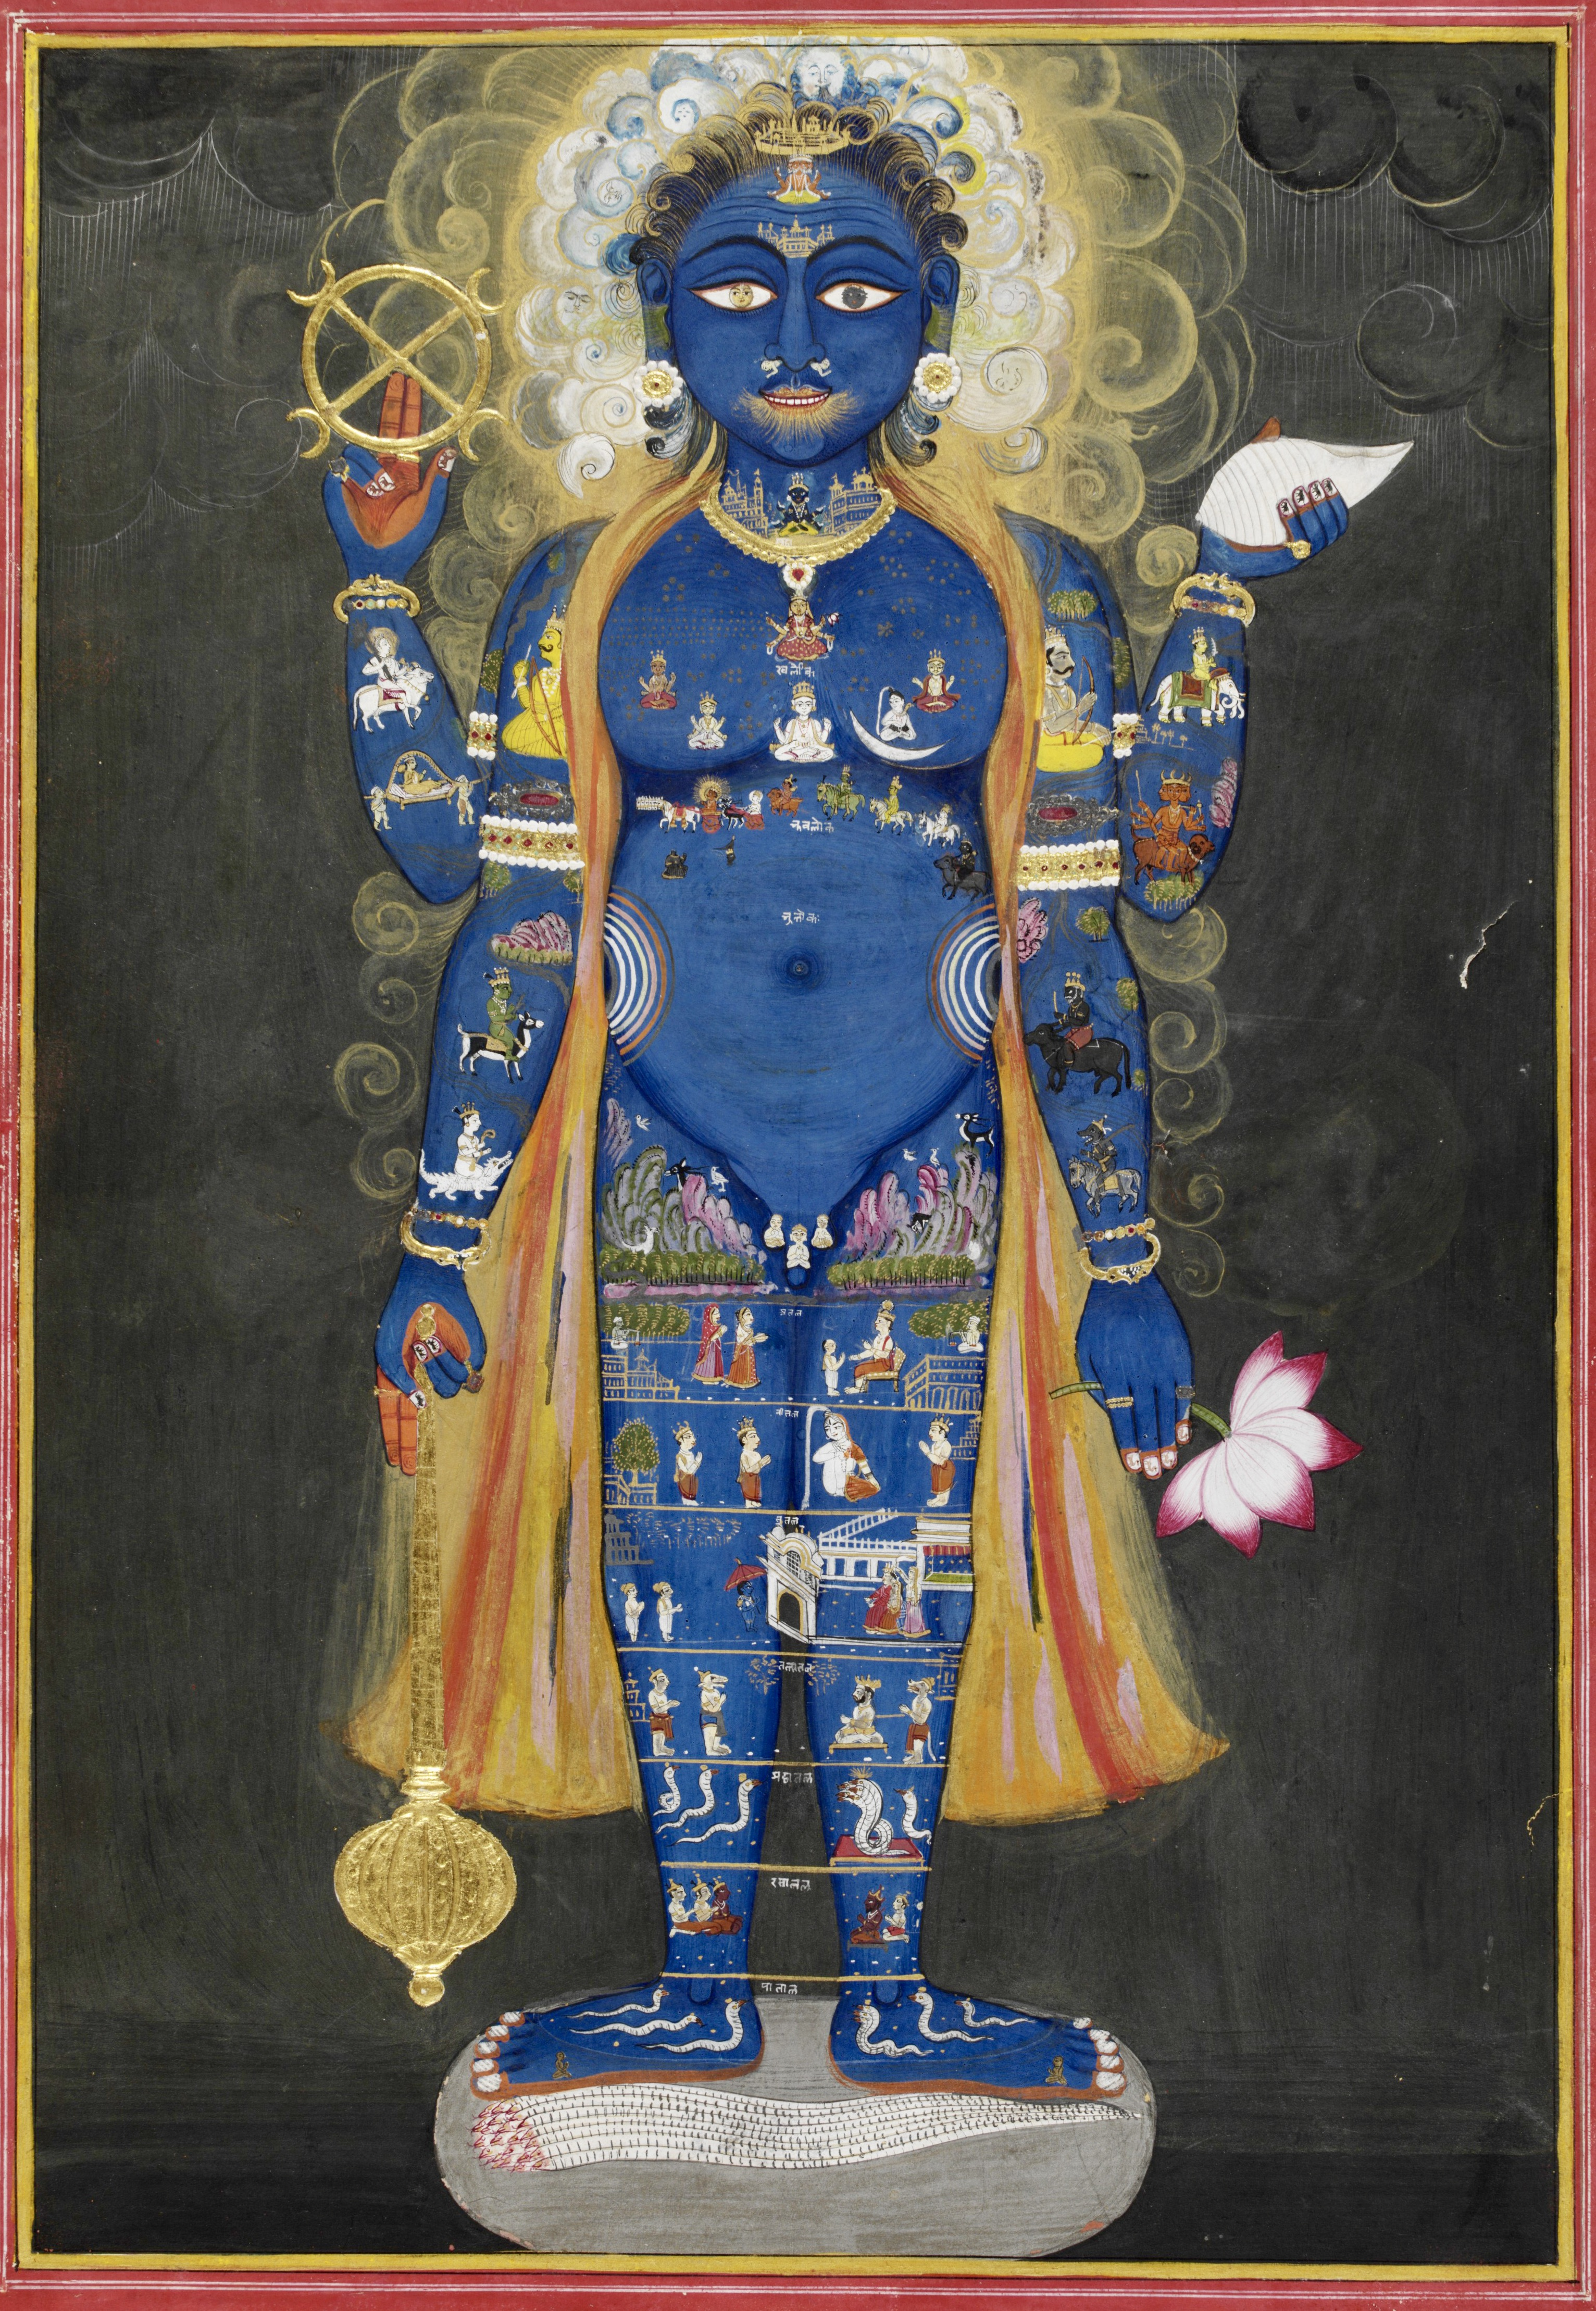
\includegraphics[width=1\textwidth]{pics/Vishnu_Vishvarupa_cropped.jpg}
	\caption{Viṣṇu Viśvarūpa, India, Rajasthan, Jaipur, ca. 1800–1820, Opaque watercolor and gold on paper, 38.5 × 28 cm, Victoria and Albert Museum, London, Given by Mrs. Gerald Clark.}
	\label{fig1}
      \end{figure}
\clearpage
  \begin{figure}[ht]
	\centering
  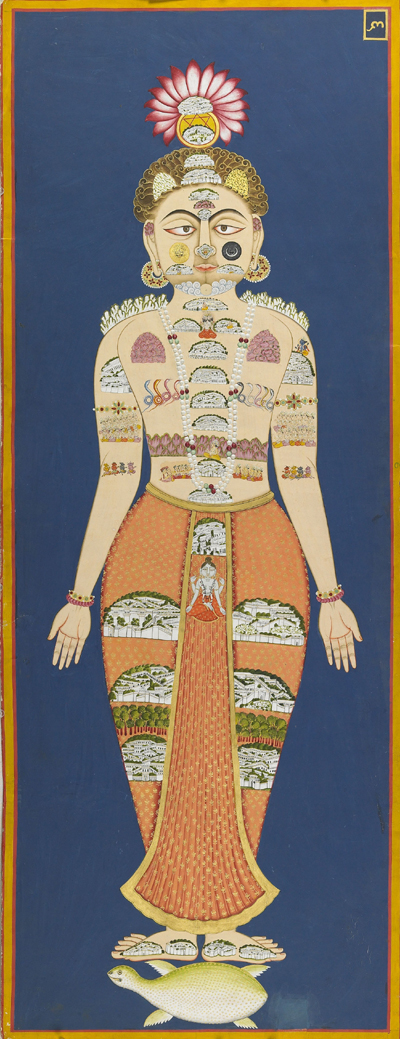
\includegraphics[width=0.5\textwidth]{pics/The_Equivalence_of_Self_and_Universe_(detail),_folio_6_from_the_Siddha_Siddhanta_Paddhati,_(Bulaki),_1824_(Samvat_1881);_122_x_46_cm._Mehrangarh_Museum_Trust..jpg}
	\caption{The Equivalence of Self and Universe (detail), folio 6 from the \textit{Siddhasiddhāntapaddhati} (Bulaki), India, Rajasthan, Jodhpur, 1824 (Samvat 1881), 122 x 46 cm, RJS 2378, Mehragarh Museum Trust.}
	\label{fig2}
      \end{figure}
      % \end{landscape}
\cleardoublepage
\chapter{Bibliography}
 \label{sec:bibli}
\clearpage
\newpage 
\thispagestyle{empty}
\quad  \addtocounter{page}{-1}

\printbibliography[heading=subbibintoc, title=Consulted Manuscripts, keyword=codex]

\printbibliography[heading=subbibintoc, title=Printed Editions, keyword=printsource]

\printbibliography[heading=subbibintoc, title=Secondary Literature, keyword=seclit]

\printbibliography[heading=subbibintoc, title=Online Sources, keyword=onlinesource]

\end{document}


